\documentclass[twoside]{book}

% Packages required by doxygen
\usepackage{fixltx2e}
\usepackage{calc}
\usepackage{doxygen}
\usepackage[export]{adjustbox} % also loads graphicx
\usepackage{graphicx}
\usepackage[utf8]{inputenc}
\usepackage{makeidx}
\usepackage{multicol}
\usepackage{multirow}
\PassOptionsToPackage{warn}{textcomp}
\usepackage{textcomp}
\usepackage[nointegrals]{wasysym}
\usepackage[table]{xcolor}

% Font selection
\usepackage[T1]{fontenc}
\usepackage[scaled=.90]{helvet}
\usepackage{courier}
\usepackage{amssymb}
\usepackage{sectsty}
\renewcommand{\familydefault}{\sfdefault}
\allsectionsfont{%
  \fontseries{bc}\selectfont%
  \color{darkgray}%
}
\renewcommand{\DoxyLabelFont}{%
  \fontseries{bc}\selectfont%
  \color{darkgray}%
}
\newcommand{\+}{\discretionary{\mbox{\scriptsize$\hookleftarrow$}}{}{}}

% Page & text layout
\usepackage{geometry}
\geometry{%
  a4paper,%
  top=2.5cm,%
  bottom=2.5cm,%
  left=2.5cm,%
  right=2.5cm%
}
\tolerance=750
\hfuzz=15pt
\hbadness=750
\setlength{\emergencystretch}{15pt}
\setlength{\parindent}{0cm}
\setlength{\parskip}{3ex plus 2ex minus 2ex}
\makeatletter
\renewcommand{\paragraph}{%
  \@startsection{paragraph}{4}{0ex}{-1.0ex}{1.0ex}{%
    \normalfont\normalsize\bfseries\SS@parafont%
  }%
}
\renewcommand{\subparagraph}{%
  \@startsection{subparagraph}{5}{0ex}{-1.0ex}{1.0ex}{%
    \normalfont\normalsize\bfseries\SS@subparafont%
  }%
}
\makeatother

% Headers & footers
\usepackage{fancyhdr}
\pagestyle{fancyplain}
\fancyhead[LE]{\fancyplain{}{\bfseries\thepage}}
\fancyhead[CE]{\fancyplain{}{}}
\fancyhead[RE]{\fancyplain{}{\bfseries\leftmark}}
\fancyhead[LO]{\fancyplain{}{\bfseries\rightmark}}
\fancyhead[CO]{\fancyplain{}{}}
\fancyhead[RO]{\fancyplain{}{\bfseries\thepage}}
\fancyfoot[LE]{\fancyplain{}{}}
\fancyfoot[CE]{\fancyplain{}{}}
\fancyfoot[RE]{\fancyplain{}{\bfseries\scriptsize Generated by Doxygen }}
\fancyfoot[LO]{\fancyplain{}{\bfseries\scriptsize Generated by Doxygen }}
\fancyfoot[CO]{\fancyplain{}{}}
\fancyfoot[RO]{\fancyplain{}{}}
\renewcommand{\footrulewidth}{0.4pt}
\renewcommand{\chaptermark}[1]{%
  \markboth{#1}{}%
}
\renewcommand{\sectionmark}[1]{%
  \markright{\thesection\ #1}%
}

% Indices & bibliography
\usepackage{natbib}
\usepackage[titles]{tocloft}
\setcounter{tocdepth}{3}
\setcounter{secnumdepth}{5}
\makeindex

% Hyperlinks (required, but should be loaded last)
\usepackage{ifpdf}
\ifpdf
  \usepackage[pdftex,pagebackref=true]{hyperref}
\else
  \usepackage[ps2pdf,pagebackref=true]{hyperref}
\fi
\hypersetup{%
  colorlinks=true,%
  linkcolor=blue,%
  citecolor=blue,%
  unicode%
}

% Custom commands
\newcommand{\clearemptydoublepage}{%
  \newpage{\pagestyle{empty}\cleardoublepage}%
}

\usepackage{caption}
\captionsetup{labelsep=space,justification=centering,font={bf},singlelinecheck=off,skip=4pt,position=top}

%===== C O N T E N T S =====

\begin{document}

% Titlepage & ToC
\hypersetup{pageanchor=false,
             bookmarksnumbered=true,
             pdfencoding=unicode
            }
\pagenumbering{alph}
\begin{titlepage}
\vspace*{7cm}
\begin{center}%
{\Large E\+C\+S\+E211 -\/ Fall 2018 -\/ Final Project \\[1ex]\large 1.\+0 }\\
\vspace*{1cm}
{\large Generated by Doxygen 1.8.13}\\
\end{center}
\end{titlepage}
\clearemptydoublepage
\pagenumbering{roman}
\tableofcontents
\clearemptydoublepage
\pagenumbering{arabic}
\hypersetup{pageanchor=true}

%--- Begin generated contents ---
\chapter{E\+C\+S\+E211-\/\+F2018 Final Project V1.0}
\label{index}\hypertarget{index}{}\section*{Overview\+:}

Documentation for group 5\textquotesingle{}s final project for E\+C\+S\+E211 Fall 2018

\section*{Documentation\+:}

\href{https://ecse211-group5.herokuapp.com/doc/}{\tt Online Javadoc Documentation}

\href{https://ecse211-group5.herokuapp.com/doc/doxygen/html/}{\tt Online Doxygen Documentation}

\section*{List of Open-\/\+Source Projects Used\+:}


\begin{DoxyItemize}
\item Eclipse
\item Le\+Jos
\item Java
\item Doxygen 
\end{DoxyItemize}
\chapter{Namespace Index}
\section{Packages}
Here are the packages with brief descriptions (if available)\+:\begin{DoxyCompactList}
\item\contentsline{section}{\hyperlink{namespaceca}{ca} }{\pageref{namespaceca}}{}
\item\contentsline{section}{\hyperlink{namespaceca_1_1mcgill}{ca.\+mcgill} }{\pageref{namespaceca_1_1mcgill}}{}
\item\contentsline{section}{\hyperlink{namespaceca_1_1mcgill_1_1ecse211}{ca.\+mcgill.\+ecse211} }{\pageref{namespaceca_1_1mcgill_1_1ecse211}}{}
\item\contentsline{section}{\hyperlink{namespaceca_1_1mcgill_1_1ecse211_1_1localization}{ca.\+mcgill.\+ecse211.\+localization} }{\pageref{namespaceca_1_1mcgill_1_1ecse211_1_1localization}}{}
\item\contentsline{section}{\hyperlink{namespaceca_1_1mcgill_1_1ecse211_1_1odometer}{ca.\+mcgill.\+ecse211.\+odometer} }{\pageref{namespaceca_1_1mcgill_1_1ecse211_1_1odometer}}{}
\item\contentsline{section}{\hyperlink{namespaceca_1_1mcgill_1_1ecse211_1_1project}{ca.\+mcgill.\+ecse211.\+project} }{\pageref{namespaceca_1_1mcgill_1_1ecse211_1_1project}}{}
\item\contentsline{section}{\hyperlink{namespaceca_1_1mcgill_1_1ecse211_1_1tests}{ca.\+mcgill.\+ecse211.\+tests} }{\pageref{namespaceca_1_1mcgill_1_1ecse211_1_1tests}}{}
\item\contentsline{section}{\hyperlink{namespaceca_1_1mcgill_1_1ecse211_1_1threads}{ca.\+mcgill.\+ecse211.\+threads} }{\pageref{namespaceca_1_1mcgill_1_1ecse211_1_1threads}}{}
\end{DoxyCompactList}

\chapter{Hierarchical Index}
\section{Class Hierarchy}
This inheritance list is sorted roughly, but not completely, alphabetically\+:\begin{DoxyCompactList}
\item \contentsline{section}{ca.\+mcgill.\+ecse211.\+project.\+Game\+Parameters.\+Area\+Type}{\pageref{enumca_1_1mcgill_1_1ecse211_1_1project_1_1_game_parameters_1_1_area_type}}{}
\item \contentsline{section}{ca.\+mcgill.\+ecse211.\+project.\+Color\+Calibrator}{\pageref{classca_1_1mcgill_1_1ecse211_1_1project_1_1_color_calibrator}}{}
\item \contentsline{section}{ca.\+mcgill.\+ecse211.\+tests.\+Component\+Test}{\pageref{enumca_1_1mcgill_1_1ecse211_1_1tests_1_1_component_test}}{}
\item Exception\begin{DoxyCompactList}
\item \contentsline{section}{ca.\+mcgill.\+ecse211.\+odometer.\+Odometer\+Exceptions}{\pageref{classca_1_1mcgill_1_1ecse211_1_1odometer_1_1_odometer_exceptions}}{}
\end{DoxyCompactList}
\item \contentsline{section}{ca.\+mcgill.\+ecse211.\+project.\+Game}{\pageref{enumca_1_1mcgill_1_1ecse211_1_1project_1_1_game}}{}
\item \contentsline{section}{ca.\+mcgill.\+ecse211.\+project.\+Game\+Parameters}{\pageref{classca_1_1mcgill_1_1ecse211_1_1project_1_1_game_parameters}}{}
\item \contentsline{section}{ca.\+mcgill.\+ecse211.\+localization.\+Light\+Localizer}{\pageref{classca_1_1mcgill_1_1ecse211_1_1localization_1_1_light_localizer}}{}
\item \contentsline{section}{ca.\+mcgill.\+ecse211.\+project.\+Main}{\pageref{classca_1_1mcgill_1_1ecse211_1_1project_1_1_main}}{}
\item \contentsline{section}{ca.\+mcgill.\+ecse211.\+project.\+Navigation}{\pageref{classca_1_1mcgill_1_1ecse211_1_1project_1_1_navigation}}{}
\item \contentsline{section}{ca.\+mcgill.\+ecse211.\+odometer.\+Odometer\+Data}{\pageref{classca_1_1mcgill_1_1ecse211_1_1odometer_1_1_odometer_data}}{}
\begin{DoxyCompactList}
\item \contentsline{section}{ca.\+mcgill.\+ecse211.\+odometer.\+Odometer}{\pageref{classca_1_1mcgill_1_1ecse211_1_1odometer_1_1_odometer}}{}
\end{DoxyCompactList}
\item Runnable\begin{DoxyCompactList}
\item \contentsline{section}{ca.\+mcgill.\+ecse211.\+odometer.\+Odometer}{\pageref{classca_1_1mcgill_1_1ecse211_1_1odometer_1_1_odometer}}{}
\item \contentsline{section}{ca.\+mcgill.\+ecse211.\+odometer.\+Odometry\+Correction}{\pageref{classca_1_1mcgill_1_1ecse211_1_1odometer_1_1_odometry_correction}}{}
\item \contentsline{section}{ca.\+mcgill.\+ecse211.\+project.\+Display}{\pageref{classca_1_1mcgill_1_1ecse211_1_1project_1_1_display}}{}
\item \contentsline{section}{ca.\+mcgill.\+ecse211.\+threads.\+Gyro\+Poller}{\pageref{classca_1_1mcgill_1_1ecse211_1_1threads_1_1_gyro_poller}}{}
\item \contentsline{section}{ca.\+mcgill.\+ecse211.\+threads.\+Thread\+Control}{\pageref{classca_1_1mcgill_1_1ecse211_1_1threads_1_1_thread_control}}{}
\begin{DoxyCompactList}
\item \contentsline{section}{ca.\+mcgill.\+ecse211.\+threads.\+Light\+Poller}{\pageref{classca_1_1mcgill_1_1ecse211_1_1threads_1_1_light_poller}}{}
\begin{DoxyCompactList}
\item \contentsline{section}{ca.\+mcgill.\+ecse211.\+threads.\+R\+G\+B\+Poller}{\pageref{classca_1_1mcgill_1_1ecse211_1_1threads_1_1_r_g_b_poller}}{}
\end{DoxyCompactList}
\item \contentsline{section}{ca.\+mcgill.\+ecse211.\+threads.\+Ring\+Searcher}{\pageref{classca_1_1mcgill_1_1ecse211_1_1threads_1_1_ring_searcher}}{}
\item \contentsline{section}{ca.\+mcgill.\+ecse211.\+threads.\+Ultrasonic\+Poller}{\pageref{classca_1_1mcgill_1_1ecse211_1_1threads_1_1_ultrasonic_poller}}{}
\end{DoxyCompactList}
\end{DoxyCompactList}
\item \contentsline{section}{ca.\+mcgill.\+ecse211.\+threads.\+Sensor\+Data}{\pageref{classca_1_1mcgill_1_1ecse211_1_1threads_1_1_sensor_data}}{}
\item \contentsline{section}{ca.\+mcgill.\+ecse211.\+project.\+Game.\+Status}{\pageref{enumca_1_1mcgill_1_1ecse211_1_1project_1_1_game_1_1_status}}{}
\item \contentsline{section}{ca.\+mcgill.\+ecse211.\+tests.\+Component\+Test.\+Type}{\pageref{enumca_1_1mcgill_1_1ecse211_1_1tests_1_1_component_test_1_1_type}}{}
\item \contentsline{section}{ca.\+mcgill.\+ecse211.\+localization.\+Ultrasonic\+Localizer}{\pageref{classca_1_1mcgill_1_1ecse211_1_1localization_1_1_ultrasonic_localizer}}{}
\item \contentsline{section}{ca.\+mcgill.\+ecse211.\+project.\+Wi\+Fi}{\pageref{classca_1_1mcgill_1_1ecse211_1_1project_1_1_wi_fi}}{}
\end{DoxyCompactList}

\chapter{Class Index}
\section{Class List}
Here are the classes, structs, unions and interfaces with brief descriptions\+:\begin{DoxyCompactList}
\item\contentsline{section}{\hyperlink{classca_1_1mcgill_1_1ecse211_1_1lab5_1_1_color_calibrator}{ca.\+mcgill.\+ecse211.\+lab5.\+Color\+Calibrator} }{\pageref{classca_1_1mcgill_1_1ecse211_1_1lab5_1_1_color_calibrator}}{}
\item\contentsline{section}{\hyperlink{classca_1_1mcgill_1_1ecse211_1_1lab5_1_1_display}{ca.\+mcgill.\+ecse211.\+lab5.\+Display} }{\pageref{classca_1_1mcgill_1_1ecse211_1_1lab5_1_1_display}}{}
\item\contentsline{section}{\hyperlink{classca_1_1mcgill_1_1ecse211_1_1sensors_1_1_gyro_poller}{ca.\+mcgill.\+ecse211.\+sensors.\+Gyro\+Poller} }{\pageref{classca_1_1mcgill_1_1ecse211_1_1sensors_1_1_gyro_poller}}{}
\item\contentsline{section}{\hyperlink{classca_1_1mcgill_1_1ecse211_1_1lab5_1_1_lab5}{ca.\+mcgill.\+ecse211.\+lab5.\+Lab5} }{\pageref{classca_1_1mcgill_1_1ecse211_1_1lab5_1_1_lab5}}{}
\item\contentsline{section}{\hyperlink{classca_1_1mcgill_1_1ecse211_1_1lab5_1_1_light_localizer}{ca.\+mcgill.\+ecse211.\+lab5.\+Light\+Localizer} }{\pageref{classca_1_1mcgill_1_1ecse211_1_1lab5_1_1_light_localizer}}{}
\item\contentsline{section}{\hyperlink{classca_1_1mcgill_1_1ecse211_1_1sensors_1_1_light_poller}{ca.\+mcgill.\+ecse211.\+sensors.\+Light\+Poller} }{\pageref{classca_1_1mcgill_1_1ecse211_1_1sensors_1_1_light_poller}}{}
\item\contentsline{section}{\hyperlink{classca_1_1mcgill_1_1ecse211_1_1lab5_1_1_navigation}{ca.\+mcgill.\+ecse211.\+lab5.\+Navigation} }{\pageref{classca_1_1mcgill_1_1ecse211_1_1lab5_1_1_navigation}}{}
\item\contentsline{section}{\hyperlink{classca_1_1mcgill_1_1ecse211_1_1odometer_1_1_odometer}{ca.\+mcgill.\+ecse211.\+odometer.\+Odometer} }{\pageref{classca_1_1mcgill_1_1ecse211_1_1odometer_1_1_odometer}}{}
\item\contentsline{section}{\hyperlink{classca_1_1mcgill_1_1ecse211_1_1odometer_1_1_odometer_data}{ca.\+mcgill.\+ecse211.\+odometer.\+Odometer\+Data} }{\pageref{classca_1_1mcgill_1_1ecse211_1_1odometer_1_1_odometer_data}}{}
\item\contentsline{section}{\hyperlink{classca_1_1mcgill_1_1ecse211_1_1odometer_1_1_odometer_exceptions}{ca.\+mcgill.\+ecse211.\+odometer.\+Odometer\+Exceptions} }{\pageref{classca_1_1mcgill_1_1ecse211_1_1odometer_1_1_odometer_exceptions}}{}
\item\contentsline{section}{\hyperlink{classca_1_1mcgill_1_1ecse211_1_1odometer_1_1_odometry_correction}{ca.\+mcgill.\+ecse211.\+odometer.\+Odometry\+Correction} }{\pageref{classca_1_1mcgill_1_1ecse211_1_1odometer_1_1_odometry_correction}}{}
\item\contentsline{section}{\hyperlink{classca_1_1mcgill_1_1ecse211_1_1sensors_1_1_r_g_b_poller}{ca.\+mcgill.\+ecse211.\+sensors.\+R\+G\+B\+Poller} }{\pageref{classca_1_1mcgill_1_1ecse211_1_1sensors_1_1_r_g_b_poller}}{}
\item\contentsline{section}{\hyperlink{classca_1_1mcgill_1_1ecse211_1_1lab5_1_1_ring_searcher}{ca.\+mcgill.\+ecse211.\+lab5.\+Ring\+Searcher} }{\pageref{classca_1_1mcgill_1_1ecse211_1_1lab5_1_1_ring_searcher}}{}
\item\contentsline{section}{\hyperlink{classca_1_1mcgill_1_1ecse211_1_1sensors_1_1_sensor_data}{ca.\+mcgill.\+ecse211.\+sensors.\+Sensor\+Data} }{\pageref{classca_1_1mcgill_1_1ecse211_1_1sensors_1_1_sensor_data}}{}
\item\contentsline{section}{\hyperlink{classca_1_1mcgill_1_1ecse211_1_1lab5_1_1_ultrasonic_localizer}{ca.\+mcgill.\+ecse211.\+lab5.\+Ultrasonic\+Localizer} }{\pageref{classca_1_1mcgill_1_1ecse211_1_1lab5_1_1_ultrasonic_localizer}}{}
\item\contentsline{section}{\hyperlink{classca_1_1mcgill_1_1ecse211_1_1sensors_1_1_ultrasonic_poller}{ca.\+mcgill.\+ecse211.\+sensors.\+Ultrasonic\+Poller} }{\pageref{classca_1_1mcgill_1_1ecse211_1_1sensors_1_1_ultrasonic_poller}}{}
\end{DoxyCompactList}

\chapter{File Index}
\section{File List}
Here is a list of all files with brief descriptions\+:\begin{DoxyCompactList}
\item\contentsline{section}{/home/ccc/\+Final\+Project/src/ca/mcgill/ecse211/localization/\hyperlink{_light_localizer_8java}{Light\+Localizer.\+java} }{\pageref{_light_localizer_8java}}{}
\item\contentsline{section}{/home/ccc/\+Final\+Project/src/ca/mcgill/ecse211/localization/\hyperlink{_ultrasonic_localizer_8java}{Ultrasonic\+Localizer.\+java} }{\pageref{_ultrasonic_localizer_8java}}{}
\item\contentsline{section}{/home/ccc/\+Final\+Project/src/ca/mcgill/ecse211/odometer/\hyperlink{_odometer_8java}{Odometer.\+java} }{\pageref{_odometer_8java}}{}
\item\contentsline{section}{/home/ccc/\+Final\+Project/src/ca/mcgill/ecse211/odometer/\hyperlink{_odometer_data_8java}{Odometer\+Data.\+java} }{\pageref{_odometer_data_8java}}{}
\item\contentsline{section}{/home/ccc/\+Final\+Project/src/ca/mcgill/ecse211/odometer/\hyperlink{_odometer_exceptions_8java}{Odometer\+Exceptions.\+java} }{\pageref{_odometer_exceptions_8java}}{}
\item\contentsline{section}{/home/ccc/\+Final\+Project/src/ca/mcgill/ecse211/odometer/\hyperlink{_odometry_correction_8java}{Odometry\+Correction.\+java} }{\pageref{_odometry_correction_8java}}{}
\item\contentsline{section}{/home/ccc/\+Final\+Project/src/ca/mcgill/ecse211/project/\hyperlink{_color_calibrator_8java}{Color\+Calibrator.\+java} }{\pageref{_color_calibrator_8java}}{}
\item\contentsline{section}{/home/ccc/\+Final\+Project/src/ca/mcgill/ecse211/project/\hyperlink{_display_8java}{Display.\+java} }{\pageref{_display_8java}}{}
\item\contentsline{section}{/home/ccc/\+Final\+Project/src/ca/mcgill/ecse211/project/\hyperlink{_game_8java}{Game.\+java} }{\pageref{_game_8java}}{}
\item\contentsline{section}{/home/ccc/\+Final\+Project/src/ca/mcgill/ecse211/project/\hyperlink{_game_parameters_8java}{Game\+Parameters.\+java} }{\pageref{_game_parameters_8java}}{}
\item\contentsline{section}{/home/ccc/\+Final\+Project/src/ca/mcgill/ecse211/project/\hyperlink{_game_util_8java}{Game\+Util.\+java} }{\pageref{_game_util_8java}}{}
\item\contentsline{section}{/home/ccc/\+Final\+Project/src/ca/mcgill/ecse211/project/\hyperlink{_main_8java}{Main.\+java} }{\pageref{_main_8java}}{}
\item\contentsline{section}{/home/ccc/\+Final\+Project/src/ca/mcgill/ecse211/project/\hyperlink{_navigation_8java}{Navigation.\+java} }{\pageref{_navigation_8java}}{}
\item\contentsline{section}{/home/ccc/\+Final\+Project/src/ca/mcgill/ecse211/project/\hyperlink{_wi_fi_8java}{Wi\+Fi.\+java} }{\pageref{_wi_fi_8java}}{}
\item\contentsline{section}{/home/ccc/\+Final\+Project/src/ca/mcgill/ecse211/tests/\hyperlink{_component_test_8java}{Component\+Test.\+java} }{\pageref{_component_test_8java}}{}
\item\contentsline{section}{/home/ccc/\+Final\+Project/src/ca/mcgill/ecse211/threads/\hyperlink{_light_poller_8java}{Light\+Poller.\+java} }{\pageref{_light_poller_8java}}{}
\item\contentsline{section}{/home/ccc/\+Final\+Project/src/ca/mcgill/ecse211/threads/\hyperlink{_r_g_b_poller_8java}{R\+G\+B\+Poller.\+java} }{\pageref{_r_g_b_poller_8java}}{}
\item\contentsline{section}{/home/ccc/\+Final\+Project/src/ca/mcgill/ecse211/threads/\hyperlink{_ring_searcher_8java}{Ring\+Searcher.\+java} }{\pageref{_ring_searcher_8java}}{}
\item\contentsline{section}{/home/ccc/\+Final\+Project/src/ca/mcgill/ecse211/threads/\hyperlink{_sensor_data_8java}{Sensor\+Data.\+java} }{\pageref{_sensor_data_8java}}{}
\item\contentsline{section}{/home/ccc/\+Final\+Project/src/ca/mcgill/ecse211/threads/\hyperlink{_thread_control_8java}{Thread\+Control.\+java} }{\pageref{_thread_control_8java}}{}
\item\contentsline{section}{/home/ccc/\+Final\+Project/src/ca/mcgill/ecse211/threads/\hyperlink{_ultrasonic_poller_8java}{Ultrasonic\+Poller.\+java} }{\pageref{_ultrasonic_poller_8java}}{}
\end{DoxyCompactList}

\chapter{Namespace Documentation}
\hypertarget{namespaceca}{}\section{Package ca}
\label{namespaceca}\index{ca@{ca}}
\subsection*{Packages}
\begin{DoxyCompactItemize}
\item 
package \hyperlink{namespaceca_1_1mcgill}{mcgill}
\end{DoxyCompactItemize}

\hypertarget{namespaceca_1_1mcgill}{}\section{Package ca.\+mcgill}
\label{namespaceca_1_1mcgill}\index{ca.\+mcgill@{ca.\+mcgill}}
\subsection*{Packages}
\begin{DoxyCompactItemize}
\item 
package \hyperlink{namespaceca_1_1mcgill_1_1ecse211}{ecse211}
\end{DoxyCompactItemize}

\hypertarget{namespaceca_1_1mcgill_1_1ecse211}{}\section{Package ca.\+mcgill.\+ecse211}
\label{namespaceca_1_1mcgill_1_1ecse211}\index{ca.\+mcgill.\+ecse211@{ca.\+mcgill.\+ecse211}}
\subsection*{Packages}
\begin{DoxyCompactItemize}
\item 
package \hyperlink{namespaceca_1_1mcgill_1_1ecse211_1_1localization}{localization}
\item 
package \hyperlink{namespaceca_1_1mcgill_1_1ecse211_1_1odometer}{odometer}
\item 
package \hyperlink{namespaceca_1_1mcgill_1_1ecse211_1_1project}{project}
\item 
package \hyperlink{namespaceca_1_1mcgill_1_1ecse211_1_1tests}{tests}
\item 
package \hyperlink{namespaceca_1_1mcgill_1_1ecse211_1_1threads}{threads}
\end{DoxyCompactItemize}

\hypertarget{namespaceca_1_1mcgill_1_1ecse211_1_1localization}{}\section{Package ca.\+mcgill.\+ecse211.\+localization}
\label{namespaceca_1_1mcgill_1_1ecse211_1_1localization}\index{ca.\+mcgill.\+ecse211.\+localization@{ca.\+mcgill.\+ecse211.\+localization}}
\subsection*{Classes}
\begin{DoxyCompactItemize}
\item 
class \hyperlink{classca_1_1mcgill_1_1ecse211_1_1localization_1_1_light_localizer}{Light\+Localizer}
\item 
class \hyperlink{classca_1_1mcgill_1_1ecse211_1_1localization_1_1_ultrasonic_localizer}{Ultrasonic\+Localizer}
\end{DoxyCompactItemize}

\hypertarget{namespaceca_1_1mcgill_1_1ecse211_1_1odometer}{}\section{Package ca.\+mcgill.\+ecse211.\+odometer}
\label{namespaceca_1_1mcgill_1_1ecse211_1_1odometer}\index{ca.\+mcgill.\+ecse211.\+odometer@{ca.\+mcgill.\+ecse211.\+odometer}}
\subsection*{Classes}
\begin{DoxyCompactItemize}
\item 
class \hyperlink{classca_1_1mcgill_1_1ecse211_1_1odometer_1_1_odometer}{Odometer}
\item 
class \hyperlink{classca_1_1mcgill_1_1ecse211_1_1odometer_1_1_odometer_data}{Odometer\+Data}
\item 
class \hyperlink{classca_1_1mcgill_1_1ecse211_1_1odometer_1_1_odometer_exceptions}{Odometer\+Exceptions}
\item 
class \hyperlink{classca_1_1mcgill_1_1ecse211_1_1odometer_1_1_odometry_correction}{Odometry\+Correction}
\end{DoxyCompactItemize}


\subsection{Detailed Description}
This class is meant as a skeleton for the odometer class to be used.

\begin{DoxyAuthor}{Author}
Rodrigo Silva 

Dirk Dubois 

Derek Yu 

Karim El-\/\+Baba 

Michael Smith 
\end{DoxyAuthor}

\hypertarget{namespaceca_1_1mcgill_1_1ecse211_1_1project}{}\section{Package ca.\+mcgill.\+ecse211.\+project}
\label{namespaceca_1_1mcgill_1_1ecse211_1_1project}\index{ca.\+mcgill.\+ecse211.\+project@{ca.\+mcgill.\+ecse211.\+project}}
\subsection*{Classes}
\begin{DoxyCompactItemize}
\item 
class \hyperlink{classca_1_1mcgill_1_1ecse211_1_1project_1_1_color_calibrator}{Color\+Calibrator}
\item 
class \hyperlink{classca_1_1mcgill_1_1ecse211_1_1project_1_1_display}{Display}
\item 
enum \hyperlink{enumca_1_1mcgill_1_1ecse211_1_1project_1_1_game}{Game}
\item 
class \hyperlink{classca_1_1mcgill_1_1ecse211_1_1project_1_1_game_parameters}{Game\+Parameters}
\item 
class \hyperlink{classca_1_1mcgill_1_1ecse211_1_1project_1_1_main}{Main}
\item 
class \hyperlink{classca_1_1mcgill_1_1ecse211_1_1project_1_1_navigation}{Navigation}
\item 
class \hyperlink{classca_1_1mcgill_1_1ecse211_1_1project_1_1_wi_fi}{Wi\+Fi}
\end{DoxyCompactItemize}

\hypertarget{namespaceca_1_1mcgill_1_1ecse211_1_1tests}{}\section{Package ca.\+mcgill.\+ecse211.\+tests}
\label{namespaceca_1_1mcgill_1_1ecse211_1_1tests}\index{ca.\+mcgill.\+ecse211.\+tests@{ca.\+mcgill.\+ecse211.\+tests}}
\subsection*{Classes}
\begin{DoxyCompactItemize}
\item 
enum \hyperlink{enumca_1_1mcgill_1_1ecse211_1_1tests_1_1_component_test}{Component\+Test}
\end{DoxyCompactItemize}

\hypertarget{namespaceca_1_1mcgill_1_1ecse211_1_1threads}{}\section{Package ca.\+mcgill.\+ecse211.\+threads}
\label{namespaceca_1_1mcgill_1_1ecse211_1_1threads}\index{ca.\+mcgill.\+ecse211.\+threads@{ca.\+mcgill.\+ecse211.\+threads}}
\subsection*{Classes}
\begin{DoxyCompactItemize}
\item 
class \hyperlink{classca_1_1mcgill_1_1ecse211_1_1threads_1_1_gyro_poller}{Gyro\+Poller}
\item 
class \hyperlink{classca_1_1mcgill_1_1ecse211_1_1threads_1_1_light_poller}{Light\+Poller}
\item 
class \hyperlink{classca_1_1mcgill_1_1ecse211_1_1threads_1_1_r_g_b_poller}{R\+G\+B\+Poller}
\item 
class \hyperlink{classca_1_1mcgill_1_1ecse211_1_1threads_1_1_ring_searcher}{Ring\+Searcher}
\item 
class \hyperlink{classca_1_1mcgill_1_1ecse211_1_1threads_1_1_sensor_data}{Sensor\+Data}
\item 
class \hyperlink{classca_1_1mcgill_1_1ecse211_1_1threads_1_1_thread_control}{Thread\+Control}
\item 
class \hyperlink{classca_1_1mcgill_1_1ecse211_1_1threads_1_1_ultrasonic_poller}{Ultrasonic\+Poller}
\end{DoxyCompactItemize}

\chapter{Class Documentation}
\hypertarget{enumca_1_1mcgill_1_1ecse211_1_1project_1_1_game_parameters_1_1_area_type}{}\section{ca.\+mcgill.\+ecse211.\+project.\+Game\+Parameters.\+Area\+Type Enum Reference}
\label{enumca_1_1mcgill_1_1ecse211_1_1project_1_1_game_parameters_1_1_area_type}\index{ca.\+mcgill.\+ecse211.\+project.\+Game\+Parameters.\+Area\+Type@{ca.\+mcgill.\+ecse211.\+project.\+Game\+Parameters.\+Area\+Type}}
\subsection*{Public Attributes}
\begin{DoxyCompactItemize}
\item 
\hyperlink{enumca_1_1mcgill_1_1ecse211_1_1project_1_1_game_parameters_1_1_area_type_a90e9cb33114c7af62aa86684942265e5}{In\+Starting}
\item 
\hyperlink{enumca_1_1mcgill_1_1ecse211_1_1project_1_1_game_parameters_1_1_area_type_a25564076fdd8880377fbd6eaf753456f}{Searching}
\item 
\hyperlink{enumca_1_1mcgill_1_1ecse211_1_1project_1_1_game_parameters_1_1_area_type_ac762256f8b33e7c93c162520a0349769}{Dangerous}
\item 
\hyperlink{enumca_1_1mcgill_1_1ecse211_1_1project_1_1_game_parameters_1_1_area_type_afd78c1184c6b82e22bb08ed39ae4e83b}{Starting\+Boundary}
\item 
\hyperlink{enumca_1_1mcgill_1_1ecse211_1_1project_1_1_game_parameters_1_1_area_type_a5a3aceb665ba97ac242e77955feed640}{Searching\+Boundary}
\end{DoxyCompactItemize}


\subsection{Detailed Description}
This enumeration contains the possible types of areas that our robot is currently located in 

Definition at line 18 of file Game\+Parameters.\+java.



\subsection{Member Data Documentation}
\mbox{\Hypertarget{enumca_1_1mcgill_1_1ecse211_1_1project_1_1_game_parameters_1_1_area_type_ac762256f8b33e7c93c162520a0349769}\label{enumca_1_1mcgill_1_1ecse211_1_1project_1_1_game_parameters_1_1_area_type_ac762256f8b33e7c93c162520a0349769}} 
\index{ca\+::mcgill\+::ecse211\+::project\+::\+Game\+Parameters\+::\+Area\+Type@{ca\+::mcgill\+::ecse211\+::project\+::\+Game\+Parameters\+::\+Area\+Type}!Dangerous@{Dangerous}}
\index{Dangerous@{Dangerous}!ca\+::mcgill\+::ecse211\+::project\+::\+Game\+Parameters\+::\+Area\+Type@{ca\+::mcgill\+::ecse211\+::project\+::\+Game\+Parameters\+::\+Area\+Type}}
\subsubsection{\texorpdfstring{Dangerous}{Dangerous}}
{\footnotesize\ttfamily ca.\+mcgill.\+ecse211.\+project.\+Game\+Parameters.\+Area\+Type.\+Dangerous}



Definition at line 19 of file Game\+Parameters.\+java.

\mbox{\Hypertarget{enumca_1_1mcgill_1_1ecse211_1_1project_1_1_game_parameters_1_1_area_type_a90e9cb33114c7af62aa86684942265e5}\label{enumca_1_1mcgill_1_1ecse211_1_1project_1_1_game_parameters_1_1_area_type_a90e9cb33114c7af62aa86684942265e5}} 
\index{ca\+::mcgill\+::ecse211\+::project\+::\+Game\+Parameters\+::\+Area\+Type@{ca\+::mcgill\+::ecse211\+::project\+::\+Game\+Parameters\+::\+Area\+Type}!In\+Starting@{In\+Starting}}
\index{In\+Starting@{In\+Starting}!ca\+::mcgill\+::ecse211\+::project\+::\+Game\+Parameters\+::\+Area\+Type@{ca\+::mcgill\+::ecse211\+::project\+::\+Game\+Parameters\+::\+Area\+Type}}
\subsubsection{\texorpdfstring{In\+Starting}{InStarting}}
{\footnotesize\ttfamily ca.\+mcgill.\+ecse211.\+project.\+Game\+Parameters.\+Area\+Type.\+In\+Starting}



Definition at line 19 of file Game\+Parameters.\+java.

\mbox{\Hypertarget{enumca_1_1mcgill_1_1ecse211_1_1project_1_1_game_parameters_1_1_area_type_a25564076fdd8880377fbd6eaf753456f}\label{enumca_1_1mcgill_1_1ecse211_1_1project_1_1_game_parameters_1_1_area_type_a25564076fdd8880377fbd6eaf753456f}} 
\index{ca\+::mcgill\+::ecse211\+::project\+::\+Game\+Parameters\+::\+Area\+Type@{ca\+::mcgill\+::ecse211\+::project\+::\+Game\+Parameters\+::\+Area\+Type}!Searching@{Searching}}
\index{Searching@{Searching}!ca\+::mcgill\+::ecse211\+::project\+::\+Game\+Parameters\+::\+Area\+Type@{ca\+::mcgill\+::ecse211\+::project\+::\+Game\+Parameters\+::\+Area\+Type}}
\subsubsection{\texorpdfstring{Searching}{Searching}}
{\footnotesize\ttfamily ca.\+mcgill.\+ecse211.\+project.\+Game\+Parameters.\+Area\+Type.\+Searching}



Definition at line 19 of file Game\+Parameters.\+java.

\mbox{\Hypertarget{enumca_1_1mcgill_1_1ecse211_1_1project_1_1_game_parameters_1_1_area_type_a5a3aceb665ba97ac242e77955feed640}\label{enumca_1_1mcgill_1_1ecse211_1_1project_1_1_game_parameters_1_1_area_type_a5a3aceb665ba97ac242e77955feed640}} 
\index{ca\+::mcgill\+::ecse211\+::project\+::\+Game\+Parameters\+::\+Area\+Type@{ca\+::mcgill\+::ecse211\+::project\+::\+Game\+Parameters\+::\+Area\+Type}!Searching\+Boundary@{Searching\+Boundary}}
\index{Searching\+Boundary@{Searching\+Boundary}!ca\+::mcgill\+::ecse211\+::project\+::\+Game\+Parameters\+::\+Area\+Type@{ca\+::mcgill\+::ecse211\+::project\+::\+Game\+Parameters\+::\+Area\+Type}}
\subsubsection{\texorpdfstring{Searching\+Boundary}{SearchingBoundary}}
{\footnotesize\ttfamily ca.\+mcgill.\+ecse211.\+project.\+Game\+Parameters.\+Area\+Type.\+Searching\+Boundary}



Definition at line 19 of file Game\+Parameters.\+java.

\mbox{\Hypertarget{enumca_1_1mcgill_1_1ecse211_1_1project_1_1_game_parameters_1_1_area_type_afd78c1184c6b82e22bb08ed39ae4e83b}\label{enumca_1_1mcgill_1_1ecse211_1_1project_1_1_game_parameters_1_1_area_type_afd78c1184c6b82e22bb08ed39ae4e83b}} 
\index{ca\+::mcgill\+::ecse211\+::project\+::\+Game\+Parameters\+::\+Area\+Type@{ca\+::mcgill\+::ecse211\+::project\+::\+Game\+Parameters\+::\+Area\+Type}!Starting\+Boundary@{Starting\+Boundary}}
\index{Starting\+Boundary@{Starting\+Boundary}!ca\+::mcgill\+::ecse211\+::project\+::\+Game\+Parameters\+::\+Area\+Type@{ca\+::mcgill\+::ecse211\+::project\+::\+Game\+Parameters\+::\+Area\+Type}}
\subsubsection{\texorpdfstring{Starting\+Boundary}{StartingBoundary}}
{\footnotesize\ttfamily ca.\+mcgill.\+ecse211.\+project.\+Game\+Parameters.\+Area\+Type.\+Starting\+Boundary}



Definition at line 19 of file Game\+Parameters.\+java.



The documentation for this enum was generated from the following file\+:\begin{DoxyCompactItemize}
\item 
/home/ccc/\+Final\+Project/src/ca/mcgill/ecse211/project/\hyperlink{_game_parameters_8java}{Game\+Parameters.\+java}\end{DoxyCompactItemize}

\hypertarget{classca_1_1mcgill_1_1ecse211_1_1project_1_1_color_calibrator}{}\section{ca.\+mcgill.\+ecse211.\+project.\+Color\+Calibrator Class Reference}
\label{classca_1_1mcgill_1_1ecse211_1_1project_1_1_color_calibrator}\index{ca.\+mcgill.\+ecse211.\+project.\+Color\+Calibrator@{ca.\+mcgill.\+ecse211.\+project.\+Color\+Calibrator}}
\subsection*{Classes}
\begin{DoxyCompactItemize}
\item 
enum {\bfseries Color}
\end{DoxyCompactItemize}
\subsection*{Static Public Member Functions}
\begin{DoxyCompactItemize}
\item 
static Color \hyperlink{classca_1_1mcgill_1_1ecse211_1_1project_1_1_color_calibrator_a92e653a6a9f7a31cb7b6f9bc2e732133}{get\+Color} (int r, int g, int b)
\item 
static Color \hyperlink{classca_1_1mcgill_1_1ecse211_1_1project_1_1_color_calibrator_a1acf05f9523b2c0f329d4a7cbf1b9c47}{get\+Color} ()
\item 
static void \hyperlink{classca_1_1mcgill_1_1ecse211_1_1project_1_1_color_calibrator_a40906193773ead0bfd582f188413c97a}{set\+Frequency} (Color c)
\item 
static Color \hyperlink{classca_1_1mcgill_1_1ecse211_1_1project_1_1_color_calibrator_a3d65927aaa2041f933dbdc19c3d2a412}{get\+Most\+Frequenct} ()
\item 
static void \hyperlink{classca_1_1mcgill_1_1ecse211_1_1project_1_1_color_calibrator_ab6148d75e3a105016580e90ed1ea9bc9}{reset\+Frequency} ()
\item 
static Color \hyperlink{classca_1_1mcgill_1_1ecse211_1_1project_1_1_color_calibrator_acb1d9cef0739971dbe00cc16712be0fe}{get\+Get\+Color} (int i)
\end{DoxyCompactItemize}


\subsection{Detailed Description}
This class is used to check the color of a ring under a light sensor

\begin{DoxyAuthor}{Author}
Caspar Cedro 

Percy Chen 

Patrick Erath 

Anssam Ghezala 

Susan Matuszewski 

Kamy Moussavi Kafi 
\end{DoxyAuthor}


Definition at line 13 of file Color\+Calibrator.\+java.



\subsection{Member Function Documentation}
\mbox{\Hypertarget{classca_1_1mcgill_1_1ecse211_1_1project_1_1_color_calibrator_a92e653a6a9f7a31cb7b6f9bc2e732133}\label{classca_1_1mcgill_1_1ecse211_1_1project_1_1_color_calibrator_a92e653a6a9f7a31cb7b6f9bc2e732133}} 
\index{ca\+::mcgill\+::ecse211\+::project\+::\+Color\+Calibrator@{ca\+::mcgill\+::ecse211\+::project\+::\+Color\+Calibrator}!get\+Color@{get\+Color}}
\index{get\+Color@{get\+Color}!ca\+::mcgill\+::ecse211\+::project\+::\+Color\+Calibrator@{ca\+::mcgill\+::ecse211\+::project\+::\+Color\+Calibrator}}
\subsubsection{\texorpdfstring{get\+Color()}{getColor()}\hspace{0.1cm}{\footnotesize\ttfamily [1/2]}}
{\footnotesize\ttfamily static Color ca.\+mcgill.\+ecse211.\+project.\+Color\+Calibrator.\+get\+Color (\begin{DoxyParamCaption}\item[{int}]{r,  }\item[{int}]{g,  }\item[{int}]{b }\end{DoxyParamCaption})\hspace{0.3cm}{\ttfamily [static]}}

This method returns the color of the ring currently under the light sensor Instead of intervals, we use a pattern matching for detecting the color For more\+: reference the software and testing document


\begin{DoxyParams}{Parameters}
{\em r} & The red value to check for a ring \\
\hline
{\em g} & The green value to check for a ring \\
\hline
{\em b} & The blue value to check for a ring \\
\hline
\end{DoxyParams}
\begin{DoxyReturn}{Returns}
A Color enumeration value 
\end{DoxyReturn}


Definition at line 37 of file Color\+Calibrator.\+java.


\begin{DoxyCode}
37                                                     \{
38     \textcolor{keywordflow}{if} (r>3*g && b<3 && r>lowerOrangeRBound ) \{
39       currentColor = Color.Orange;
40     \} \textcolor{keywordflow}{else} \textcolor{keywordflow}{if} (g>r && b<3) \{
41       currentColor = Color.Green;
42       \}\textcolor{keywordflow}{else} \textcolor{keywordflow}{if} ((r>= lowerYellowRBound && g >= lowerYellowGBound) || ((r>= 7 && r <= 9) && (g >=0 && g <= 2
      ))) \{
43       currentColor = Color.Yellow;
44     \} \textcolor{keywordflow}{else} \textcolor{keywordflow}{if} ( (b >= lowerBlueBBound )) \{
45       currentColor = Color.Blue;
46     \} \textcolor{keywordflow}{else} \{
47       currentColor = Color.Other;
48     \}
49 
50     \textcolor{keywordflow}{return} currentColor;
51   \}
\end{DoxyCode}
Here is the caller graph for this function\+:\nopagebreak
\begin{figure}[H]
\begin{center}
\leavevmode
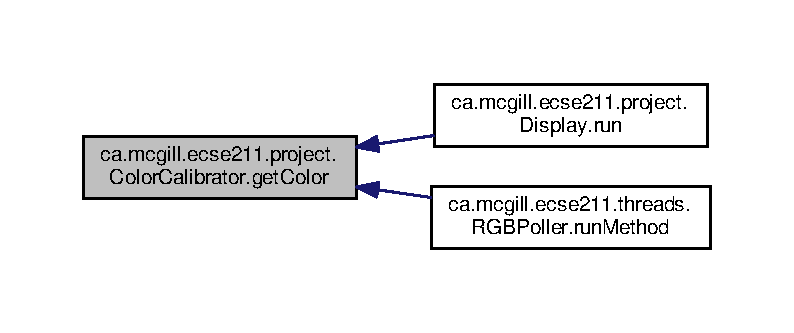
\includegraphics[width=350pt]{classca_1_1mcgill_1_1ecse211_1_1project_1_1_color_calibrator_a92e653a6a9f7a31cb7b6f9bc2e732133_icgraph}
\end{center}
\end{figure}
\mbox{\Hypertarget{classca_1_1mcgill_1_1ecse211_1_1project_1_1_color_calibrator_a1acf05f9523b2c0f329d4a7cbf1b9c47}\label{classca_1_1mcgill_1_1ecse211_1_1project_1_1_color_calibrator_a1acf05f9523b2c0f329d4a7cbf1b9c47}} 
\index{ca\+::mcgill\+::ecse211\+::project\+::\+Color\+Calibrator@{ca\+::mcgill\+::ecse211\+::project\+::\+Color\+Calibrator}!get\+Color@{get\+Color}}
\index{get\+Color@{get\+Color}!ca\+::mcgill\+::ecse211\+::project\+::\+Color\+Calibrator@{ca\+::mcgill\+::ecse211\+::project\+::\+Color\+Calibrator}}
\subsubsection{\texorpdfstring{get\+Color()}{getColor()}\hspace{0.1cm}{\footnotesize\ttfamily [2/2]}}
{\footnotesize\ttfamily static Color ca.\+mcgill.\+ecse211.\+project.\+Color\+Calibrator.\+get\+Color (\begin{DoxyParamCaption}{ }\end{DoxyParamCaption})\hspace{0.3cm}{\ttfamily [static]}}

This method gets the last color of the ring under the light sensor

\begin{DoxyReturn}{Returns}
current color detected by the light\+Sensor 
\end{DoxyReturn}


Definition at line 58 of file Color\+Calibrator.\+java.


\begin{DoxyCode}
58                                  \{
59     \textcolor{keywordflow}{if} (currentColor != null)
60       \textcolor{keywordflow}{return} currentColor;
61     \textcolor{keywordflow}{else}
62       \textcolor{keywordflow}{return} Color.Other;
63   \}
\end{DoxyCode}
\mbox{\Hypertarget{classca_1_1mcgill_1_1ecse211_1_1project_1_1_color_calibrator_acb1d9cef0739971dbe00cc16712be0fe}\label{classca_1_1mcgill_1_1ecse211_1_1project_1_1_color_calibrator_acb1d9cef0739971dbe00cc16712be0fe}} 
\index{ca\+::mcgill\+::ecse211\+::project\+::\+Color\+Calibrator@{ca\+::mcgill\+::ecse211\+::project\+::\+Color\+Calibrator}!get\+Get\+Color@{get\+Get\+Color}}
\index{get\+Get\+Color@{get\+Get\+Color}!ca\+::mcgill\+::ecse211\+::project\+::\+Color\+Calibrator@{ca\+::mcgill\+::ecse211\+::project\+::\+Color\+Calibrator}}
\subsubsection{\texorpdfstring{get\+Get\+Color()}{getGetColor()}}
{\footnotesize\ttfamily static Color ca.\+mcgill.\+ecse211.\+project.\+Color\+Calibrator.\+get\+Get\+Color (\begin{DoxyParamCaption}\item[{int}]{i }\end{DoxyParamCaption})\hspace{0.3cm}{\ttfamily [static]}}

This method match integer to corresponding color 
\begin{DoxyParams}{Parameters}
{\em i} & an integer of \mbox{[}0,4\mbox{]} \\
\hline
\end{DoxyParams}
\begin{DoxyReturn}{Returns}
\+: cooresponding color of the integer 
\end{DoxyReturn}


Definition at line 124 of file Color\+Calibrator.\+java.


\begin{DoxyCode}
124                                          \{
125     Color c = Color.Other;
126     \textcolor{keywordflow}{switch} (i) \{
127       \textcolor{keywordflow}{case} 0:
128         c = Color.Other;
129         \textcolor{keywordflow}{break};
130       \textcolor{keywordflow}{case} 1: 
131         c = Color.Blue;
132         \textcolor{keywordflow}{break};
133       \textcolor{keywordflow}{case} 2:
134         c = Color.Green;
135         \textcolor{keywordflow}{break};
136       \textcolor{keywordflow}{case} 3:
137         c = Color.Yellow;
138         \textcolor{keywordflow}{break};
139       \textcolor{keywordflow}{case} 4:
140         c = Color.Orange;
141         \textcolor{keywordflow}{break};
142     \}
143     \textcolor{keywordflow}{return} c;
144   \}
\end{DoxyCode}
Here is the caller graph for this function\+:
\nopagebreak
\begin{figure}[H]
\begin{center}
\leavevmode
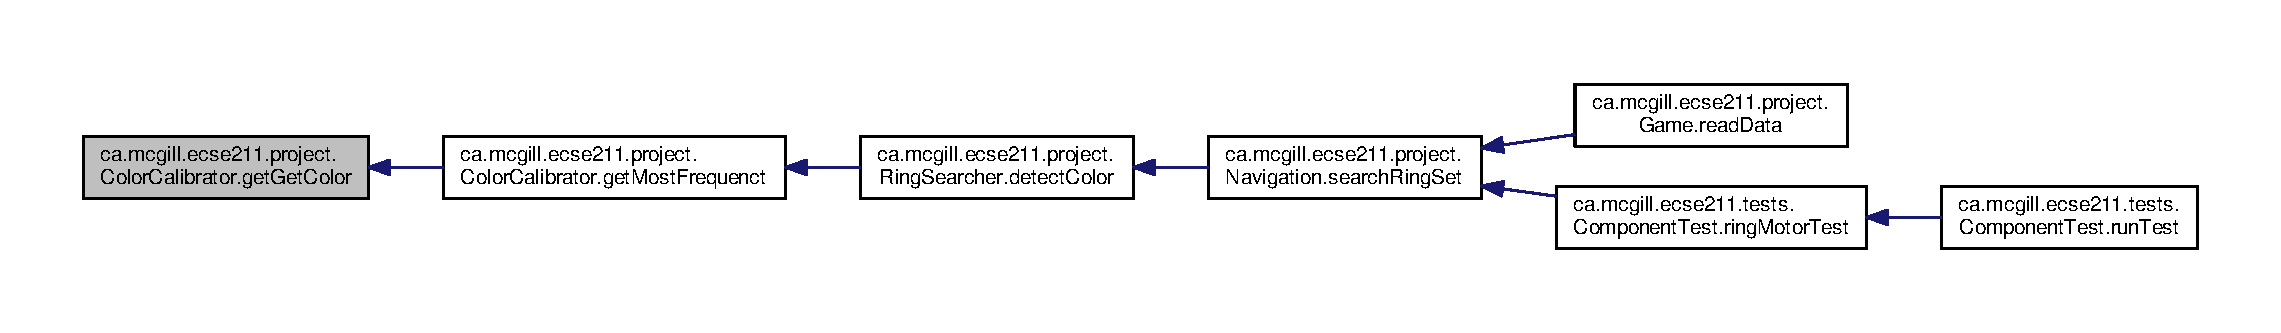
\includegraphics[width=350pt]{classca_1_1mcgill_1_1ecse211_1_1project_1_1_color_calibrator_acb1d9cef0739971dbe00cc16712be0fe_icgraph}
\end{center}
\end{figure}
\mbox{\Hypertarget{classca_1_1mcgill_1_1ecse211_1_1project_1_1_color_calibrator_a3d65927aaa2041f933dbdc19c3d2a412}\label{classca_1_1mcgill_1_1ecse211_1_1project_1_1_color_calibrator_a3d65927aaa2041f933dbdc19c3d2a412}} 
\index{ca\+::mcgill\+::ecse211\+::project\+::\+Color\+Calibrator@{ca\+::mcgill\+::ecse211\+::project\+::\+Color\+Calibrator}!get\+Most\+Frequenct@{get\+Most\+Frequenct}}
\index{get\+Most\+Frequenct@{get\+Most\+Frequenct}!ca\+::mcgill\+::ecse211\+::project\+::\+Color\+Calibrator@{ca\+::mcgill\+::ecse211\+::project\+::\+Color\+Calibrator}}
\subsubsection{\texorpdfstring{get\+Most\+Frequenct()}{getMostFrequenct()}}
{\footnotesize\ttfamily static Color ca.\+mcgill.\+ecse211.\+project.\+Color\+Calibrator.\+get\+Most\+Frequenct (\begin{DoxyParamCaption}{ }\end{DoxyParamCaption})\hspace{0.3cm}{\ttfamily [static]}}

This method returns the most frequent colour detected from multiple samples

\begin{DoxyReturn}{Returns}
most frequent colour detected 
\end{DoxyReturn}


Definition at line 93 of file Color\+Calibrator.\+java.


\begin{DoxyCode}
93                                          \{
94     Color c = Color.Other;
95     \textcolor{keywordtype}{int} frequency = colour\_frequency[0];
96     \textcolor{keywordflow}{for} (\textcolor{keywordtype}{int} i = 0; i < colour\_frequency.length; i++) \{
97       \textcolor{keywordflow}{if} (colour\_frequency[i] >= frequency) \{
98         frequency = colour\_frequency[i];
99         c = \hyperlink{classca_1_1mcgill_1_1ecse211_1_1project_1_1_color_calibrator_acb1d9cef0739971dbe00cc16712be0fe}{getGetColor}(i);
100       \}
101     \}
102     \textcolor{keywordflow}{if}(frequency == 0) \{
103       c = Color.Other;
104     \}
105     \hyperlink{classca_1_1mcgill_1_1ecse211_1_1project_1_1_color_calibrator_ab6148d75e3a105016580e90ed1ea9bc9}{resetFrequency}();
106     \textcolor{keywordflow}{return} c;
107   \}
\end{DoxyCode}
Here is the call graph for this function\+:
\nopagebreak
\begin{figure}[H]
\begin{center}
\leavevmode
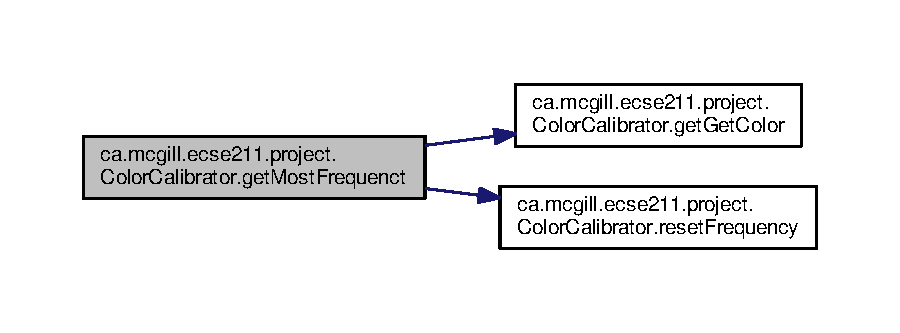
\includegraphics[width=350pt]{classca_1_1mcgill_1_1ecse211_1_1project_1_1_color_calibrator_a3d65927aaa2041f933dbdc19c3d2a412_cgraph}
\end{center}
\end{figure}
Here is the caller graph for this function\+:
\nopagebreak
\begin{figure}[H]
\begin{center}
\leavevmode
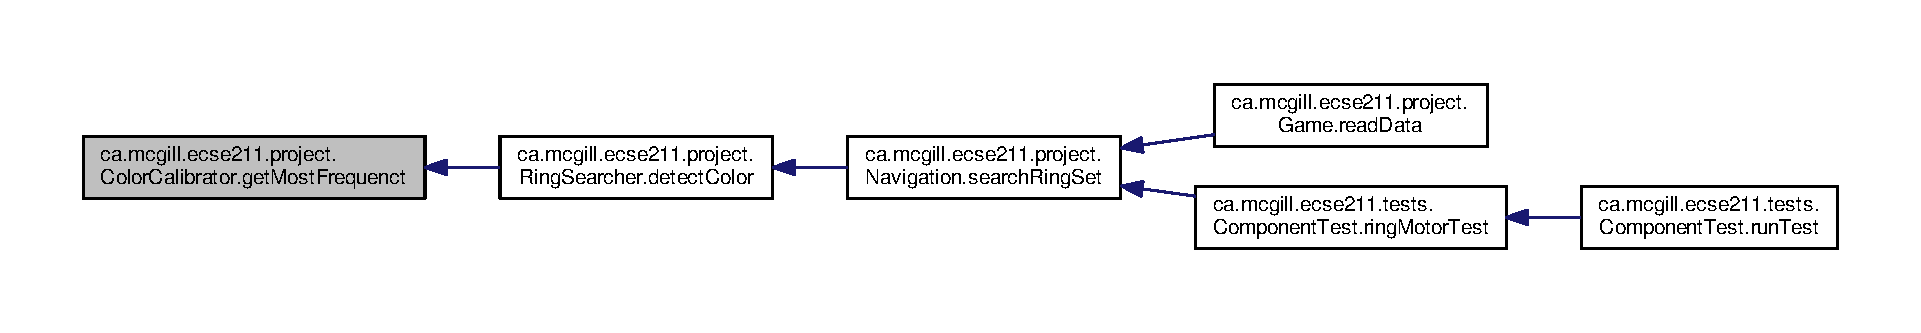
\includegraphics[width=350pt]{classca_1_1mcgill_1_1ecse211_1_1project_1_1_color_calibrator_a3d65927aaa2041f933dbdc19c3d2a412_icgraph}
\end{center}
\end{figure}
\mbox{\Hypertarget{classca_1_1mcgill_1_1ecse211_1_1project_1_1_color_calibrator_ab6148d75e3a105016580e90ed1ea9bc9}\label{classca_1_1mcgill_1_1ecse211_1_1project_1_1_color_calibrator_ab6148d75e3a105016580e90ed1ea9bc9}} 
\index{ca\+::mcgill\+::ecse211\+::project\+::\+Color\+Calibrator@{ca\+::mcgill\+::ecse211\+::project\+::\+Color\+Calibrator}!reset\+Frequency@{reset\+Frequency}}
\index{reset\+Frequency@{reset\+Frequency}!ca\+::mcgill\+::ecse211\+::project\+::\+Color\+Calibrator@{ca\+::mcgill\+::ecse211\+::project\+::\+Color\+Calibrator}}
\subsubsection{\texorpdfstring{reset\+Frequency()}{resetFrequency()}}
{\footnotesize\ttfamily static void ca.\+mcgill.\+ecse211.\+project.\+Color\+Calibrator.\+reset\+Frequency (\begin{DoxyParamCaption}{ }\end{DoxyParamCaption})\hspace{0.3cm}{\ttfamily [static]}}

This method resets the colour\+\_\+frequency array to 0 

Definition at line 113 of file Color\+Calibrator.\+java.


\begin{DoxyCode}
113                                       \{
114     \textcolor{keywordflow}{for} (\textcolor{keywordtype}{int} i = 0; i < colour\_frequency.length; i ++) \{
115       colour\_frequency[i] = 0;
116     \}
117   \}
\end{DoxyCode}
Here is the caller graph for this function\+:
\nopagebreak
\begin{figure}[H]
\begin{center}
\leavevmode
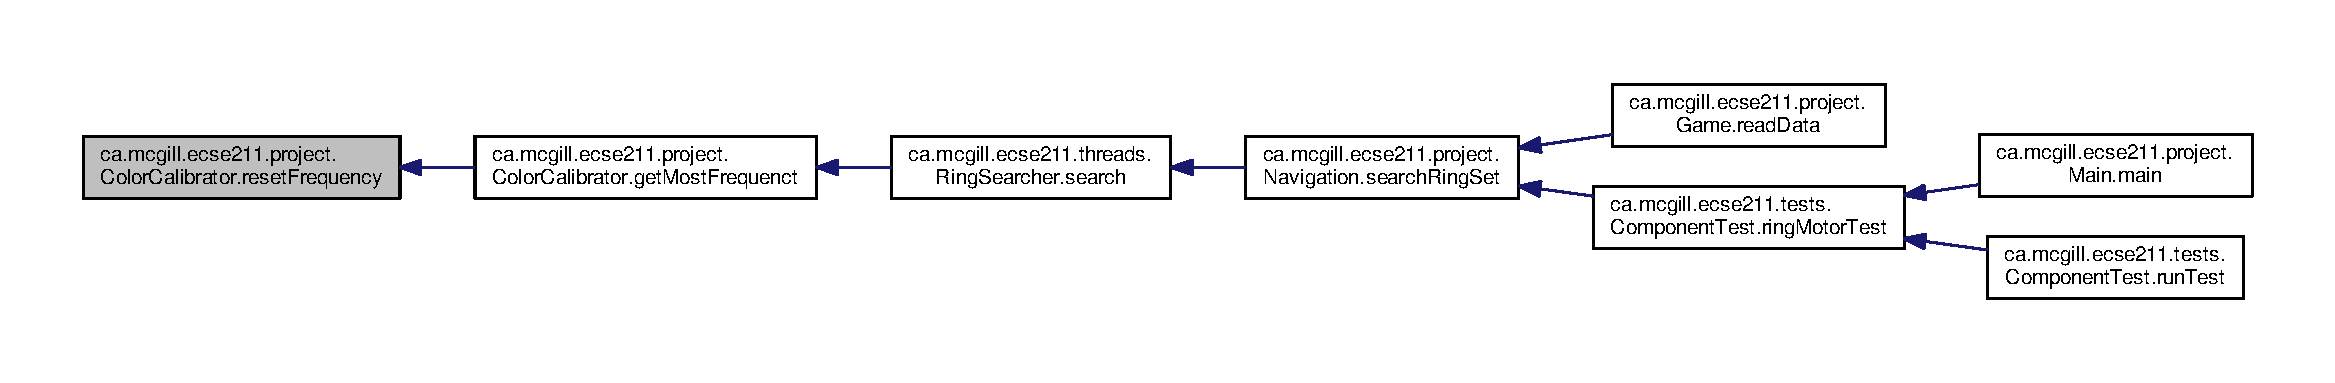
\includegraphics[width=350pt]{classca_1_1mcgill_1_1ecse211_1_1project_1_1_color_calibrator_ab6148d75e3a105016580e90ed1ea9bc9_icgraph}
\end{center}
\end{figure}
\mbox{\Hypertarget{classca_1_1mcgill_1_1ecse211_1_1project_1_1_color_calibrator_a40906193773ead0bfd582f188413c97a}\label{classca_1_1mcgill_1_1ecse211_1_1project_1_1_color_calibrator_a40906193773ead0bfd582f188413c97a}} 
\index{ca\+::mcgill\+::ecse211\+::project\+::\+Color\+Calibrator@{ca\+::mcgill\+::ecse211\+::project\+::\+Color\+Calibrator}!set\+Frequency@{set\+Frequency}}
\index{set\+Frequency@{set\+Frequency}!ca\+::mcgill\+::ecse211\+::project\+::\+Color\+Calibrator@{ca\+::mcgill\+::ecse211\+::project\+::\+Color\+Calibrator}}
\subsubsection{\texorpdfstring{set\+Frequency()}{setFrequency()}}
{\footnotesize\ttfamily static void ca.\+mcgill.\+ecse211.\+project.\+Color\+Calibrator.\+set\+Frequency (\begin{DoxyParamCaption}\item[{Color}]{c }\end{DoxyParamCaption})\hspace{0.3cm}{\ttfamily [static]}}

This method keeps track of how many of each colour were detected by increasing the count in the array 
\begin{DoxyParams}{Parameters}
{\em c} & The Color detected by the light sensor \\
\hline
\end{DoxyParams}


Definition at line 70 of file Color\+Calibrator.\+java.


\begin{DoxyCode}
70                                            \{
71     \textcolor{keywordflow}{switch} (c) \{
72       \textcolor{keywordflow}{case} Blue:
73         colour\_frequency[1] ++;
74         \textcolor{keywordflow}{break};
75       \textcolor{keywordflow}{case} Green:
76         colour\_frequency[2] ++;
77         \textcolor{keywordflow}{break};
78       \textcolor{keywordflow}{case} Yellow:
79         colour\_frequency[3] ++;
80         \textcolor{keywordflow}{break};
81       \textcolor{keywordflow}{case} Orange:
82         colour\_frequency[4] ++;
83       \textcolor{keywordflow}{default}:
84         \textcolor{keywordflow}{break};
85     \}
86   \}
\end{DoxyCode}
Here is the caller graph for this function\+:
\nopagebreak
\begin{figure}[H]
\begin{center}
\leavevmode
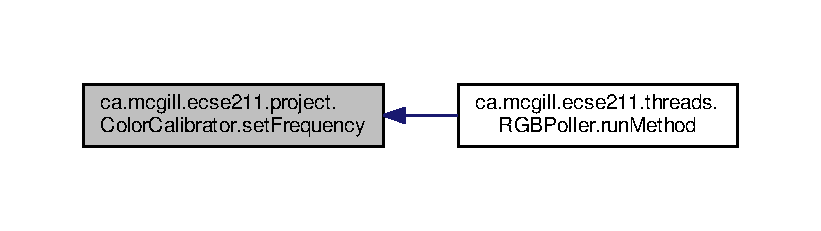
\includegraphics[width=350pt]{classca_1_1mcgill_1_1ecse211_1_1project_1_1_color_calibrator_a40906193773ead0bfd582f188413c97a_icgraph}
\end{center}
\end{figure}


The documentation for this class was generated from the following file\+:\begin{DoxyCompactItemize}
\item 
/home/ccc/\+Final\+Project/src/ca/mcgill/ecse211/project/\hyperlink{_color_calibrator_8java}{Color\+Calibrator.\+java}\end{DoxyCompactItemize}

\hypertarget{enumca_1_1mcgill_1_1ecse211_1_1tests_1_1_component_test}{}\section{ca.\+mcgill.\+ecse211.\+tests.\+Component\+Test Enum Reference}
\label{enumca_1_1mcgill_1_1ecse211_1_1tests_1_1_component_test}\index{ca.\+mcgill.\+ecse211.\+tests.\+Component\+Test@{ca.\+mcgill.\+ecse211.\+tests.\+Component\+Test}}
\subsection*{Classes}
\begin{DoxyCompactItemize}
\item 
enum \hyperlink{enumca_1_1mcgill_1_1ecse211_1_1tests_1_1_component_test_1_1_type}{Type}
\end{DoxyCompactItemize}
\subsection*{Static Public Member Functions}
\begin{DoxyCompactItemize}
\item 
static void \hyperlink{enumca_1_1mcgill_1_1ecse211_1_1tests_1_1_component_test_a5dc8bf97bc48adf5bee88d425a1a974e}{run\+Test} (\hyperlink{enumca_1_1mcgill_1_1ecse211_1_1tests_1_1_component_test_1_1_type}{Type} test\+Type)  throws Exception 
\item 
static void \hyperlink{enumca_1_1mcgill_1_1ecse211_1_1tests_1_1_component_test_aa40592bb550b3526402faddbc0d890c7}{navigation\+Test} ()  throws Odometer\+Exceptions 
\item 
static void \hyperlink{enumca_1_1mcgill_1_1ecse211_1_1tests_1_1_component_test_ae85caa20c6391bacc4fdbd411ee3f113}{tunnel\+Test} ()  throws Exception 
\item 
static void \hyperlink{enumca_1_1mcgill_1_1ecse211_1_1tests_1_1_component_test_ad11712dd74c5c64e84cd71186a59a087}{localization\+Test} ()  throws Odometer\+Exceptions 
\item 
static void \hyperlink{enumca_1_1mcgill_1_1ecse211_1_1tests_1_1_component_test_a05cd9d95458b11ed57ca001a28fffa7c}{ultrasonic\+Sensor\+Test} ()
\item 
static void \hyperlink{enumca_1_1mcgill_1_1ecse211_1_1tests_1_1_component_test_a3e8288f482b3806a0f3c4668951f3e36}{light\+Sensor\+Test} ()
\item 
static void \hyperlink{enumca_1_1mcgill_1_1ecse211_1_1tests_1_1_component_test_a1ecca45b47067d825683cf46dcf22b62}{ring\+Motor\+Test} ()  throws Odometer\+Exceptions 
\end{DoxyCompactItemize}


\subsection{Detailed Description}
This singleton contains all the methods and structures necessary to test our robot and its components

\begin{DoxyAuthor}{Author}
Caspar Cedro 

Percy Chen 

Patrick Erath 

Anssam Ghezala 

Susan Matuszewski 

Kamy Moussavi Kafi 
\end{DoxyAuthor}


Definition at line 27 of file Component\+Test.\+java.



\subsection{Member Function Documentation}
\mbox{\Hypertarget{enumca_1_1mcgill_1_1ecse211_1_1tests_1_1_component_test_a3e8288f482b3806a0f3c4668951f3e36}\label{enumca_1_1mcgill_1_1ecse211_1_1tests_1_1_component_test_a3e8288f482b3806a0f3c4668951f3e36}} 
\index{ca\+::mcgill\+::ecse211\+::tests\+::\+Component\+Test@{ca\+::mcgill\+::ecse211\+::tests\+::\+Component\+Test}!light\+Sensor\+Test@{light\+Sensor\+Test}}
\index{light\+Sensor\+Test@{light\+Sensor\+Test}!ca\+::mcgill\+::ecse211\+::tests\+::\+Component\+Test@{ca\+::mcgill\+::ecse211\+::tests\+::\+Component\+Test}}
\subsubsection{\texorpdfstring{light\+Sensor\+Test()}{lightSensorTest()}}
{\footnotesize\ttfamily static void ca.\+mcgill.\+ecse211.\+tests.\+Component\+Test.\+light\+Sensor\+Test (\begin{DoxyParamCaption}{ }\end{DoxyParamCaption})\hspace{0.3cm}{\ttfamily [static]}}

Test for light\+Sensor 

Definition at line 110 of file Component\+Test.\+java.


\begin{DoxyCode}
110                                        \{
111 
112   \}
\end{DoxyCode}
Here is the caller graph for this function\+:\nopagebreak
\begin{figure}[H]
\begin{center}
\leavevmode
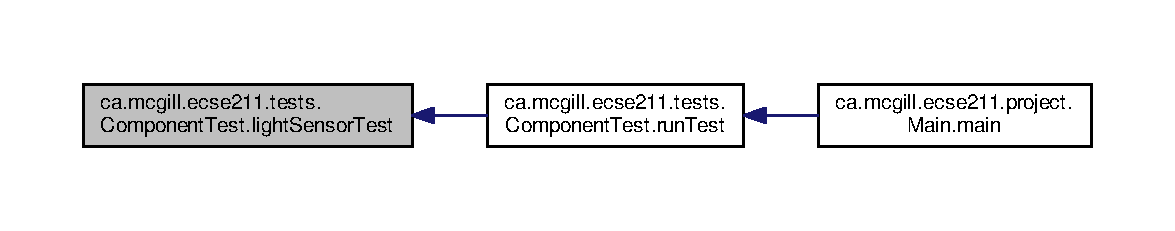
\includegraphics[width=350pt]{enumca_1_1mcgill_1_1ecse211_1_1tests_1_1_component_test_a3e8288f482b3806a0f3c4668951f3e36_icgraph}
\end{center}
\end{figure}
\mbox{\Hypertarget{enumca_1_1mcgill_1_1ecse211_1_1tests_1_1_component_test_ad11712dd74c5c64e84cd71186a59a087}\label{enumca_1_1mcgill_1_1ecse211_1_1tests_1_1_component_test_ad11712dd74c5c64e84cd71186a59a087}} 
\index{ca\+::mcgill\+::ecse211\+::tests\+::\+Component\+Test@{ca\+::mcgill\+::ecse211\+::tests\+::\+Component\+Test}!localization\+Test@{localization\+Test}}
\index{localization\+Test@{localization\+Test}!ca\+::mcgill\+::ecse211\+::tests\+::\+Component\+Test@{ca\+::mcgill\+::ecse211\+::tests\+::\+Component\+Test}}
\subsubsection{\texorpdfstring{localization\+Test()}{localizationTest()}}
{\footnotesize\ttfamily static void ca.\+mcgill.\+ecse211.\+tests.\+Component\+Test.\+localization\+Test (\begin{DoxyParamCaption}{ }\end{DoxyParamCaption}) throws \hyperlink{classca_1_1mcgill_1_1ecse211_1_1odometer_1_1_odometer_exceptions}{Odometer\+Exceptions}\hspace{0.3cm}{\ttfamily [static]}}

Test for localization\+Test


\begin{DoxyExceptions}{Exceptions}
{\em Odometer\+Exceptions} & \\
\hline
\end{DoxyExceptions}


Definition at line 92 of file Component\+Test.\+java.


\begin{DoxyCode}
92                                                                   \{
93     Navigation navigation = \textcolor{keyword}{new} Navigation(Game.leftMotor, Game.rightMotor);
94     UltrasonicLocalizer us = \textcolor{keyword}{new} UltrasonicLocalizer(navigation, Game.leftMotor, Game.rightMotor);
95     LightLocalizer lgLoc = \textcolor{keyword}{new} LightLocalizer(navigation, Game.leftMotor, Game.rightMotor);
96     us.localize(Button.ID\_LEFT);
97     lgLoc.localize(GameParameters.SC);
98   \}
\end{DoxyCode}
Here is the call graph for this function\+:\nopagebreak
\begin{figure}[H]
\begin{center}
\leavevmode
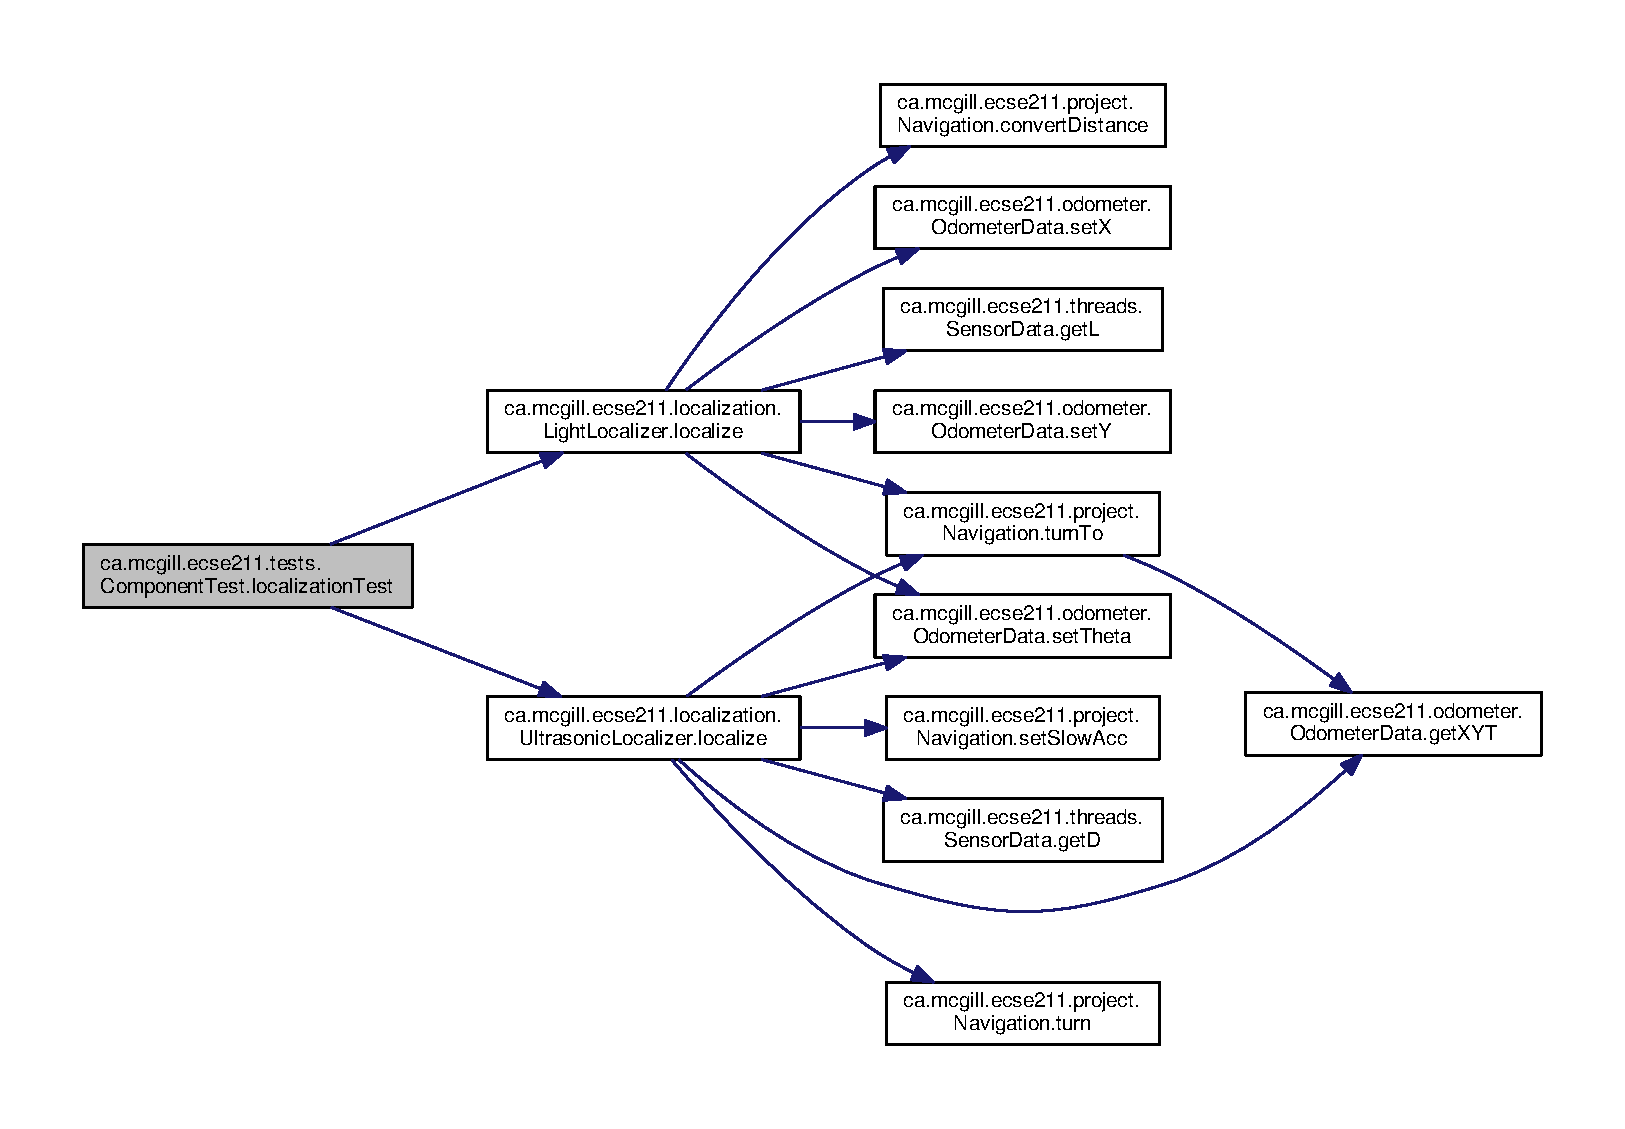
\includegraphics[width=350pt]{enumca_1_1mcgill_1_1ecse211_1_1tests_1_1_component_test_ad11712dd74c5c64e84cd71186a59a087_cgraph}
\end{center}
\end{figure}
Here is the caller graph for this function\+:\nopagebreak
\begin{figure}[H]
\begin{center}
\leavevmode
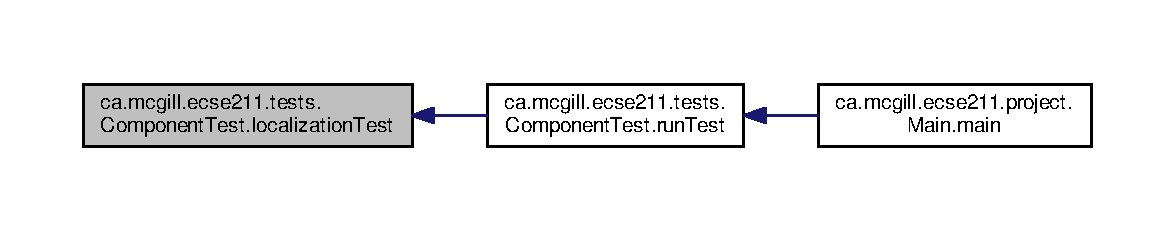
\includegraphics[width=350pt]{enumca_1_1mcgill_1_1ecse211_1_1tests_1_1_component_test_ad11712dd74c5c64e84cd71186a59a087_icgraph}
\end{center}
\end{figure}
\mbox{\Hypertarget{enumca_1_1mcgill_1_1ecse211_1_1tests_1_1_component_test_aa40592bb550b3526402faddbc0d890c7}\label{enumca_1_1mcgill_1_1ecse211_1_1tests_1_1_component_test_aa40592bb550b3526402faddbc0d890c7}} 
\index{ca\+::mcgill\+::ecse211\+::tests\+::\+Component\+Test@{ca\+::mcgill\+::ecse211\+::tests\+::\+Component\+Test}!navigation\+Test@{navigation\+Test}}
\index{navigation\+Test@{navigation\+Test}!ca\+::mcgill\+::ecse211\+::tests\+::\+Component\+Test@{ca\+::mcgill\+::ecse211\+::tests\+::\+Component\+Test}}
\subsubsection{\texorpdfstring{navigation\+Test()}{navigationTest()}}
{\footnotesize\ttfamily static void ca.\+mcgill.\+ecse211.\+tests.\+Component\+Test.\+navigation\+Test (\begin{DoxyParamCaption}{ }\end{DoxyParamCaption}) throws \hyperlink{classca_1_1mcgill_1_1ecse211_1_1odometer_1_1_odometer_exceptions}{Odometer\+Exceptions}\hspace{0.3cm}{\ttfamily [static]}}

Test for Navigation


\begin{DoxyExceptions}{Exceptions}
{\em Odometer\+Exceptions} & \\
\hline
\end{DoxyExceptions}


Definition at line 72 of file Component\+Test.\+java.


\begin{DoxyCode}
72                                                                 \{
73     Navigation nav = \textcolor{keyword}{new} Navigation(Game.leftMotor, Game.rightMotor);
74     nav.travelToWithCorrection(4, 2, \textcolor{keyword}{false});
75     nav.travelToWithCorrection(0, 0, \textcolor{keyword}{false});
76   \}
\end{DoxyCode}
Here is the call graph for this function\+:\nopagebreak
\begin{figure}[H]
\begin{center}
\leavevmode
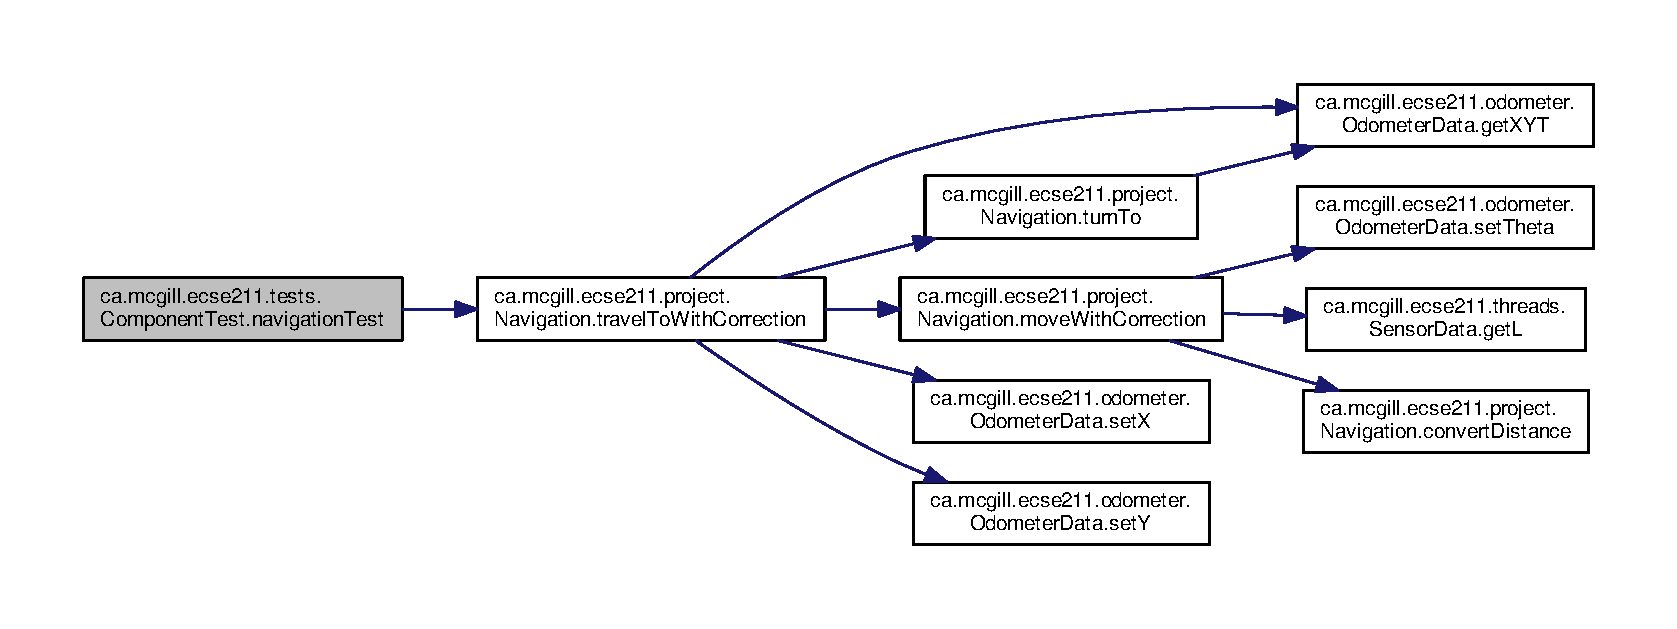
\includegraphics[width=350pt]{enumca_1_1mcgill_1_1ecse211_1_1tests_1_1_component_test_aa40592bb550b3526402faddbc0d890c7_cgraph}
\end{center}
\end{figure}
Here is the caller graph for this function\+:\nopagebreak
\begin{figure}[H]
\begin{center}
\leavevmode
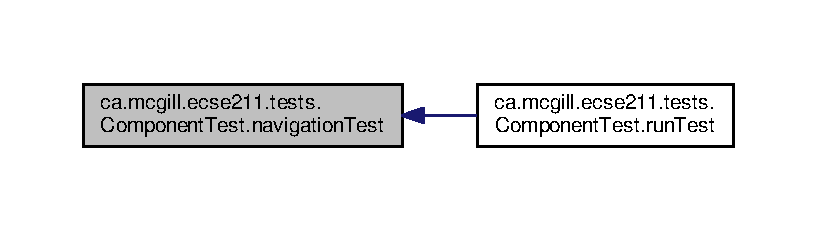
\includegraphics[width=350pt]{enumca_1_1mcgill_1_1ecse211_1_1tests_1_1_component_test_aa40592bb550b3526402faddbc0d890c7_icgraph}
\end{center}
\end{figure}
\mbox{\Hypertarget{enumca_1_1mcgill_1_1ecse211_1_1tests_1_1_component_test_a1ecca45b47067d825683cf46dcf22b62}\label{enumca_1_1mcgill_1_1ecse211_1_1tests_1_1_component_test_a1ecca45b47067d825683cf46dcf22b62}} 
\index{ca\+::mcgill\+::ecse211\+::tests\+::\+Component\+Test@{ca\+::mcgill\+::ecse211\+::tests\+::\+Component\+Test}!ring\+Motor\+Test@{ring\+Motor\+Test}}
\index{ring\+Motor\+Test@{ring\+Motor\+Test}!ca\+::mcgill\+::ecse211\+::tests\+::\+Component\+Test@{ca\+::mcgill\+::ecse211\+::tests\+::\+Component\+Test}}
\subsubsection{\texorpdfstring{ring\+Motor\+Test()}{ringMotorTest()}}
{\footnotesize\ttfamily static void ca.\+mcgill.\+ecse211.\+tests.\+Component\+Test.\+ring\+Motor\+Test (\begin{DoxyParamCaption}{ }\end{DoxyParamCaption}) throws \hyperlink{classca_1_1mcgill_1_1ecse211_1_1odometer_1_1_odometer_exceptions}{Odometer\+Exceptions}\hspace{0.3cm}{\ttfamily [static]}}

Test for ring detection


\begin{DoxyExceptions}{Exceptions}
{\em Odometer\+Exceptions} & \\
\hline
\end{DoxyExceptions}


Definition at line 119 of file Component\+Test.\+java.


\begin{DoxyCode}
119                                                                \{
120     Game.INSTANCE.usPoller.setStart(\textcolor{keyword}{false});
121     \textcolor{keyword}{final} RingSearcher searcher = \textcolor{keyword}{new} RingSearcher(Game.sensorMotor, Game.rodMotor);
122     Navigation navigation = \textcolor{keyword}{new} Navigation(Game.leftMotor, Game.rightMotor);
123     GameUtil.searchingFinder = \textcolor{keyword}{new} GameUtil.PathFinder(GameParameters.Island\_LL, GameParameters.Island\_UR);
124     GameUtil.startingFinder = \textcolor{keyword}{new} GameUtil.PathFinder(GameParameters.US\_LL, GameParameters.US\_UR);
125     Odometer.getOdometer().setXYT(1, 1, 0);
126     \textcolor{keywordtype}{int}[] tree = \{2,2\};
127     \textcolor{keywordtype}{int}[][] other = \{\{2,1\}, \{3,2\}, \{2,3\}, \{1,2\}\};
128     \textcolor{keywordflow}{for}(\textcolor{keywordtype}{int} i = 0; i < 4; i++) \{
129       navigation.travelToWithCorrection(other[i][0], other[i][1],\textcolor{keyword}{false});
130       navigation.turn(-90);
131       \textcolor{comment}{//navigation.searchRingSet(searcher);}
132     \}
133   \}
\end{DoxyCode}
Here is the call graph for this function\+:
\nopagebreak
\begin{figure}[H]
\begin{center}
\leavevmode
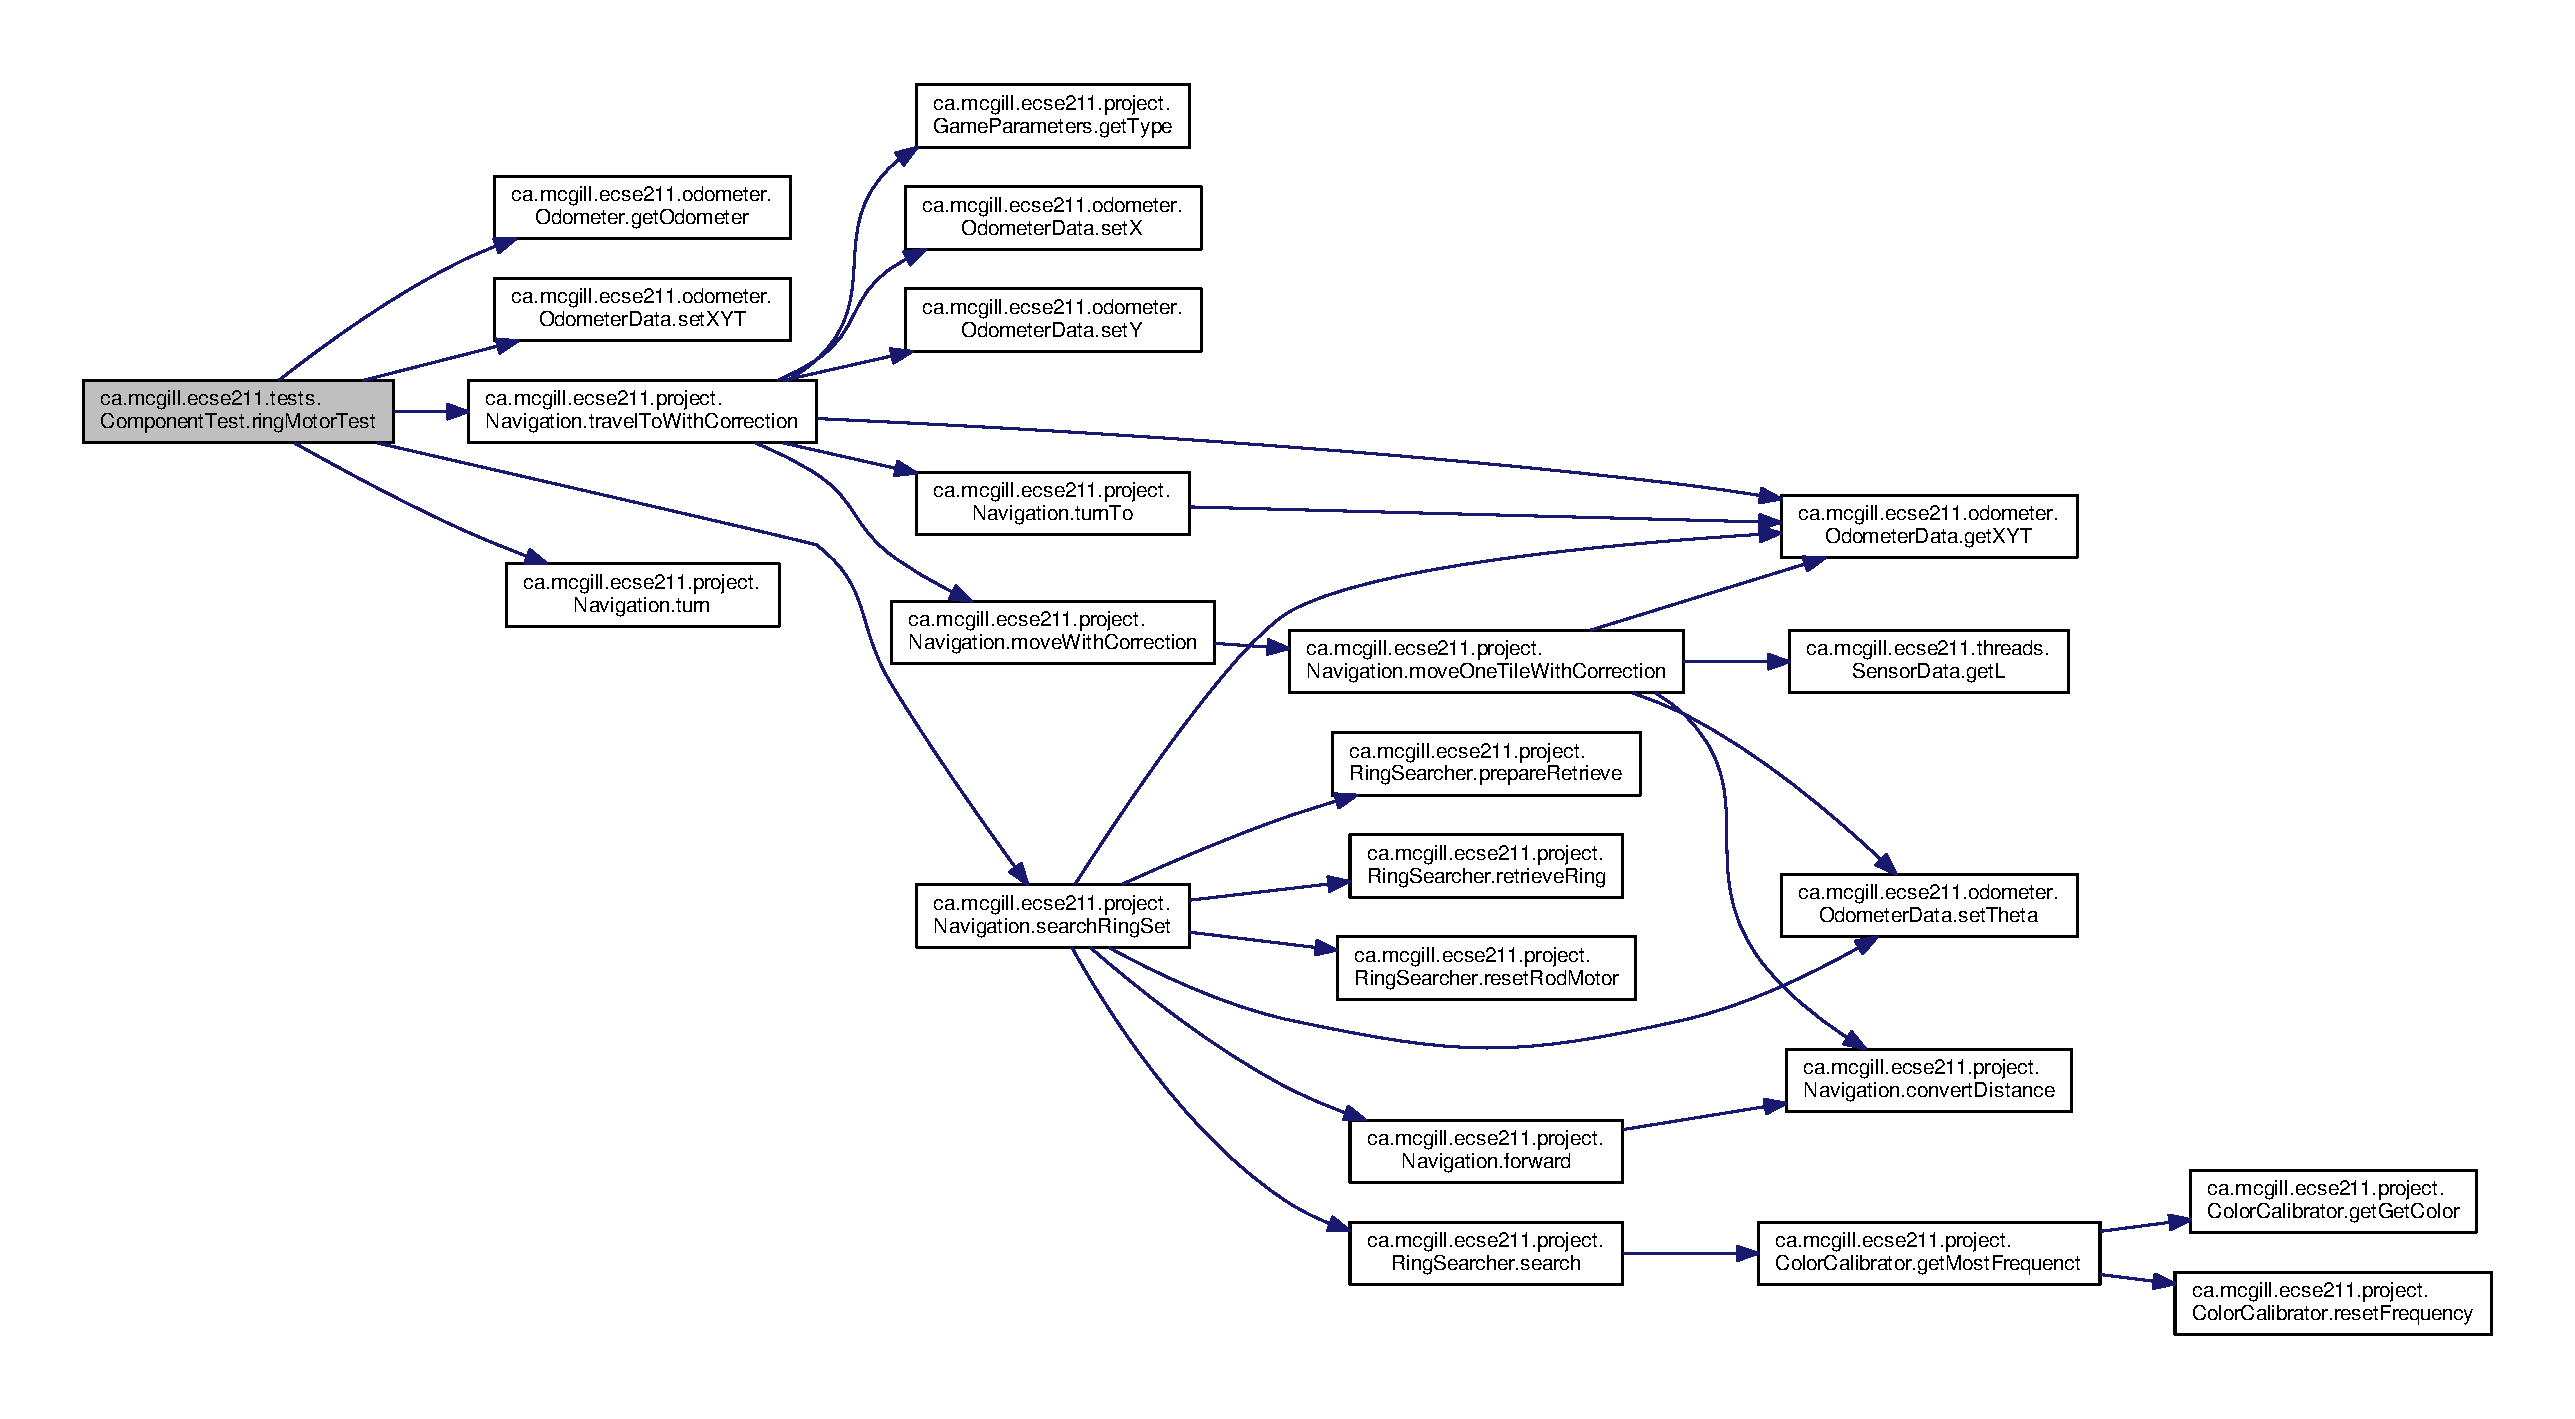
\includegraphics[width=350pt]{enumca_1_1mcgill_1_1ecse211_1_1tests_1_1_component_test_a1ecca45b47067d825683cf46dcf22b62_cgraph}
\end{center}
\end{figure}
Here is the caller graph for this function\+:
\nopagebreak
\begin{figure}[H]
\begin{center}
\leavevmode
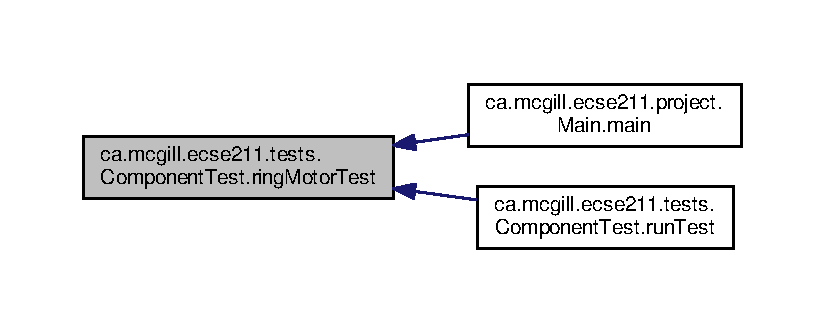
\includegraphics[width=350pt]{enumca_1_1mcgill_1_1ecse211_1_1tests_1_1_component_test_a1ecca45b47067d825683cf46dcf22b62_icgraph}
\end{center}
\end{figure}
\mbox{\Hypertarget{enumca_1_1mcgill_1_1ecse211_1_1tests_1_1_component_test_a5dc8bf97bc48adf5bee88d425a1a974e}\label{enumca_1_1mcgill_1_1ecse211_1_1tests_1_1_component_test_a5dc8bf97bc48adf5bee88d425a1a974e}} 
\index{ca\+::mcgill\+::ecse211\+::tests\+::\+Component\+Test@{ca\+::mcgill\+::ecse211\+::tests\+::\+Component\+Test}!run\+Test@{run\+Test}}
\index{run\+Test@{run\+Test}!ca\+::mcgill\+::ecse211\+::tests\+::\+Component\+Test@{ca\+::mcgill\+::ecse211\+::tests\+::\+Component\+Test}}
\subsubsection{\texorpdfstring{run\+Test()}{runTest()}}
{\footnotesize\ttfamily static void ca.\+mcgill.\+ecse211.\+tests.\+Component\+Test.\+run\+Test (\begin{DoxyParamCaption}\item[{\hyperlink{enumca_1_1mcgill_1_1ecse211_1_1tests_1_1_component_test_1_1_type}{Type}}]{test\+Type }\end{DoxyParamCaption}) throws Exception\hspace{0.3cm}{\ttfamily [static]}}

This method selects test for each individual components of the design


\begin{DoxyParams}{Parameters}
{\em type} & \\
\hline
\end{DoxyParams}

\begin{DoxyExceptions}{Exceptions}
{\em Exception} & \\
\hline
\end{DoxyExceptions}


Definition at line 40 of file Component\+Test.\+java.


\begin{DoxyCode}
40                                                              \{
41     \textcolor{keywordflow}{try} \{
42       \textcolor{keywordflow}{switch} (testType) \{
43         \textcolor{keywordflow}{case} Navigation:
44           ComponentTest.navigationTest();
45           \textcolor{keywordflow}{break};
46         \textcolor{keywordflow}{case} Localization:
47           ComponentTest.localizationTest();
48           \textcolor{keywordflow}{break};
49         \textcolor{keywordflow}{case} UltrasonicSensor:
50           ComponentTest.ultrasonicSensorTest();
51           \textcolor{keywordflow}{break};
52         \textcolor{keywordflow}{case} LightSensor:
53           ComponentTest.lightSensorTest();
54           \textcolor{keywordflow}{break};
55         \textcolor{keywordflow}{case} RingDetection:
56           ComponentTest.ringMotorTest();
57           \textcolor{keywordflow}{break};
58         \textcolor{keywordflow}{default}:
59           System.out.println(\textcolor{stringliteral}{"Invalid test type selected"});
60           \textcolor{keywordflow}{break};
61       \}
62     \} \textcolor{keywordflow}{catch} (Exception e) \{
63       \textcolor{keywordflow}{throw} e;
64     \}
65   \}
\end{DoxyCode}
Here is the call graph for this function\+:
\nopagebreak
\begin{figure}[H]
\begin{center}
\leavevmode
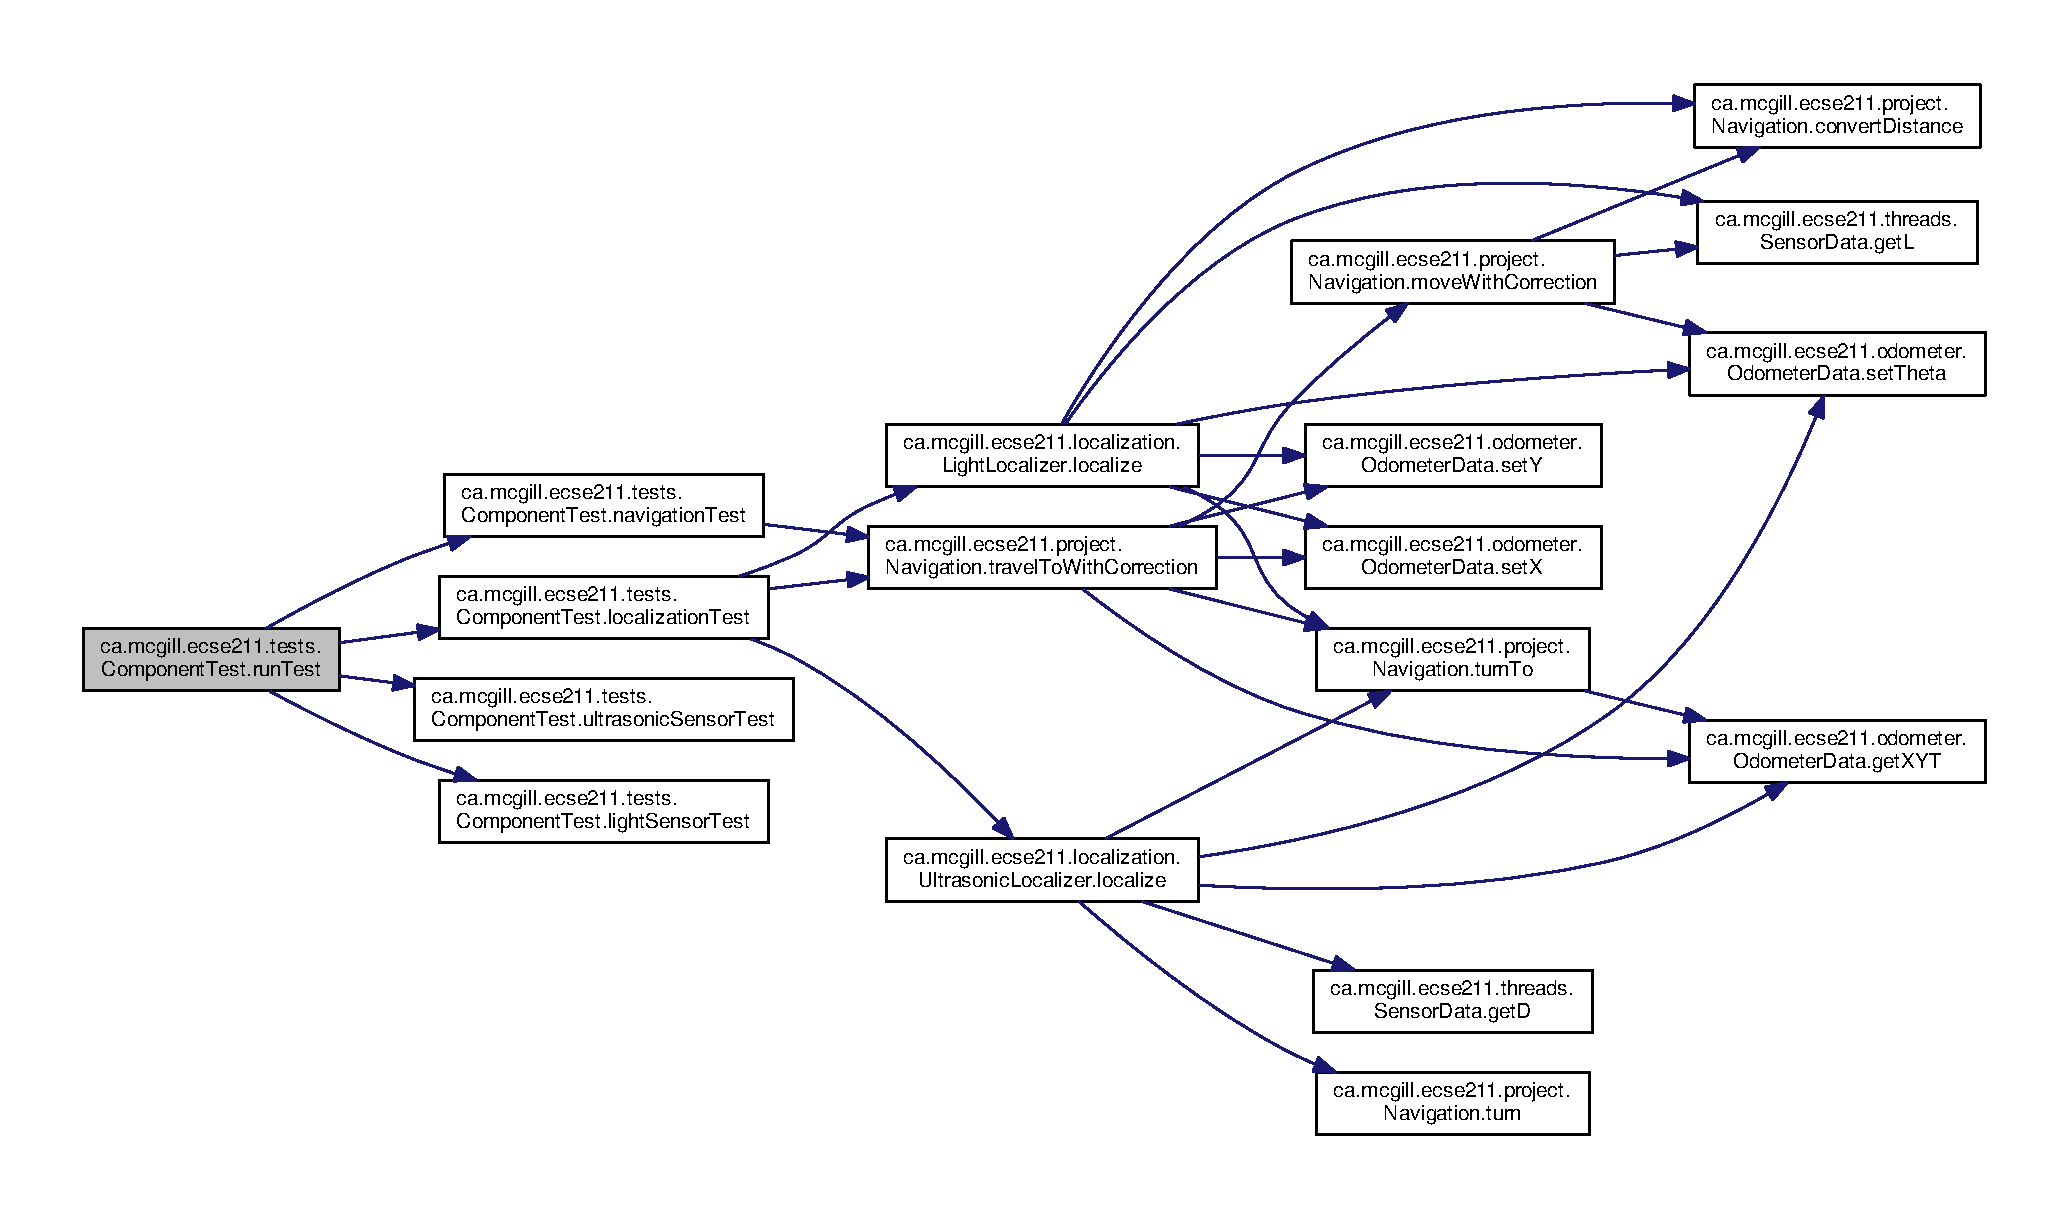
\includegraphics[width=350pt]{enumca_1_1mcgill_1_1ecse211_1_1tests_1_1_component_test_a5dc8bf97bc48adf5bee88d425a1a974e_cgraph}
\end{center}
\end{figure}
\mbox{\Hypertarget{enumca_1_1mcgill_1_1ecse211_1_1tests_1_1_component_test_ae85caa20c6391bacc4fdbd411ee3f113}\label{enumca_1_1mcgill_1_1ecse211_1_1tests_1_1_component_test_ae85caa20c6391bacc4fdbd411ee3f113}} 
\index{ca\+::mcgill\+::ecse211\+::tests\+::\+Component\+Test@{ca\+::mcgill\+::ecse211\+::tests\+::\+Component\+Test}!tunnel\+Test@{tunnel\+Test}}
\index{tunnel\+Test@{tunnel\+Test}!ca\+::mcgill\+::ecse211\+::tests\+::\+Component\+Test@{ca\+::mcgill\+::ecse211\+::tests\+::\+Component\+Test}}
\subsubsection{\texorpdfstring{tunnel\+Test()}{tunnelTest()}}
{\footnotesize\ttfamily static void ca.\+mcgill.\+ecse211.\+tests.\+Component\+Test.\+tunnel\+Test (\begin{DoxyParamCaption}{ }\end{DoxyParamCaption}) throws Exception\hspace{0.3cm}{\ttfamily [static]}}



Definition at line 78 of file Component\+Test.\+java.


\begin{DoxyCode}
78                                                    \{
79     Navigation navigation = \textcolor{keyword}{new} Navigation(Game.leftMotor, Game.rightMotor);
80     GameUtil.searchingFinder = \textcolor{keyword}{new} GameUtil.PathFinder(GameParameters.Island\_LL, GameParameters.Island\_UR);
81     GameUtil.startingFinder = \textcolor{keyword}{new} GameUtil.PathFinder(GameParameters.US\_LL, GameParameters.US\_UR);
82     Odometer.getOdometer().setXYT(1, 7, 90);
83     navigation.goThroughTunnel();
84     navigation.goThroughTunnel();
85   \}
\end{DoxyCode}
Here is the call graph for this function\+:
\nopagebreak
\begin{figure}[H]
\begin{center}
\leavevmode
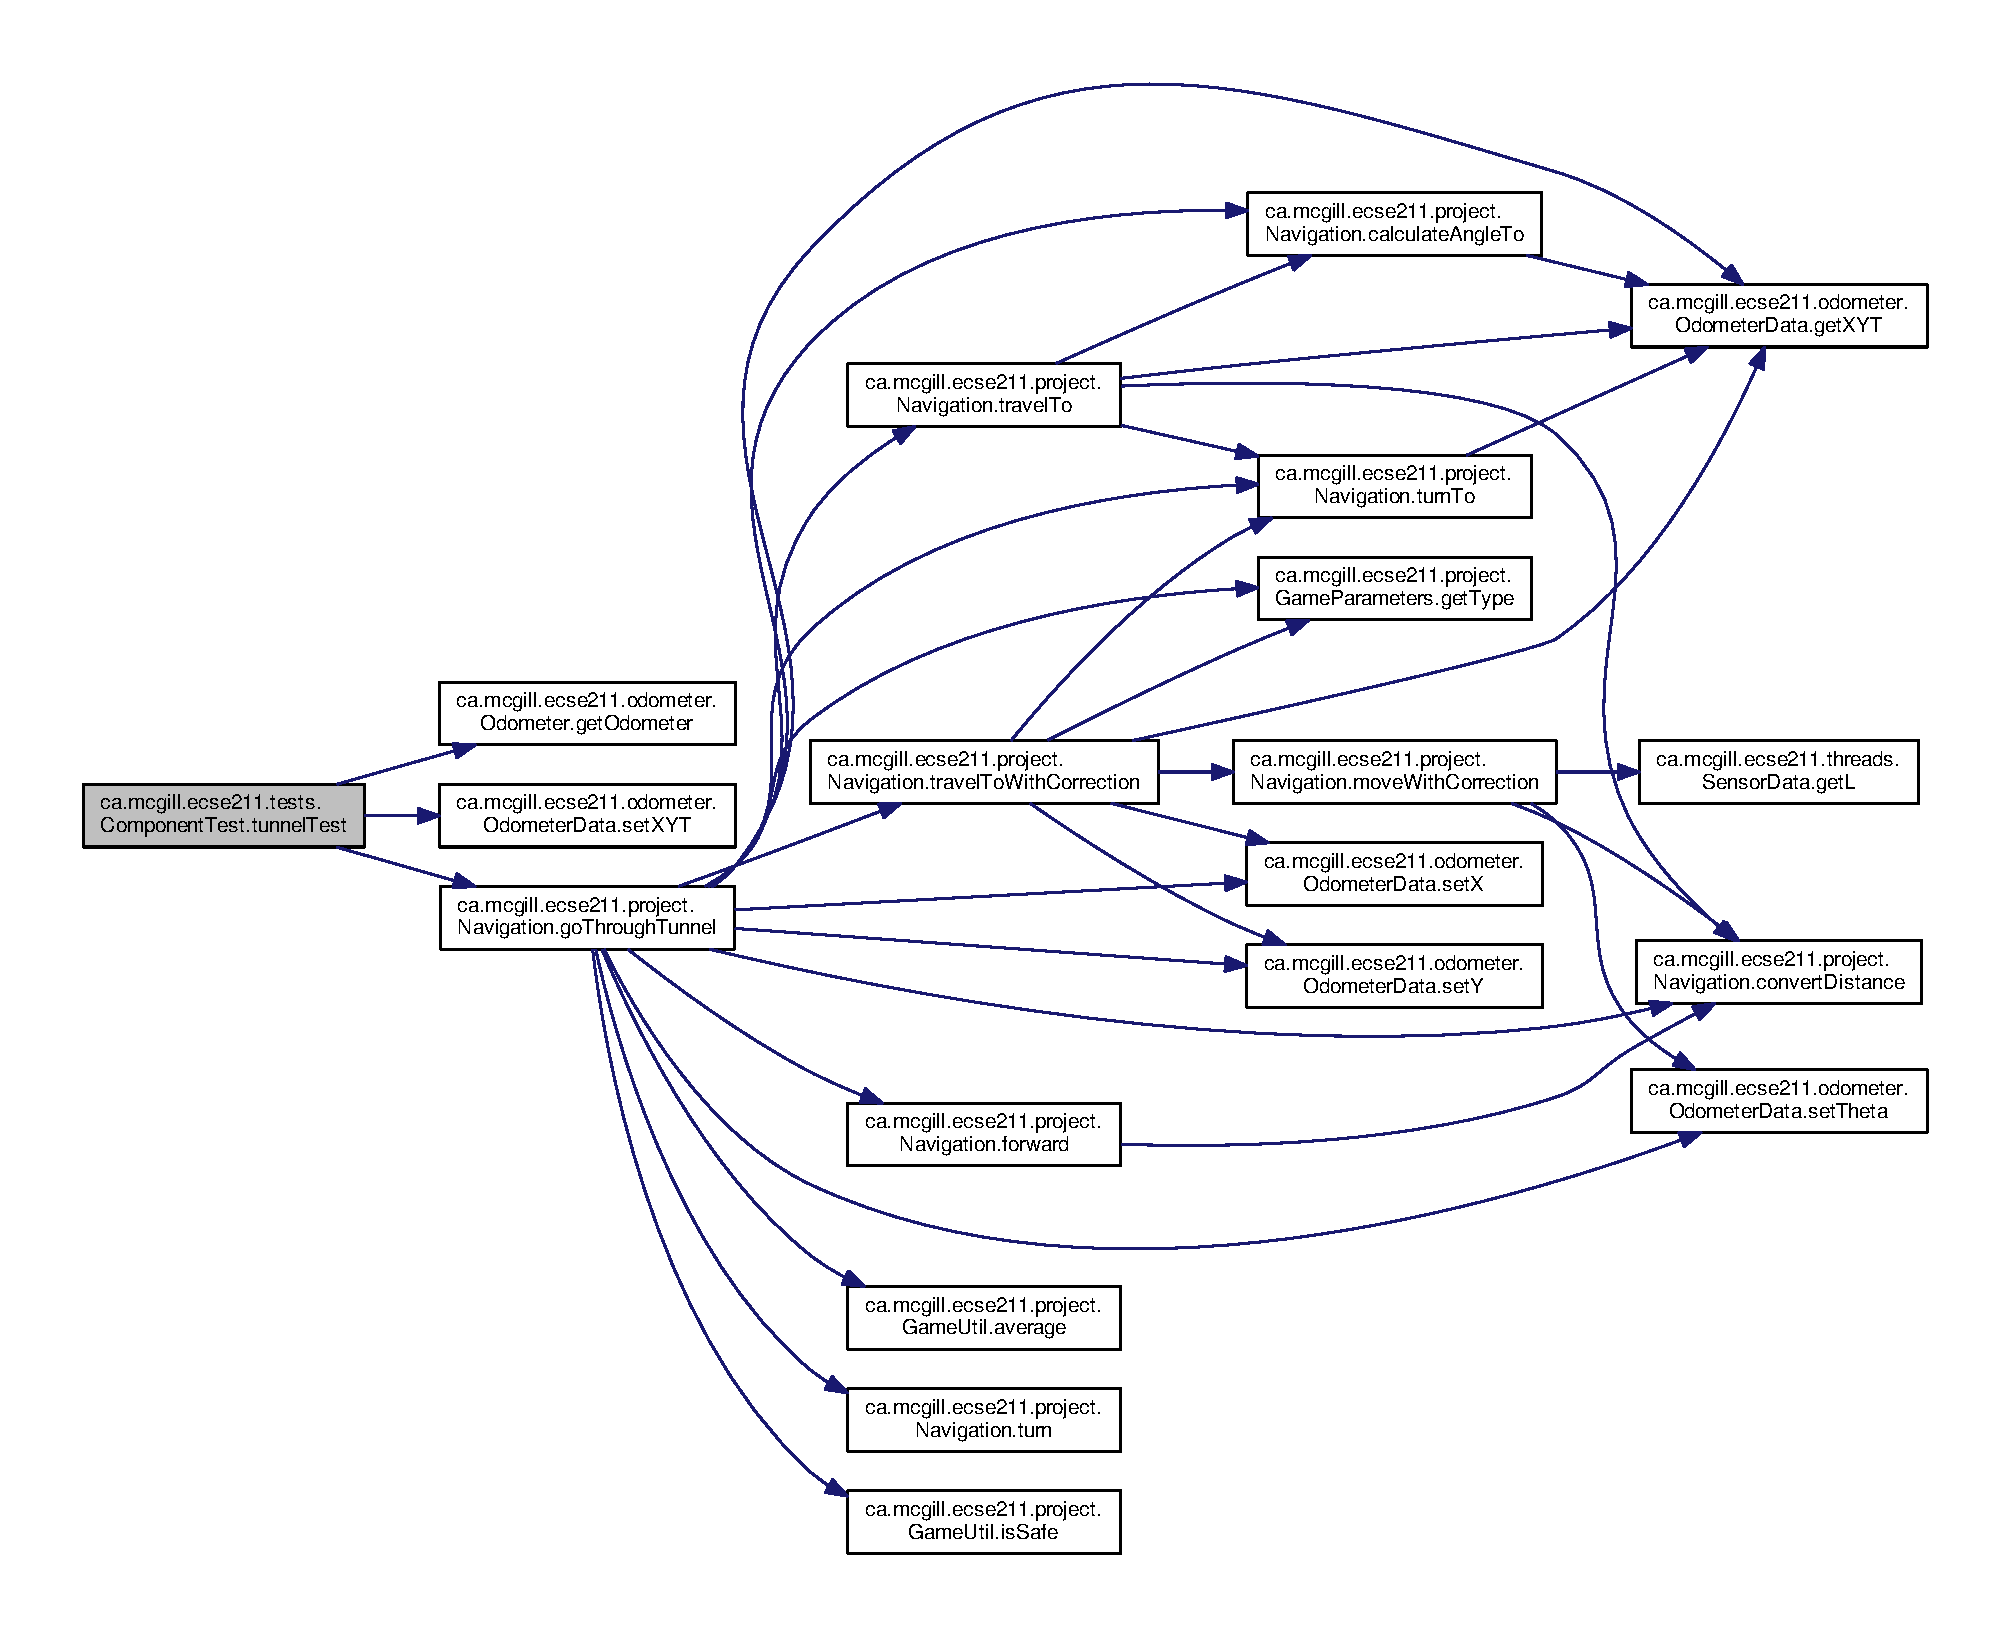
\includegraphics[width=350pt]{enumca_1_1mcgill_1_1ecse211_1_1tests_1_1_component_test_ae85caa20c6391bacc4fdbd411ee3f113_cgraph}
\end{center}
\end{figure}
\mbox{\Hypertarget{enumca_1_1mcgill_1_1ecse211_1_1tests_1_1_component_test_a05cd9d95458b11ed57ca001a28fffa7c}\label{enumca_1_1mcgill_1_1ecse211_1_1tests_1_1_component_test_a05cd9d95458b11ed57ca001a28fffa7c}} 
\index{ca\+::mcgill\+::ecse211\+::tests\+::\+Component\+Test@{ca\+::mcgill\+::ecse211\+::tests\+::\+Component\+Test}!ultrasonic\+Sensor\+Test@{ultrasonic\+Sensor\+Test}}
\index{ultrasonic\+Sensor\+Test@{ultrasonic\+Sensor\+Test}!ca\+::mcgill\+::ecse211\+::tests\+::\+Component\+Test@{ca\+::mcgill\+::ecse211\+::tests\+::\+Component\+Test}}
\subsubsection{\texorpdfstring{ultrasonic\+Sensor\+Test()}{ultrasonicSensorTest()}}
{\footnotesize\ttfamily static void ca.\+mcgill.\+ecse211.\+tests.\+Component\+Test.\+ultrasonic\+Sensor\+Test (\begin{DoxyParamCaption}{ }\end{DoxyParamCaption})\hspace{0.3cm}{\ttfamily [static]}}

Test for Ultrasonic\+Sensor 

Definition at line 103 of file Component\+Test.\+java.


\begin{DoxyCode}
103                                             \{
104 
105   \}
\end{DoxyCode}
Here is the caller graph for this function\+:
\nopagebreak
\begin{figure}[H]
\begin{center}
\leavevmode
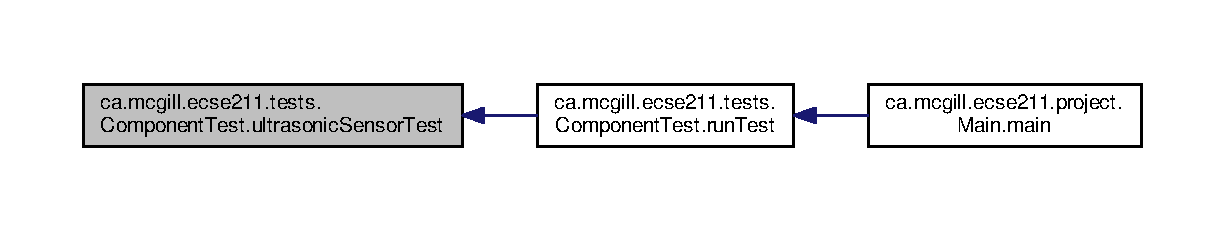
\includegraphics[width=350pt]{enumca_1_1mcgill_1_1ecse211_1_1tests_1_1_component_test_a05cd9d95458b11ed57ca001a28fffa7c_icgraph}
\end{center}
\end{figure}


The documentation for this enum was generated from the following file\+:\begin{DoxyCompactItemize}
\item 
/home/ccc/\+Final\+Project/src/ca/mcgill/ecse211/tests/\hyperlink{_component_test_8java}{Component\+Test.\+java}\end{DoxyCompactItemize}

\hypertarget{classca_1_1mcgill_1_1ecse211_1_1project_1_1_display}{}\section{ca.\+mcgill.\+ecse211.\+project.\+Display Class Reference}
\label{classca_1_1mcgill_1_1ecse211_1_1project_1_1_display}\index{ca.\+mcgill.\+ecse211.\+project.\+Display@{ca.\+mcgill.\+ecse211.\+project.\+Display}}


Inheritance diagram for ca.\+mcgill.\+ecse211.\+project.\+Display\+:\nopagebreak
\begin{figure}[H]
\begin{center}
\leavevmode
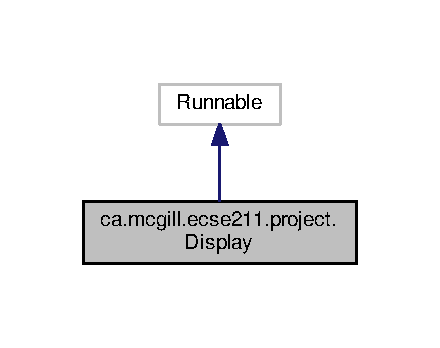
\includegraphics[width=211pt]{classca_1_1mcgill_1_1ecse211_1_1project_1_1_display__inherit__graph}
\end{center}
\end{figure}


Collaboration diagram for ca.\+mcgill.\+ecse211.\+project.\+Display\+:\nopagebreak
\begin{figure}[H]
\begin{center}
\leavevmode
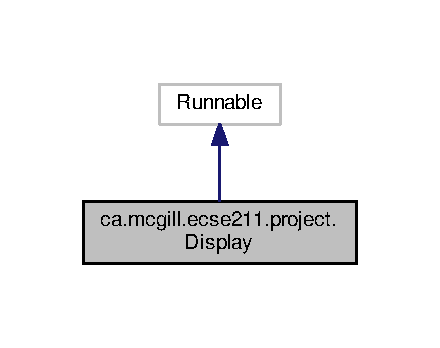
\includegraphics[width=211pt]{classca_1_1mcgill_1_1ecse211_1_1project_1_1_display__coll__graph}
\end{center}
\end{figure}
\subsection*{Public Member Functions}
\begin{DoxyCompactItemize}
\item 
\hyperlink{classca_1_1mcgill_1_1ecse211_1_1project_1_1_display_af0970123ca090749bfb2f5b9f478c01d}{Display} (Text\+L\+CD lcd)  throws Odometer\+Exceptions 
\item 
\hyperlink{classca_1_1mcgill_1_1ecse211_1_1project_1_1_display_a690cd91bcc8024950c2b8e3b2613c801}{Display} (Text\+L\+CD lcd, long timeout)  throws Odometer\+Exceptions 
\item 
void \hyperlink{classca_1_1mcgill_1_1ecse211_1_1project_1_1_display_ab508a8bc2b738499bec2c432a814cba5}{run} ()
\end{DoxyCompactItemize}


\subsection{Detailed Description}
This class is used to display the content of the odometer variables (x, y, Theta)

\begin{DoxyAuthor}{Author}
Caspar Cedro 

Percy Chen 

Patrick Erath 

Anssam Ghezala 

Susan Matuszewski 

Kamy Moussavi Kafi 
\end{DoxyAuthor}


Definition at line 19 of file Display.\+java.



\subsection{Constructor \& Destructor Documentation}
\mbox{\Hypertarget{classca_1_1mcgill_1_1ecse211_1_1project_1_1_display_af0970123ca090749bfb2f5b9f478c01d}\label{classca_1_1mcgill_1_1ecse211_1_1project_1_1_display_af0970123ca090749bfb2f5b9f478c01d}} 
\index{ca\+::mcgill\+::ecse211\+::project\+::\+Display@{ca\+::mcgill\+::ecse211\+::project\+::\+Display}!Display@{Display}}
\index{Display@{Display}!ca\+::mcgill\+::ecse211\+::project\+::\+Display@{ca\+::mcgill\+::ecse211\+::project\+::\+Display}}
\subsubsection{\texorpdfstring{Display()}{Display()}\hspace{0.1cm}{\footnotesize\ttfamily [1/2]}}
{\footnotesize\ttfamily ca.\+mcgill.\+ecse211.\+project.\+Display.\+Display (\begin{DoxyParamCaption}\item[{Text\+L\+CD}]{lcd }\end{DoxyParamCaption}) throws \hyperlink{classca_1_1mcgill_1_1ecse211_1_1odometer_1_1_odometer_exceptions}{Odometer\+Exceptions}}

This is the class constructor for a display object that controls an E\+V3 brick display


\begin{DoxyParams}{Parameters}
{\em lcd} & A Text\+L\+CD object instance to control \\
\hline
\end{DoxyParams}

\begin{DoxyExceptions}{Exceptions}
{\em Odometer\+Exceptions} & \\
\hline
\end{DoxyExceptions}


Definition at line 35 of file Display.\+java.


\begin{DoxyCode}
35                                                         \{
36     this.odo = Odometer.\hyperlink{classca_1_1mcgill_1_1ecse211_1_1odometer_1_1_odometer_a99171f11e34dea918fa9dd069d721439}{getOdometer}();
37     this.sensdata = SensorData.\hyperlink{classca_1_1mcgill_1_1ecse211_1_1threads_1_1_sensor_data_a8260aba53b4474ca1275e4ce26157977}{getSensorData}();
38     this.lcd = lcd;
39   \}
\end{DoxyCode}
Here is the call graph for this function\+:\nopagebreak
\begin{figure}[H]
\begin{center}
\leavevmode
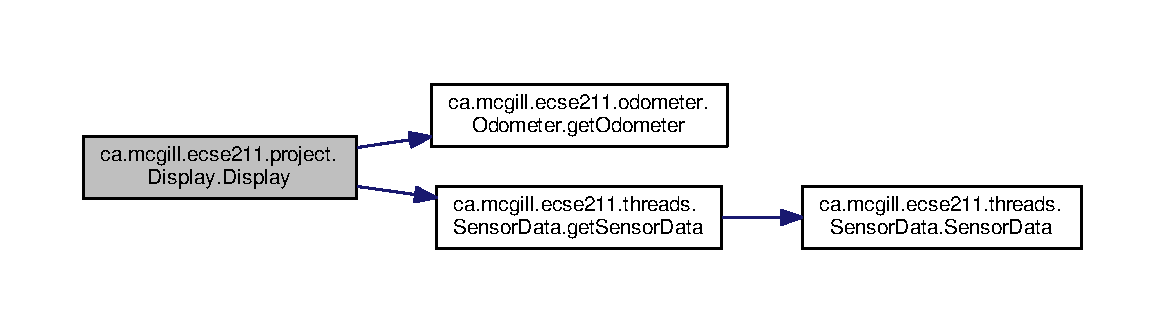
\includegraphics[width=350pt]{classca_1_1mcgill_1_1ecse211_1_1project_1_1_display_af0970123ca090749bfb2f5b9f478c01d_cgraph}
\end{center}
\end{figure}
\mbox{\Hypertarget{classca_1_1mcgill_1_1ecse211_1_1project_1_1_display_a690cd91bcc8024950c2b8e3b2613c801}\label{classca_1_1mcgill_1_1ecse211_1_1project_1_1_display_a690cd91bcc8024950c2b8e3b2613c801}} 
\index{ca\+::mcgill\+::ecse211\+::project\+::\+Display@{ca\+::mcgill\+::ecse211\+::project\+::\+Display}!Display@{Display}}
\index{Display@{Display}!ca\+::mcgill\+::ecse211\+::project\+::\+Display@{ca\+::mcgill\+::ecse211\+::project\+::\+Display}}
\subsubsection{\texorpdfstring{Display()}{Display()}\hspace{0.1cm}{\footnotesize\ttfamily [2/2]}}
{\footnotesize\ttfamily ca.\+mcgill.\+ecse211.\+project.\+Display.\+Display (\begin{DoxyParamCaption}\item[{Text\+L\+CD}]{lcd,  }\item[{long}]{timeout }\end{DoxyParamCaption}) throws \hyperlink{classca_1_1mcgill_1_1ecse211_1_1odometer_1_1_odometer_exceptions}{Odometer\+Exceptions}}

This is the overloaded class constructor for a display object


\begin{DoxyParams}{Parameters}
{\em lcd} & A Text\+L\+CD object instance to control \\
\hline
{\em timeout} & A duration of time to update the display for \\
\hline
\end{DoxyParams}

\begin{DoxyExceptions}{Exceptions}
{\em Odometer\+Exceptions} & \\
\hline
\end{DoxyExceptions}


Definition at line 48 of file Display.\+java.


\begin{DoxyCode}
48                                                                       \{
49     odo = Odometer.\hyperlink{classca_1_1mcgill_1_1ecse211_1_1odometer_1_1_odometer_a99171f11e34dea918fa9dd069d721439}{getOdometer}();
50     this.timeout = timeout;
51     this.lcd = lcd;
52   \}
\end{DoxyCode}
Here is the call graph for this function\+:\nopagebreak
\begin{figure}[H]
\begin{center}
\leavevmode
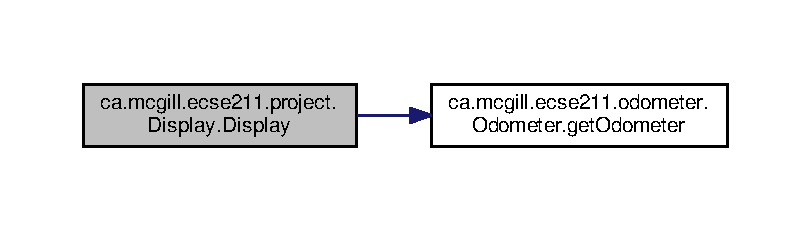
\includegraphics[width=350pt]{classca_1_1mcgill_1_1ecse211_1_1project_1_1_display_a690cd91bcc8024950c2b8e3b2613c801_cgraph}
\end{center}
\end{figure}


\subsection{Member Function Documentation}
\mbox{\Hypertarget{classca_1_1mcgill_1_1ecse211_1_1project_1_1_display_ab508a8bc2b738499bec2c432a814cba5}\label{classca_1_1mcgill_1_1ecse211_1_1project_1_1_display_ab508a8bc2b738499bec2c432a814cba5}} 
\index{ca\+::mcgill\+::ecse211\+::project\+::\+Display@{ca\+::mcgill\+::ecse211\+::project\+::\+Display}!run@{run}}
\index{run@{run}!ca\+::mcgill\+::ecse211\+::project\+::\+Display@{ca\+::mcgill\+::ecse211\+::project\+::\+Display}}
\subsubsection{\texorpdfstring{run()}{run()}}
{\footnotesize\ttfamily void ca.\+mcgill.\+ecse211.\+project.\+Display.\+run (\begin{DoxyParamCaption}{ }\end{DoxyParamCaption})}

This method is called when the \hyperlink{classca_1_1mcgill_1_1ecse211_1_1project_1_1_display}{Display} thread is started. 

Definition at line 57 of file Display.\+java.


\begin{DoxyCode}
57                     \{
58     lcd.clear();
59 
60     \textcolor{keywordtype}{long} updateStart, updateEnd;
61 
62     \textcolor{keywordtype}{long} tStart = System.currentTimeMillis();
63 
64     \textcolor{keywordflow}{do} \{
65       updateStart = System.currentTimeMillis();
66 
67       \textcolor{comment}{// Retrieve x, y and Theta information}
68       position = odo.\hyperlink{classca_1_1mcgill_1_1ecse211_1_1odometer_1_1_odometer_data_a8f40f0264c68f0cbed4fff1723ae7863}{getXYT}();
69       rgb = sensdata.\hyperlink{classca_1_1mcgill_1_1ecse211_1_1threads_1_1_sensor_data_a76313564e284f5cdb66aefce4e595f3b}{getRGB}();
70 
71       \textcolor{comment}{// Print x,y, and theta information}
72       DecimalFormat numberFormat = \textcolor{keyword}{new} DecimalFormat(\textcolor{stringliteral}{"######0.00"});
73       \textcolor{comment}{// The last two parameters to lcd.drawString denote the x and y coordinate to draw at.}
74    \textcolor{comment}{//   lcd.drawString("X: " + numberFormat.format(position[0]), 0, 0);}
75    \textcolor{comment}{//   lcd.drawString("Y: " + numberFormat.format(position[1]), 0, 1);}
76   \textcolor{comment}{//    lcd.drawString("T: " + numberFormat.format(position[2]), 0, 2);}
77 \textcolor{comment}{//      lcd.drawString("LL: " + numberFormat.format(sensdata.getL()[0]), 0, 3);}
78 \textcolor{comment}{//      lcd.drawString("LR: " + numberFormat.format(sensdata.getL()[1]), 0, 4);}
79 \textcolor{comment}{//      lcd.drawString("D: " + numberFormat.format(sensdata.getD()), 0, 5);}
80 
81       lcd.drawString(String.format(\textcolor{stringliteral}{"(R: %d G: %d B: %d)"}, (\textcolor{keywordtype}{int}) rgb[0], (\textcolor{keywordtype}{int}) rgb[1], (\textcolor{keywordtype}{int}) rgb[2]),
82           0, 4);
83 \textcolor{comment}{//      if (ColorCalibrator.getColor((int) rgb[0], (int) rgb[1],}
84 \textcolor{comment}{//          (int) rgb[2]) != ColorCalibrator.Color.Other) \{}
85 \textcolor{comment}{//        lcd.drawString("Object Detected", 0, 5);}
86 \textcolor{comment}{//      \} else \{}
87 \textcolor{comment}{//        // Draw whitespace on our display}
88 \textcolor{comment}{//        lcd.drawString("                   ", 0, 5);}
89 \textcolor{comment}{//      \}}
90 
91       lcd.drawString(String.format(\textcolor{stringliteral}{"%1$-10s"}, ColorCalibrator.getColor().toString()), 0, 6);
92       lcd.drawString(\textcolor{stringliteral}{"A:"} + numberFormat.format(sensdata.\hyperlink{classca_1_1mcgill_1_1ecse211_1_1threads_1_1_sensor_data_acc8f6cc56f39c8ea6b812cd8b135eca6}{getA}()), 0, 7);
93 
94 \textcolor{comment}{//       lcd.drawString(String.format("(r: %d", (int)rgb[0]), 0, 3);}
95 \textcolor{comment}{//       lcd.drawString(String.format("(g: %d", (int)rgb[1]), 0, 4);}
96 \textcolor{comment}{//       lcd.drawString(String.format("(b: %d", (int)rgb[2]), 0, 5);}
97 
98       \textcolor{comment}{// This ensures that the data is updated only once every period}
99       updateEnd = System.currentTimeMillis();
100       \textcolor{keywordflow}{if} (updateEnd - updateStart < DISPLAY\_PERIOD) \{
101         \textcolor{keywordflow}{try} \{
102           Thread.sleep(DISPLAY\_PERIOD - (updateEnd - updateStart));
103         \} \textcolor{keywordflow}{catch} (InterruptedException e) \{
104           e.printStackTrace();
105         \}
106       \}
107     \} \textcolor{keywordflow}{while} ((updateEnd - tStart) <= timeout);
108   \}
\end{DoxyCode}
Here is the call graph for this function\+:\nopagebreak
\begin{figure}[H]
\begin{center}
\leavevmode
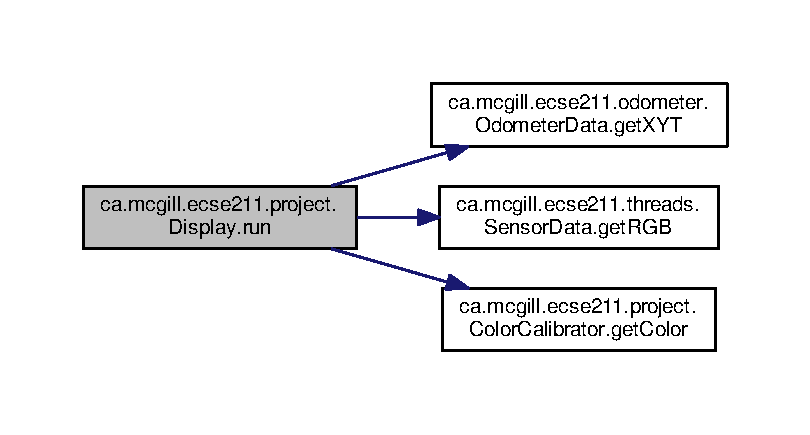
\includegraphics[width=350pt]{classca_1_1mcgill_1_1ecse211_1_1project_1_1_display_ab508a8bc2b738499bec2c432a814cba5_cgraph}
\end{center}
\end{figure}


The documentation for this class was generated from the following file\+:\begin{DoxyCompactItemize}
\item 
/home/ccc/\+Final\+Project/src/ca/mcgill/ecse211/project/\hyperlink{_display_8java}{Display.\+java}\end{DoxyCompactItemize}

\hypertarget{enumca_1_1mcgill_1_1ecse211_1_1project_1_1_game}{}\section{ca.\+mcgill.\+ecse211.\+project.\+Game Enum Reference}
\label{enumca_1_1mcgill_1_1ecse211_1_1project_1_1_game}\index{ca.\+mcgill.\+ecse211.\+project.\+Game@{ca.\+mcgill.\+ecse211.\+project.\+Game}}


Collaboration diagram for ca.\+mcgill.\+ecse211.\+project.\+Game\+:\nopagebreak
\begin{figure}[H]
\begin{center}
\leavevmode
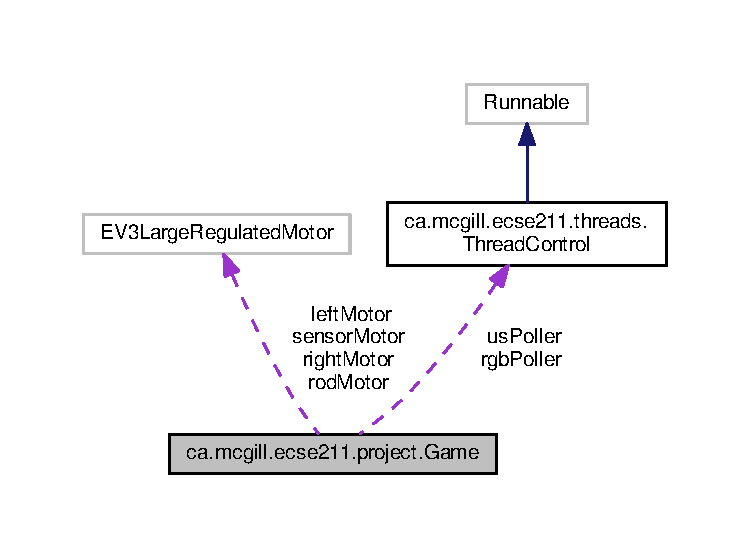
\includegraphics[width=350pt]{enumca_1_1mcgill_1_1ecse211_1_1project_1_1_game__coll__graph}
\end{center}
\end{figure}
\subsection*{Classes}
\begin{DoxyCompactItemize}
\item 
enum \hyperlink{enumca_1_1mcgill_1_1ecse211_1_1project_1_1_game_1_1_status}{Status}
\end{DoxyCompactItemize}
\subsection*{Public Member Functions}
\begin{DoxyCompactItemize}
\item 
String \hyperlink{enumca_1_1mcgill_1_1ecse211_1_1project_1_1_game_a43a5763d183e0bcacd402c872c07273e}{get\+Status\+Full\+Name} ()
\item 
\hyperlink{enumca_1_1mcgill_1_1ecse211_1_1project_1_1_game_1_1_status}{Status} \hyperlink{enumca_1_1mcgill_1_1ecse211_1_1project_1_1_game_a620374b3eeb3dd7e0abd26f3ced9053b}{get\+Status} ()
\item 
boolean \hyperlink{enumca_1_1mcgill_1_1ecse211_1_1project_1_1_game_a5b304a6a59ddee3f8c7d37bba8a4c129}{ready} (\hyperlink{classca_1_1mcgill_1_1ecse211_1_1localization_1_1_ultrasonic_localizer}{Ultrasonic\+Localizer} us, \hyperlink{classca_1_1mcgill_1_1ecse211_1_1localization_1_1_light_localizer}{Light\+Localizer} lg\+Loc)
\item 
boolean \hyperlink{enumca_1_1mcgill_1_1ecse211_1_1project_1_1_game_ad3d03cffa33c927317d8fcba0c928a24}{navigate\+To\+Tunnel} (\hyperlink{classca_1_1mcgill_1_1ecse211_1_1project_1_1_navigation}{Navigation} navigation, \hyperlink{classca_1_1mcgill_1_1ecse211_1_1project_1_1_ring_searcher}{Ring\+Searcher} searcher)
\item 
boolean \hyperlink{enumca_1_1mcgill_1_1ecse211_1_1project_1_1_game_aa9d873f6cd4ef177c1622c24f72b0e0a}{navigate\+To\+Start} (\hyperlink{classca_1_1mcgill_1_1ecse211_1_1project_1_1_navigation}{Navigation} navigation, \hyperlink{classca_1_1mcgill_1_1ecse211_1_1project_1_1_ring_searcher}{Ring\+Searcher} searcher)
\item 
boolean \hyperlink{enumca_1_1mcgill_1_1ecse211_1_1project_1_1_game_a623ef585f41a45d778590392314ea352}{navigate\+To\+And\+Searcher\+Tree} (\hyperlink{classca_1_1mcgill_1_1ecse211_1_1project_1_1_navigation}{Navigation} nav, \hyperlink{classca_1_1mcgill_1_1ecse211_1_1project_1_1_ring_searcher}{Ring\+Searcher} searcher)
\item 
void \hyperlink{enumca_1_1mcgill_1_1ecse211_1_1project_1_1_game_a032b53e9b16b9d470b461de4a311a698}{read\+Data} ()
\item 
void \hyperlink{enumca_1_1mcgill_1_1ecse211_1_1project_1_1_game_a8f3c5b18f98ee56f5f03afd72fa40bcb}{preparation} ()  throws Odometer\+Exceptions 
\item 
void \hyperlink{enumca_1_1mcgill_1_1ecse211_1_1project_1_1_game_adf69abe44e952d627fb9e6a2f678cb5e}{run\+Game} ()  throws Odometer\+Exceptions 
\end{DoxyCompactItemize}
\subsection*{Public Attributes}
\begin{DoxyCompactItemize}
\item 
\hyperlink{classca_1_1mcgill_1_1ecse211_1_1threads_1_1_thread_control}{Thread\+Control} \hyperlink{enumca_1_1mcgill_1_1ecse211_1_1project_1_1_game_af24a953a0c3438670220dde36c532b5d}{rgb\+Poller}
\item 
\hyperlink{classca_1_1mcgill_1_1ecse211_1_1threads_1_1_thread_control}{Thread\+Control} \hyperlink{enumca_1_1mcgill_1_1ecse211_1_1project_1_1_game_af6fee74efff891793b32352caa110465}{us\+Poller}
\end{DoxyCompactItemize}
\subsection*{Static Public Attributes}
\begin{DoxyCompactItemize}
\item 
static final E\+V3\+Large\+Regulated\+Motor \hyperlink{enumca_1_1mcgill_1_1ecse211_1_1project_1_1_game_a7c673571bf50fdb6917a9d7bb671e003}{left\+Motor}
\item 
static final E\+V3\+Large\+Regulated\+Motor \hyperlink{enumca_1_1mcgill_1_1ecse211_1_1project_1_1_game_a7a05fcf37c4435c32270776a427ba0d2}{right\+Motor}
\item 
static final E\+V3\+Large\+Regulated\+Motor \hyperlink{enumca_1_1mcgill_1_1ecse211_1_1project_1_1_game_aa94b85dc88de85d959677bd6c0f98989}{sensor\+Motor}
\item 
static final E\+V3\+Large\+Regulated\+Motor \hyperlink{enumca_1_1mcgill_1_1ecse211_1_1project_1_1_game_abc070af2fa5a5cda6d81977b35aacfb4}{rod\+Motor}
\item 
static final double \hyperlink{enumca_1_1mcgill_1_1ecse211_1_1project_1_1_game_a72c2224ad4dd557dde445ebc4baaf531}{T\+I\+LE} = 30.\+48
\item 
static final double \hyperlink{enumca_1_1mcgill_1_1ecse211_1_1project_1_1_game_a91bd64670c2a91d006c907142783b1f8}{W\+H\+E\+E\+L\+\_\+\+R\+AD} = 2.\+15
\item 
static final double \hyperlink{enumca_1_1mcgill_1_1ecse211_1_1project_1_1_game_a64cf12cdd6772ac1ce351ff1dfadd626}{T\+R\+A\+CK} = 11.\+5
\item 
static final double \hyperlink{enumca_1_1mcgill_1_1ecse211_1_1project_1_1_game_ab940d1a52b9759294dc0229e0fd6bc06}{S\+E\+N\+\_\+\+D\+IS} = 4.\+2
\end{DoxyCompactItemize}


\subsection{Detailed Description}
This singleton contains all the methods and structures necessary to start competing in a game

\begin{DoxyAuthor}{Author}
Caspar Cedro 

Percy Chen 

Patrick Erath 

Anssam Ghezala 

Susan Matuszewski 

Kamy Moussavi Kafi 
\end{DoxyAuthor}


Definition at line 33 of file Game.\+java.



\subsection{Member Function Documentation}
\mbox{\Hypertarget{enumca_1_1mcgill_1_1ecse211_1_1project_1_1_game_a620374b3eeb3dd7e0abd26f3ced9053b}\label{enumca_1_1mcgill_1_1ecse211_1_1project_1_1_game_a620374b3eeb3dd7e0abd26f3ced9053b}} 
\index{ca\+::mcgill\+::ecse211\+::project\+::\+Game@{ca\+::mcgill\+::ecse211\+::project\+::\+Game}!get\+Status@{get\+Status}}
\index{get\+Status@{get\+Status}!ca\+::mcgill\+::ecse211\+::project\+::\+Game@{ca\+::mcgill\+::ecse211\+::project\+::\+Game}}
\subsubsection{\texorpdfstring{get\+Status()}{getStatus()}}
{\footnotesize\ttfamily \hyperlink{enumca_1_1mcgill_1_1ecse211_1_1project_1_1_game_1_1_status}{Status} ca.\+mcgill.\+ecse211.\+project.\+Game.\+get\+Status (\begin{DoxyParamCaption}{ }\end{DoxyParamCaption})}

This method gets the current status of our robot

\begin{DoxyReturn}{Returns}
A \hyperlink{enumca_1_1mcgill_1_1ecse211_1_1project_1_1_game_1_1_status}{Status} enumeration value 
\end{DoxyReturn}


Definition at line 62 of file Game.\+java.


\begin{DoxyCode}
62                             \{
63     \textcolor{keywordflow}{return} status;
64   \}
\end{DoxyCode}
\mbox{\Hypertarget{enumca_1_1mcgill_1_1ecse211_1_1project_1_1_game_a43a5763d183e0bcacd402c872c07273e}\label{enumca_1_1mcgill_1_1ecse211_1_1project_1_1_game_a43a5763d183e0bcacd402c872c07273e}} 
\index{ca\+::mcgill\+::ecse211\+::project\+::\+Game@{ca\+::mcgill\+::ecse211\+::project\+::\+Game}!get\+Status\+Full\+Name@{get\+Status\+Full\+Name}}
\index{get\+Status\+Full\+Name@{get\+Status\+Full\+Name}!ca\+::mcgill\+::ecse211\+::project\+::\+Game@{ca\+::mcgill\+::ecse211\+::project\+::\+Game}}
\subsubsection{\texorpdfstring{get\+Status\+Full\+Name()}{getStatusFullName()}}
{\footnotesize\ttfamily String ca.\+mcgill.\+ecse211.\+project.\+Game.\+get\+Status\+Full\+Name (\begin{DoxyParamCaption}{ }\end{DoxyParamCaption})}

This method gets a string representation of the status of our robot

\begin{DoxyReturn}{Returns}
A string of the status variable 
\end{DoxyReturn}


Definition at line 53 of file Game.\+java.


\begin{DoxyCode}
53                                     \{
54     \textcolor{keywordflow}{return} status.toString();
55   \}
\end{DoxyCode}
\mbox{\Hypertarget{enumca_1_1mcgill_1_1ecse211_1_1project_1_1_game_a623ef585f41a45d778590392314ea352}\label{enumca_1_1mcgill_1_1ecse211_1_1project_1_1_game_a623ef585f41a45d778590392314ea352}} 
\index{ca\+::mcgill\+::ecse211\+::project\+::\+Game@{ca\+::mcgill\+::ecse211\+::project\+::\+Game}!navigate\+To\+And\+Searcher\+Tree@{navigate\+To\+And\+Searcher\+Tree}}
\index{navigate\+To\+And\+Searcher\+Tree@{navigate\+To\+And\+Searcher\+Tree}!ca\+::mcgill\+::ecse211\+::project\+::\+Game@{ca\+::mcgill\+::ecse211\+::project\+::\+Game}}
\subsubsection{\texorpdfstring{navigate\+To\+And\+Searcher\+Tree()}{navigateToAndSearcherTree()}}
{\footnotesize\ttfamily boolean ca.\+mcgill.\+ecse211.\+project.\+Game.\+navigate\+To\+And\+Searcher\+Tree (\begin{DoxyParamCaption}\item[{\hyperlink{classca_1_1mcgill_1_1ecse211_1_1project_1_1_navigation}{Navigation}}]{nav,  }\item[{\hyperlink{classca_1_1mcgill_1_1ecse211_1_1project_1_1_ring_searcher}{Ring\+Searcher}}]{searcher }\end{DoxyParamCaption})}

This method navigates our robot to the tree and tries to find rings

\begin{DoxyReturn}{Returns}
A boolean that denotes whether our state transition occurred 
\end{DoxyReturn}


Definition at line 151 of file Game.\+java.


\begin{DoxyCode}
151                                                                                   \{
152     \textcolor{keywordtype}{boolean} wasEventProcessed = \textcolor{keyword}{false};
153 
154     Status aStatus = status;
155     \textcolor{keywordflow}{switch} (aStatus) \{
156       \textcolor{keywordflow}{case} AtTunnel:
157         searchRing(nav, searcher);
158         setStatus(Status.AtTree);
159         wasEventProcessed = \textcolor{keyword}{true};
160         \textcolor{keywordflow}{break};
161       \textcolor{keywordflow}{default}:
162         \textcolor{comment}{// Other states do respond to this event}
163         \textcolor{keywordflow}{break};
164     \}
165 
166     \textcolor{keywordflow}{return} wasEventProcessed;
167   \}
\end{DoxyCode}
\mbox{\Hypertarget{enumca_1_1mcgill_1_1ecse211_1_1project_1_1_game_aa9d873f6cd4ef177c1622c24f72b0e0a}\label{enumca_1_1mcgill_1_1ecse211_1_1project_1_1_game_aa9d873f6cd4ef177c1622c24f72b0e0a}} 
\index{ca\+::mcgill\+::ecse211\+::project\+::\+Game@{ca\+::mcgill\+::ecse211\+::project\+::\+Game}!navigate\+To\+Start@{navigate\+To\+Start}}
\index{navigate\+To\+Start@{navigate\+To\+Start}!ca\+::mcgill\+::ecse211\+::project\+::\+Game@{ca\+::mcgill\+::ecse211\+::project\+::\+Game}}
\subsubsection{\texorpdfstring{navigate\+To\+Start()}{navigateToStart()}}
{\footnotesize\ttfamily boolean ca.\+mcgill.\+ecse211.\+project.\+Game.\+navigate\+To\+Start (\begin{DoxyParamCaption}\item[{\hyperlink{classca_1_1mcgill_1_1ecse211_1_1project_1_1_navigation}{Navigation}}]{navigation,  }\item[{\hyperlink{classca_1_1mcgill_1_1ecse211_1_1project_1_1_ring_searcher}{Ring\+Searcher}}]{searcher }\end{DoxyParamCaption})}

This method navigates our robot to the starting corner

\begin{DoxyReturn}{Returns}
A boolean that denotes whether our state transition occurred 
\end{DoxyReturn}

\begin{DoxyExceptions}{Exceptions}
{\em Interrupted\+Exception} & \\
\hline
\end{DoxyExceptions}


Definition at line 128 of file Game.\+java.


\begin{DoxyCode}
128                                                                                \{
129     \textcolor{keywordtype}{boolean} wasEventProcessed = \textcolor{keyword}{false};
130 
131     Status aStatus = status;
132     \textcolor{keywordflow}{switch} (aStatus) \{
133       \textcolor{keywordflow}{case} AtTunnel:
134         navigateStart(navigation, searcher);
135         setStatus(Status.Idle);
136         wasEventProcessed = \textcolor{keyword}{true};
137         \textcolor{keywordflow}{break};
138       \textcolor{keywordflow}{default}:
139         \textcolor{comment}{// Other states do respond to this event}
140         \textcolor{keywordflow}{break};
141     \}
142 
143     \textcolor{keywordflow}{return} wasEventProcessed;
144   \}
\end{DoxyCode}
\mbox{\Hypertarget{enumca_1_1mcgill_1_1ecse211_1_1project_1_1_game_ad3d03cffa33c927317d8fcba0c928a24}\label{enumca_1_1mcgill_1_1ecse211_1_1project_1_1_game_ad3d03cffa33c927317d8fcba0c928a24}} 
\index{ca\+::mcgill\+::ecse211\+::project\+::\+Game@{ca\+::mcgill\+::ecse211\+::project\+::\+Game}!navigate\+To\+Tunnel@{navigate\+To\+Tunnel}}
\index{navigate\+To\+Tunnel@{navigate\+To\+Tunnel}!ca\+::mcgill\+::ecse211\+::project\+::\+Game@{ca\+::mcgill\+::ecse211\+::project\+::\+Game}}
\subsubsection{\texorpdfstring{navigate\+To\+Tunnel()}{navigateToTunnel()}}
{\footnotesize\ttfamily boolean ca.\+mcgill.\+ecse211.\+project.\+Game.\+navigate\+To\+Tunnel (\begin{DoxyParamCaption}\item[{\hyperlink{classca_1_1mcgill_1_1ecse211_1_1project_1_1_navigation}{Navigation}}]{navigation,  }\item[{\hyperlink{classca_1_1mcgill_1_1ecse211_1_1project_1_1_ring_searcher}{Ring\+Searcher}}]{searcher }\end{DoxyParamCaption})}

This method navigates our robot to the tunnel or search area

\begin{DoxyReturn}{Returns}
A boolean that denotes whether our state transition occurred 
\end{DoxyReturn}


Definition at line 99 of file Game.\+java.


\begin{DoxyCode}
99                                                                                 \{
100     \textcolor{keywordtype}{boolean} wasEventProcessed = \textcolor{keyword}{false};
101 
102     Status aStatus = status;
103     \textcolor{keywordflow}{switch} (aStatus) \{
104       \textcolor{keywordflow}{case} Localized:
105         navigateTunnel(navigation);
106         setStatus(Status.AtTunnel);
107         wasEventProcessed = \textcolor{keyword}{true};
108         \textcolor{keywordflow}{break};
109       \textcolor{keywordflow}{case} AtTree:
110         navigateBackTunnel(navigation, searcher);
111         setStatus(Status.AtTunnel);
112         wasEventProcessed = \textcolor{keyword}{true};
113         \textcolor{keywordflow}{break};
114       \textcolor{keywordflow}{default}:
115         \textcolor{comment}{// Other states do respond to this event}
116         \textcolor{keywordflow}{break};
117     \}
118 
119     \textcolor{keywordflow}{return} wasEventProcessed;
120   \}
\end{DoxyCode}
\mbox{\Hypertarget{enumca_1_1mcgill_1_1ecse211_1_1project_1_1_game_a8f3c5b18f98ee56f5f03afd72fa40bcb}\label{enumca_1_1mcgill_1_1ecse211_1_1project_1_1_game_a8f3c5b18f98ee56f5f03afd72fa40bcb}} 
\index{ca\+::mcgill\+::ecse211\+::project\+::\+Game@{ca\+::mcgill\+::ecse211\+::project\+::\+Game}!preparation@{preparation}}
\index{preparation@{preparation}!ca\+::mcgill\+::ecse211\+::project\+::\+Game@{ca\+::mcgill\+::ecse211\+::project\+::\+Game}}
\subsubsection{\texorpdfstring{preparation()}{preparation()}}
{\footnotesize\ttfamily void ca.\+mcgill.\+ecse211.\+project.\+Game.\+preparation (\begin{DoxyParamCaption}{ }\end{DoxyParamCaption}) throws \hyperlink{classca_1_1mcgill_1_1ecse211_1_1odometer_1_1_odometer_exceptions}{Odometer\+Exceptions}}

This method performs all the object instantiations and preparations necessary to get our robot to compete


\begin{DoxyExceptions}{Exceptions}
{\em Odometer\+Exceptions} & \\
\hline
\end{DoxyExceptions}


Definition at line 349 of file Game.\+java.


\begin{DoxyCode}
349                                                       \{
350     \textcolor{comment}{// Motor Objects, and Robot related parameters}
351     Port usPort = LocalEV3.get().getPort(\textcolor{stringliteral}{"S1"});
352     \textcolor{comment}{// initialize multiple light ports in main}
353     Port[] lgPorts = \textcolor{keyword}{new} Port[3];
354 
355     \textcolor{comment}{// Light sensor sensor stuff}
356     lgPorts[0] = LocalEV3.get().getPort(\textcolor{stringliteral}{"S2"});
357     lgPorts[1] = LocalEV3.get().getPort(\textcolor{stringliteral}{"S3"});
358     lgPorts[2] = LocalEV3.get().getPort(\textcolor{stringliteral}{"S4"});
359     EV3ColorSensor[] lgSensors = \textcolor{keyword}{new} EV3ColorSensor[3];
360     \textcolor{keywordflow}{for} (\textcolor{keywordtype}{int} i = 0; i < lgSensors.length; i++) \{
361       lgSensors[i] = \textcolor{keyword}{new} EV3ColorSensor(lgPorts[i]);
362     \}
363 
364     Odometer odometer = Odometer.getOdometer(\hyperlink{enumca_1_1mcgill_1_1ecse211_1_1project_1_1_game_a7c673571bf50fdb6917a9d7bb671e003}{leftMotor}, \hyperlink{enumca_1_1mcgill_1_1ecse211_1_1project_1_1_game_a7a05fcf37c4435c32270776a427ba0d2}{rightMotor}, 
      \hyperlink{enumca_1_1mcgill_1_1ecse211_1_1project_1_1_game_a64cf12cdd6772ac1ce351ff1dfadd626}{TRACK}, \hyperlink{enumca_1_1mcgill_1_1ecse211_1_1project_1_1_game_a91bd64670c2a91d006c907142783b1f8}{WHEEL\_RAD});
365 
366     \textcolor{comment}{// Sensor Related Stuff}
367     SensorData sensorData = SensorData.getSensorData();
368 
369     \textcolor{comment}{// Ultrasonic sensor stuff}
370     @SuppressWarnings(\textcolor{stringliteral}{"resource"})
371     SensorModes usSensor = new EV3UltrasonicSensor(usPort);
372     SampleProvider usDistance = usSensor.getMode("Distance");
373     \textcolor{keywordtype}{float}[] usData = new \textcolor{keywordtype}{float}[usDistance.sampleSize()];
374 
375     SampleProvider backLight[] = new SampleProvider[2];
376     backLight[0] = lgSensors[0].getRedMode();
377     backLight[1] = lgSensors[1].getRedMode();
378 
379     \textcolor{comment}{// colour detection sensor}
380     SampleProvider frontLight[] = new SampleProvider[1];
381     frontLight[0] = lgSensors[2].getRGBMode();
382 
383     \textcolor{comment}{// TextLCD lcd = LocalEV3.get().getTextLCD();}
384     \textcolor{comment}{// Display odometryDisplay = new Display(lcd);}
385     \textcolor{comment}{// // STEP 1: LOCALIZE to (1,1)}
386     \textcolor{comment}{// // ButtonChoice left or right}
387     \textcolor{comment}{// lcd.clear();}
388     \textcolor{comment}{// lcd.drawString("< Left | Right >", 0, 0);}
389     \textcolor{comment}{// lcd.drawString(" falling | rising ", 0, 1);}
390     \textcolor{comment}{// lcd.drawString(" edge | edge ", 0, 2);}
391     \textcolor{comment}{// lcd.drawString(" \(\backslash\)\(\backslash\)/ ", 0, 3);}
392     \textcolor{comment}{// lcd.drawString(" Color Detection ", 0, 4);}
393 
394     \textcolor{comment}{// Start odometer and odometer display}
395     Thread odoThread = new Thread(odometer);
396     odoThread.start();
397     \textcolor{comment}{// Thread odoDisplayThread = new Thread(odometryDisplay);}
398     \textcolor{comment}{// odoDisplayThread.start();}
399     Sound.beep();
400     \textcolor{comment}{// Start ultrasonic and light sensors}
401     \hyperlink{enumca_1_1mcgill_1_1ecse211_1_1project_1_1_game_af6fee74efff891793b32352caa110465}{usPoller} = new UltrasonicPoller(usDistance, usData, sensorData);
402     Thread usThread = new Thread(\hyperlink{enumca_1_1mcgill_1_1ecse211_1_1project_1_1_game_af6fee74efff891793b32352caa110465}{usPoller});
403     usThread.start();
404     lightPoller = new LightPoller(backLight, new \textcolor{keywordtype}{float}[2][backLight[1].sampleSize()], sensorData);
405     Thread lightThread = new Thread(lightPoller);
406     lightThread.start();
407 
408     \hyperlink{enumca_1_1mcgill_1_1ecse211_1_1project_1_1_game_af24a953a0c3438670220dde36c532b5d}{rgbPoller} = new RGBPoller(frontLight, new \textcolor{keywordtype}{float}[1][frontLight[0].sampleSize()], sensorData);
409     Thread rgbThread = new Thread(\hyperlink{enumca_1_1mcgill_1_1ecse211_1_1project_1_1_game_af24a953a0c3438670220dde36c532b5d}{rgbPoller});
410 
411     rgbThread.start();
412 
413 
414   \}
\end{DoxyCode}
Here is the call graph for this function\+:\nopagebreak
\begin{figure}[H]
\begin{center}
\leavevmode
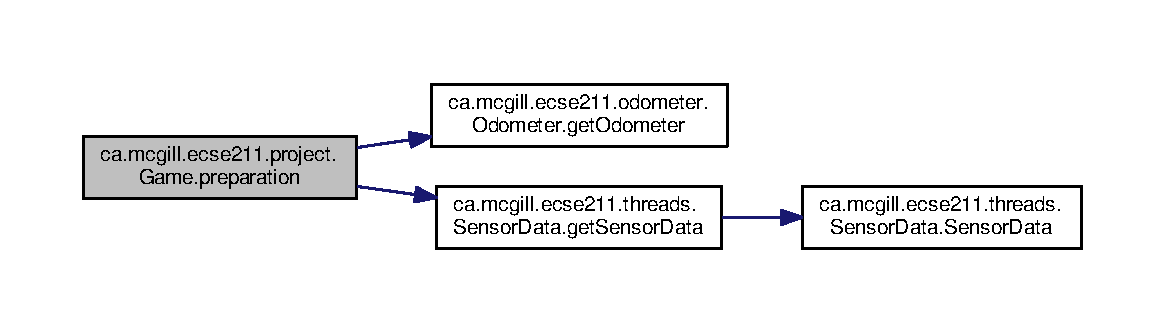
\includegraphics[width=350pt]{enumca_1_1mcgill_1_1ecse211_1_1project_1_1_game_a8f3c5b18f98ee56f5f03afd72fa40bcb_cgraph}
\end{center}
\end{figure}
\mbox{\Hypertarget{enumca_1_1mcgill_1_1ecse211_1_1project_1_1_game_a032b53e9b16b9d470b461de4a311a698}\label{enumca_1_1mcgill_1_1ecse211_1_1project_1_1_game_a032b53e9b16b9d470b461de4a311a698}} 
\index{ca\+::mcgill\+::ecse211\+::project\+::\+Game@{ca\+::mcgill\+::ecse211\+::project\+::\+Game}!read\+Data@{read\+Data}}
\index{read\+Data@{read\+Data}!ca\+::mcgill\+::ecse211\+::project\+::\+Game@{ca\+::mcgill\+::ecse211\+::project\+::\+Game}}
\subsubsection{\texorpdfstring{read\+Data()}{readData()}}
{\footnotesize\ttfamily void ca.\+mcgill.\+ecse211.\+project.\+Game.\+read\+Data (\begin{DoxyParamCaption}{ }\end{DoxyParamCaption})}

This method reads data from the \hyperlink{enumca_1_1mcgill_1_1ecse211_1_1project_1_1_wi_fi}{Wi\+Fi} class (using another thread) 

Definition at line 245 of file Game.\+java.


\begin{DoxyCode}
245                          \{
246     WiFi.readData();
247   \}
\end{DoxyCode}
Here is the call graph for this function\+:\nopagebreak
\begin{figure}[H]
\begin{center}
\leavevmode
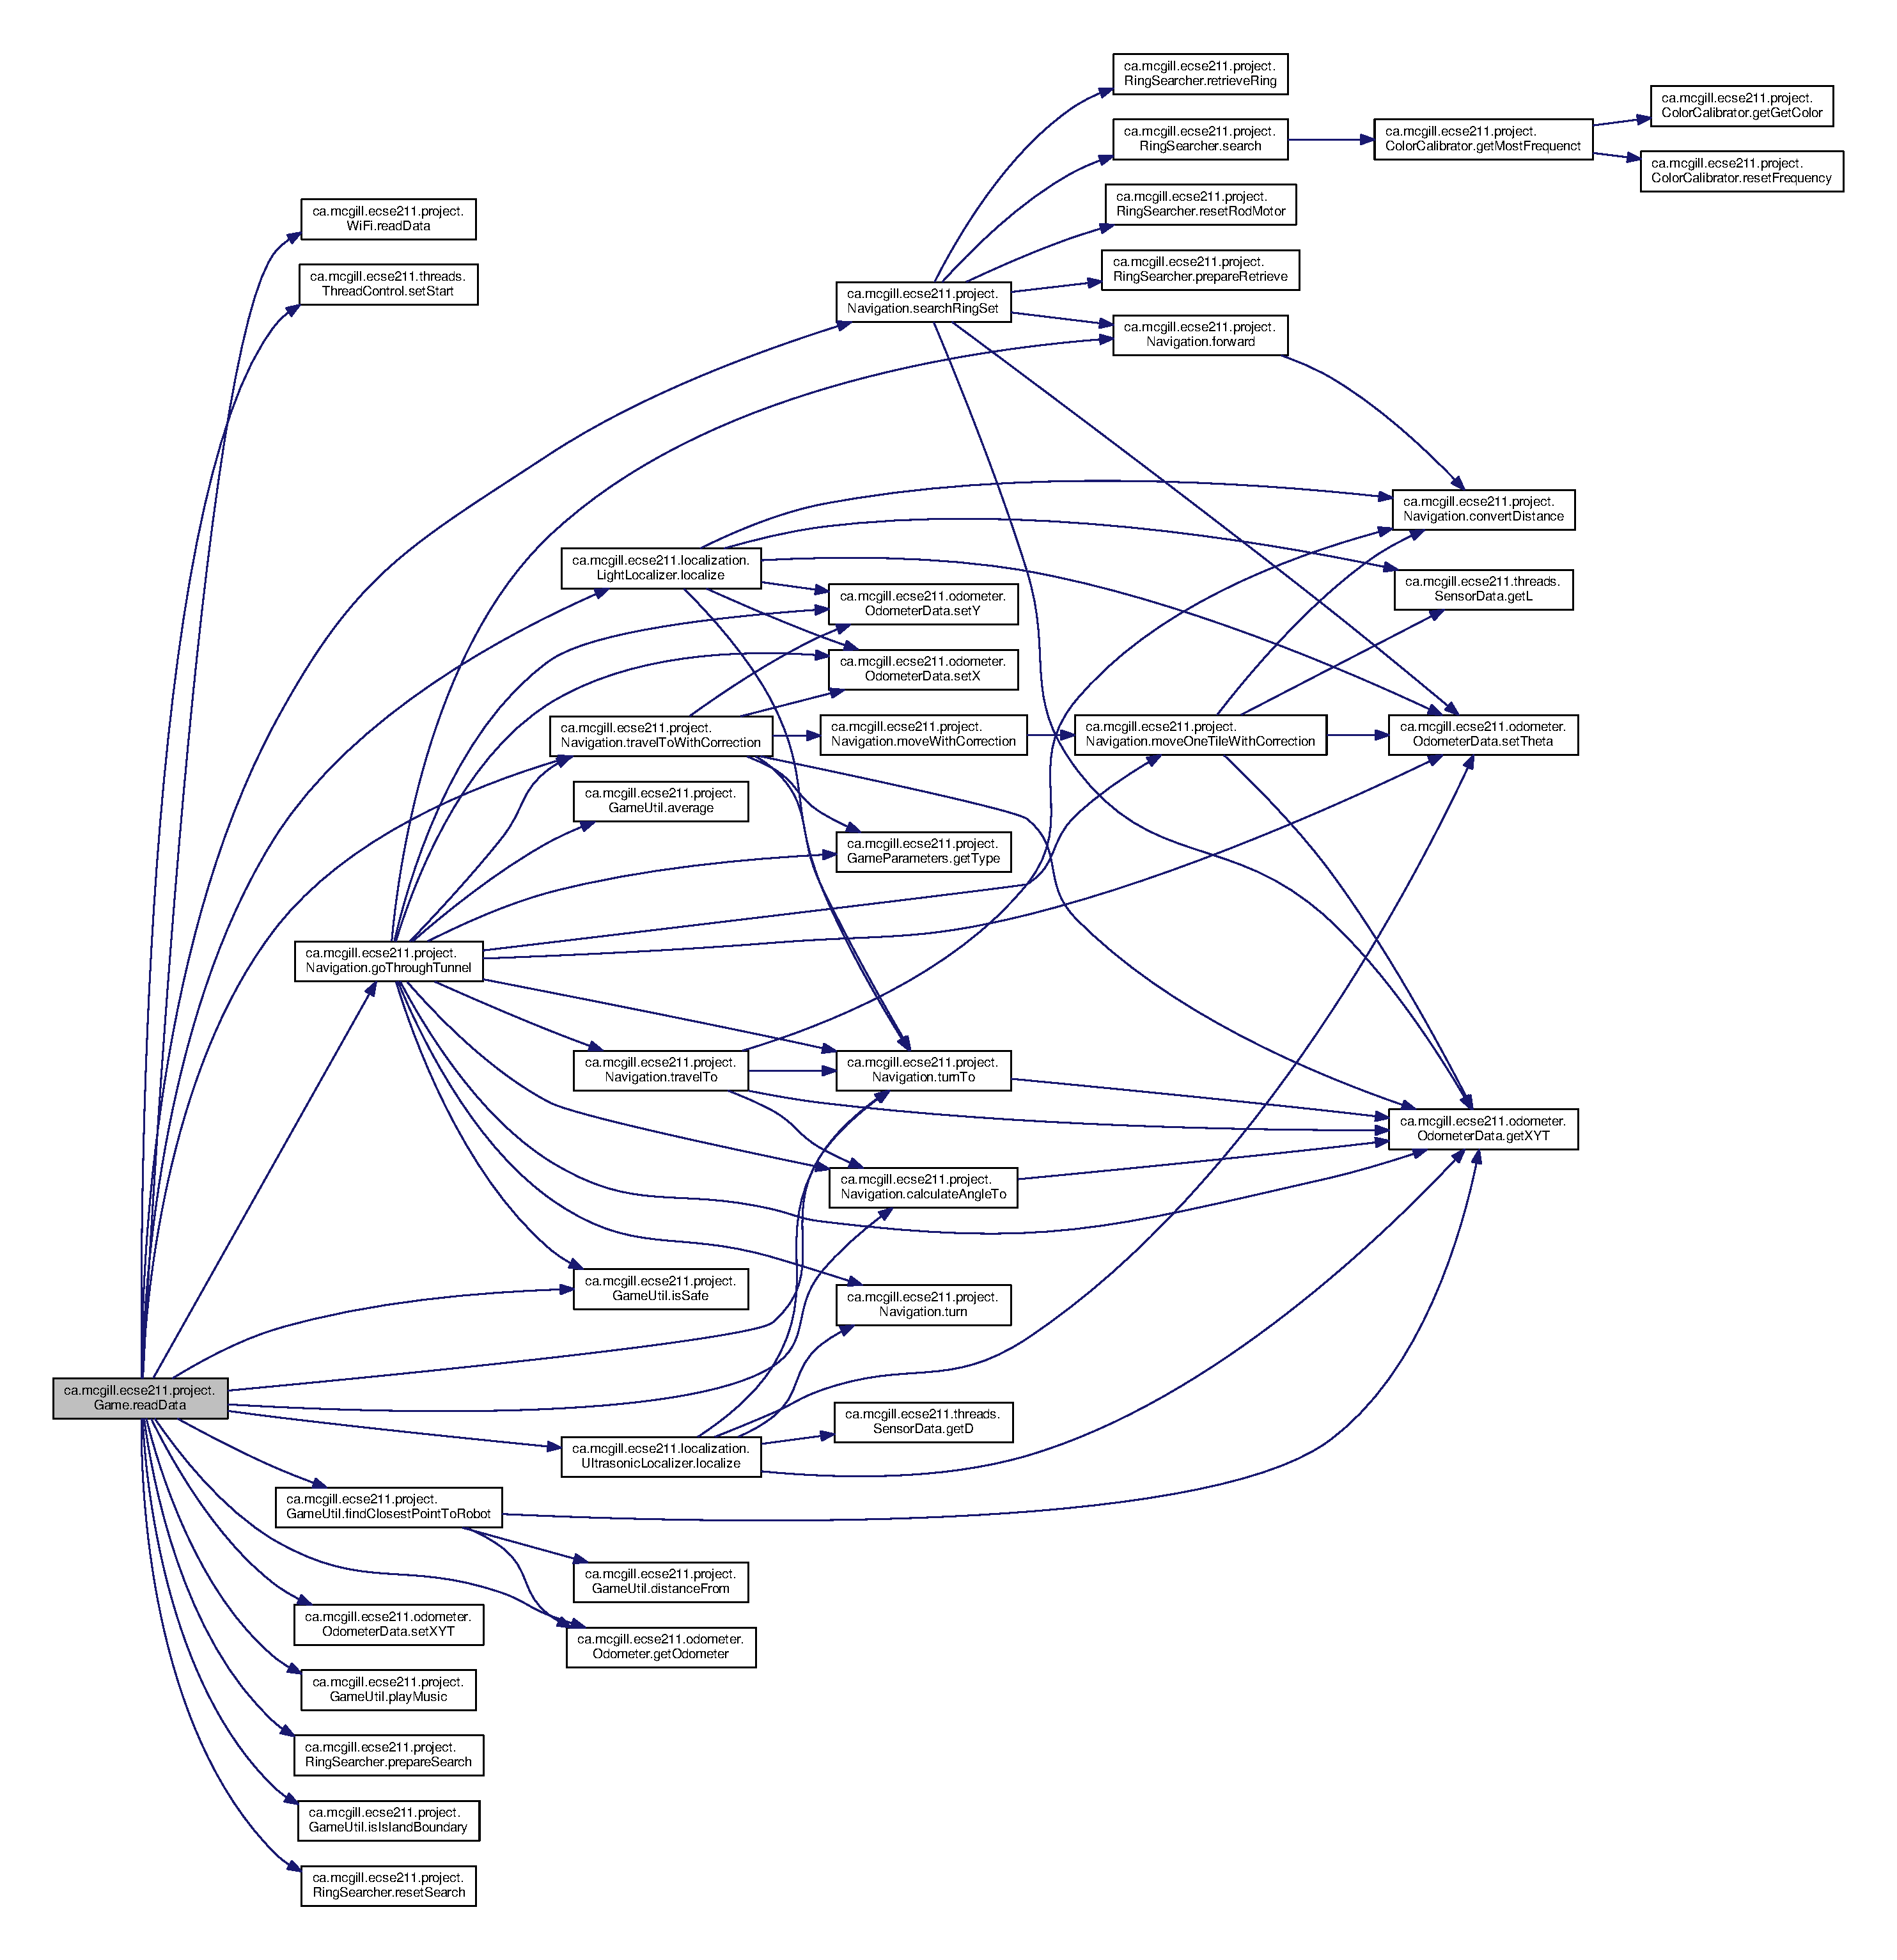
\includegraphics[width=350pt]{enumca_1_1mcgill_1_1ecse211_1_1project_1_1_game_a032b53e9b16b9d470b461de4a311a698_cgraph}
\end{center}
\end{figure}
\mbox{\Hypertarget{enumca_1_1mcgill_1_1ecse211_1_1project_1_1_game_a5b304a6a59ddee3f8c7d37bba8a4c129}\label{enumca_1_1mcgill_1_1ecse211_1_1project_1_1_game_a5b304a6a59ddee3f8c7d37bba8a4c129}} 
\index{ca\+::mcgill\+::ecse211\+::project\+::\+Game@{ca\+::mcgill\+::ecse211\+::project\+::\+Game}!ready@{ready}}
\index{ready@{ready}!ca\+::mcgill\+::ecse211\+::project\+::\+Game@{ca\+::mcgill\+::ecse211\+::project\+::\+Game}}
\subsubsection{\texorpdfstring{ready()}{ready()}}
{\footnotesize\ttfamily boolean ca.\+mcgill.\+ecse211.\+project.\+Game.\+ready (\begin{DoxyParamCaption}\item[{\hyperlink{classca_1_1mcgill_1_1ecse211_1_1localization_1_1_ultrasonic_localizer}{Ultrasonic\+Localizer}}]{us,  }\item[{\hyperlink{classca_1_1mcgill_1_1ecse211_1_1localization_1_1_light_localizer}{Light\+Localizer}}]{lg\+Loc }\end{DoxyParamCaption})}

This method performs localizes our robot

\begin{DoxyReturn}{Returns}
A boolean that denotes whether our state transition occurred 
\end{DoxyReturn}


Definition at line 71 of file Game.\+java.


\begin{DoxyCode}
71                                                                      \{
72     \textcolor{keywordtype}{boolean} wasEventProcessed = \textcolor{keyword}{false};
73 
74     Status aStatus = status;
75     \textcolor{keywordflow}{switch} (aStatus) \{
76       \textcolor{keywordflow}{case} Idle:
77         \textcolor{keywordflow}{try} \{
78           localizeAndReadData(us, lgLoc);
79         \} \textcolor{keywordflow}{catch} (OdometerExceptions e) \{
80           e.printStackTrace();
81         \}
82         setStatus(Status.Localized);
83         wasEventProcessed = \textcolor{keyword}{true};
84         \textcolor{keywordflow}{break};
85       \textcolor{keywordflow}{default}:
86         \textcolor{comment}{// Other states do respond to this event}
87         \textcolor{keywordflow}{break};
88     \}
89     Sound.beep();
90     Sound.beep();
91     \textcolor{keywordflow}{return} wasEventProcessed;
92   \}
\end{DoxyCode}
\mbox{\Hypertarget{enumca_1_1mcgill_1_1ecse211_1_1project_1_1_game_adf69abe44e952d627fb9e6a2f678cb5e}\label{enumca_1_1mcgill_1_1ecse211_1_1project_1_1_game_adf69abe44e952d627fb9e6a2f678cb5e}} 
\index{ca\+::mcgill\+::ecse211\+::project\+::\+Game@{ca\+::mcgill\+::ecse211\+::project\+::\+Game}!run\+Game@{run\+Game}}
\index{run\+Game@{run\+Game}!ca\+::mcgill\+::ecse211\+::project\+::\+Game@{ca\+::mcgill\+::ecse211\+::project\+::\+Game}}
\subsubsection{\texorpdfstring{run\+Game()}{runGame()}}
{\footnotesize\ttfamily void ca.\+mcgill.\+ecse211.\+project.\+Game.\+run\+Game (\begin{DoxyParamCaption}{ }\end{DoxyParamCaption}) throws \hyperlink{classca_1_1mcgill_1_1ecse211_1_1odometer_1_1_odometer_exceptions}{Odometer\+Exceptions}}

This method is called when the after the robot has been prepared and is ready to compete


\begin{DoxyExceptions}{Exceptions}
{\em Odometer\+Exceptions} & \\
\hline
\end{DoxyExceptions}


Definition at line 421 of file Game.\+java.


\begin{DoxyCode}
421                                                   \{
422     GameParameters.Demo = DemoType.Beta;
423     \textcolor{comment}{// Start localizing}
424     \textcolor{keyword}{final} Navigation navigation = \textcolor{keyword}{new} Navigation(\hyperlink{enumca_1_1mcgill_1_1ecse211_1_1project_1_1_game_a7c673571bf50fdb6917a9d7bb671e003}{leftMotor}, \hyperlink{enumca_1_1mcgill_1_1ecse211_1_1project_1_1_game_a7a05fcf37c4435c32270776a427ba0d2}{rightMotor});
425     \textcolor{keyword}{final} UltrasonicLocalizer usLoc = \textcolor{keyword}{new} UltrasonicLocalizer(navigation, 
      \hyperlink{enumca_1_1mcgill_1_1ecse211_1_1project_1_1_game_a7c673571bf50fdb6917a9d7bb671e003}{leftMotor}, \hyperlink{enumca_1_1mcgill_1_1ecse211_1_1project_1_1_game_a7a05fcf37c4435c32270776a427ba0d2}{rightMotor});
426     \textcolor{keyword}{final} LightLocalizer lgLoc = \textcolor{keyword}{new} LightLocalizer(navigation, \hyperlink{enumca_1_1mcgill_1_1ecse211_1_1project_1_1_game_a7c673571bf50fdb6917a9d7bb671e003}{leftMotor}, 
      \hyperlink{enumca_1_1mcgill_1_1ecse211_1_1project_1_1_game_a7a05fcf37c4435c32270776a427ba0d2}{rightMotor});
427     \textcolor{keyword}{final} RingSearcher searcher = \textcolor{keyword}{new} RingSearcher(\hyperlink{enumca_1_1mcgill_1_1ecse211_1_1project_1_1_game_aa94b85dc88de85d959677bd6c0f98989}{sensorMotor}, 
      \hyperlink{enumca_1_1mcgill_1_1ecse211_1_1project_1_1_game_abc070af2fa5a5cda6d81977b35aacfb4}{rodMotor});
428 
429     Button.waitForAnyPress(); \textcolor{comment}{// Wait for button press to start}
430     \hyperlink{enumca_1_1mcgill_1_1ecse211_1_1project_1_1_game_a6584b6534b14ba43dc1444084a925a20}{INSTANCE}.ready(usLoc, lgLoc);
431 
432     \textcolor{comment}{// instantiate path finder}
433     GameUtil.searchingFinder =
434         \textcolor{keyword}{new} GameUtil.PathFinder(GameParameters.Island\_LL, GameParameters.Island\_UR);
435     GameUtil.startingFinder = \textcolor{keyword}{new} GameUtil.PathFinder(GameParameters.US\_LL, GameParameters.US\_UR);
436     \hyperlink{enumca_1_1mcgill_1_1ecse211_1_1project_1_1_game_a6584b6534b14ba43dc1444084a925a20}{INSTANCE}.navigateToTunnel(navigation, searcher);
437     \hyperlink{enumca_1_1mcgill_1_1ecse211_1_1project_1_1_game_a6584b6534b14ba43dc1444084a925a20}{INSTANCE}.navigateToAndSearcherTree(navigation, searcher);
438     \hyperlink{enumca_1_1mcgill_1_1ecse211_1_1project_1_1_game_a6584b6534b14ba43dc1444084a925a20}{INSTANCE}.navigateToTunnel(navigation, searcher);
439     \hyperlink{enumca_1_1mcgill_1_1ecse211_1_1project_1_1_game_a6584b6534b14ba43dc1444084a925a20}{INSTANCE}.navigateToStart(navigation, searcher);
440   \}
\end{DoxyCode}


\subsection{Member Data Documentation}
\mbox{\Hypertarget{enumca_1_1mcgill_1_1ecse211_1_1project_1_1_game_a7c673571bf50fdb6917a9d7bb671e003}\label{enumca_1_1mcgill_1_1ecse211_1_1project_1_1_game_a7c673571bf50fdb6917a9d7bb671e003}} 
\index{ca\+::mcgill\+::ecse211\+::project\+::\+Game@{ca\+::mcgill\+::ecse211\+::project\+::\+Game}!left\+Motor@{left\+Motor}}
\index{left\+Motor@{left\+Motor}!ca\+::mcgill\+::ecse211\+::project\+::\+Game@{ca\+::mcgill\+::ecse211\+::project\+::\+Game}}
\subsubsection{\texorpdfstring{left\+Motor}{leftMotor}}
{\footnotesize\ttfamily  static  final E\+V3\+Large\+Regulated\+Motor ca.\+mcgill.\+ecse211.\+project.\+Game.\+left\+Motor\hspace{0.3cm}{\ttfamily [static]}}

{\bfseries Initial value\+:}
\begin{DoxyCode}
=
      \textcolor{keyword}{new} EV3LargeRegulatedMotor(LocalEV3.get().getPort(\textcolor{stringliteral}{"A"}))
\end{DoxyCode}
This variable stores an E\+V3\+Large\+Regulated\+Motor object instance that allows control of the left motor connected to port A 

Definition at line 197 of file Game.\+java.

\mbox{\Hypertarget{enumca_1_1mcgill_1_1ecse211_1_1project_1_1_game_af24a953a0c3438670220dde36c532b5d}\label{enumca_1_1mcgill_1_1ecse211_1_1project_1_1_game_af24a953a0c3438670220dde36c532b5d}} 
\index{ca\+::mcgill\+::ecse211\+::project\+::\+Game@{ca\+::mcgill\+::ecse211\+::project\+::\+Game}!rgb\+Poller@{rgb\+Poller}}
\index{rgb\+Poller@{rgb\+Poller}!ca\+::mcgill\+::ecse211\+::project\+::\+Game@{ca\+::mcgill\+::ecse211\+::project\+::\+Game}}
\subsubsection{\texorpdfstring{rgb\+Poller}{rgbPoller}}
{\footnotesize\ttfamily \hyperlink{classca_1_1mcgill_1_1ecse211_1_1threads_1_1_thread_control}{Thread\+Control} ca.\+mcgill.\+ecse211.\+project.\+Game.\+rgb\+Poller}

This variable stores a Thread\+Controller instance that controls our R\+GB sensor 

Definition at line 181 of file Game.\+java.

\mbox{\Hypertarget{enumca_1_1mcgill_1_1ecse211_1_1project_1_1_game_a7a05fcf37c4435c32270776a427ba0d2}\label{enumca_1_1mcgill_1_1ecse211_1_1project_1_1_game_a7a05fcf37c4435c32270776a427ba0d2}} 
\index{ca\+::mcgill\+::ecse211\+::project\+::\+Game@{ca\+::mcgill\+::ecse211\+::project\+::\+Game}!right\+Motor@{right\+Motor}}
\index{right\+Motor@{right\+Motor}!ca\+::mcgill\+::ecse211\+::project\+::\+Game@{ca\+::mcgill\+::ecse211\+::project\+::\+Game}}
\subsubsection{\texorpdfstring{right\+Motor}{rightMotor}}
{\footnotesize\ttfamily  static  final E\+V3\+Large\+Regulated\+Motor ca.\+mcgill.\+ecse211.\+project.\+Game.\+right\+Motor\hspace{0.3cm}{\ttfamily [static]}}

{\bfseries Initial value\+:}
\begin{DoxyCode}
=
      \textcolor{keyword}{new} EV3LargeRegulatedMotor(LocalEV3.get().getPort(\textcolor{stringliteral}{"D"}))
\end{DoxyCode}
This variable stores an E\+V3\+Large\+Regulated\+Motor object instance that allows control of the right motor connected to port D 

Definition at line 204 of file Game.\+java.

\mbox{\Hypertarget{enumca_1_1mcgill_1_1ecse211_1_1project_1_1_game_abc070af2fa5a5cda6d81977b35aacfb4}\label{enumca_1_1mcgill_1_1ecse211_1_1project_1_1_game_abc070af2fa5a5cda6d81977b35aacfb4}} 
\index{ca\+::mcgill\+::ecse211\+::project\+::\+Game@{ca\+::mcgill\+::ecse211\+::project\+::\+Game}!rod\+Motor@{rod\+Motor}}
\index{rod\+Motor@{rod\+Motor}!ca\+::mcgill\+::ecse211\+::project\+::\+Game@{ca\+::mcgill\+::ecse211\+::project\+::\+Game}}
\subsubsection{\texorpdfstring{rod\+Motor}{rodMotor}}
{\footnotesize\ttfamily  static  final E\+V3\+Large\+Regulated\+Motor ca.\+mcgill.\+ecse211.\+project.\+Game.\+rod\+Motor\hspace{0.3cm}{\ttfamily [static]}}

{\bfseries Initial value\+:}
\begin{DoxyCode}
=
      \textcolor{keyword}{new} EV3LargeRegulatedMotor(LocalEV3.get().getPort(\textcolor{stringliteral}{"B"}))
\end{DoxyCode}
This variable stores an E\+V3\+Large\+Regulated\+Motor object instance that allows control of the motor on the rod for collecting rings 

Definition at line 218 of file Game.\+java.

\mbox{\Hypertarget{enumca_1_1mcgill_1_1ecse211_1_1project_1_1_game_ab940d1a52b9759294dc0229e0fd6bc06}\label{enumca_1_1mcgill_1_1ecse211_1_1project_1_1_game_ab940d1a52b9759294dc0229e0fd6bc06}} 
\index{ca\+::mcgill\+::ecse211\+::project\+::\+Game@{ca\+::mcgill\+::ecse211\+::project\+::\+Game}!S\+E\+N\+\_\+\+D\+IS@{S\+E\+N\+\_\+\+D\+IS}}
\index{S\+E\+N\+\_\+\+D\+IS@{S\+E\+N\+\_\+\+D\+IS}!ca\+::mcgill\+::ecse211\+::project\+::\+Game@{ca\+::mcgill\+::ecse211\+::project\+::\+Game}}
\subsubsection{\texorpdfstring{S\+E\+N\+\_\+\+D\+IS}{SEN\_DIS}}
{\footnotesize\ttfamily  static  final double ca.\+mcgill.\+ecse211.\+project.\+Game.\+S\+E\+N\+\_\+\+D\+IS = 4.\+2\hspace{0.3cm}{\ttfamily [static]}}

This variable stores the distance between the light sensor and center of the robot in cm 

Definition at line 240 of file Game.\+java.

\mbox{\Hypertarget{enumca_1_1mcgill_1_1ecse211_1_1project_1_1_game_aa94b85dc88de85d959677bd6c0f98989}\label{enumca_1_1mcgill_1_1ecse211_1_1project_1_1_game_aa94b85dc88de85d959677bd6c0f98989}} 
\index{ca\+::mcgill\+::ecse211\+::project\+::\+Game@{ca\+::mcgill\+::ecse211\+::project\+::\+Game}!sensor\+Motor@{sensor\+Motor}}
\index{sensor\+Motor@{sensor\+Motor}!ca\+::mcgill\+::ecse211\+::project\+::\+Game@{ca\+::mcgill\+::ecse211\+::project\+::\+Game}}
\subsubsection{\texorpdfstring{sensor\+Motor}{sensorMotor}}
{\footnotesize\ttfamily  static  final E\+V3\+Large\+Regulated\+Motor ca.\+mcgill.\+ecse211.\+project.\+Game.\+sensor\+Motor\hspace{0.3cm}{\ttfamily [static]}}

{\bfseries Initial value\+:}
\begin{DoxyCode}
=
      \textcolor{keyword}{new} EV3LargeRegulatedMotor(LocalEV3.get().getPort(\textcolor{stringliteral}{"C"}))
\end{DoxyCode}
This variable stores an E\+V3\+Large\+Regulated\+Motor object instance that allows control of the motor on storage rod 

Definition at line 211 of file Game.\+java.

\mbox{\Hypertarget{enumca_1_1mcgill_1_1ecse211_1_1project_1_1_game_a72c2224ad4dd557dde445ebc4baaf531}\label{enumca_1_1mcgill_1_1ecse211_1_1project_1_1_game_a72c2224ad4dd557dde445ebc4baaf531}} 
\index{ca\+::mcgill\+::ecse211\+::project\+::\+Game@{ca\+::mcgill\+::ecse211\+::project\+::\+Game}!T\+I\+LE@{T\+I\+LE}}
\index{T\+I\+LE@{T\+I\+LE}!ca\+::mcgill\+::ecse211\+::project\+::\+Game@{ca\+::mcgill\+::ecse211\+::project\+::\+Game}}
\subsubsection{\texorpdfstring{T\+I\+LE}{TILE}}
{\footnotesize\ttfamily  static  final double ca.\+mcgill.\+ecse211.\+project.\+Game.\+T\+I\+LE = 30.\+48\hspace{0.3cm}{\ttfamily [static]}}

This variable stores the length of a tile in cm 

Definition at line 224 of file Game.\+java.

\mbox{\Hypertarget{enumca_1_1mcgill_1_1ecse211_1_1project_1_1_game_a64cf12cdd6772ac1ce351ff1dfadd626}\label{enumca_1_1mcgill_1_1ecse211_1_1project_1_1_game_a64cf12cdd6772ac1ce351ff1dfadd626}} 
\index{ca\+::mcgill\+::ecse211\+::project\+::\+Game@{ca\+::mcgill\+::ecse211\+::project\+::\+Game}!T\+R\+A\+CK@{T\+R\+A\+CK}}
\index{T\+R\+A\+CK@{T\+R\+A\+CK}!ca\+::mcgill\+::ecse211\+::project\+::\+Game@{ca\+::mcgill\+::ecse211\+::project\+::\+Game}}
\subsubsection{\texorpdfstring{T\+R\+A\+CK}{TRACK}}
{\footnotesize\ttfamily  static  final double ca.\+mcgill.\+ecse211.\+project.\+Game.\+T\+R\+A\+CK = 11.\+5\hspace{0.3cm}{\ttfamily [static]}}

This variable holds the track distance between the center of the wheels in cm (measured and adjusted based on trial and error) 

Definition at line 235 of file Game.\+java.

\mbox{\Hypertarget{enumca_1_1mcgill_1_1ecse211_1_1project_1_1_game_af6fee74efff891793b32352caa110465}\label{enumca_1_1mcgill_1_1ecse211_1_1project_1_1_game_af6fee74efff891793b32352caa110465}} 
\index{ca\+::mcgill\+::ecse211\+::project\+::\+Game@{ca\+::mcgill\+::ecse211\+::project\+::\+Game}!us\+Poller@{us\+Poller}}
\index{us\+Poller@{us\+Poller}!ca\+::mcgill\+::ecse211\+::project\+::\+Game@{ca\+::mcgill\+::ecse211\+::project\+::\+Game}}
\subsubsection{\texorpdfstring{us\+Poller}{usPoller}}
{\footnotesize\ttfamily \hyperlink{classca_1_1mcgill_1_1ecse211_1_1threads_1_1_thread_control}{Thread\+Control} ca.\+mcgill.\+ecse211.\+project.\+Game.\+us\+Poller}

This variable stores a Thread\+Controller instance that controls our ultrasonic sensor 

Definition at line 191 of file Game.\+java.

\mbox{\Hypertarget{enumca_1_1mcgill_1_1ecse211_1_1project_1_1_game_a91bd64670c2a91d006c907142783b1f8}\label{enumca_1_1mcgill_1_1ecse211_1_1project_1_1_game_a91bd64670c2a91d006c907142783b1f8}} 
\index{ca\+::mcgill\+::ecse211\+::project\+::\+Game@{ca\+::mcgill\+::ecse211\+::project\+::\+Game}!W\+H\+E\+E\+L\+\_\+\+R\+AD@{W\+H\+E\+E\+L\+\_\+\+R\+AD}}
\index{W\+H\+E\+E\+L\+\_\+\+R\+AD@{W\+H\+E\+E\+L\+\_\+\+R\+AD}!ca\+::mcgill\+::ecse211\+::project\+::\+Game@{ca\+::mcgill\+::ecse211\+::project\+::\+Game}}
\subsubsection{\texorpdfstring{W\+H\+E\+E\+L\+\_\+\+R\+AD}{WHEEL\_RAD}}
{\footnotesize\ttfamily  static  final double ca.\+mcgill.\+ecse211.\+project.\+Game.\+W\+H\+E\+E\+L\+\_\+\+R\+AD = 2.\+15\hspace{0.3cm}{\ttfamily [static]}}

This variable stores the radius of our wheels in cm 

Definition at line 229 of file Game.\+java.



The documentation for this enum was generated from the following file\+:\begin{DoxyCompactItemize}
\item 
/home/ccc/\+Final\+Project/src/ca/mcgill/ecse211/project/\hyperlink{_game_8java}{Game.\+java}\end{DoxyCompactItemize}

\hypertarget{classca_1_1mcgill_1_1ecse211_1_1project_1_1_game_parameters}{}\section{ca.\+mcgill.\+ecse211.\+project.\+Game\+Parameters Class Reference}
\label{classca_1_1mcgill_1_1ecse211_1_1project_1_1_game_parameters}\index{ca.\+mcgill.\+ecse211.\+project.\+Game\+Parameters@{ca.\+mcgill.\+ecse211.\+project.\+Game\+Parameters}}
\subsection*{Classes}
\begin{DoxyCompactItemize}
\item 
enum \hyperlink{enumca_1_1mcgill_1_1ecse211_1_1project_1_1_game_parameters_1_1_area_type}{Area\+Type}
\end{DoxyCompactItemize}
\subsection*{Static Public Member Functions}
\begin{DoxyCompactItemize}
\item 
static \hyperlink{enumca_1_1mcgill_1_1ecse211_1_1project_1_1_game_parameters_1_1_area_type}{Area\+Type} \hyperlink{classca_1_1mcgill_1_1ecse211_1_1project_1_1_game_parameters_afa2d71de18f6276782a702d7b74066e3}{get\+Type} (double x, double y)
\end{DoxyCompactItemize}
\subsection*{Static Public Attributes}
\begin{DoxyCompactItemize}
\item 
static int \mbox{[}$\,$\mbox{]} \hyperlink{classca_1_1mcgill_1_1ecse211_1_1project_1_1_game_parameters_aae8c69151bc01acce692b9119323bb46}{SC} = \{-\/1, -\/1\}
\item 
static int \mbox{[}$\,$\mbox{]} \hyperlink{classca_1_1mcgill_1_1ecse211_1_1project_1_1_game_parameters_aec739d9ebcbd75db6a77ec288ff974cf}{Grid\+\_\+\+LL} = \{0, 0\}
\item 
static int \mbox{[}$\,$\mbox{]} \hyperlink{classca_1_1mcgill_1_1ecse211_1_1project_1_1_game_parameters_ab79c9c891076d29cbe5ac053f617c381}{Grid\+\_\+\+UR} = \{15, 9\}
\item 
static int \hyperlink{classca_1_1mcgill_1_1ecse211_1_1project_1_1_game_parameters_a5a299e93e098c89d12be1072947d3bcb}{TR} = -\/1
\item 
static int \hyperlink{classca_1_1mcgill_1_1ecse211_1_1project_1_1_game_parameters_a15bc3c24f73d1ad29b6fe7fd9e1ef0e6}{Player\+Team\+Number} = -\/1
\item 
static int \hyperlink{classca_1_1mcgill_1_1ecse211_1_1project_1_1_game_parameters_a51c899921677197f960f39e6ed42c780}{Red\+Team} = -\/1
\item 
static int \hyperlink{classca_1_1mcgill_1_1ecse211_1_1project_1_1_game_parameters_aca550f5067892ceeb8f44ede61bbc90e}{Green\+Team} = -\/1
\item 
static int \hyperlink{classca_1_1mcgill_1_1ecse211_1_1project_1_1_game_parameters_acf0dce5eb9dc754248f0c3de997d2809}{Red\+Corner} = -\/1
\item 
static int \hyperlink{classca_1_1mcgill_1_1ecse211_1_1project_1_1_game_parameters_a7fe7f10f96800fbd5f2331e3aa608b66}{Green\+Corner} = -\/1
\item 
static int \mbox{[}$\,$\mbox{]} \hyperlink{classca_1_1mcgill_1_1ecse211_1_1project_1_1_game_parameters_ae3eb3c87467d3a7760cd619a96379a9e}{Red\+\_\+\+LL} = \{0, 5\}
\item 
static int \mbox{[}$\,$\mbox{]} \hyperlink{classca_1_1mcgill_1_1ecse211_1_1project_1_1_game_parameters_a81ddd789119962c32fe6d7f9cce4f240}{Red\+\_\+\+UR} = \{4, 9\}
\item 
static int \mbox{[}$\,$\mbox{]} \hyperlink{classca_1_1mcgill_1_1ecse211_1_1project_1_1_game_parameters_a24e38b735e194403bf2b9877241969c1}{Green\+\_\+\+LL} = \{10, 0\}
\item 
static int \mbox{[}$\,$\mbox{]} \hyperlink{classca_1_1mcgill_1_1ecse211_1_1project_1_1_game_parameters_aedb13ca3822f3581bdffd464891b1494}{Green\+\_\+\+UR} = \{15, 4\}
\item 
static int \mbox{[}$\,$\mbox{]} \hyperlink{classca_1_1mcgill_1_1ecse211_1_1project_1_1_game_parameters_a8695da7f04954ea1513082740fd2d57f}{B\+R\+R\+\_\+\+LL} = \{4, 7\}
\item 
static int \mbox{[}$\,$\mbox{]} \hyperlink{classca_1_1mcgill_1_1ecse211_1_1project_1_1_game_parameters_a720d0ae20fc2466e7b77fda14bf374f3}{B\+R\+R\+\_\+\+UR} = \{6, 8\}
\item 
static int \mbox{[}$\,$\mbox{]} \hyperlink{classca_1_1mcgill_1_1ecse211_1_1project_1_1_game_parameters_ae6824f16adf03173062767f99d46b6e0}{B\+R\+G\+\_\+\+LL} = \{10, 3\}
\item 
static int \mbox{[}$\,$\mbox{]} \hyperlink{classca_1_1mcgill_1_1ecse211_1_1project_1_1_game_parameters_a644c339e7b0f11c5780f9c7de34e1e07}{B\+R\+G\+\_\+\+UR} = \{11, 5\}
\item 
static int \mbox{[}$\,$\mbox{]} \hyperlink{classca_1_1mcgill_1_1ecse211_1_1project_1_1_game_parameters_ac642730053a35524ce70866289ca10b9}{T\+R\+\_\+\+LL} = \{7, 6\}
\item 
static int \mbox{[}$\,$\mbox{]} \hyperlink{classca_1_1mcgill_1_1ecse211_1_1project_1_1_game_parameters_a45c465e9f0b53a4e752a398036be13f5}{T\+R\+\_\+\+UR} = \{8, 7\}
\item 
static int \mbox{[}$\,$\mbox{]} \hyperlink{classca_1_1mcgill_1_1ecse211_1_1project_1_1_game_parameters_a0fefeecefd65deabea205bd9d628bf76}{T\+G\+\_\+\+LL} = \{13, 7\}
\item 
static int \mbox{[}$\,$\mbox{]} \hyperlink{classca_1_1mcgill_1_1ecse211_1_1project_1_1_game_parameters_aa8220987d04f322d9480db7cc073ffd2}{T\+G\+\_\+\+UR} = \{14, 8\}
\end{DoxyCompactItemize}


\subsection{Detailed Description}
This class contains all the game parameters needed for the competition

\begin{DoxyAuthor}{Author}
Caspar Cedro 

Percy Chen 

Patrick Erath 

Anssam Ghezala 

Susan Matuszewski 

Kamy Moussavi Kafi 
\end{DoxyAuthor}


Definition at line 13 of file Game\+Parameters.\+java.



\subsection{Member Function Documentation}
\mbox{\Hypertarget{classca_1_1mcgill_1_1ecse211_1_1project_1_1_game_parameters_afa2d71de18f6276782a702d7b74066e3}\label{classca_1_1mcgill_1_1ecse211_1_1project_1_1_game_parameters_afa2d71de18f6276782a702d7b74066e3}} 
\index{ca\+::mcgill\+::ecse211\+::project\+::\+Game\+Parameters@{ca\+::mcgill\+::ecse211\+::project\+::\+Game\+Parameters}!get\+Type@{get\+Type}}
\index{get\+Type@{get\+Type}!ca\+::mcgill\+::ecse211\+::project\+::\+Game\+Parameters@{ca\+::mcgill\+::ecse211\+::project\+::\+Game\+Parameters}}
\subsubsection{\texorpdfstring{get\+Type()}{getType()}}
{\footnotesize\ttfamily static \hyperlink{enumca_1_1mcgill_1_1ecse211_1_1project_1_1_game_parameters_1_1_area_type}{Area\+Type} ca.\+mcgill.\+ecse211.\+project.\+Game\+Parameters.\+get\+Type (\begin{DoxyParamCaption}\item[{double}]{x,  }\item[{double}]{y }\end{DoxyParamCaption})\hspace{0.3cm}{\ttfamily [static]}}

Giving a coordinate, find the type of area it belongs to 
\begin{DoxyParams}{Parameters}
{\em x} & x coordinate \\
\hline
{\em y} & y coordinate \\
\hline
\end{DoxyParams}
\begin{DoxyReturn}{Returns}
\+: the type of area the point belongs to 
\end{DoxyReturn}


Definition at line 200 of file Game\+Parameters.\+java.


\begin{DoxyCode}
200                                                      \{
201     \textcolor{keywordflow}{return} AreaType.Searching;
202   \}
\end{DoxyCode}


\subsection{Member Data Documentation}
\mbox{\Hypertarget{classca_1_1mcgill_1_1ecse211_1_1project_1_1_game_parameters_ae6824f16adf03173062767f99d46b6e0}\label{classca_1_1mcgill_1_1ecse211_1_1project_1_1_game_parameters_ae6824f16adf03173062767f99d46b6e0}} 
\index{ca\+::mcgill\+::ecse211\+::project\+::\+Game\+Parameters@{ca\+::mcgill\+::ecse211\+::project\+::\+Game\+Parameters}!B\+R\+G\+\_\+\+LL@{B\+R\+G\+\_\+\+LL}}
\index{B\+R\+G\+\_\+\+LL@{B\+R\+G\+\_\+\+LL}!ca\+::mcgill\+::ecse211\+::project\+::\+Game\+Parameters@{ca\+::mcgill\+::ecse211\+::project\+::\+Game\+Parameters}}
\subsubsection{\texorpdfstring{B\+R\+G\+\_\+\+LL}{BRG\_LL}}
{\footnotesize\ttfamily int \mbox{[}$\,$\mbox{]} ca.\+mcgill.\+ecse211.\+project.\+Game\+Parameters.\+B\+R\+G\+\_\+\+LL = \{10, 3\}\hspace{0.3cm}{\ttfamily [static]}}

This variable stores the lower left hand corner of the green tunnel footprint. \mbox{[}0\mbox{]} = x coordinate, \mbox{[}1\mbox{]} = y coordinate min B\+R\+G\+\_\+\+UR\mbox{[}0\mbox{]} -\/ B\+R\+G\+\_\+\+LL\mbox{[}0\mbox{]} = 1 max B\+R\+G\+\_\+\+UR\mbox{[}0\mbox{]} -\/ B\+R\+G\+\_\+\+LL\mbox{[}0\mbox{]} = 2 min B\+R\+G\+\_\+\+UR\mbox{[}1\mbox{]} -\/ B\+R\+G\+\_\+\+LL\mbox{[}1\mbox{]} = 1 max B\+R\+G\+\_\+\+UR\mbox{[}1\mbox{]} -\/ B\+R\+G\+\_\+\+LL\mbox{[}1\mbox{]} = 2 

Definition at line 142 of file Game\+Parameters.\+java.

\mbox{\Hypertarget{classca_1_1mcgill_1_1ecse211_1_1project_1_1_game_parameters_a644c339e7b0f11c5780f9c7de34e1e07}\label{classca_1_1mcgill_1_1ecse211_1_1project_1_1_game_parameters_a644c339e7b0f11c5780f9c7de34e1e07}} 
\index{ca\+::mcgill\+::ecse211\+::project\+::\+Game\+Parameters@{ca\+::mcgill\+::ecse211\+::project\+::\+Game\+Parameters}!B\+R\+G\+\_\+\+UR@{B\+R\+G\+\_\+\+UR}}
\index{B\+R\+G\+\_\+\+UR@{B\+R\+G\+\_\+\+UR}!ca\+::mcgill\+::ecse211\+::project\+::\+Game\+Parameters@{ca\+::mcgill\+::ecse211\+::project\+::\+Game\+Parameters}}
\subsubsection{\texorpdfstring{B\+R\+G\+\_\+\+UR}{BRG\_UR}}
{\footnotesize\ttfamily int \mbox{[}$\,$\mbox{]} ca.\+mcgill.\+ecse211.\+project.\+Game\+Parameters.\+B\+R\+G\+\_\+\+UR = \{11, 5\}\hspace{0.3cm}{\ttfamily [static]}}

This variable stores the upper right hand corner of the green tunnel footprint. \mbox{[}0\mbox{]} = x coordinate, \mbox{[}1\mbox{]} = y coordinate min B\+R\+G\+\_\+\+UR\mbox{[}0\mbox{]} -\/ B\+R\+G\+\_\+\+LL\mbox{[}0\mbox{]} = 1 max B\+R\+G\+\_\+\+UR\mbox{[}0\mbox{]} -\/ B\+R\+G\+\_\+\+LL\mbox{[}0\mbox{]} = 2 min B\+R\+G\+\_\+\+UR\mbox{[}1\mbox{]} -\/ B\+R\+G\+\_\+\+LL\mbox{[}1\mbox{]} = 1 max B\+R\+G\+\_\+\+UR\mbox{[}1\mbox{]} -\/ B\+R\+G\+\_\+\+LL\mbox{[}1\mbox{]} = 2 

Definition at line 152 of file Game\+Parameters.\+java.

\mbox{\Hypertarget{classca_1_1mcgill_1_1ecse211_1_1project_1_1_game_parameters_a8695da7f04954ea1513082740fd2d57f}\label{classca_1_1mcgill_1_1ecse211_1_1project_1_1_game_parameters_a8695da7f04954ea1513082740fd2d57f}} 
\index{ca\+::mcgill\+::ecse211\+::project\+::\+Game\+Parameters@{ca\+::mcgill\+::ecse211\+::project\+::\+Game\+Parameters}!B\+R\+R\+\_\+\+LL@{B\+R\+R\+\_\+\+LL}}
\index{B\+R\+R\+\_\+\+LL@{B\+R\+R\+\_\+\+LL}!ca\+::mcgill\+::ecse211\+::project\+::\+Game\+Parameters@{ca\+::mcgill\+::ecse211\+::project\+::\+Game\+Parameters}}
\subsubsection{\texorpdfstring{B\+R\+R\+\_\+\+LL}{BRR\_LL}}
{\footnotesize\ttfamily int \mbox{[}$\,$\mbox{]} ca.\+mcgill.\+ecse211.\+project.\+Game\+Parameters.\+B\+R\+R\+\_\+\+LL = \{4, 7\}\hspace{0.3cm}{\ttfamily [static]}}

This variable stores the lower left hand corner of the red tunnel footprint. \mbox{[}0\mbox{]} = x coordinate, \mbox{[}1\mbox{]} = y coordinate min B\+R\+R\+\_\+\+UR\mbox{[}0\mbox{]} -\/ B\+R\+R\+\_\+\+LL\mbox{[}0\mbox{]} = 1 max B\+R\+R\+\_\+\+UR\mbox{[}0\mbox{]} -\/ B\+R\+R\+\_\+\+LL\mbox{[}0\mbox{]} = 2 min B\+R\+R\+\_\+\+UR\mbox{[}1\mbox{]} -\/ B\+R\+R\+\_\+\+LL\mbox{[}1\mbox{]} = 1 max B\+R\+R\+\_\+\+UR\mbox{[}1\mbox{]} -\/ B\+R\+R\+\_\+\+LL\mbox{[}1\mbox{]} = 2 

Definition at line 122 of file Game\+Parameters.\+java.

\mbox{\Hypertarget{classca_1_1mcgill_1_1ecse211_1_1project_1_1_game_parameters_a720d0ae20fc2466e7b77fda14bf374f3}\label{classca_1_1mcgill_1_1ecse211_1_1project_1_1_game_parameters_a720d0ae20fc2466e7b77fda14bf374f3}} 
\index{ca\+::mcgill\+::ecse211\+::project\+::\+Game\+Parameters@{ca\+::mcgill\+::ecse211\+::project\+::\+Game\+Parameters}!B\+R\+R\+\_\+\+UR@{B\+R\+R\+\_\+\+UR}}
\index{B\+R\+R\+\_\+\+UR@{B\+R\+R\+\_\+\+UR}!ca\+::mcgill\+::ecse211\+::project\+::\+Game\+Parameters@{ca\+::mcgill\+::ecse211\+::project\+::\+Game\+Parameters}}
\subsubsection{\texorpdfstring{B\+R\+R\+\_\+\+UR}{BRR\_UR}}
{\footnotesize\ttfamily int \mbox{[}$\,$\mbox{]} ca.\+mcgill.\+ecse211.\+project.\+Game\+Parameters.\+B\+R\+R\+\_\+\+UR = \{6, 8\}\hspace{0.3cm}{\ttfamily [static]}}

This variable stores the upper right hand corner of the red tunnel footprint. \mbox{[}0\mbox{]} = x coordinate, \mbox{[}1\mbox{]} = y coordinate min B\+R\+R\+\_\+\+UR\mbox{[}0\mbox{]} -\/ B\+R\+R\+\_\+\+LL\mbox{[}0\mbox{]} = 1 max B\+R\+R\+\_\+\+UR\mbox{[}0\mbox{]} -\/ B\+R\+R\+\_\+\+LL\mbox{[}0\mbox{]} = 2 min B\+R\+R\+\_\+\+UR\mbox{[}1\mbox{]} -\/ B\+R\+R\+\_\+\+LL\mbox{[}1\mbox{]} = 1 max B\+R\+R\+\_\+\+UR\mbox{[}1\mbox{]} -\/ B\+R\+R\+\_\+\+LL\mbox{[}1\mbox{]} = 2 

Definition at line 132 of file Game\+Parameters.\+java.

\mbox{\Hypertarget{classca_1_1mcgill_1_1ecse211_1_1project_1_1_game_parameters_a24e38b735e194403bf2b9877241969c1}\label{classca_1_1mcgill_1_1ecse211_1_1project_1_1_game_parameters_a24e38b735e194403bf2b9877241969c1}} 
\index{ca\+::mcgill\+::ecse211\+::project\+::\+Game\+Parameters@{ca\+::mcgill\+::ecse211\+::project\+::\+Game\+Parameters}!Green\+\_\+\+LL@{Green\+\_\+\+LL}}
\index{Green\+\_\+\+LL@{Green\+\_\+\+LL}!ca\+::mcgill\+::ecse211\+::project\+::\+Game\+Parameters@{ca\+::mcgill\+::ecse211\+::project\+::\+Game\+Parameters}}
\subsubsection{\texorpdfstring{Green\+\_\+\+LL}{Green\_LL}}
{\footnotesize\ttfamily int \mbox{[}$\,$\mbox{]} ca.\+mcgill.\+ecse211.\+project.\+Game\+Parameters.\+Green\+\_\+\+LL = \{10, 0\}\hspace{0.3cm}{\ttfamily [static]}}

This variable stores the lower left hand corner of the green zone. \mbox{[}0\mbox{]} = x coordinate, \mbox{[}1\mbox{]} = y coordinate min Green\+\_\+\+UR\mbox{[}0\mbox{]} -\/ Green\+\_\+\+LL\mbox{[}0\mbox{]} = 2 max Green\+\_\+\+UR\mbox{[}0\mbox{]} -\/ Green\+\_\+\+LL\mbox{[}0\mbox{]} = 10 min Green\+\_\+\+UR\mbox{[}1\mbox{]} -\/ Green\+\_\+\+LL\mbox{[}1\mbox{]} = 2 max Green\+\_\+\+UR\mbox{[}1\mbox{]} -\/ Green\+\_\+\+LL\mbox{[}1\mbox{]} = 10 

Definition at line 102 of file Game\+Parameters.\+java.

\mbox{\Hypertarget{classca_1_1mcgill_1_1ecse211_1_1project_1_1_game_parameters_aedb13ca3822f3581bdffd464891b1494}\label{classca_1_1mcgill_1_1ecse211_1_1project_1_1_game_parameters_aedb13ca3822f3581bdffd464891b1494}} 
\index{ca\+::mcgill\+::ecse211\+::project\+::\+Game\+Parameters@{ca\+::mcgill\+::ecse211\+::project\+::\+Game\+Parameters}!Green\+\_\+\+UR@{Green\+\_\+\+UR}}
\index{Green\+\_\+\+UR@{Green\+\_\+\+UR}!ca\+::mcgill\+::ecse211\+::project\+::\+Game\+Parameters@{ca\+::mcgill\+::ecse211\+::project\+::\+Game\+Parameters}}
\subsubsection{\texorpdfstring{Green\+\_\+\+UR}{Green\_UR}}
{\footnotesize\ttfamily int \mbox{[}$\,$\mbox{]} ca.\+mcgill.\+ecse211.\+project.\+Game\+Parameters.\+Green\+\_\+\+UR = \{15, 4\}\hspace{0.3cm}{\ttfamily [static]}}

This variable stores the upper right hand corner of the green zone. \mbox{[}0\mbox{]} = x coordinate, \mbox{[}1\mbox{]} = y coordinate min Green\+\_\+\+UR\mbox{[}0\mbox{]} -\/ Green\+\_\+\+LL\mbox{[}0\mbox{]} = 2 max Green\+\_\+\+UR\mbox{[}0\mbox{]} -\/ Green\+\_\+\+LL\mbox{[}0\mbox{]} = 10 min Green\+\_\+\+UR\mbox{[}1\mbox{]} -\/ Green\+\_\+\+LL\mbox{[}1\mbox{]} = 2 max Green\+\_\+\+UR\mbox{[}1\mbox{]} -\/ Green\+\_\+\+LL\mbox{[}1\mbox{]} = 10 

Definition at line 112 of file Game\+Parameters.\+java.

\mbox{\Hypertarget{classca_1_1mcgill_1_1ecse211_1_1project_1_1_game_parameters_a7fe7f10f96800fbd5f2331e3aa608b66}\label{classca_1_1mcgill_1_1ecse211_1_1project_1_1_game_parameters_a7fe7f10f96800fbd5f2331e3aa608b66}} 
\index{ca\+::mcgill\+::ecse211\+::project\+::\+Game\+Parameters@{ca\+::mcgill\+::ecse211\+::project\+::\+Game\+Parameters}!Green\+Corner@{Green\+Corner}}
\index{Green\+Corner@{Green\+Corner}!ca\+::mcgill\+::ecse211\+::project\+::\+Game\+Parameters@{ca\+::mcgill\+::ecse211\+::project\+::\+Game\+Parameters}}
\subsubsection{\texorpdfstring{Green\+Corner}{GreenCorner}}
{\footnotesize\ttfamily int ca.\+mcgill.\+ecse211.\+project.\+Game\+Parameters.\+Green\+Corner = -\/1\hspace{0.3cm}{\ttfamily [static]}}

This variable stores the starting corner for the green team, possible values are \mbox{[}0,3\mbox{]}. 

Definition at line 72 of file Game\+Parameters.\+java.

\mbox{\Hypertarget{classca_1_1mcgill_1_1ecse211_1_1project_1_1_game_parameters_aca550f5067892ceeb8f44ede61bbc90e}\label{classca_1_1mcgill_1_1ecse211_1_1project_1_1_game_parameters_aca550f5067892ceeb8f44ede61bbc90e}} 
\index{ca\+::mcgill\+::ecse211\+::project\+::\+Game\+Parameters@{ca\+::mcgill\+::ecse211\+::project\+::\+Game\+Parameters}!Green\+Team@{Green\+Team}}
\index{Green\+Team@{Green\+Team}!ca\+::mcgill\+::ecse211\+::project\+::\+Game\+Parameters@{ca\+::mcgill\+::ecse211\+::project\+::\+Game\+Parameters}}
\subsubsection{\texorpdfstring{Green\+Team}{GreenTeam}}
{\footnotesize\ttfamily int ca.\+mcgill.\+ecse211.\+project.\+Game\+Parameters.\+Green\+Team = -\/1\hspace{0.3cm}{\ttfamily [static]}}

This variable stores the team starting out from the green zone, possible values are \mbox{[}1,20\mbox{]}. 

Definition at line 62 of file Game\+Parameters.\+java.

\mbox{\Hypertarget{classca_1_1mcgill_1_1ecse211_1_1project_1_1_game_parameters_aec739d9ebcbd75db6a77ec288ff974cf}\label{classca_1_1mcgill_1_1ecse211_1_1project_1_1_game_parameters_aec739d9ebcbd75db6a77ec288ff974cf}} 
\index{ca\+::mcgill\+::ecse211\+::project\+::\+Game\+Parameters@{ca\+::mcgill\+::ecse211\+::project\+::\+Game\+Parameters}!Grid\+\_\+\+LL@{Grid\+\_\+\+LL}}
\index{Grid\+\_\+\+LL@{Grid\+\_\+\+LL}!ca\+::mcgill\+::ecse211\+::project\+::\+Game\+Parameters@{ca\+::mcgill\+::ecse211\+::project\+::\+Game\+Parameters}}
\subsubsection{\texorpdfstring{Grid\+\_\+\+LL}{Grid\_LL}}
{\footnotesize\ttfamily int \mbox{[}$\,$\mbox{]} ca.\+mcgill.\+ecse211.\+project.\+Game\+Parameters.\+Grid\+\_\+\+LL = \{0, 0\}\hspace{0.3cm}{\ttfamily [static]}}

This variable stores the lower left coordinates of the entire grid. 

Definition at line 36 of file Game\+Parameters.\+java.

\mbox{\Hypertarget{classca_1_1mcgill_1_1ecse211_1_1project_1_1_game_parameters_ab79c9c891076d29cbe5ac053f617c381}\label{classca_1_1mcgill_1_1ecse211_1_1project_1_1_game_parameters_ab79c9c891076d29cbe5ac053f617c381}} 
\index{ca\+::mcgill\+::ecse211\+::project\+::\+Game\+Parameters@{ca\+::mcgill\+::ecse211\+::project\+::\+Game\+Parameters}!Grid\+\_\+\+UR@{Grid\+\_\+\+UR}}
\index{Grid\+\_\+\+UR@{Grid\+\_\+\+UR}!ca\+::mcgill\+::ecse211\+::project\+::\+Game\+Parameters@{ca\+::mcgill\+::ecse211\+::project\+::\+Game\+Parameters}}
\subsubsection{\texorpdfstring{Grid\+\_\+\+UR}{Grid\_UR}}
{\footnotesize\ttfamily int \mbox{[}$\,$\mbox{]} ca.\+mcgill.\+ecse211.\+project.\+Game\+Parameters.\+Grid\+\_\+\+UR = \{15, 9\}\hspace{0.3cm}{\ttfamily [static]}}

This variable stores the upper right coordinates of the entire grid. 

Definition at line 41 of file Game\+Parameters.\+java.

\mbox{\Hypertarget{classca_1_1mcgill_1_1ecse211_1_1project_1_1_game_parameters_a15bc3c24f73d1ad29b6fe7fd9e1ef0e6}\label{classca_1_1mcgill_1_1ecse211_1_1project_1_1_game_parameters_a15bc3c24f73d1ad29b6fe7fd9e1ef0e6}} 
\index{ca\+::mcgill\+::ecse211\+::project\+::\+Game\+Parameters@{ca\+::mcgill\+::ecse211\+::project\+::\+Game\+Parameters}!Player\+Team\+Number@{Player\+Team\+Number}}
\index{Player\+Team\+Number@{Player\+Team\+Number}!ca\+::mcgill\+::ecse211\+::project\+::\+Game\+Parameters@{ca\+::mcgill\+::ecse211\+::project\+::\+Game\+Parameters}}
\subsubsection{\texorpdfstring{Player\+Team\+Number}{PlayerTeamNumber}}
{\footnotesize\ttfamily int ca.\+mcgill.\+ecse211.\+project.\+Game\+Parameters.\+Player\+Team\+Number = -\/1\hspace{0.3cm}{\ttfamily [static]}}

This variable stores the number of the team our robot is on. 

Definition at line 52 of file Game\+Parameters.\+java.

\mbox{\Hypertarget{classca_1_1mcgill_1_1ecse211_1_1project_1_1_game_parameters_ae3eb3c87467d3a7760cd619a96379a9e}\label{classca_1_1mcgill_1_1ecse211_1_1project_1_1_game_parameters_ae3eb3c87467d3a7760cd619a96379a9e}} 
\index{ca\+::mcgill\+::ecse211\+::project\+::\+Game\+Parameters@{ca\+::mcgill\+::ecse211\+::project\+::\+Game\+Parameters}!Red\+\_\+\+LL@{Red\+\_\+\+LL}}
\index{Red\+\_\+\+LL@{Red\+\_\+\+LL}!ca\+::mcgill\+::ecse211\+::project\+::\+Game\+Parameters@{ca\+::mcgill\+::ecse211\+::project\+::\+Game\+Parameters}}
\subsubsection{\texorpdfstring{Red\+\_\+\+LL}{Red\_LL}}
{\footnotesize\ttfamily int \mbox{[}$\,$\mbox{]} ca.\+mcgill.\+ecse211.\+project.\+Game\+Parameters.\+Red\+\_\+\+LL = \{0, 5\}\hspace{0.3cm}{\ttfamily [static]}}

This variable stores the lower left hand corner of the red zone. \mbox{[}0\mbox{]} = x coordinate, \mbox{[}1\mbox{]} = y coordinate min Red\+\_\+\+UR\mbox{[}0\mbox{]} -\/ Red\+\_\+\+LL\mbox{[}0\mbox{]} = 2 max Red\+\_\+\+UR\mbox{[}0\mbox{]} -\/ Red\+\_\+\+LL\mbox{[}0\mbox{]} = 10 min Red\+\_\+\+UR\mbox{[}1\mbox{]} -\/ Red\+\_\+\+LL\mbox{[}1\mbox{]} = 2 max Red\+\_\+\+UR\mbox{[}1\mbox{]} -\/ Red\+\_\+\+LL\mbox{[}1\mbox{]} = 10 

Definition at line 82 of file Game\+Parameters.\+java.

\mbox{\Hypertarget{classca_1_1mcgill_1_1ecse211_1_1project_1_1_game_parameters_a81ddd789119962c32fe6d7f9cce4f240}\label{classca_1_1mcgill_1_1ecse211_1_1project_1_1_game_parameters_a81ddd789119962c32fe6d7f9cce4f240}} 
\index{ca\+::mcgill\+::ecse211\+::project\+::\+Game\+Parameters@{ca\+::mcgill\+::ecse211\+::project\+::\+Game\+Parameters}!Red\+\_\+\+UR@{Red\+\_\+\+UR}}
\index{Red\+\_\+\+UR@{Red\+\_\+\+UR}!ca\+::mcgill\+::ecse211\+::project\+::\+Game\+Parameters@{ca\+::mcgill\+::ecse211\+::project\+::\+Game\+Parameters}}
\subsubsection{\texorpdfstring{Red\+\_\+\+UR}{Red\_UR}}
{\footnotesize\ttfamily int \mbox{[}$\,$\mbox{]} ca.\+mcgill.\+ecse211.\+project.\+Game\+Parameters.\+Red\+\_\+\+UR = \{4, 9\}\hspace{0.3cm}{\ttfamily [static]}}

This variable stores the upper right hand corner of the red zone. \mbox{[}0\mbox{]} = x coordinate, \mbox{[}1\mbox{]} = y coordinate min Red\+\_\+\+UR\mbox{[}0\mbox{]} -\/ Red\+\_\+\+LL\mbox{[}0\mbox{]} = 2 max Red\+\_\+\+UR\mbox{[}0\mbox{]} -\/ Red\+\_\+\+LL\mbox{[}0\mbox{]} = 10 min Red\+\_\+\+UR\mbox{[}1\mbox{]} -\/ Red\+\_\+\+LL\mbox{[}1\mbox{]} = 2 max Red\+\_\+\+UR\mbox{[}1\mbox{]} -\/ Red\+\_\+\+LL\mbox{[}1\mbox{]} = 10 

Definition at line 92 of file Game\+Parameters.\+java.

\mbox{\Hypertarget{classca_1_1mcgill_1_1ecse211_1_1project_1_1_game_parameters_acf0dce5eb9dc754248f0c3de997d2809}\label{classca_1_1mcgill_1_1ecse211_1_1project_1_1_game_parameters_acf0dce5eb9dc754248f0c3de997d2809}} 
\index{ca\+::mcgill\+::ecse211\+::project\+::\+Game\+Parameters@{ca\+::mcgill\+::ecse211\+::project\+::\+Game\+Parameters}!Red\+Corner@{Red\+Corner}}
\index{Red\+Corner@{Red\+Corner}!ca\+::mcgill\+::ecse211\+::project\+::\+Game\+Parameters@{ca\+::mcgill\+::ecse211\+::project\+::\+Game\+Parameters}}
\subsubsection{\texorpdfstring{Red\+Corner}{RedCorner}}
{\footnotesize\ttfamily int ca.\+mcgill.\+ecse211.\+project.\+Game\+Parameters.\+Red\+Corner = -\/1\hspace{0.3cm}{\ttfamily [static]}}

This variable stores the starting corner for the red team, possible values are \mbox{[}0,3\mbox{]}. 

Definition at line 67 of file Game\+Parameters.\+java.

\mbox{\Hypertarget{classca_1_1mcgill_1_1ecse211_1_1project_1_1_game_parameters_a51c899921677197f960f39e6ed42c780}\label{classca_1_1mcgill_1_1ecse211_1_1project_1_1_game_parameters_a51c899921677197f960f39e6ed42c780}} 
\index{ca\+::mcgill\+::ecse211\+::project\+::\+Game\+Parameters@{ca\+::mcgill\+::ecse211\+::project\+::\+Game\+Parameters}!Red\+Team@{Red\+Team}}
\index{Red\+Team@{Red\+Team}!ca\+::mcgill\+::ecse211\+::project\+::\+Game\+Parameters@{ca\+::mcgill\+::ecse211\+::project\+::\+Game\+Parameters}}
\subsubsection{\texorpdfstring{Red\+Team}{RedTeam}}
{\footnotesize\ttfamily int ca.\+mcgill.\+ecse211.\+project.\+Game\+Parameters.\+Red\+Team = -\/1\hspace{0.3cm}{\ttfamily [static]}}

This variable stores the team starting out from the red zone, possible values are \mbox{[}1,20\mbox{]}. 

Definition at line 57 of file Game\+Parameters.\+java.

\mbox{\Hypertarget{classca_1_1mcgill_1_1ecse211_1_1project_1_1_game_parameters_aae8c69151bc01acce692b9119323bb46}\label{classca_1_1mcgill_1_1ecse211_1_1project_1_1_game_parameters_aae8c69151bc01acce692b9119323bb46}} 
\index{ca\+::mcgill\+::ecse211\+::project\+::\+Game\+Parameters@{ca\+::mcgill\+::ecse211\+::project\+::\+Game\+Parameters}!SC@{SC}}
\index{SC@{SC}!ca\+::mcgill\+::ecse211\+::project\+::\+Game\+Parameters@{ca\+::mcgill\+::ecse211\+::project\+::\+Game\+Parameters}}
\subsubsection{\texorpdfstring{SC}{SC}}
{\footnotesize\ttfamily int \mbox{[}$\,$\mbox{]} ca.\+mcgill.\+ecse211.\+project.\+Game\+Parameters.\+SC = \{-\/1, -\/1\}\hspace{0.3cm}{\ttfamily [static]}}

This variables holds the starting corner coordinates for our robot. 

Definition at line 31 of file Game\+Parameters.\+java.

\mbox{\Hypertarget{classca_1_1mcgill_1_1ecse211_1_1project_1_1_game_parameters_a0fefeecefd65deabea205bd9d628bf76}\label{classca_1_1mcgill_1_1ecse211_1_1project_1_1_game_parameters_a0fefeecefd65deabea205bd9d628bf76}} 
\index{ca\+::mcgill\+::ecse211\+::project\+::\+Game\+Parameters@{ca\+::mcgill\+::ecse211\+::project\+::\+Game\+Parameters}!T\+G\+\_\+\+LL@{T\+G\+\_\+\+LL}}
\index{T\+G\+\_\+\+LL@{T\+G\+\_\+\+LL}!ca\+::mcgill\+::ecse211\+::project\+::\+Game\+Parameters@{ca\+::mcgill\+::ecse211\+::project\+::\+Game\+Parameters}}
\subsubsection{\texorpdfstring{T\+G\+\_\+\+LL}{TG\_LL}}
{\footnotesize\ttfamily int \mbox{[}$\,$\mbox{]} ca.\+mcgill.\+ecse211.\+project.\+Game\+Parameters.\+T\+G\+\_\+\+LL = \{13, 7\}\hspace{0.3cm}{\ttfamily [static]}}

This variable stores the lower left hand corner of the green player ring set. \mbox{[}0\mbox{]} = x coordinate, \mbox{[}1\mbox{]} = y coordinate min T\+G\+\_\+\+UR\mbox{[}0\mbox{]} -\/ T\+G\+\_\+\+LL\mbox{[}0\mbox{]} = 1 max T\+G\+\_\+\+UR\mbox{[}0\mbox{]} -\/ T\+G\+\_\+\+LL\mbox{[}0\mbox{]} = 1 min T\+G\+\_\+\+UR\mbox{[}1\mbox{]} -\/ T\+G\+\_\+\+LL\mbox{[}1\mbox{]} = 1 max T\+G\+\_\+\+UR\mbox{[}1\mbox{]} -\/ T\+G\+\_\+\+LL\mbox{[}1\mbox{]} = 1 

Definition at line 182 of file Game\+Parameters.\+java.

\mbox{\Hypertarget{classca_1_1mcgill_1_1ecse211_1_1project_1_1_game_parameters_aa8220987d04f322d9480db7cc073ffd2}\label{classca_1_1mcgill_1_1ecse211_1_1project_1_1_game_parameters_aa8220987d04f322d9480db7cc073ffd2}} 
\index{ca\+::mcgill\+::ecse211\+::project\+::\+Game\+Parameters@{ca\+::mcgill\+::ecse211\+::project\+::\+Game\+Parameters}!T\+G\+\_\+\+UR@{T\+G\+\_\+\+UR}}
\index{T\+G\+\_\+\+UR@{T\+G\+\_\+\+UR}!ca\+::mcgill\+::ecse211\+::project\+::\+Game\+Parameters@{ca\+::mcgill\+::ecse211\+::project\+::\+Game\+Parameters}}
\subsubsection{\texorpdfstring{T\+G\+\_\+\+UR}{TG\_UR}}
{\footnotesize\ttfamily int \mbox{[}$\,$\mbox{]} ca.\+mcgill.\+ecse211.\+project.\+Game\+Parameters.\+T\+G\+\_\+\+UR = \{14, 8\}\hspace{0.3cm}{\ttfamily [static]}}

This variable stores the upper right hand corner of the green player ring set. \mbox{[}0\mbox{]} = x coordinate, \mbox{[}1\mbox{]} = y coordinate min T\+G\+\_\+\+UR\mbox{[}0\mbox{]} -\/ T\+G\+\_\+\+LL\mbox{[}0\mbox{]} = 1 max T\+G\+\_\+\+UR\mbox{[}0\mbox{]} -\/ T\+G\+\_\+\+LL\mbox{[}0\mbox{]} = 1 min T\+G\+\_\+\+UR\mbox{[}1\mbox{]} -\/ T\+G\+\_\+\+LL\mbox{[}1\mbox{]} = 1 max T\+G\+\_\+\+UR\mbox{[}1\mbox{]} -\/ T\+G\+\_\+\+LL\mbox{[}1\mbox{]} = 1 

Definition at line 192 of file Game\+Parameters.\+java.

\mbox{\Hypertarget{classca_1_1mcgill_1_1ecse211_1_1project_1_1_game_parameters_a5a299e93e098c89d12be1072947d3bcb}\label{classca_1_1mcgill_1_1ecse211_1_1project_1_1_game_parameters_a5a299e93e098c89d12be1072947d3bcb}} 
\index{ca\+::mcgill\+::ecse211\+::project\+::\+Game\+Parameters@{ca\+::mcgill\+::ecse211\+::project\+::\+Game\+Parameters}!TR@{TR}}
\index{TR@{TR}!ca\+::mcgill\+::ecse211\+::project\+::\+Game\+Parameters@{ca\+::mcgill\+::ecse211\+::project\+::\+Game\+Parameters}}
\subsubsection{\texorpdfstring{TR}{TR}}
{\footnotesize\ttfamily int ca.\+mcgill.\+ecse211.\+project.\+Game\+Parameters.\+TR = -\/1\hspace{0.3cm}{\ttfamily [static]}}

This variable holds the color of the target ring in the range \mbox{[}1,4\mbox{]}. 1 indicates a B\+L\+UE ring 2 indicates a G\+R\+E\+EN ring 3 indicates a Y\+E\+L\+L\+OW ring 4 indicates an O\+R\+A\+N\+GE ring 

Definition at line 47 of file Game\+Parameters.\+java.

\mbox{\Hypertarget{classca_1_1mcgill_1_1ecse211_1_1project_1_1_game_parameters_ac642730053a35524ce70866289ca10b9}\label{classca_1_1mcgill_1_1ecse211_1_1project_1_1_game_parameters_ac642730053a35524ce70866289ca10b9}} 
\index{ca\+::mcgill\+::ecse211\+::project\+::\+Game\+Parameters@{ca\+::mcgill\+::ecse211\+::project\+::\+Game\+Parameters}!T\+R\+\_\+\+LL@{T\+R\+\_\+\+LL}}
\index{T\+R\+\_\+\+LL@{T\+R\+\_\+\+LL}!ca\+::mcgill\+::ecse211\+::project\+::\+Game\+Parameters@{ca\+::mcgill\+::ecse211\+::project\+::\+Game\+Parameters}}
\subsubsection{\texorpdfstring{T\+R\+\_\+\+LL}{TR\_LL}}
{\footnotesize\ttfamily int \mbox{[}$\,$\mbox{]} ca.\+mcgill.\+ecse211.\+project.\+Game\+Parameters.\+T\+R\+\_\+\+LL = \{7, 6\}\hspace{0.3cm}{\ttfamily [static]}}

This variable stores the lower left hand corner of the red player ring set. \mbox{[}0\mbox{]} = x coordinate, \mbox{[}1\mbox{]} = y coordinate min T\+R\+\_\+\+UR\mbox{[}0\mbox{]} -\/ T\+R\+\_\+\+LL\mbox{[}0\mbox{]} = 1 max T\+R\+\_\+\+UR\mbox{[}0\mbox{]} -\/ T\+R\+\_\+\+LL\mbox{[}0\mbox{]} = 1 min T\+R\+\_\+\+UR\mbox{[}1\mbox{]} -\/ T\+R\+\_\+\+LL\mbox{[}1\mbox{]} = 1 max T\+R\+\_\+\+UR\mbox{[}1\mbox{]} -\/ T\+R\+\_\+\+LL\mbox{[}1\mbox{]} = 1 

Definition at line 162 of file Game\+Parameters.\+java.

\mbox{\Hypertarget{classca_1_1mcgill_1_1ecse211_1_1project_1_1_game_parameters_a45c465e9f0b53a4e752a398036be13f5}\label{classca_1_1mcgill_1_1ecse211_1_1project_1_1_game_parameters_a45c465e9f0b53a4e752a398036be13f5}} 
\index{ca\+::mcgill\+::ecse211\+::project\+::\+Game\+Parameters@{ca\+::mcgill\+::ecse211\+::project\+::\+Game\+Parameters}!T\+R\+\_\+\+UR@{T\+R\+\_\+\+UR}}
\index{T\+R\+\_\+\+UR@{T\+R\+\_\+\+UR}!ca\+::mcgill\+::ecse211\+::project\+::\+Game\+Parameters@{ca\+::mcgill\+::ecse211\+::project\+::\+Game\+Parameters}}
\subsubsection{\texorpdfstring{T\+R\+\_\+\+UR}{TR\_UR}}
{\footnotesize\ttfamily int \mbox{[}$\,$\mbox{]} ca.\+mcgill.\+ecse211.\+project.\+Game\+Parameters.\+T\+R\+\_\+\+UR = \{8, 7\}\hspace{0.3cm}{\ttfamily [static]}}

This variable stores the upper right hand corner of the red player ring set. \mbox{[}0\mbox{]} = x coordinate, \mbox{[}1\mbox{]} = y coordinate min T\+R\+\_\+\+UR\mbox{[}0\mbox{]} -\/ T\+R\+\_\+\+LL\mbox{[}0\mbox{]} = 1 max T\+R\+\_\+\+UR\mbox{[}0\mbox{]} -\/ T\+R\+\_\+\+LL\mbox{[}0\mbox{]} = 1 min T\+R\+\_\+\+UR\mbox{[}1\mbox{]} -\/ T\+R\+\_\+\+LL\mbox{[}1\mbox{]} = 1 max T\+R\+\_\+\+UR\mbox{[}1\mbox{]} -\/ T\+R\+\_\+\+LL\mbox{[}1\mbox{]} = 1 

Definition at line 172 of file Game\+Parameters.\+java.



The documentation for this class was generated from the following file\+:\begin{DoxyCompactItemize}
\item 
/home/ccc/\+Final\+Project/src/ca/mcgill/ecse211/project/\hyperlink{_game_parameters_8java}{Game\+Parameters.\+java}\end{DoxyCompactItemize}

\hypertarget{classca_1_1mcgill_1_1ecse211_1_1threads_1_1_gyro_poller}{}\section{ca.\+mcgill.\+ecse211.\+threads.\+Gyro\+Poller Class Reference}
\label{classca_1_1mcgill_1_1ecse211_1_1threads_1_1_gyro_poller}\index{ca.\+mcgill.\+ecse211.\+threads.\+Gyro\+Poller@{ca.\+mcgill.\+ecse211.\+threads.\+Gyro\+Poller}}


Inheritance diagram for ca.\+mcgill.\+ecse211.\+threads.\+Gyro\+Poller\+:\nopagebreak
\begin{figure}[H]
\begin{center}
\leavevmode
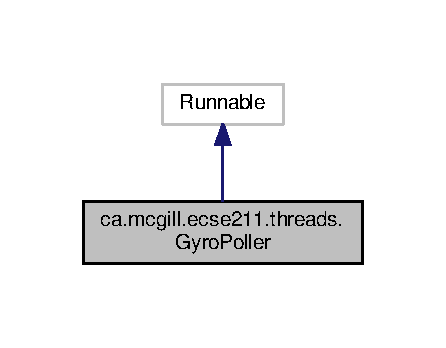
\includegraphics[width=214pt]{classca_1_1mcgill_1_1ecse211_1_1threads_1_1_gyro_poller__inherit__graph}
\end{center}
\end{figure}


Collaboration diagram for ca.\+mcgill.\+ecse211.\+threads.\+Gyro\+Poller\+:\nopagebreak
\begin{figure}[H]
\begin{center}
\leavevmode
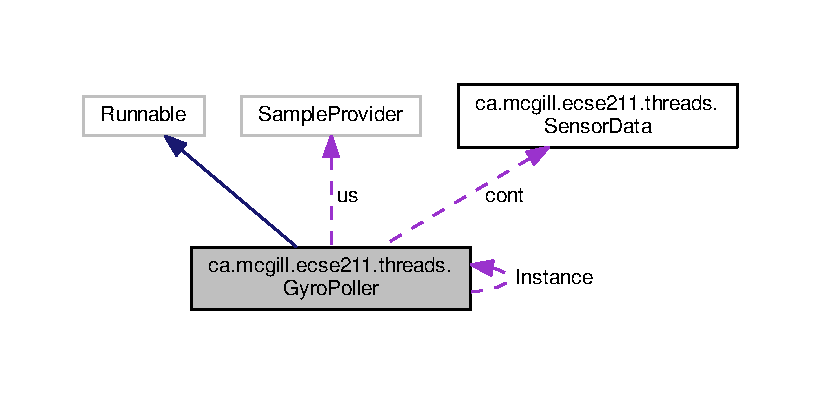
\includegraphics[width=350pt]{classca_1_1mcgill_1_1ecse211_1_1threads_1_1_gyro_poller__coll__graph}
\end{center}
\end{figure}
\subsection*{Public Member Functions}
\begin{DoxyCompactItemize}
\item 
\hyperlink{classca_1_1mcgill_1_1ecse211_1_1threads_1_1_gyro_poller_a1bab49cc19ee3b633ddbec4c408927bf}{Gyro\+Poller} (Sample\+Provider \hyperlink{classca_1_1mcgill_1_1ecse211_1_1threads_1_1_gyro_poller_af478329ec7a335a4f3d2d412d5d10091}{us}, float\mbox{[}$\,$\mbox{]} \hyperlink{classca_1_1mcgill_1_1ecse211_1_1threads_1_1_gyro_poller_a112e433b3561e89927357051f55f8cf1}{lg\+Data}, \hyperlink{classca_1_1mcgill_1_1ecse211_1_1threads_1_1_sensor_data}{Sensor\+Data} \hyperlink{classca_1_1mcgill_1_1ecse211_1_1threads_1_1_gyro_poller_a90507a3d6038ff7ec7881640b5dd4263}{cont})  throws Odometer\+Exceptions 
\item 
void \hyperlink{classca_1_1mcgill_1_1ecse211_1_1threads_1_1_gyro_poller_a7a3232e355cece714fa85a3a902d9cfd}{run} ()
\end{DoxyCompactItemize}
\subsection*{Public Attributes}
\begin{DoxyCompactItemize}
\item 
\hyperlink{classca_1_1mcgill_1_1ecse211_1_1threads_1_1_gyro_poller}{Gyro\+Poller} \hyperlink{classca_1_1mcgill_1_1ecse211_1_1threads_1_1_gyro_poller_a181979440aafff52b0ba5aaff9064f80}{Instance}
\end{DoxyCompactItemize}
\subsection*{Protected Member Functions}
\begin{DoxyCompactItemize}
\item 
void \hyperlink{classca_1_1mcgill_1_1ecse211_1_1threads_1_1_gyro_poller_a27f914ed77f23805210998fc0ee2daa7}{process\+Data} ()
\end{DoxyCompactItemize}
\subsection*{Protected Attributes}
\begin{DoxyCompactItemize}
\item 
Sample\+Provider \hyperlink{classca_1_1mcgill_1_1ecse211_1_1threads_1_1_gyro_poller_af478329ec7a335a4f3d2d412d5d10091}{us}
\item 
\hyperlink{classca_1_1mcgill_1_1ecse211_1_1threads_1_1_sensor_data}{Sensor\+Data} \hyperlink{classca_1_1mcgill_1_1ecse211_1_1threads_1_1_gyro_poller_a90507a3d6038ff7ec7881640b5dd4263}{cont}
\item 
float \mbox{[}$\,$\mbox{]} \hyperlink{classca_1_1mcgill_1_1ecse211_1_1threads_1_1_gyro_poller_a112e433b3561e89927357051f55f8cf1}{lg\+Data}
\end{DoxyCompactItemize}


\subsection{Detailed Description}
This class helps our robot to navigate using a gyroscope $<$Not using, deprecated$>$ \begin{DoxyAuthor}{Author}
Caspar Cedro 

Percy Chen 

Patrick Erath 

Anssam Ghezala 

Susan Matuszewski 

Kamy Moussavi Kafi 
\end{DoxyAuthor}


Definition at line 16 of file Gyro\+Poller.\+java.



\subsection{Constructor \& Destructor Documentation}
\mbox{\Hypertarget{classca_1_1mcgill_1_1ecse211_1_1threads_1_1_gyro_poller_a1bab49cc19ee3b633ddbec4c408927bf}\label{classca_1_1mcgill_1_1ecse211_1_1threads_1_1_gyro_poller_a1bab49cc19ee3b633ddbec4c408927bf}} 
\index{ca\+::mcgill\+::ecse211\+::threads\+::\+Gyro\+Poller@{ca\+::mcgill\+::ecse211\+::threads\+::\+Gyro\+Poller}!Gyro\+Poller@{Gyro\+Poller}}
\index{Gyro\+Poller@{Gyro\+Poller}!ca\+::mcgill\+::ecse211\+::threads\+::\+Gyro\+Poller@{ca\+::mcgill\+::ecse211\+::threads\+::\+Gyro\+Poller}}
\subsubsection{\texorpdfstring{Gyro\+Poller()}{GyroPoller()}}
{\footnotesize\ttfamily ca.\+mcgill.\+ecse211.\+threads.\+Gyro\+Poller.\+Gyro\+Poller (\begin{DoxyParamCaption}\item[{Sample\+Provider}]{us,  }\item[{float \mbox{[}$\,$\mbox{]}}]{lg\+Data,  }\item[{\hyperlink{classca_1_1mcgill_1_1ecse211_1_1threads_1_1_sensor_data}{Sensor\+Data}}]{cont }\end{DoxyParamCaption}) throws \hyperlink{classca_1_1mcgill_1_1ecse211_1_1odometer_1_1_odometer_exceptions}{Odometer\+Exceptions}}

This constructor creates an instance of the \hyperlink{classca_1_1mcgill_1_1ecse211_1_1threads_1_1_gyro_poller}{Gyro\+Poller} class to aid navigation


\begin{DoxyParams}{Parameters}
{\em us} & A Sample\+Provider class instance that helps us to store an array of ultrasonic sensor data. \\
\hline
{\em lg\+Data} & An array used to store data. \\
\hline
{\em cont} & A \hyperlink{classca_1_1mcgill_1_1ecse211_1_1threads_1_1_sensor_data}{Sensor\+Data} object instance used to manage sensor data. \\
\hline
\end{DoxyParams}

\begin{DoxyExceptions}{Exceptions}
{\em Odometer\+Exceptions} & \\
\hline
\end{DoxyExceptions}


Definition at line 31 of file Gyro\+Poller.\+java.


\begin{DoxyCode}
31                                                                                                   \{
32     this.\hyperlink{classca_1_1mcgill_1_1ecse211_1_1threads_1_1_gyro_poller_af478329ec7a335a4f3d2d412d5d10091}{us} = \hyperlink{classca_1_1mcgill_1_1ecse211_1_1threads_1_1_gyro_poller_af478329ec7a335a4f3d2d412d5d10091}{us};
33     this.\hyperlink{classca_1_1mcgill_1_1ecse211_1_1threads_1_1_gyro_poller_a90507a3d6038ff7ec7881640b5dd4263}{cont} = \hyperlink{classca_1_1mcgill_1_1ecse211_1_1threads_1_1_gyro_poller_a90507a3d6038ff7ec7881640b5dd4263}{cont};
34     this.\hyperlink{classca_1_1mcgill_1_1ecse211_1_1threads_1_1_gyro_poller_a112e433b3561e89927357051f55f8cf1}{lgData} = \hyperlink{classca_1_1mcgill_1_1ecse211_1_1threads_1_1_gyro_poller_a112e433b3561e89927357051f55f8cf1}{lgData};
35   \}
\end{DoxyCode}


\subsection{Member Function Documentation}
\mbox{\Hypertarget{classca_1_1mcgill_1_1ecse211_1_1threads_1_1_gyro_poller_a27f914ed77f23805210998fc0ee2daa7}\label{classca_1_1mcgill_1_1ecse211_1_1threads_1_1_gyro_poller_a27f914ed77f23805210998fc0ee2daa7}} 
\index{ca\+::mcgill\+::ecse211\+::threads\+::\+Gyro\+Poller@{ca\+::mcgill\+::ecse211\+::threads\+::\+Gyro\+Poller}!process\+Data@{process\+Data}}
\index{process\+Data@{process\+Data}!ca\+::mcgill\+::ecse211\+::threads\+::\+Gyro\+Poller@{ca\+::mcgill\+::ecse211\+::threads\+::\+Gyro\+Poller}}
\subsubsection{\texorpdfstring{process\+Data()}{processData()}}
{\footnotesize\ttfamily void ca.\+mcgill.\+ecse211.\+threads.\+Gyro\+Poller.\+process\+Data (\begin{DoxyParamCaption}{ }\end{DoxyParamCaption})\hspace{0.3cm}{\ttfamily [protected]}}



Definition at line 52 of file Gyro\+Poller.\+java.


\begin{DoxyCode}
52                                \{
53     \hyperlink{classca_1_1mcgill_1_1ecse211_1_1threads_1_1_gyro_poller_af478329ec7a335a4f3d2d412d5d10091}{us}.fetchSample(\hyperlink{classca_1_1mcgill_1_1ecse211_1_1threads_1_1_gyro_poller_a112e433b3561e89927357051f55f8cf1}{lgData}, 0); \textcolor{comment}{// acquire data}
54     \textcolor{keywordtype}{int} distance = (int) (\hyperlink{classca_1_1mcgill_1_1ecse211_1_1threads_1_1_gyro_poller_a112e433b3561e89927357051f55f8cf1}{lgData}[0]); \textcolor{comment}{// extract from buffer, cast to int}
55     \textcolor{comment}{// Ensure the distance is between 0 and 360}
56     \textcolor{keywordflow}{while} (distance < 0) \{
57       distance += 360;
58     \}
59 
60     \textcolor{keywordflow}{while} (distance > 360) \{
61       distance -= 360;
62     \}
63     \hyperlink{classca_1_1mcgill_1_1ecse211_1_1threads_1_1_gyro_poller_a90507a3d6038ff7ec7881640b5dd4263}{cont}.\hyperlink{classca_1_1mcgill_1_1ecse211_1_1threads_1_1_sensor_data_a35b1941d44e86b81eb7c625efbd3c8ba}{setA}(distance); \textcolor{comment}{// now take action depending on value}
64   \}
\end{DoxyCode}
Here is the call graph for this function\+:\nopagebreak
\begin{figure}[H]
\begin{center}
\leavevmode
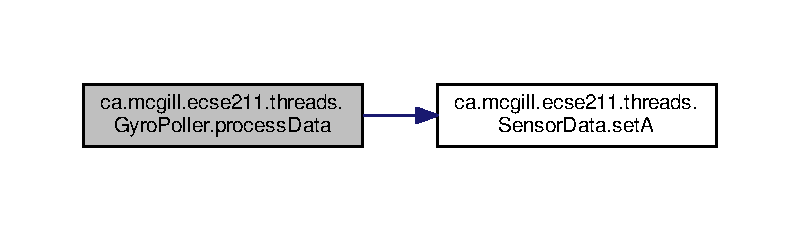
\includegraphics[width=350pt]{classca_1_1mcgill_1_1ecse211_1_1threads_1_1_gyro_poller_a27f914ed77f23805210998fc0ee2daa7_cgraph}
\end{center}
\end{figure}
Here is the caller graph for this function\+:\nopagebreak
\begin{figure}[H]
\begin{center}
\leavevmode
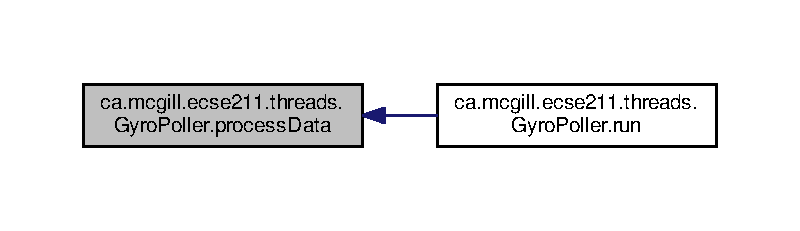
\includegraphics[width=350pt]{classca_1_1mcgill_1_1ecse211_1_1threads_1_1_gyro_poller_a27f914ed77f23805210998fc0ee2daa7_icgraph}
\end{center}
\end{figure}
\mbox{\Hypertarget{classca_1_1mcgill_1_1ecse211_1_1threads_1_1_gyro_poller_a7a3232e355cece714fa85a3a902d9cfd}\label{classca_1_1mcgill_1_1ecse211_1_1threads_1_1_gyro_poller_a7a3232e355cece714fa85a3a902d9cfd}} 
\index{ca\+::mcgill\+::ecse211\+::threads\+::\+Gyro\+Poller@{ca\+::mcgill\+::ecse211\+::threads\+::\+Gyro\+Poller}!run@{run}}
\index{run@{run}!ca\+::mcgill\+::ecse211\+::threads\+::\+Gyro\+Poller@{ca\+::mcgill\+::ecse211\+::threads\+::\+Gyro\+Poller}}
\subsubsection{\texorpdfstring{run()}{run()}}
{\footnotesize\ttfamily void ca.\+mcgill.\+ecse211.\+threads.\+Gyro\+Poller.\+run (\begin{DoxyParamCaption}{ }\end{DoxyParamCaption})}

This method is called by a \hyperlink{classca_1_1mcgill_1_1ecse211_1_1threads_1_1_ultrasonic_poller}{Ultrasonic\+Poller} (Thread) instance when it is asked to start executing

Sensors now return floats using a uniform protocol. Need to convert US result to an integer \mbox{[}0,255\mbox{]} (non-\/\+Javadoc)

\begin{DoxySeeAlso}{See also}
java.\+lang.\+Thread\+::run() 
\end{DoxySeeAlso}


Definition at line 46 of file Gyro\+Poller.\+java.


\begin{DoxyCode}
46                     \{
47     \textcolor{keywordflow}{while} (\textcolor{keyword}{true}) \{
48       \hyperlink{classca_1_1mcgill_1_1ecse211_1_1threads_1_1_gyro_poller_a27f914ed77f23805210998fc0ee2daa7}{processData}();
49     \}
50   \}
\end{DoxyCode}
Here is the call graph for this function\+:\nopagebreak
\begin{figure}[H]
\begin{center}
\leavevmode
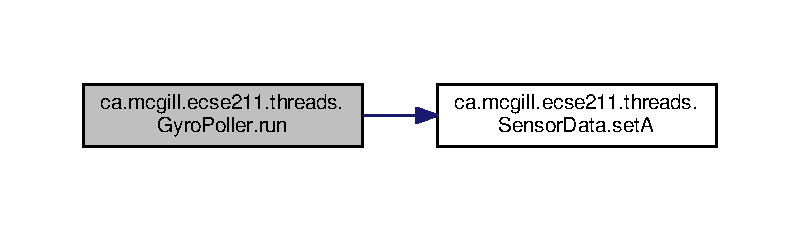
\includegraphics[width=350pt]{classca_1_1mcgill_1_1ecse211_1_1threads_1_1_gyro_poller_a7a3232e355cece714fa85a3a902d9cfd_cgraph}
\end{center}
\end{figure}


\subsection{Member Data Documentation}
\mbox{\Hypertarget{classca_1_1mcgill_1_1ecse211_1_1threads_1_1_gyro_poller_a90507a3d6038ff7ec7881640b5dd4263}\label{classca_1_1mcgill_1_1ecse211_1_1threads_1_1_gyro_poller_a90507a3d6038ff7ec7881640b5dd4263}} 
\index{ca\+::mcgill\+::ecse211\+::threads\+::\+Gyro\+Poller@{ca\+::mcgill\+::ecse211\+::threads\+::\+Gyro\+Poller}!cont@{cont}}
\index{cont@{cont}!ca\+::mcgill\+::ecse211\+::threads\+::\+Gyro\+Poller@{ca\+::mcgill\+::ecse211\+::threads\+::\+Gyro\+Poller}}
\subsubsection{\texorpdfstring{cont}{cont}}
{\footnotesize\ttfamily \hyperlink{classca_1_1mcgill_1_1ecse211_1_1threads_1_1_sensor_data}{Sensor\+Data} ca.\+mcgill.\+ecse211.\+threads.\+Gyro\+Poller.\+cont\hspace{0.3cm}{\ttfamily [protected]}}



Definition at line 18 of file Gyro\+Poller.\+java.

\mbox{\Hypertarget{classca_1_1mcgill_1_1ecse211_1_1threads_1_1_gyro_poller_a181979440aafff52b0ba5aaff9064f80}\label{classca_1_1mcgill_1_1ecse211_1_1threads_1_1_gyro_poller_a181979440aafff52b0ba5aaff9064f80}} 
\index{ca\+::mcgill\+::ecse211\+::threads\+::\+Gyro\+Poller@{ca\+::mcgill\+::ecse211\+::threads\+::\+Gyro\+Poller}!Instance@{Instance}}
\index{Instance@{Instance}!ca\+::mcgill\+::ecse211\+::threads\+::\+Gyro\+Poller@{ca\+::mcgill\+::ecse211\+::threads\+::\+Gyro\+Poller}}
\subsubsection{\texorpdfstring{Instance}{Instance}}
{\footnotesize\ttfamily \hyperlink{classca_1_1mcgill_1_1ecse211_1_1threads_1_1_gyro_poller}{Gyro\+Poller} ca.\+mcgill.\+ecse211.\+threads.\+Gyro\+Poller.\+Instance}



Definition at line 20 of file Gyro\+Poller.\+java.

\mbox{\Hypertarget{classca_1_1mcgill_1_1ecse211_1_1threads_1_1_gyro_poller_a112e433b3561e89927357051f55f8cf1}\label{classca_1_1mcgill_1_1ecse211_1_1threads_1_1_gyro_poller_a112e433b3561e89927357051f55f8cf1}} 
\index{ca\+::mcgill\+::ecse211\+::threads\+::\+Gyro\+Poller@{ca\+::mcgill\+::ecse211\+::threads\+::\+Gyro\+Poller}!lg\+Data@{lg\+Data}}
\index{lg\+Data@{lg\+Data}!ca\+::mcgill\+::ecse211\+::threads\+::\+Gyro\+Poller@{ca\+::mcgill\+::ecse211\+::threads\+::\+Gyro\+Poller}}
\subsubsection{\texorpdfstring{lg\+Data}{lgData}}
{\footnotesize\ttfamily float \mbox{[}$\,$\mbox{]} ca.\+mcgill.\+ecse211.\+threads.\+Gyro\+Poller.\+lg\+Data\hspace{0.3cm}{\ttfamily [protected]}}



Definition at line 19 of file Gyro\+Poller.\+java.

\mbox{\Hypertarget{classca_1_1mcgill_1_1ecse211_1_1threads_1_1_gyro_poller_af478329ec7a335a4f3d2d412d5d10091}\label{classca_1_1mcgill_1_1ecse211_1_1threads_1_1_gyro_poller_af478329ec7a335a4f3d2d412d5d10091}} 
\index{ca\+::mcgill\+::ecse211\+::threads\+::\+Gyro\+Poller@{ca\+::mcgill\+::ecse211\+::threads\+::\+Gyro\+Poller}!us@{us}}
\index{us@{us}!ca\+::mcgill\+::ecse211\+::threads\+::\+Gyro\+Poller@{ca\+::mcgill\+::ecse211\+::threads\+::\+Gyro\+Poller}}
\subsubsection{\texorpdfstring{us}{us}}
{\footnotesize\ttfamily Sample\+Provider ca.\+mcgill.\+ecse211.\+threads.\+Gyro\+Poller.\+us\hspace{0.3cm}{\ttfamily [protected]}}



Definition at line 17 of file Gyro\+Poller.\+java.



The documentation for this class was generated from the following file\+:\begin{DoxyCompactItemize}
\item 
/home/ccc/\+Final\+Project/src/ca/mcgill/ecse211/threads/\hyperlink{_gyro_poller_8java}{Gyro\+Poller.\+java}\end{DoxyCompactItemize}

\hypertarget{classca_1_1mcgill_1_1ecse211_1_1localization_1_1_light_localizer}{}\section{ca.\+mcgill.\+ecse211.\+localization.\+Light\+Localizer Class Reference}
\label{classca_1_1mcgill_1_1ecse211_1_1localization_1_1_light_localizer}\index{ca.\+mcgill.\+ecse211.\+localization.\+Light\+Localizer@{ca.\+mcgill.\+ecse211.\+localization.\+Light\+Localizer}}
\subsection*{Public Member Functions}
\begin{DoxyCompactItemize}
\item 
\hyperlink{classca_1_1mcgill_1_1ecse211_1_1localization_1_1_light_localizer_aa37a75b7c32c02fe261845021f0734b7}{Light\+Localizer} (\hyperlink{classca_1_1mcgill_1_1ecse211_1_1project_1_1_navigation}{Navigation} nav, E\+V3\+Large\+Regulated\+Motor left\+Motor, E\+V3\+Large\+Regulated\+Motor right\+Motor)  throws Odometer\+Exceptions 
\item 
void \hyperlink{classca_1_1mcgill_1_1ecse211_1_1localization_1_1_light_localizer_a9fc3d6cdd897e9db86fc9d71dc914863}{localize} (int\mbox{[}$\,$\mbox{]} sC)
\end{DoxyCompactItemize}


\subsection{Detailed Description}
This class helps our robot to localize itself using the light sensor

\begin{DoxyAuthor}{Author}
Caspar Cedro 

Percy Chen 

Patrick Erath 

Anssam Ghezala 

Susan Matuszewski 

Kamy Moussavi Kafi 
\end{DoxyAuthor}


Definition at line 21 of file Light\+Localizer.\+java.



\subsection{Constructor \& Destructor Documentation}
\mbox{\Hypertarget{classca_1_1mcgill_1_1ecse211_1_1localization_1_1_light_localizer_aa37a75b7c32c02fe261845021f0734b7}\label{classca_1_1mcgill_1_1ecse211_1_1localization_1_1_light_localizer_aa37a75b7c32c02fe261845021f0734b7}} 
\index{ca\+::mcgill\+::ecse211\+::localization\+::\+Light\+Localizer@{ca\+::mcgill\+::ecse211\+::localization\+::\+Light\+Localizer}!Light\+Localizer@{Light\+Localizer}}
\index{Light\+Localizer@{Light\+Localizer}!ca\+::mcgill\+::ecse211\+::localization\+::\+Light\+Localizer@{ca\+::mcgill\+::ecse211\+::localization\+::\+Light\+Localizer}}
\subsubsection{\texorpdfstring{Light\+Localizer()}{LightLocalizer()}}
{\footnotesize\ttfamily ca.\+mcgill.\+ecse211.\+localization.\+Light\+Localizer.\+Light\+Localizer (\begin{DoxyParamCaption}\item[{\hyperlink{classca_1_1mcgill_1_1ecse211_1_1project_1_1_navigation}{Navigation}}]{nav,  }\item[{E\+V3\+Large\+Regulated\+Motor}]{left\+Motor,  }\item[{E\+V3\+Large\+Regulated\+Motor}]{right\+Motor }\end{DoxyParamCaption}) throws \hyperlink{classca_1_1mcgill_1_1ecse211_1_1odometer_1_1_odometer_exceptions}{Odometer\+Exceptions}}

This is the class constructor


\begin{DoxyParams}{Parameters}
{\em left\+Motor} & \\
\hline
{\em right\+Motor} & \\
\hline
\end{DoxyParams}

\begin{DoxyExceptions}{Exceptions}
{\em Odometer\+Exceptions} & \\
\hline
\end{DoxyExceptions}


Definition at line 38 of file Light\+Localizer.\+java.


\begin{DoxyCode}
39                                                                    \{
40     this.odometer = Odometer.\hyperlink{classca_1_1mcgill_1_1ecse211_1_1odometer_1_1_odometer_a99171f11e34dea918fa9dd069d721439}{getOdometer}();
41     this.data = SensorData.\hyperlink{classca_1_1mcgill_1_1ecse211_1_1threads_1_1_sensor_data_a8260aba53b4474ca1275e4ce26157977}{getSensorData}();
42     this.navigation = nav;
43     this.leftMotor = leftMotor;
44     this.rightMotor = rightMotor;
45   \}
\end{DoxyCode}
Here is the call graph for this function\+:\nopagebreak
\begin{figure}[H]
\begin{center}
\leavevmode
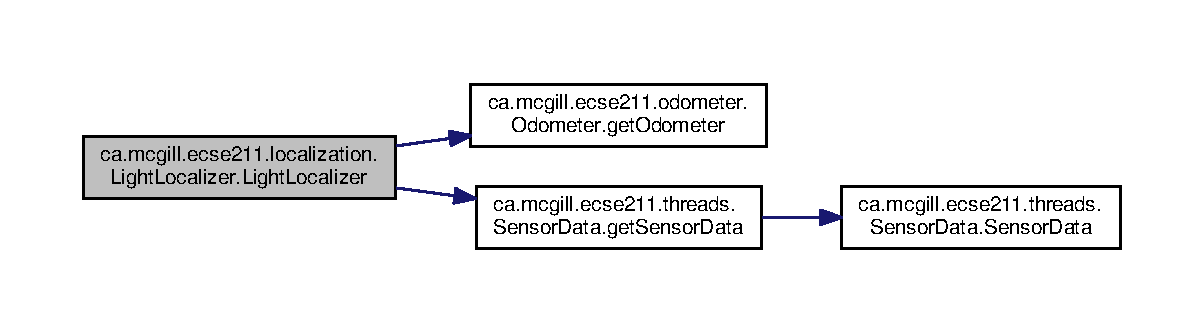
\includegraphics[width=350pt]{classca_1_1mcgill_1_1ecse211_1_1localization_1_1_light_localizer_aa37a75b7c32c02fe261845021f0734b7_cgraph}
\end{center}
\end{figure}


\subsection{Member Function Documentation}
\mbox{\Hypertarget{classca_1_1mcgill_1_1ecse211_1_1localization_1_1_light_localizer_a9fc3d6cdd897e9db86fc9d71dc914863}\label{classca_1_1mcgill_1_1ecse211_1_1localization_1_1_light_localizer_a9fc3d6cdd897e9db86fc9d71dc914863}} 
\index{ca\+::mcgill\+::ecse211\+::localization\+::\+Light\+Localizer@{ca\+::mcgill\+::ecse211\+::localization\+::\+Light\+Localizer}!localize@{localize}}
\index{localize@{localize}!ca\+::mcgill\+::ecse211\+::localization\+::\+Light\+Localizer@{ca\+::mcgill\+::ecse211\+::localization\+::\+Light\+Localizer}}
\subsubsection{\texorpdfstring{localize()}{localize()}}
{\footnotesize\ttfamily void ca.\+mcgill.\+ecse211.\+localization.\+Light\+Localizer.\+localize (\begin{DoxyParamCaption}\item[{int \mbox{[}$\,$\mbox{]}}]{sC }\end{DoxyParamCaption})}

({\itshape Improve}) Once the robot know what angle it is facing, this method looks for the x,y axis origins knowing it is in the first tile facing north. 
\begin{DoxyParams}{Parameters}
{\em sC} & the coordinate to set to after localization \\
\hline
\end{DoxyParams}


Definition at line 53 of file Light\+Localizer.\+java.


\begin{DoxyCode}
53                                  \{
54     leftMotor.setSpeed(FORWARD\_SPEED);
55     rightMotor.setSpeed(FORWARD\_SPEED);
56 
57     \textcolor{comment}{// 1. GO forward find the y=0 line}
58     leftMotor.forward();
59     rightMotor.forward();
60     \textcolor{keywordflow}{while} (data.\hyperlink{classca_1_1mcgill_1_1ecse211_1_1threads_1_1_sensor_data_a39eec50582f0e4bcff8a4669c48e1609}{getL}()[0] > blackLineColor);
61     Sound.beep();
62     odometer.\hyperlink{classca_1_1mcgill_1_1ecse211_1_1odometer_1_1_odometer_data_a82986438cd462e66520bc62bb4bd2b75}{setY}(0);
63     \textcolor{comment}{// 2. Turn and go forward find the x=0 line}
64     navigation.\hyperlink{classca_1_1mcgill_1_1ecse211_1_1project_1_1_navigation_a3bbe0645f2b3b3d0986b4a707fb5a00c}{turnTo}(90);
65     leftMotor.setSpeed(FORWARD\_SPEED / 2);
66     rightMotor.setSpeed(FORWARD\_SPEED / 2);
67     leftMotor.forward();
68     rightMotor.forward();
69     \textcolor{keywordflow}{while} (data.\hyperlink{classca_1_1mcgill_1_1ecse211_1_1threads_1_1_sensor_data_a39eec50582f0e4bcff8a4669c48e1609}{getL}()[0] > blackLineColor);
70     Sound.beep();
71     odometer.\hyperlink{classca_1_1mcgill_1_1ecse211_1_1odometer_1_1_odometer_data_a2911d7215e47f3064defe016b46bfeef}{setX}(0);
72     leftMotor.setSpeed(FORWARD\_SPEED / 2);
73     rightMotor.setSpeed(FORWARD\_SPEED / 2);
74     \textcolor{comment}{// 3. Go backwards by sensor-wheel center distance in x-direction}
75     leftMotor.rotate(Navigation.convertDistance(Game.WHEEL\_RAD, -SENSOR\_DIS), \textcolor{keyword}{true});
76     rightMotor.rotate(Navigation.convertDistance(Game.WHEEL\_RAD, -SENSOR\_DIS), \textcolor{keyword}{false});
77     \textcolor{comment}{// 4. Go backwards by sensor-wheel center distance in y-direction}
78     navigation.\hyperlink{classca_1_1mcgill_1_1ecse211_1_1project_1_1_navigation_a3bbe0645f2b3b3d0986b4a707fb5a00c}{turnTo}(0);
79     leftMotor.setSpeed(FORWARD\_SPEED / 2);
80     rightMotor.setSpeed(FORWARD\_SPEED / 2);
81     \textcolor{keywordtype}{double} sensorDistanceOffset = 2.5;
82     leftMotor.rotate(
83         Navigation.convertDistance(Game.WHEEL\_RAD, -SENSOR\_DIS - sensorDistanceOffset),
84         \textcolor{keyword}{true});
85     rightMotor.rotate(
86         Navigation.convertDistance(Game.WHEEL\_RAD, -SENSOR\_DIS - sensorDistanceOffset),
87         \textcolor{keyword}{false});
88     odometer.\hyperlink{classca_1_1mcgill_1_1ecse211_1_1odometer_1_1_odometer_data_a419b8f07c2c5374411c8e62298e9a402}{setTheta}(0);
89     odometer.\hyperlink{classca_1_1mcgill_1_1ecse211_1_1odometer_1_1_odometer_data_a2911d7215e47f3064defe016b46bfeef}{setX}(sC[0]);
90     odometer.\hyperlink{classca_1_1mcgill_1_1ecse211_1_1odometer_1_1_odometer_data_a82986438cd462e66520bc62bb4bd2b75}{setY}(sC[1]);
91 
92   \}
\end{DoxyCode}
Here is the call graph for this function\+:\nopagebreak
\begin{figure}[H]
\begin{center}
\leavevmode
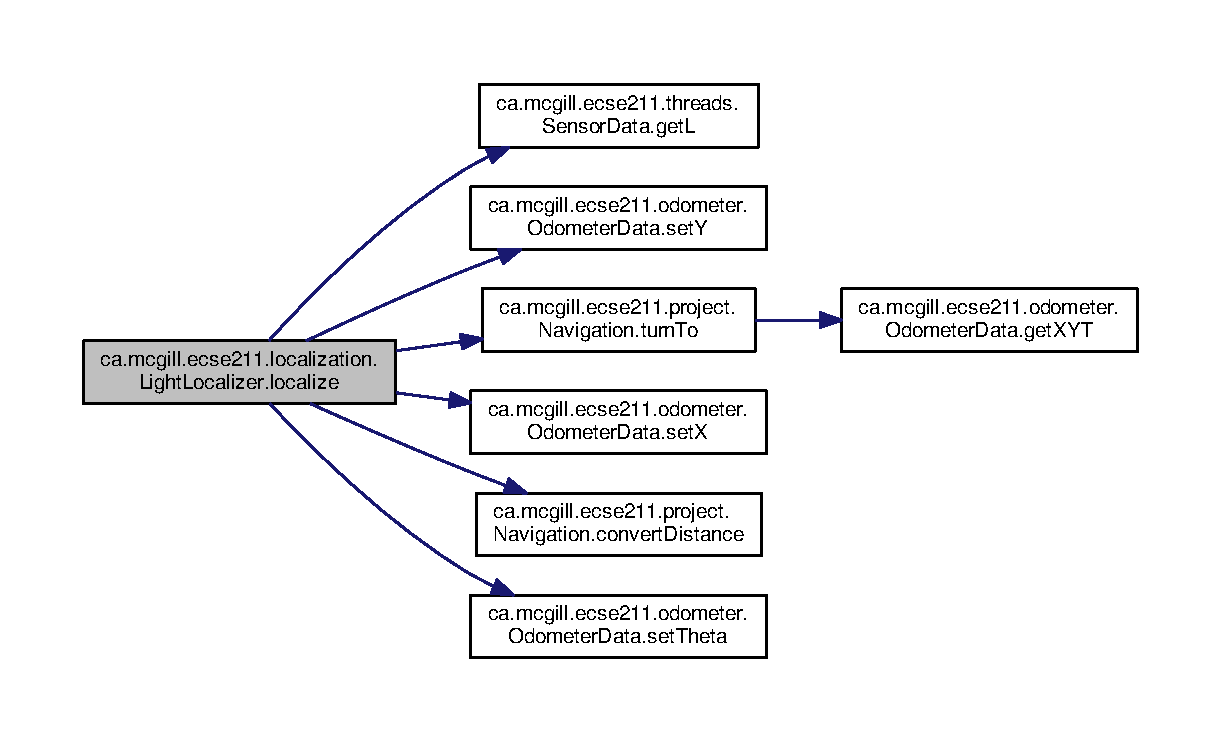
\includegraphics[width=350pt]{classca_1_1mcgill_1_1ecse211_1_1localization_1_1_light_localizer_a9fc3d6cdd897e9db86fc9d71dc914863_cgraph}
\end{center}
\end{figure}
Here is the caller graph for this function\+:
\nopagebreak
\begin{figure}[H]
\begin{center}
\leavevmode
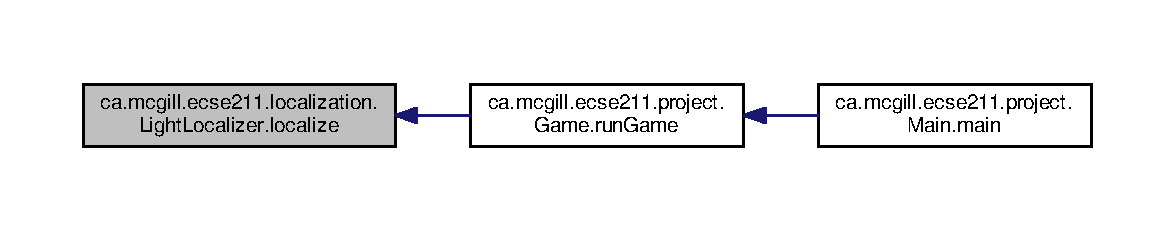
\includegraphics[width=350pt]{classca_1_1mcgill_1_1ecse211_1_1localization_1_1_light_localizer_a9fc3d6cdd897e9db86fc9d71dc914863_icgraph}
\end{center}
\end{figure}


The documentation for this class was generated from the following file\+:\begin{DoxyCompactItemize}
\item 
/home/ccc/\+Final\+Project/src/ca/mcgill/ecse211/localization/\hyperlink{_light_localizer_8java}{Light\+Localizer.\+java}\end{DoxyCompactItemize}

\hypertarget{classca_1_1mcgill_1_1ecse211_1_1threads_1_1_light_poller}{}\section{ca.\+mcgill.\+ecse211.\+threads.\+Light\+Poller Class Reference}
\label{classca_1_1mcgill_1_1ecse211_1_1threads_1_1_light_poller}\index{ca.\+mcgill.\+ecse211.\+threads.\+Light\+Poller@{ca.\+mcgill.\+ecse211.\+threads.\+Light\+Poller}}


Inheritance diagram for ca.\+mcgill.\+ecse211.\+threads.\+Light\+Poller\+:\nopagebreak
\begin{figure}[H]
\begin{center}
\leavevmode
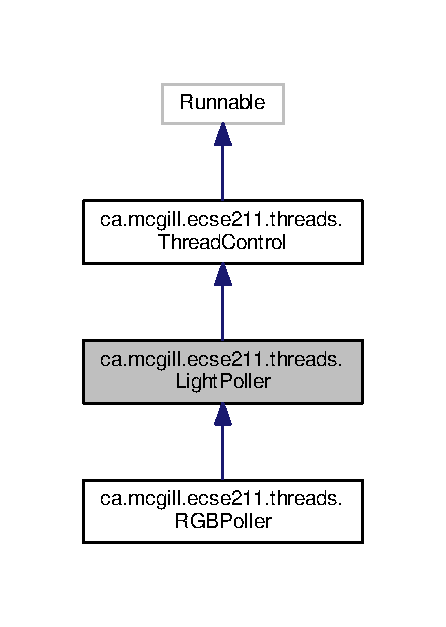
\includegraphics[width=214pt]{classca_1_1mcgill_1_1ecse211_1_1threads_1_1_light_poller__inherit__graph}
\end{center}
\end{figure}


Collaboration diagram for ca.\+mcgill.\+ecse211.\+threads.\+Light\+Poller\+:\nopagebreak
\begin{figure}[H]
\begin{center}
\leavevmode
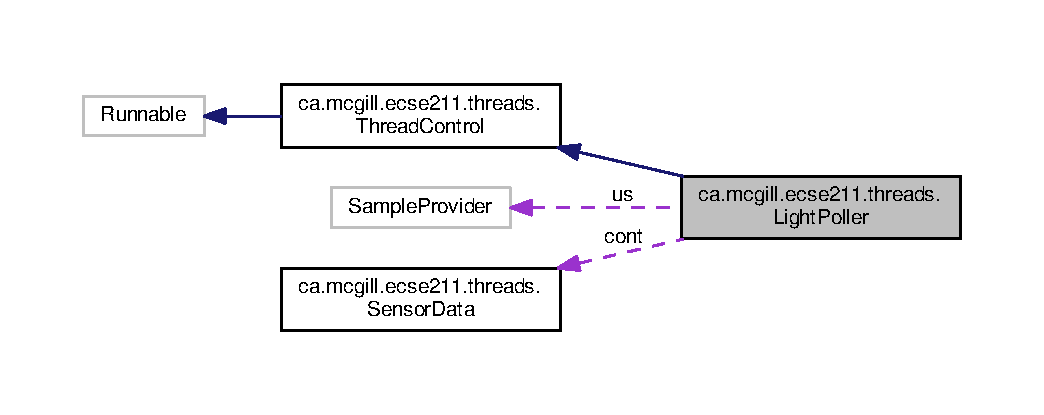
\includegraphics[width=350pt]{classca_1_1mcgill_1_1ecse211_1_1threads_1_1_light_poller__coll__graph}
\end{center}
\end{figure}
\subsection*{Public Member Functions}
\begin{DoxyCompactItemize}
\item 
\hyperlink{classca_1_1mcgill_1_1ecse211_1_1threads_1_1_light_poller_adc07f842a1cc089195c5e47c2a0e5ee6}{Light\+Poller} (Sample\+Provider\mbox{[}$\,$\mbox{]} \hyperlink{classca_1_1mcgill_1_1ecse211_1_1threads_1_1_light_poller_ab6a9cb770bbf71f586697633db1475ff}{us}, float\mbox{[}$\,$\mbox{]}\mbox{[}$\,$\mbox{]} \hyperlink{classca_1_1mcgill_1_1ecse211_1_1threads_1_1_light_poller_a6cf53aecc3efc481f71d36341d2276c6}{lg\+Data}, \hyperlink{classca_1_1mcgill_1_1ecse211_1_1threads_1_1_sensor_data}{Sensor\+Data} \hyperlink{classca_1_1mcgill_1_1ecse211_1_1threads_1_1_light_poller_ab6a9050ced4f6940add4735c8872194a}{cont})  throws Odometer\+Exceptions 
\end{DoxyCompactItemize}
\subsection*{Protected Member Functions}
\begin{DoxyCompactItemize}
\item 
void \hyperlink{classca_1_1mcgill_1_1ecse211_1_1threads_1_1_light_poller_aab90a460a4d0c926fb8f3930492a8fb1}{run\+Method} ()
\end{DoxyCompactItemize}
\subsection*{Protected Attributes}
\begin{DoxyCompactItemize}
\item 
Sample\+Provider \hyperlink{classca_1_1mcgill_1_1ecse211_1_1threads_1_1_light_poller_ab6a9cb770bbf71f586697633db1475ff}{us} \mbox{[}$\,$\mbox{]}
\item 
\hyperlink{classca_1_1mcgill_1_1ecse211_1_1threads_1_1_sensor_data}{Sensor\+Data} \hyperlink{classca_1_1mcgill_1_1ecse211_1_1threads_1_1_light_poller_ab6a9050ced4f6940add4735c8872194a}{cont}
\item 
float \mbox{[}$\,$\mbox{]}\mbox{[}$\,$\mbox{]} \hyperlink{classca_1_1mcgill_1_1ecse211_1_1threads_1_1_light_poller_a6cf53aecc3efc481f71d36341d2276c6}{lg\+Data}
\item 
float \hyperlink{classca_1_1mcgill_1_1ecse211_1_1threads_1_1_light_poller_a79908bf56395ae82ab5ac57b5b40f206}{last\+Value} \mbox{[}$\,$\mbox{]}
\end{DoxyCompactItemize}
\subsection*{Additional Inherited Members}


\subsection{Detailed Description}
This class implements the Light Sensor Poller for our robot it runs pulls the sensor data every 50 miliseconds \begin{DoxyAuthor}{Author}
Caspar Cedro 

Percy Chen 

Patrick Erath 

Anssam Ghezala 

Susan Matuszewski 

Kamy Moussavi Kafi 
\end{DoxyAuthor}


Definition at line 16 of file Light\+Poller.\+java.



\subsection{Constructor \& Destructor Documentation}
\mbox{\Hypertarget{classca_1_1mcgill_1_1ecse211_1_1threads_1_1_light_poller_adc07f842a1cc089195c5e47c2a0e5ee6}\label{classca_1_1mcgill_1_1ecse211_1_1threads_1_1_light_poller_adc07f842a1cc089195c5e47c2a0e5ee6}} 
\index{ca\+::mcgill\+::ecse211\+::threads\+::\+Light\+Poller@{ca\+::mcgill\+::ecse211\+::threads\+::\+Light\+Poller}!Light\+Poller@{Light\+Poller}}
\index{Light\+Poller@{Light\+Poller}!ca\+::mcgill\+::ecse211\+::threads\+::\+Light\+Poller@{ca\+::mcgill\+::ecse211\+::threads\+::\+Light\+Poller}}
\subsubsection{\texorpdfstring{Light\+Poller()}{LightPoller()}}
{\footnotesize\ttfamily ca.\+mcgill.\+ecse211.\+threads.\+Light\+Poller.\+Light\+Poller (\begin{DoxyParamCaption}\item[{Sample\+Provider \mbox{[}$\,$\mbox{]}}]{us,  }\item[{float}]{lg\+Data\mbox{[}$\,$\mbox{]}\mbox{[}$\,$\mbox{]},  }\item[{\hyperlink{classca_1_1mcgill_1_1ecse211_1_1threads_1_1_sensor_data}{Sensor\+Data}}]{cont }\end{DoxyParamCaption}) throws \hyperlink{classca_1_1mcgill_1_1ecse211_1_1odometer_1_1_odometer_exceptions}{Odometer\+Exceptions}}

This constructor creates an instance of the \hyperlink{classca_1_1mcgill_1_1ecse211_1_1threads_1_1_light_poller}{Light\+Poller} class to provide distance data from an light sensor to our robot.


\begin{DoxyParams}{Parameters}
{\em us} & a Sample\+Provider class instance that helps us to store an array of ultrasonic sensor data. \\
\hline
{\em lg\+Data} & an array of distance data to be used by our Wall Follower\textquotesingle{}s Ultrasonic\+Controllers. \\
\hline
{\em cont} & a Bang\+Bang\+Controller or P\+Controller instance that has accumulated distance data stored in us\+Data passed to it. \\
\hline
\end{DoxyParams}

\begin{DoxyExceptions}{Exceptions}
{\em Odometer\+Exceptions} & \\
\hline
\end{DoxyExceptions}


Definition at line 35 of file Light\+Poller.\+java.


\begin{DoxyCode}
35                                                                                                        \{
36     this.\hyperlink{classca_1_1mcgill_1_1ecse211_1_1threads_1_1_light_poller_ab6a9cb770bbf71f586697633db1475ff}{us} = \hyperlink{classca_1_1mcgill_1_1ecse211_1_1threads_1_1_light_poller_ab6a9cb770bbf71f586697633db1475ff}{us};
37     this.\hyperlink{classca_1_1mcgill_1_1ecse211_1_1threads_1_1_light_poller_ab6a9050ced4f6940add4735c8872194a}{cont} = \hyperlink{classca_1_1mcgill_1_1ecse211_1_1threads_1_1_light_poller_ab6a9050ced4f6940add4735c8872194a}{cont};
38     this.\hyperlink{classca_1_1mcgill_1_1ecse211_1_1threads_1_1_light_poller_a6cf53aecc3efc481f71d36341d2276c6}{lgData} = \hyperlink{classca_1_1mcgill_1_1ecse211_1_1threads_1_1_light_poller_a6cf53aecc3efc481f71d36341d2276c6}{lgData};
39     \hyperlink{classca_1_1mcgill_1_1ecse211_1_1threads_1_1_thread_control_a92f4933511db42476e39956246bcf2fe}{isStarted} = \textcolor{keyword}{true};
40     \hyperlink{classca_1_1mcgill_1_1ecse211_1_1threads_1_1_light_poller_a79908bf56395ae82ab5ac57b5b40f206}{lastValue} = \textcolor{keyword}{new} \textcolor{keywordtype}{float}[2];
41     sensorNumber++;
42     \hyperlink{classca_1_1mcgill_1_1ecse211_1_1threads_1_1_thread_control_a395cfe1d73b3ef14da0830ed0a499f82}{WAIT\_TIME} = 50;
43   \}
\end{DoxyCode}
Here is the call graph for this function\+:\nopagebreak
\begin{figure}[H]
\begin{center}
\leavevmode
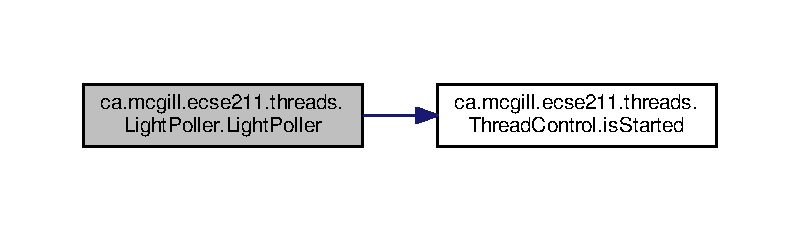
\includegraphics[width=350pt]{classca_1_1mcgill_1_1ecse211_1_1threads_1_1_light_poller_adc07f842a1cc089195c5e47c2a0e5ee6_cgraph}
\end{center}
\end{figure}


\subsection{Member Function Documentation}
\mbox{\Hypertarget{classca_1_1mcgill_1_1ecse211_1_1threads_1_1_light_poller_aab90a460a4d0c926fb8f3930492a8fb1}\label{classca_1_1mcgill_1_1ecse211_1_1threads_1_1_light_poller_aab90a460a4d0c926fb8f3930492a8fb1}} 
\index{ca\+::mcgill\+::ecse211\+::threads\+::\+Light\+Poller@{ca\+::mcgill\+::ecse211\+::threads\+::\+Light\+Poller}!run\+Method@{run\+Method}}
\index{run\+Method@{run\+Method}!ca\+::mcgill\+::ecse211\+::threads\+::\+Light\+Poller@{ca\+::mcgill\+::ecse211\+::threads\+::\+Light\+Poller}}
\subsubsection{\texorpdfstring{run\+Method()}{runMethod()}}
{\footnotesize\ttfamily void ca.\+mcgill.\+ecse211.\+threads.\+Light\+Poller.\+run\+Method (\begin{DoxyParamCaption}{ }\end{DoxyParamCaption})\hspace{0.3cm}{\ttfamily [protected]}}

the run method to be performed in run method, collect light data 

Definition at line 48 of file Light\+Poller.\+java.


\begin{DoxyCode}
48                              \{
49     \textcolor{keywordtype}{double} l[] = \textcolor{keyword}{new} \textcolor{keywordtype}{double}[2];
50     \textcolor{keywordflow}{for}(\textcolor{keywordtype}{int} i = 0; i < \hyperlink{classca_1_1mcgill_1_1ecse211_1_1threads_1_1_light_poller_ab6a9cb770bbf71f586697633db1475ff}{us}.length; i++) \{
51       \hyperlink{classca_1_1mcgill_1_1ecse211_1_1threads_1_1_light_poller_ab6a9cb770bbf71f586697633db1475ff}{us}[i].fetchSample(\hyperlink{classca_1_1mcgill_1_1ecse211_1_1threads_1_1_light_poller_a6cf53aecc3efc481f71d36341d2276c6}{lgData}[i], 0); \textcolor{comment}{// acquire data}
52   
53       \textcolor{keywordtype}{int} distance = (int) (\hyperlink{classca_1_1mcgill_1_1ecse211_1_1threads_1_1_light_poller_a6cf53aecc3efc481f71d36341d2276c6}{lgData}[i][0] * 100); \textcolor{comment}{// extract from buffer, multiply by 100 for
       convenience}
54                                               \textcolor{comment}{// and allow it to be cast to int}
55       l[i] = distance - \hyperlink{classca_1_1mcgill_1_1ecse211_1_1threads_1_1_light_poller_a79908bf56395ae82ab5ac57b5b40f206}{lastValue}[i]; \textcolor{comment}{// now take action depending on value}
56       lastValue[i] = distance; 
57     \}
58     \hyperlink{classca_1_1mcgill_1_1ecse211_1_1threads_1_1_light_poller_ab6a9050ced4f6940add4735c8872194a}{cont}.\hyperlink{classca_1_1mcgill_1_1ecse211_1_1threads_1_1_sensor_data_af905a6f2825716ae1a39bf7f6be09477}{setL}(l);
59   \}
\end{DoxyCode}
Here is the call graph for this function\+:\nopagebreak
\begin{figure}[H]
\begin{center}
\leavevmode
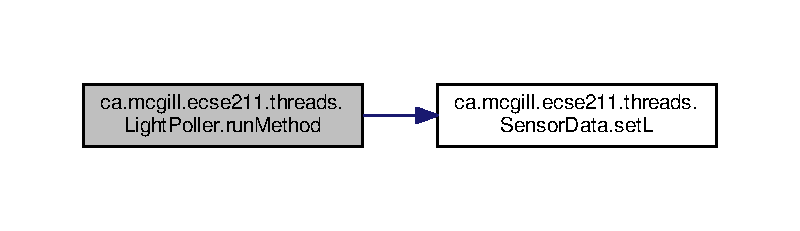
\includegraphics[width=350pt]{classca_1_1mcgill_1_1ecse211_1_1threads_1_1_light_poller_aab90a460a4d0c926fb8f3930492a8fb1_cgraph}
\end{center}
\end{figure}


\subsection{Member Data Documentation}
\mbox{\Hypertarget{classca_1_1mcgill_1_1ecse211_1_1threads_1_1_light_poller_ab6a9050ced4f6940add4735c8872194a}\label{classca_1_1mcgill_1_1ecse211_1_1threads_1_1_light_poller_ab6a9050ced4f6940add4735c8872194a}} 
\index{ca\+::mcgill\+::ecse211\+::threads\+::\+Light\+Poller@{ca\+::mcgill\+::ecse211\+::threads\+::\+Light\+Poller}!cont@{cont}}
\index{cont@{cont}!ca\+::mcgill\+::ecse211\+::threads\+::\+Light\+Poller@{ca\+::mcgill\+::ecse211\+::threads\+::\+Light\+Poller}}
\subsubsection{\texorpdfstring{cont}{cont}}
{\footnotesize\ttfamily \hyperlink{classca_1_1mcgill_1_1ecse211_1_1threads_1_1_sensor_data}{Sensor\+Data} ca.\+mcgill.\+ecse211.\+threads.\+Light\+Poller.\+cont\hspace{0.3cm}{\ttfamily [protected]}}



Definition at line 18 of file Light\+Poller.\+java.

\mbox{\Hypertarget{classca_1_1mcgill_1_1ecse211_1_1threads_1_1_light_poller_a79908bf56395ae82ab5ac57b5b40f206}\label{classca_1_1mcgill_1_1ecse211_1_1threads_1_1_light_poller_a79908bf56395ae82ab5ac57b5b40f206}} 
\index{ca\+::mcgill\+::ecse211\+::threads\+::\+Light\+Poller@{ca\+::mcgill\+::ecse211\+::threads\+::\+Light\+Poller}!last\+Value@{last\+Value}}
\index{last\+Value@{last\+Value}!ca\+::mcgill\+::ecse211\+::threads\+::\+Light\+Poller@{ca\+::mcgill\+::ecse211\+::threads\+::\+Light\+Poller}}
\subsubsection{\texorpdfstring{last\+Value}{lastValue}}
{\footnotesize\ttfamily float ca.\+mcgill.\+ecse211.\+threads.\+Light\+Poller.\+last\+Value\mbox{[}$\,$\mbox{]}\hspace{0.3cm}{\ttfamily [protected]}}



Definition at line 20 of file Light\+Poller.\+java.

\mbox{\Hypertarget{classca_1_1mcgill_1_1ecse211_1_1threads_1_1_light_poller_a6cf53aecc3efc481f71d36341d2276c6}\label{classca_1_1mcgill_1_1ecse211_1_1threads_1_1_light_poller_a6cf53aecc3efc481f71d36341d2276c6}} 
\index{ca\+::mcgill\+::ecse211\+::threads\+::\+Light\+Poller@{ca\+::mcgill\+::ecse211\+::threads\+::\+Light\+Poller}!lg\+Data@{lg\+Data}}
\index{lg\+Data@{lg\+Data}!ca\+::mcgill\+::ecse211\+::threads\+::\+Light\+Poller@{ca\+::mcgill\+::ecse211\+::threads\+::\+Light\+Poller}}
\subsubsection{\texorpdfstring{lg\+Data}{lgData}}
{\footnotesize\ttfamily float \mbox{[}$\,$\mbox{]}\mbox{[}$\,$\mbox{]} ca.\+mcgill.\+ecse211.\+threads.\+Light\+Poller.\+lg\+Data\hspace{0.3cm}{\ttfamily [protected]}}



Definition at line 19 of file Light\+Poller.\+java.

\mbox{\Hypertarget{classca_1_1mcgill_1_1ecse211_1_1threads_1_1_light_poller_ab6a9cb770bbf71f586697633db1475ff}\label{classca_1_1mcgill_1_1ecse211_1_1threads_1_1_light_poller_ab6a9cb770bbf71f586697633db1475ff}} 
\index{ca\+::mcgill\+::ecse211\+::threads\+::\+Light\+Poller@{ca\+::mcgill\+::ecse211\+::threads\+::\+Light\+Poller}!us@{us}}
\index{us@{us}!ca\+::mcgill\+::ecse211\+::threads\+::\+Light\+Poller@{ca\+::mcgill\+::ecse211\+::threads\+::\+Light\+Poller}}
\subsubsection{\texorpdfstring{us}{us}}
{\footnotesize\ttfamily Sample\+Provider ca.\+mcgill.\+ecse211.\+threads.\+Light\+Poller.\+us\mbox{[}$\,$\mbox{]}\hspace{0.3cm}{\ttfamily [protected]}}



Definition at line 17 of file Light\+Poller.\+java.



The documentation for this class was generated from the following file\+:\begin{DoxyCompactItemize}
\item 
/home/ccc/\+Final\+Project/src/ca/mcgill/ecse211/threads/\hyperlink{_light_poller_8java}{Light\+Poller.\+java}\end{DoxyCompactItemize}

\hypertarget{classca_1_1mcgill_1_1ecse211_1_1project_1_1_main}{}\section{ca.\+mcgill.\+ecse211.\+project.\+Main Class Reference}
\label{classca_1_1mcgill_1_1ecse211_1_1project_1_1_main}\index{ca.\+mcgill.\+ecse211.\+project.\+Main@{ca.\+mcgill.\+ecse211.\+project.\+Main}}
\subsection*{Static Public Member Functions}
\begin{DoxyCompactItemize}
\item 
static void \hyperlink{classca_1_1mcgill_1_1ecse211_1_1project_1_1_main_af681b5dc675c13ed284071cc135f5fd3}{main} (String\mbox{[}$\,$\mbox{]} args)
\end{DoxyCompactItemize}
\subsection*{Static Public Attributes}
\begin{DoxyCompactItemize}
\item 
static boolean \hyperlink{classca_1_1mcgill_1_1ecse211_1_1project_1_1_main_af6f7b8fffddcf855f74fe128d2e23ea1}{test} = false
\end{DoxyCompactItemize}


\subsection{Detailed Description}
This class implements the main starting point for our final project

\begin{DoxyAuthor}{Author}
Caspar Cedro 

Percy Chen 

Patrick Erath 

Anssam Ghezala 

Susan Matuszewski 

Kamy Moussavi Kafi 
\end{DoxyAuthor}


Definition at line 17 of file Main.\+java.



\subsection{Member Function Documentation}
\mbox{\Hypertarget{classca_1_1mcgill_1_1ecse211_1_1project_1_1_main_af681b5dc675c13ed284071cc135f5fd3}\label{classca_1_1mcgill_1_1ecse211_1_1project_1_1_main_af681b5dc675c13ed284071cc135f5fd3}} 
\index{ca\+::mcgill\+::ecse211\+::project\+::\+Main@{ca\+::mcgill\+::ecse211\+::project\+::\+Main}!main@{main}}
\index{main@{main}!ca\+::mcgill\+::ecse211\+::project\+::\+Main@{ca\+::mcgill\+::ecse211\+::project\+::\+Main}}
\subsubsection{\texorpdfstring{main()}{main()}}
{\footnotesize\ttfamily static void ca.\+mcgill.\+ecse211.\+project.\+Main.\+main (\begin{DoxyParamCaption}\item[{String \mbox{[}$\,$\mbox{]}}]{args }\end{DoxyParamCaption})\hspace{0.3cm}{\ttfamily [static]}}

This variable stores the type of test that we want to perform This method is our main entry point -\/ instantiate objects and halt until a button is pressed


\begin{DoxyParams}{Parameters}
{\em args} & an array of arguments that can be passed in via command line or otherwise \\
\hline
\end{DoxyParams}

\begin{DoxyExceptions}{Exceptions}
{\em Odometer\+Exceptions} & \\
\hline
\end{DoxyExceptions}


Definition at line 34 of file Main.\+java.


\begin{DoxyCode}
34                                          \{
35     \textcolor{keywordflow}{try} \{
36       Game.INSTANCE.preparation(); \textcolor{comment}{// for brevity and less object instantiations}
37       \textcolor{keywordflow}{if} (\hyperlink{classca_1_1mcgill_1_1ecse211_1_1project_1_1_main_af6f7b8fffddcf855f74fe128d2e23ea1}{test}) \{
38         Button.waitForAnyPress(); \textcolor{comment}{// Wait for a button on the EV3 Brick to be pressed}
39         (\textcolor{keyword}{new} Thread() \{
40           \textcolor{keyword}{public} \textcolor{keywordtype}{void} run() \{
41             \textcolor{keywordflow}{try} \{
42               ComponentTest.navigationTest();
43             \} \textcolor{keywordflow}{catch} (Exception e) \{
44               e.printStackTrace();
45             \}
46           \}
47         \}).start();
48       \} \textcolor{keywordflow}{else} \{
49         Game.INSTANCE.runGame(); \textcolor{comment}{// for brevity and less object instantiations}
50       \}
51       Button.waitForAnyPress();
52       System.exit(0);
53     \} \textcolor{keywordflow}{catch} (Exception e) \{
54       e.printStackTrace();
55     \}
56   \}
\end{DoxyCode}
Here is the call graph for this function\+:\nopagebreak
\begin{figure}[H]
\begin{center}
\leavevmode
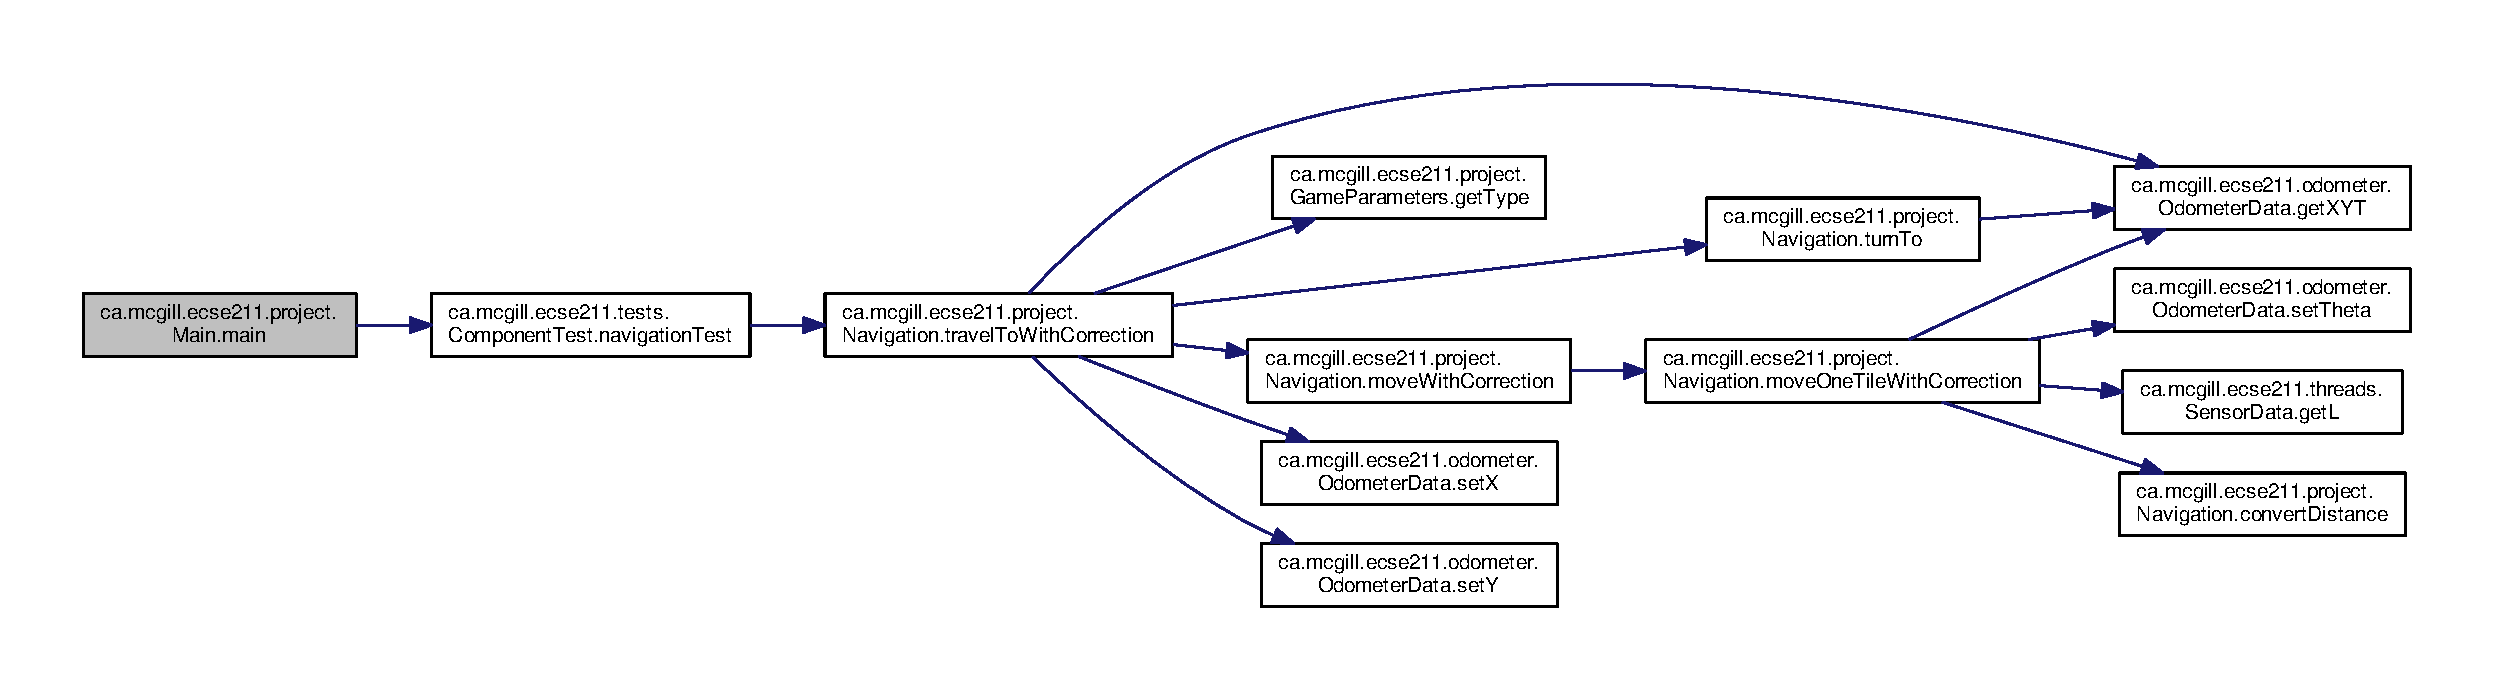
\includegraphics[width=350pt]{classca_1_1mcgill_1_1ecse211_1_1project_1_1_main_af681b5dc675c13ed284071cc135f5fd3_cgraph}
\end{center}
\end{figure}


\subsection{Member Data Documentation}
\mbox{\Hypertarget{classca_1_1mcgill_1_1ecse211_1_1project_1_1_main_af6f7b8fffddcf855f74fe128d2e23ea1}\label{classca_1_1mcgill_1_1ecse211_1_1project_1_1_main_af6f7b8fffddcf855f74fe128d2e23ea1}} 
\index{ca\+::mcgill\+::ecse211\+::project\+::\+Main@{ca\+::mcgill\+::ecse211\+::project\+::\+Main}!test@{test}}
\index{test@{test}!ca\+::mcgill\+::ecse211\+::project\+::\+Main@{ca\+::mcgill\+::ecse211\+::project\+::\+Main}}
\subsubsection{\texorpdfstring{test}{test}}
{\footnotesize\ttfamily boolean ca.\+mcgill.\+ecse211.\+project.\+Main.\+test = false\hspace{0.3cm}{\ttfamily [static]}}

This variable decides whether or not to enable our tests 

Definition at line 21 of file Main.\+java.



The documentation for this class was generated from the following file\+:\begin{DoxyCompactItemize}
\item 
/home/ccc/\+Final\+Project/src/ca/mcgill/ecse211/project/\hyperlink{_main_8java}{Main.\+java}\end{DoxyCompactItemize}

\hypertarget{classca_1_1mcgill_1_1ecse211_1_1project_1_1_navigation}{}\section{ca.\+mcgill.\+ecse211.\+project.\+Navigation Class Reference}
\label{classca_1_1mcgill_1_1ecse211_1_1project_1_1_navigation}\index{ca.\+mcgill.\+ecse211.\+project.\+Navigation@{ca.\+mcgill.\+ecse211.\+project.\+Navigation}}
\subsection*{Public Member Functions}
\begin{DoxyCompactItemize}
\item 
\hyperlink{classca_1_1mcgill_1_1ecse211_1_1project_1_1_navigation_aaee14b67c392ddd951e3ce21224c3e56}{Navigation} (E\+V3\+Large\+Regulated\+Motor left\+Motor, E\+V3\+Large\+Regulated\+Motor right\+Motor)  throws Odometer\+Exceptions 
\item 
void \hyperlink{classca_1_1mcgill_1_1ecse211_1_1project_1_1_navigation_ab01db7b8a871acd45e7dd16922abc15e}{set\+Slow\+Acc} ()
\item 
double \hyperlink{classca_1_1mcgill_1_1ecse211_1_1project_1_1_navigation_a4376e54162df8f123ca3b52e4fd2f38d}{calculate\+Angle\+To} (double x, double y)
\item 
void \hyperlink{classca_1_1mcgill_1_1ecse211_1_1project_1_1_navigation_a3d8354490a2d8c36090d794c25d33421}{travel\+To} (double x, double y, int speed)
\item 
void \hyperlink{classca_1_1mcgill_1_1ecse211_1_1project_1_1_navigation_ae7230e905494002087416294f12cae6a}{travel\+To\+With\+Correction} (int x, int y, boolean avoid)
\item 
synchronized void \hyperlink{classca_1_1mcgill_1_1ecse211_1_1project_1_1_navigation_a48eeb9ae2da23664421e8da5642054c7}{move\+With\+Correction} (double distance, double theta)
\item 
void \hyperlink{classca_1_1mcgill_1_1ecse211_1_1project_1_1_navigation_afbe677941e2bd44e35452e1eff508ae9}{move\+One\+Tile\+With\+Correction} (double theta)
\item 
synchronized void \hyperlink{classca_1_1mcgill_1_1ecse211_1_1project_1_1_navigation_a3bbe0645f2b3b3d0986b4a707fb5a00c}{turn\+To} (double angle)
\item 
void \hyperlink{classca_1_1mcgill_1_1ecse211_1_1project_1_1_navigation_a4b52e605d3ea2f9bcd9481ae2c69ba39}{go\+Through\+Tunnel} ()  throws Exception 
\item 
void \hyperlink{classca_1_1mcgill_1_1ecse211_1_1project_1_1_navigation_a1a808e665b8dd5b8e79b0580724d239c}{search\+Ring\+Set} (\hyperlink{classca_1_1mcgill_1_1ecse211_1_1project_1_1_ring_searcher}{Ring\+Searcher} searcher, boolean correct, boolean reset)
\item 
void \hyperlink{classca_1_1mcgill_1_1ecse211_1_1project_1_1_navigation_ad74286ad36d333bfaf57661837457b76}{turn} (int angle)
\item 
void \hyperlink{classca_1_1mcgill_1_1ecse211_1_1project_1_1_navigation_a7c66610c5b7496ddb35d342ab2cd3f08}{forward} (int speed, double distance)
\item 
void \hyperlink{classca_1_1mcgill_1_1ecse211_1_1project_1_1_navigation_ae8530d181ffd790ff9dea5eeab54b1a1}{stop} ()
\end{DoxyCompactItemize}
\subsection*{Static Public Member Functions}
\begin{DoxyCompactItemize}
\item 
static int \hyperlink{classca_1_1mcgill_1_1ecse211_1_1project_1_1_navigation_ac9e260bcd619ffa4820d7d0de7ea1c12}{convert\+Distance} (double radius, double distance)
\end{DoxyCompactItemize}


\subsection{Detailed Description}
The Navigator class extends the functionality of the \hyperlink{classca_1_1mcgill_1_1ecse211_1_1project_1_1_navigation}{Navigation} class. It offers an alternative \hyperlink{classca_1_1mcgill_1_1ecse211_1_1project_1_1_navigation_a3d8354490a2d8c36090d794c25d33421}{travel\+To()} method which uses a state machine to implement obstacle avoidance.

The Navigator class does not override any of the methods in \hyperlink{classca_1_1mcgill_1_1ecse211_1_1project_1_1_navigation}{Navigation}. All methods with the same name are overloaded i.\+e. the Navigator version takes different parameters than the \hyperlink{classca_1_1mcgill_1_1ecse211_1_1project_1_1_navigation}{Navigation} version.

This is useful if, for instance, you want to force travel without obstacle detection over small distances. One place where you might want to do this is in the Obstacle\+Avoidance class. Another place is methods that implement specific features for future milestones such as retrieving an object.

\begin{DoxyAuthor}{Author}
Caspar Cedro 

Percy Chen 

Patrick Erath 

Anssam Ghezala 

Susan Matuszewski 

Kamy Moussavi Kafi 
\end{DoxyAuthor}


Definition at line 30 of file Navigation.\+java.



\subsection{Constructor \& Destructor Documentation}
\mbox{\Hypertarget{classca_1_1mcgill_1_1ecse211_1_1project_1_1_navigation_aaee14b67c392ddd951e3ce21224c3e56}\label{classca_1_1mcgill_1_1ecse211_1_1project_1_1_navigation_aaee14b67c392ddd951e3ce21224c3e56}} 
\index{ca\+::mcgill\+::ecse211\+::project\+::\+Navigation@{ca\+::mcgill\+::ecse211\+::project\+::\+Navigation}!Navigation@{Navigation}}
\index{Navigation@{Navigation}!ca\+::mcgill\+::ecse211\+::project\+::\+Navigation@{ca\+::mcgill\+::ecse211\+::project\+::\+Navigation}}
\subsubsection{\texorpdfstring{Navigation()}{Navigation()}}
{\footnotesize\ttfamily ca.\+mcgill.\+ecse211.\+project.\+Navigation.\+Navigation (\begin{DoxyParamCaption}\item[{E\+V3\+Large\+Regulated\+Motor}]{left\+Motor,  }\item[{E\+V3\+Large\+Regulated\+Motor}]{right\+Motor }\end{DoxyParamCaption}) throws \hyperlink{classca_1_1mcgill_1_1ecse211_1_1odometer_1_1_odometer_exceptions}{Odometer\+Exceptions}}

This navigation class constructor sets up our robot to begin navigating a particular map


\begin{DoxyParams}{Parameters}
{\em left\+Motor} & The E\+V3\+Large\+Regulated\+Motor instance for our left motor \\
\hline
{\em right\+Motor} & The E\+V3\+Large\+Regulated\+Motor instance for our right motor \\
\hline
\end{DoxyParams}


Definition at line 61 of file Navigation.\+java.


\begin{DoxyCode}
62                                 \{
63     this.odometer = Odometer.\hyperlink{classca_1_1mcgill_1_1ecse211_1_1odometer_1_1_odometer_a99171f11e34dea918fa9dd069d721439}{getOdometer}();
64     this.leftMotor = leftMotor;
65     this.rightMotor = rightMotor;
66     this.data = SensorData.\hyperlink{classca_1_1mcgill_1_1ecse211_1_1threads_1_1_sensor_data_a8260aba53b4474ca1275e4ce26157977}{getSensorData}();
67     \textcolor{keywordflow}{for} (EV3LargeRegulatedMotor motor : \textcolor{keyword}{new} EV3LargeRegulatedMotor[] \{this.leftMotor,
68         this.rightMotor\}) \{
69       motor.stop();
70       motor.setAcceleration(Q\_ACCELERATION);
71     \}
72   \}
\end{DoxyCode}
Here is the call graph for this function\+:\nopagebreak
\begin{figure}[H]
\begin{center}
\leavevmode
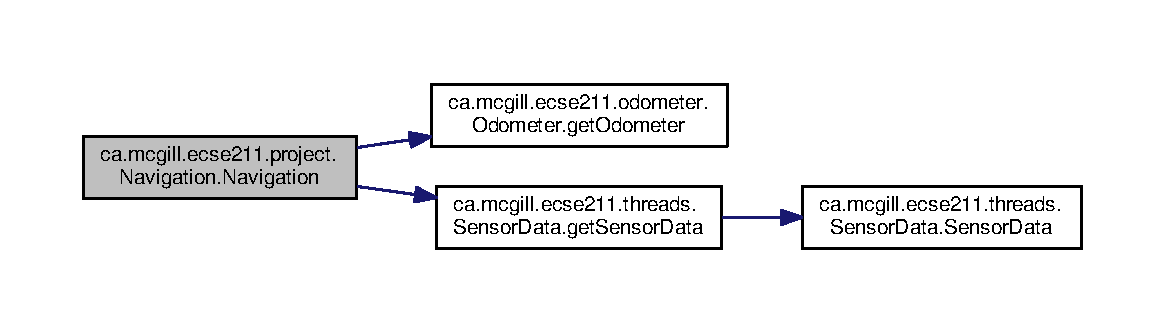
\includegraphics[width=350pt]{classca_1_1mcgill_1_1ecse211_1_1project_1_1_navigation_aaee14b67c392ddd951e3ce21224c3e56_cgraph}
\end{center}
\end{figure}


\subsection{Member Function Documentation}
\mbox{\Hypertarget{classca_1_1mcgill_1_1ecse211_1_1project_1_1_navigation_a4376e54162df8f123ca3b52e4fd2f38d}\label{classca_1_1mcgill_1_1ecse211_1_1project_1_1_navigation_a4376e54162df8f123ca3b52e4fd2f38d}} 
\index{ca\+::mcgill\+::ecse211\+::project\+::\+Navigation@{ca\+::mcgill\+::ecse211\+::project\+::\+Navigation}!calculate\+Angle\+To@{calculate\+Angle\+To}}
\index{calculate\+Angle\+To@{calculate\+Angle\+To}!ca\+::mcgill\+::ecse211\+::project\+::\+Navigation@{ca\+::mcgill\+::ecse211\+::project\+::\+Navigation}}
\subsubsection{\texorpdfstring{calculate\+Angle\+To()}{calculateAngleTo()}}
{\footnotesize\ttfamily double ca.\+mcgill.\+ecse211.\+project.\+Navigation.\+calculate\+Angle\+To (\begin{DoxyParamCaption}\item[{double}]{x,  }\item[{double}]{y }\end{DoxyParamCaption})}

This method calculate the angle for the robot to rotate facing certain point


\begin{DoxyParams}{Parameters}
{\em x} & x coordinate of the point \\
\hline
{\em y} & y coordinate of the point \\
\hline
\end{DoxyParams}
\begin{DoxyReturn}{Returns}
\+: rotation needed in degree 
\end{DoxyReturn}


Definition at line 85 of file Navigation.\+java.


\begin{DoxyCode}
85                                                      \{
86     \textcolor{keywordtype}{double} dX = x - odometer.\hyperlink{classca_1_1mcgill_1_1ecse211_1_1odometer_1_1_odometer_data_a8f40f0264c68f0cbed4fff1723ae7863}{getXYT}()[0];
87     \textcolor{keywordtype}{double} dY = y - odometer.\hyperlink{classca_1_1mcgill_1_1ecse211_1_1odometer_1_1_odometer_data_a8f40f0264c68f0cbed4fff1723ae7863}{getXYT}()[1];
88     \textcolor{keywordtype}{double} theta = Math.atan(dX / dY);
89     \textcolor{keywordflow}{if} (dY < 0 && theta < Math.PI)
90       theta += Math.PI;
91     \textcolor{keywordflow}{return} theta;
92   \}
\end{DoxyCode}
Here is the call graph for this function\+:\nopagebreak
\begin{figure}[H]
\begin{center}
\leavevmode
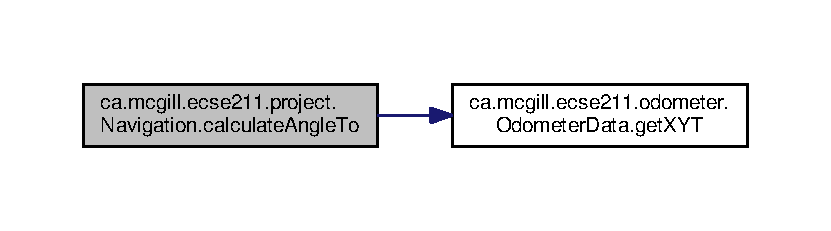
\includegraphics[width=350pt]{classca_1_1mcgill_1_1ecse211_1_1project_1_1_navigation_a4376e54162df8f123ca3b52e4fd2f38d_cgraph}
\end{center}
\end{figure}
Here is the caller graph for this function\+:
\nopagebreak
\begin{figure}[H]
\begin{center}
\leavevmode
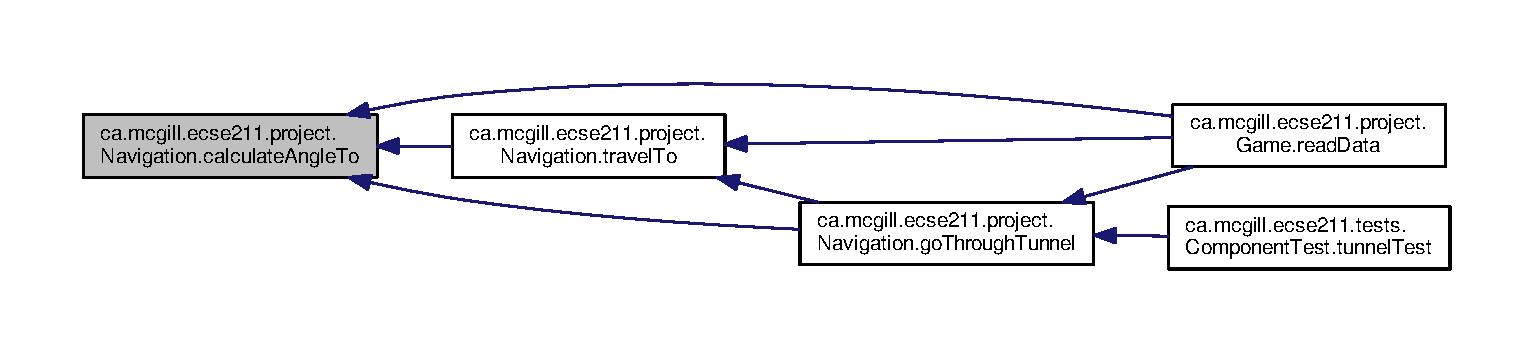
\includegraphics[width=350pt]{classca_1_1mcgill_1_1ecse211_1_1project_1_1_navigation_a4376e54162df8f123ca3b52e4fd2f38d_icgraph}
\end{center}
\end{figure}
\mbox{\Hypertarget{classca_1_1mcgill_1_1ecse211_1_1project_1_1_navigation_ac9e260bcd619ffa4820d7d0de7ea1c12}\label{classca_1_1mcgill_1_1ecse211_1_1project_1_1_navigation_ac9e260bcd619ffa4820d7d0de7ea1c12}} 
\index{ca\+::mcgill\+::ecse211\+::project\+::\+Navigation@{ca\+::mcgill\+::ecse211\+::project\+::\+Navigation}!convert\+Distance@{convert\+Distance}}
\index{convert\+Distance@{convert\+Distance}!ca\+::mcgill\+::ecse211\+::project\+::\+Navigation@{ca\+::mcgill\+::ecse211\+::project\+::\+Navigation}}
\subsubsection{\texorpdfstring{convert\+Distance()}{convertDistance()}}
{\footnotesize\ttfamily static int ca.\+mcgill.\+ecse211.\+project.\+Navigation.\+convert\+Distance (\begin{DoxyParamCaption}\item[{double}]{radius,  }\item[{double}]{distance }\end{DoxyParamCaption})\hspace{0.3cm}{\ttfamily [static]}}

This method allows the conversion of a distance to the total rotation of each wheel need to cover that distance.


\begin{DoxyParams}{Parameters}
{\em radius} & The radius of our wheels \\
\hline
{\em distance} & The distance traveled \\
\hline
\end{DoxyParams}
\begin{DoxyReturn}{Returns}
A converted distance 
\end{DoxyReturn}


Definition at line 658 of file Navigation.\+java.


\begin{DoxyCode}
658                                                                     \{
659     \textcolor{keywordflow}{return} (\textcolor{keywordtype}{int}) ((180.0 * distance) / (Math.PI * radius));
660   \}
\end{DoxyCode}
Here is the caller graph for this function\+:
\nopagebreak
\begin{figure}[H]
\begin{center}
\leavevmode
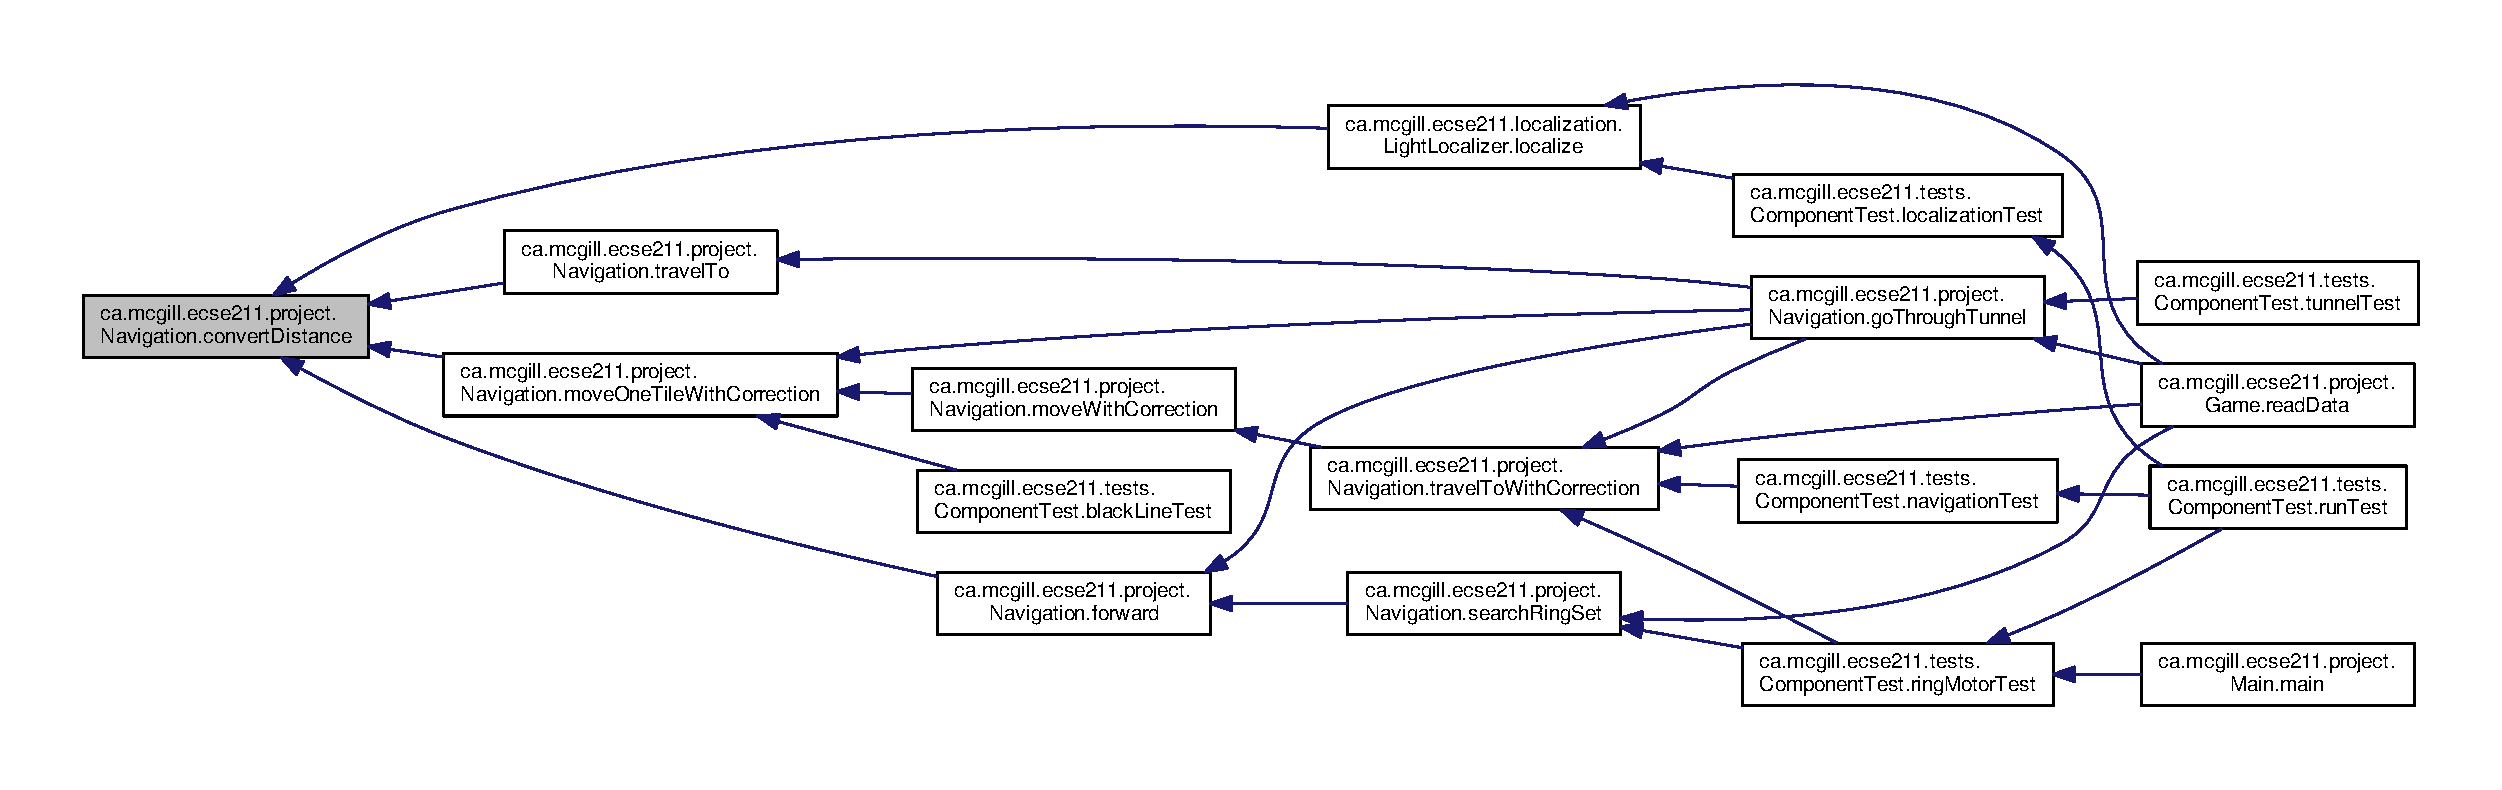
\includegraphics[width=350pt]{classca_1_1mcgill_1_1ecse211_1_1project_1_1_navigation_ac9e260bcd619ffa4820d7d0de7ea1c12_icgraph}
\end{center}
\end{figure}
\mbox{\Hypertarget{classca_1_1mcgill_1_1ecse211_1_1project_1_1_navigation_a7c66610c5b7496ddb35d342ab2cd3f08}\label{classca_1_1mcgill_1_1ecse211_1_1project_1_1_navigation_a7c66610c5b7496ddb35d342ab2cd3f08}} 
\index{ca\+::mcgill\+::ecse211\+::project\+::\+Navigation@{ca\+::mcgill\+::ecse211\+::project\+::\+Navigation}!forward@{forward}}
\index{forward@{forward}!ca\+::mcgill\+::ecse211\+::project\+::\+Navigation@{ca\+::mcgill\+::ecse211\+::project\+::\+Navigation}}
\subsubsection{\texorpdfstring{forward()}{forward()}}
{\footnotesize\ttfamily void ca.\+mcgill.\+ecse211.\+project.\+Navigation.\+forward (\begin{DoxyParamCaption}\item[{int}]{speed,  }\item[{double}]{distance }\end{DoxyParamCaption})}

Move the robot forward


\begin{DoxyParams}{Parameters}
{\em speed} & speed to be taken \\
\hline
{\em distance} & distacne to travel \\
\hline
\end{DoxyParams}


Definition at line 629 of file Navigation.\+java.


\begin{DoxyCode}
629                                                   \{
630     leftMotor.setSpeed(speed);
631     rightMotor.setSpeed(speed);
632     \textcolor{keywordflow}{try} \{
633       Thread.sleep(100);
634     \} \textcolor{keywordflow}{catch} (InterruptedException e) \{
635       \textcolor{comment}{// TODO Auto-generated catch block}
636       e.printStackTrace();
637     \}
638     leftMotor.rotate(\hyperlink{classca_1_1mcgill_1_1ecse211_1_1project_1_1_navigation_ac9e260bcd619ffa4820d7d0de7ea1c12}{convertDistance}(Game.WHEEL\_RAD, distance * Game.TILE), \textcolor{keyword}{true});
639     rightMotor.rotate(\hyperlink{classca_1_1mcgill_1_1ecse211_1_1project_1_1_navigation_ac9e260bcd619ffa4820d7d0de7ea1c12}{convertDistance}(Game.WHEEL\_RAD, distance * Game.TILE), \textcolor{keyword}{false});
640   \}
\end{DoxyCode}
Here is the call graph for this function\+:
\nopagebreak
\begin{figure}[H]
\begin{center}
\leavevmode
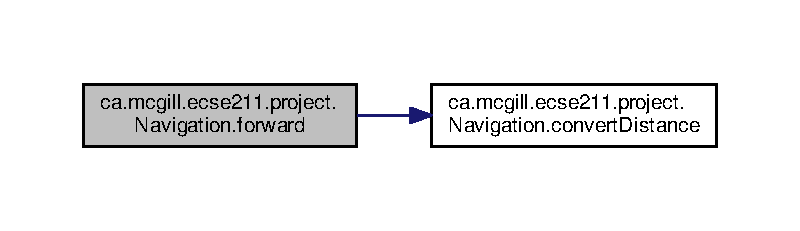
\includegraphics[width=350pt]{classca_1_1mcgill_1_1ecse211_1_1project_1_1_navigation_a7c66610c5b7496ddb35d342ab2cd3f08_cgraph}
\end{center}
\end{figure}
Here is the caller graph for this function\+:
\nopagebreak
\begin{figure}[H]
\begin{center}
\leavevmode
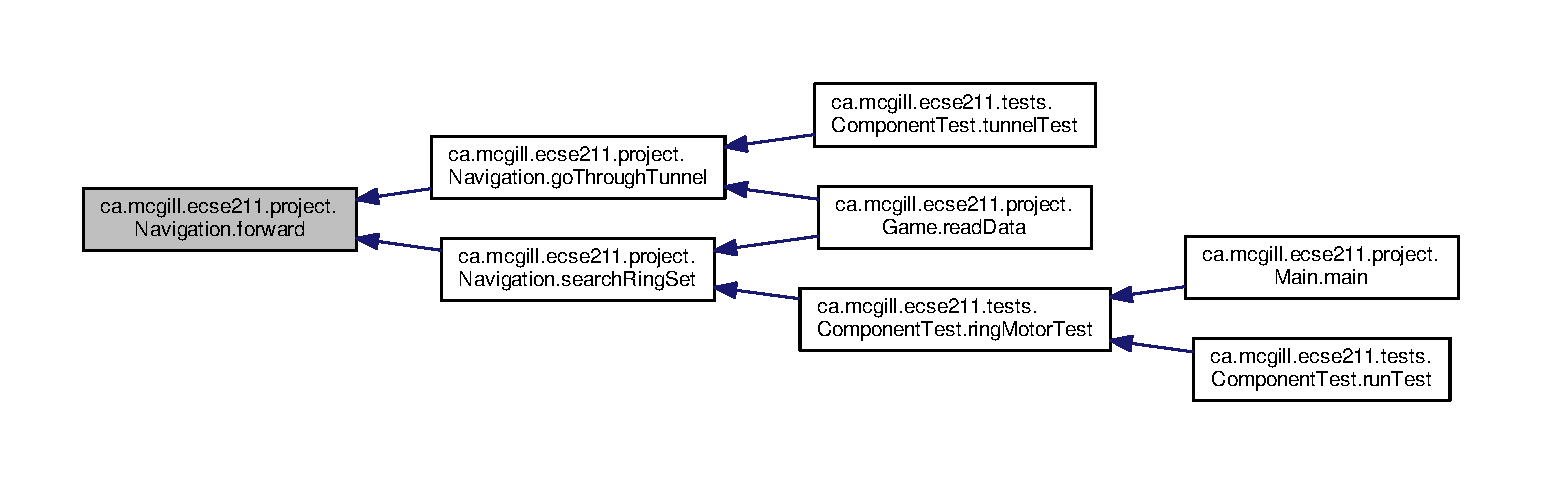
\includegraphics[width=350pt]{classca_1_1mcgill_1_1ecse211_1_1project_1_1_navigation_a7c66610c5b7496ddb35d342ab2cd3f08_icgraph}
\end{center}
\end{figure}
\mbox{\Hypertarget{classca_1_1mcgill_1_1ecse211_1_1project_1_1_navigation_a4b52e605d3ea2f9bcd9481ae2c69ba39}\label{classca_1_1mcgill_1_1ecse211_1_1project_1_1_navigation_a4b52e605d3ea2f9bcd9481ae2c69ba39}} 
\index{ca\+::mcgill\+::ecse211\+::project\+::\+Navigation@{ca\+::mcgill\+::ecse211\+::project\+::\+Navigation}!go\+Through\+Tunnel@{go\+Through\+Tunnel}}
\index{go\+Through\+Tunnel@{go\+Through\+Tunnel}!ca\+::mcgill\+::ecse211\+::project\+::\+Navigation@{ca\+::mcgill\+::ecse211\+::project\+::\+Navigation}}
\subsubsection{\texorpdfstring{go\+Through\+Tunnel()}{goThroughTunnel()}}
{\footnotesize\ttfamily void ca.\+mcgill.\+ecse211.\+project.\+Navigation.\+go\+Through\+Tunnel (\begin{DoxyParamCaption}{ }\end{DoxyParamCaption}) throws Exception}

found the tunnel based on the ll and ur coordinate, after the method, the robot will go the the entrance of the tunnel facing the tunnel it returns the distance it needs to go for \mbox{[}x\mbox{]} and \mbox{[}y\mbox{]} in order to go through the tunnel


\begin{DoxyExceptions}{Exceptions}
{\em Exception} & \\
\hline
\end{DoxyExceptions}


Definition at line 397 of file Navigation.\+java.


\begin{DoxyCode}
397                                                  \{
398     \textcolor{keywordtype}{int} distance = 0;
399     \textcolor{keywordtype}{int}[] ll, ur;
400     \textcolor{comment}{// first use ll and ur coordinate to calculate lr and ul of the tunnel}
401     ll = GameParameters.TN\_LL;
402     ur = GameParameters.TN\_UR;
403     \textcolor{keywordtype}{int}[] lr = \{ll[0], ur[1]\};
404     \textcolor{keywordtype}{int}[] ul = \{ur[0], ll[1]\};
405 
406     \textcolor{comment}{// clone the four points (to make sure we are not modifying the original one)}
407     \textcolor{keywordtype}{int}[][] corners = \{ll.clone(), lr.clone(), ul.clone(), ur.clone()\};
408     ArrayList<int[]> notIn = \textcolor{keyword}{new} ArrayList<int[]>();
409     ArrayList<int[]> points = \textcolor{keyword}{new} ArrayList<int[]>();
410     \textcolor{keywordtype}{double}[] position = odometer.\hyperlink{classca_1_1mcgill_1_1ecse211_1_1odometer_1_1_odometer_data_a8f40f0264c68f0cbed4fff1723ae7863}{getXYT}();
411 
412     \textcolor{comment}{// search for the points that are the same as the current area of the robot}
413     \textcolor{comment}{// these are the entrance of the tunnel, also find the other two points, those}
414     \textcolor{comment}{// are the exit of the tunnel}
415     GameParameters.AreaType type =
416         GameParameters.getType((\textcolor{keywordtype}{int}) Math.round(position[0]), (int) Math.round(position[1]));
417     \textcolor{keywordflow}{for} (\textcolor{keywordtype}{int}[] point : corners) \{
418       \textcolor{keywordflow}{if} (GameParameters.getType(point[0], point[1]) == type) \{
419         points.add(point);
420       \} \textcolor{keywordflow}{else} \{
421         notIn.add(point);
422       \}
423     \}
424 
425     \textcolor{comment}{// Sort the two point at exit by the distance to the destination}
426     \textcolor{keywordflow}{if} (type == GameParameters.AreaType.InStarting) \{
427       Collections.sort(notIn, \textcolor{keyword}{new} GameUtil.RingSetComparator());
428     \} \textcolor{keywordflow}{else} \textcolor{keywordflow}{if} (type == GameParameters.AreaType.Searching) \{
429       Collections.sort(notIn, \textcolor{keyword}{new} GameUtil.StartingComparator());
430     \}
431 
432     \textcolor{comment}{// find the direction and length of the tunnel}
433     \textcolor{comment}{// we know the entrance two points of the tunnel, so this means}
434     \textcolor{comment}{// the two points must have either x or y coordinate identical.}
435     \textcolor{comment}{// that's the direction of the tunnel as well}
436     \textcolor{comment}{// after identify it's direction, we find whether it is positive}
437     \textcolor{comment}{// or negative directed}
438     \textcolor{keywordflow}{if} (points.get(0)[0] == points.get(1)[0]) \{
439       distance = Math.abs(notIn.get(0)[0] - points.get(0)[0]);
440       \textcolor{keywordtype}{int} multi = notIn.get(0)[0] - points.get(0)[0] < 0 ? 1 : -1;
441       travelToTunnelEntrance(points, 0, multi);
442       \textcolor{keywordflow}{for} (\textcolor{keywordtype}{int} i = 0; i < notIn.size(); i++) \{
443         \textcolor{comment}{// this step is to find the nearest two points that we can go two}
444         \textcolor{comment}{// after exit the tunnel}
445         notIn.get(i)[0] = notIn.get(i)[0] - multi * 1;
446       \}
447     \} \textcolor{keywordflow}{else} \{
448       distance = Math.abs(notIn.get(0)[1] - points.get(0)[1]);
449       \textcolor{keywordtype}{int} multi = notIn.get(0)[1] - points.get(0)[1] < 0 ? 1 : -1;
450       travelToTunnelEntrance(points, 1, multi);
451       \textcolor{keywordflow}{for} (\textcolor{keywordtype}{int} i = 0; i < notIn.size(); i++) \{
452         \textcolor{comment}{// this step is to find the nearest two points that we can go two}
453         \textcolor{comment}{// after exit the tunnel}
454         notIn.get(i)[1] = notIn.get(i)[1] - multi * 1;
455       \}
456     \}
457 
458     \textcolor{keywordtype}{double}[] tunnelEnd = GameUtil.average(notIn.get(0), notIn.get(1));
459     \textcolor{keywordtype}{double} angleThoughTunnel = Math.toDegrees(\hyperlink{classca_1_1mcgill_1_1ecse211_1_1project_1_1_navigation_a4376e54162df8f123ca3b52e4fd2f38d}{calculateAngleTo}(tunnelEnd[0], tunnelEnd[1]))
      ;
460     \hyperlink{classca_1_1mcgill_1_1ecse211_1_1project_1_1_navigation_a3bbe0645f2b3b3d0986b4a707fb5a00c}{turnTo}(angleThoughTunnel);
461 
462     \textcolor{comment}{// goback To correct}
463       moveBackWithCorrection();
464 
465     \textcolor{comment}{// turn left -5 to correct the effect of the weight}
466     \hyperlink{classca_1_1mcgill_1_1ecse211_1_1project_1_1_navigation_a7c66610c5b7496ddb35d342ab2cd3f08}{forward}(TUNNEL\_SPEED, 0.5);
467     \hyperlink{classca_1_1mcgill_1_1ecse211_1_1project_1_1_navigation_ad74286ad36d333bfaf57661837457b76}{turn}(TUNNEL\_CORRECTION);
468     \textcolor{keywordflow}{if} (distance == 1) \{
469       \hyperlink{classca_1_1mcgill_1_1ecse211_1_1project_1_1_navigation_a7c66610c5b7496ddb35d342ab2cd3f08}{forward}(TUNNEL\_SPEED, distance + 1 );
470     \} \textcolor{keywordflow}{else} \{
471 
472       \hyperlink{classca_1_1mcgill_1_1ecse211_1_1project_1_1_navigation_a7c66610c5b7496ddb35d342ab2cd3f08}{forward}(TUNNEL\_SPEED, distance + 1 );
473     \}
474 
475     odometer.\hyperlink{classca_1_1mcgill_1_1ecse211_1_1odometer_1_1_odometer_data_a419b8f07c2c5374411c8e62298e9a402}{setTheta}(angleThoughTunnel);
476     \textcolor{comment}{// leftMotor.setAcceleration(N\_ACCELERATION);}
477     \textcolor{comment}{// rightMotor.setAcceleration(N\_ACCELERATION);}
478     \textcolor{comment}{// // rotate additional sensor distances to make sure the sensor will not on the balck line}
479     \textcolor{comment}{// leftMotor.rotate(convertDistance(Game.WHEEL\_RAD, 2*Game.SEN\_DIS), true);}
480     \textcolor{comment}{// rightMotor.rotate(convertDistance(Game.WHEEL\_RAD, 2*Game.SEN\_DIS), false);}
481     this.\hyperlink{classca_1_1mcgill_1_1ecse211_1_1project_1_1_navigation_afbe677941e2bd44e35452e1eff508ae9}{moveOneTileWithCorrection}(angleThoughTunnel);
482     \textcolor{keywordtype}{double}[] after = GameUtil.average(notIn.get(0), notIn.get(1));
483     odometer.\hyperlink{classca_1_1mcgill_1_1ecse211_1_1odometer_1_1_odometer_data_a2911d7215e47f3064defe016b46bfeef}{setX}(after[0]);
484     odometer.\hyperlink{classca_1_1mcgill_1_1ecse211_1_1odometer_1_1_odometer_data_a82986438cd462e66520bc62bb4bd2b75}{setY}(after[1]);
485     \textcolor{comment}{// go to the nearest safe point near tunnel}
486     \textcolor{keywordflow}{for} (\textcolor{keywordtype}{int}[] p : notIn) \{
487       \textcolor{keywordflow}{if} (GameUtil.isSafe(p)) \{
488         \textcolor{keywordtype}{double} toPointAngle = Math.toDegrees(\hyperlink{classca_1_1mcgill_1_1ecse211_1_1project_1_1_navigation_a4376e54162df8f123ca3b52e4fd2f38d}{calculateAngleTo}(p[0], p[1]));
489         \hyperlink{classca_1_1mcgill_1_1ecse211_1_1project_1_1_navigation_a3bbe0645f2b3b3d0986b4a707fb5a00c}{turnTo}(toPointAngle);
490         this.\hyperlink{classca_1_1mcgill_1_1ecse211_1_1project_1_1_navigation_afbe677941e2bd44e35452e1eff508ae9}{moveOneTileWithCorrection}(toPointAngle);
491         odometer.\hyperlink{classca_1_1mcgill_1_1ecse211_1_1odometer_1_1_odometer_data_a2911d7215e47f3064defe016b46bfeef}{setX}(p[0]);
492         odometer.\hyperlink{classca_1_1mcgill_1_1ecse211_1_1odometer_1_1_odometer_data_a82986438cd462e66520bc62bb4bd2b75}{setY}(p[1]);
493         \textcolor{keywordflow}{break};
494       \}
495     \}
496   \}
\end{DoxyCode}
Here is the call graph for this function\+:
\nopagebreak
\begin{figure}[H]
\begin{center}
\leavevmode
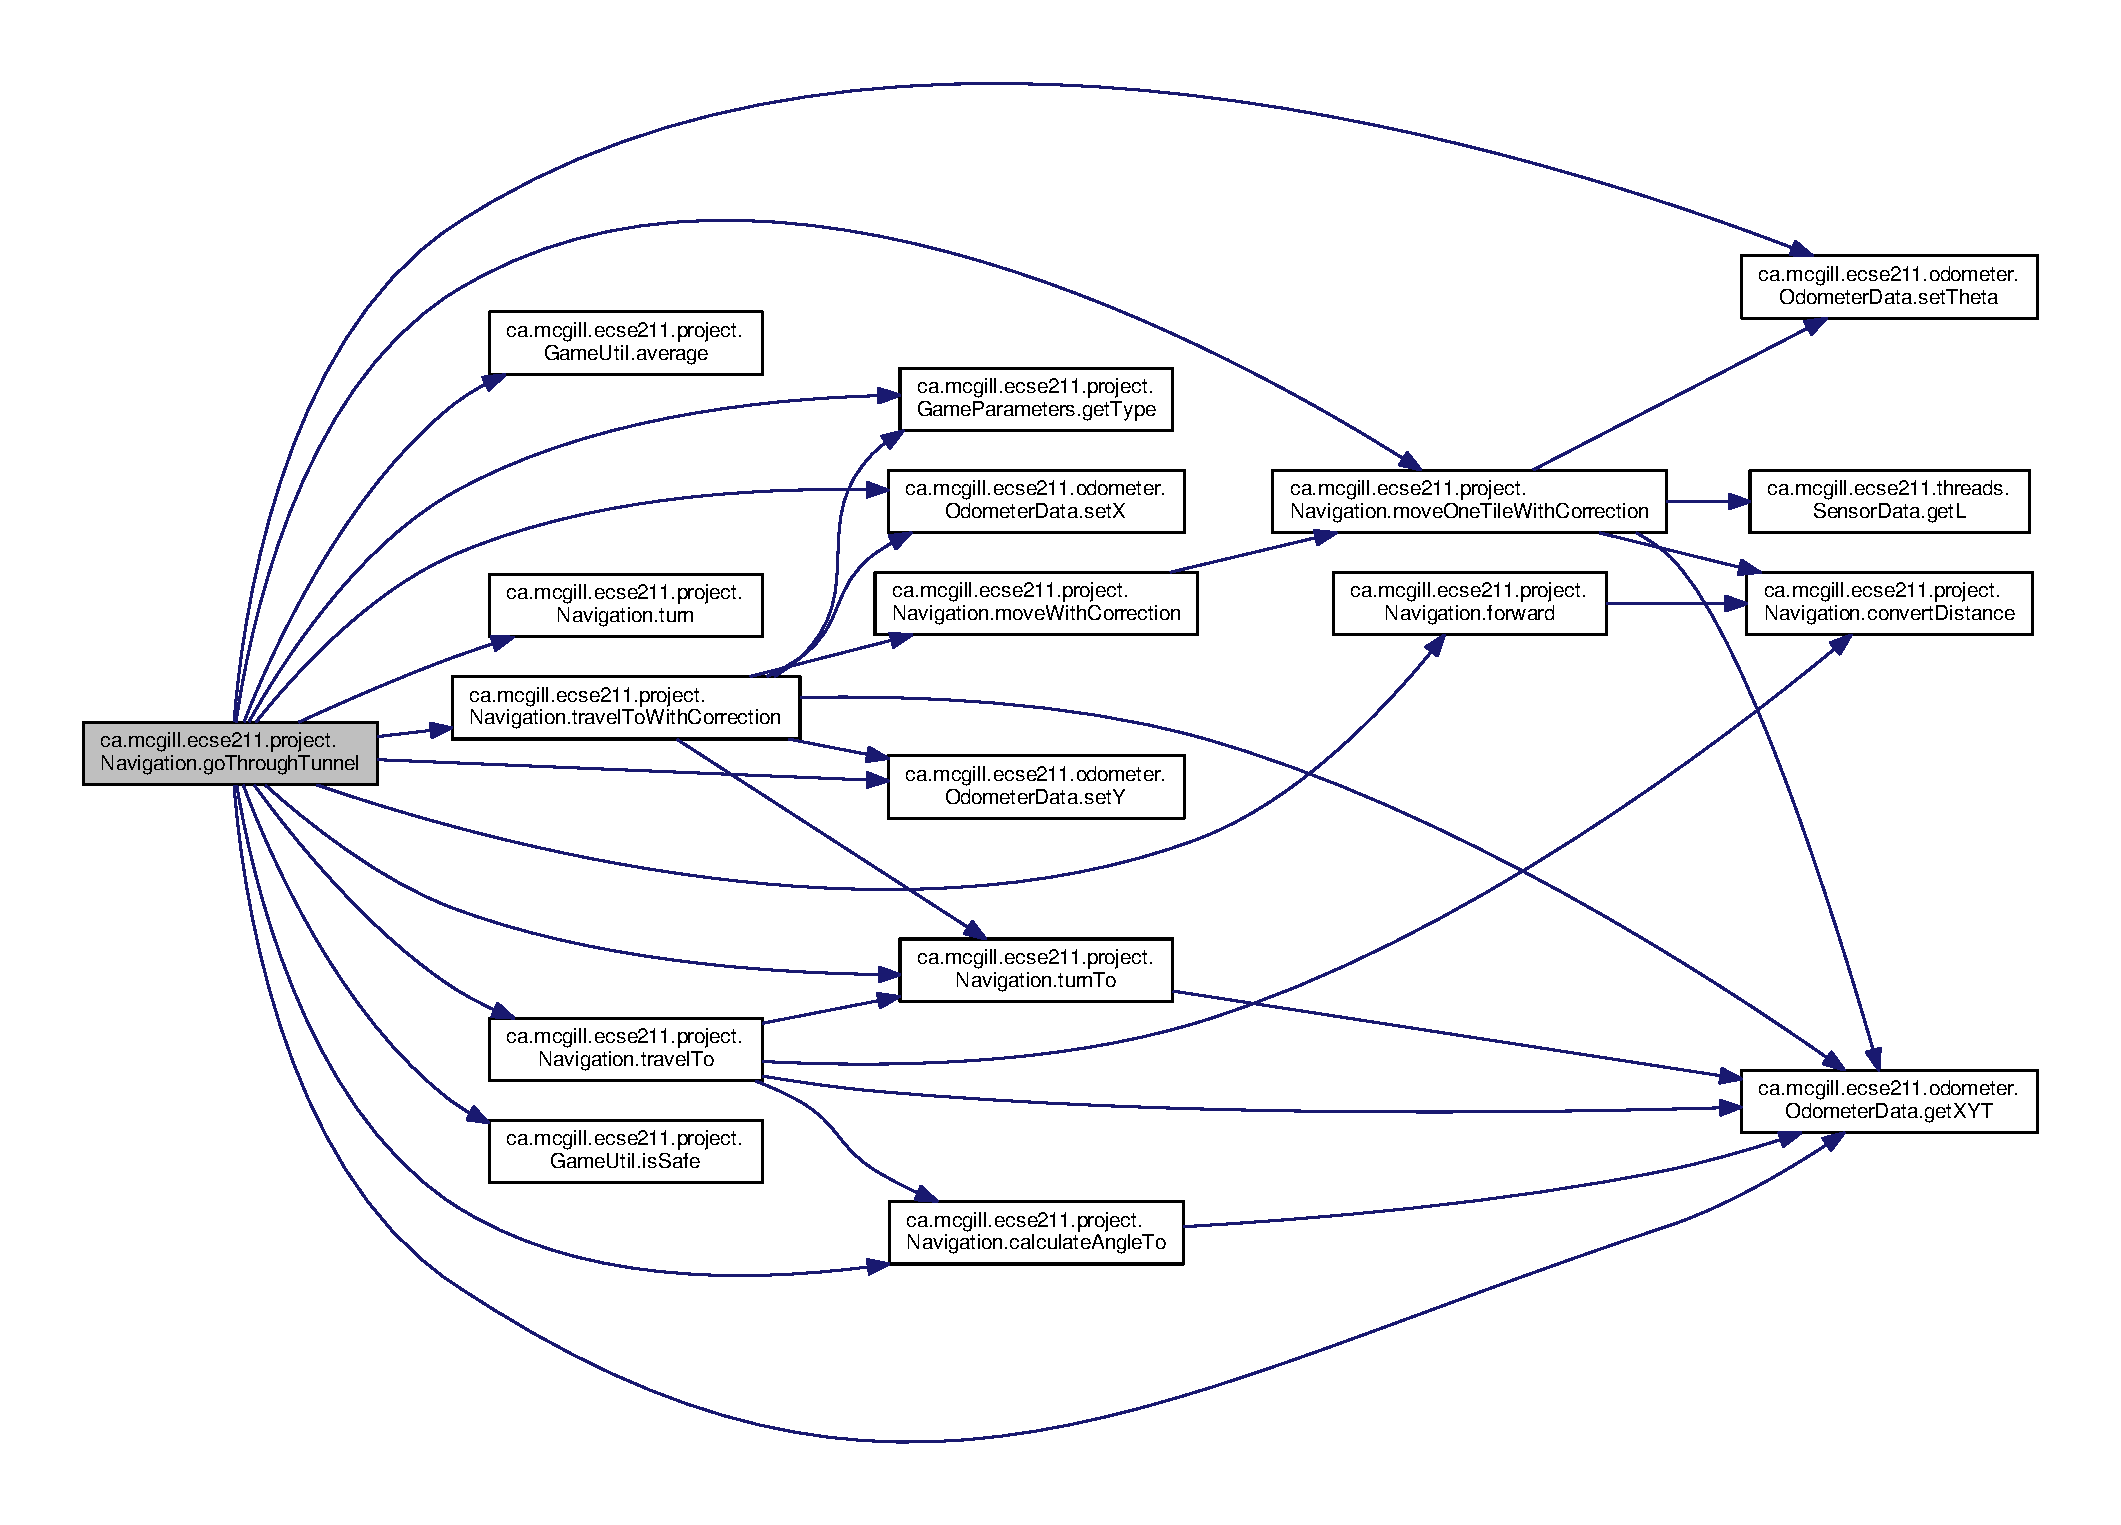
\includegraphics[width=350pt]{classca_1_1mcgill_1_1ecse211_1_1project_1_1_navigation_a4b52e605d3ea2f9bcd9481ae2c69ba39_cgraph}
\end{center}
\end{figure}
Here is the caller graph for this function\+:
\nopagebreak
\begin{figure}[H]
\begin{center}
\leavevmode
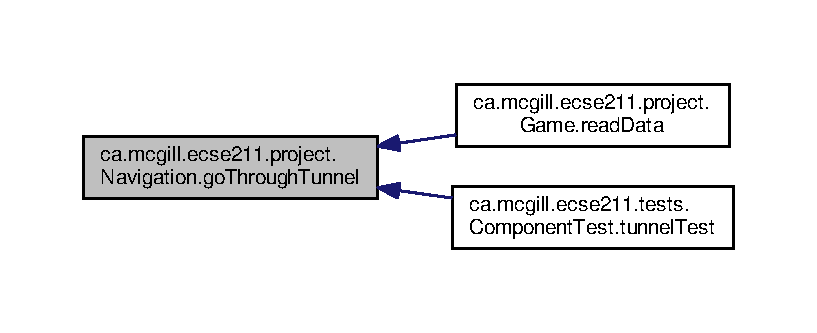
\includegraphics[width=350pt]{classca_1_1mcgill_1_1ecse211_1_1project_1_1_navigation_a4b52e605d3ea2f9bcd9481ae2c69ba39_icgraph}
\end{center}
\end{figure}
\mbox{\Hypertarget{classca_1_1mcgill_1_1ecse211_1_1project_1_1_navigation_afbe677941e2bd44e35452e1eff508ae9}\label{classca_1_1mcgill_1_1ecse211_1_1project_1_1_navigation_afbe677941e2bd44e35452e1eff508ae9}} 
\index{ca\+::mcgill\+::ecse211\+::project\+::\+Navigation@{ca\+::mcgill\+::ecse211\+::project\+::\+Navigation}!move\+One\+Tile\+With\+Correction@{move\+One\+Tile\+With\+Correction}}
\index{move\+One\+Tile\+With\+Correction@{move\+One\+Tile\+With\+Correction}!ca\+::mcgill\+::ecse211\+::project\+::\+Navigation@{ca\+::mcgill\+::ecse211\+::project\+::\+Navigation}}
\subsubsection{\texorpdfstring{move\+One\+Tile\+With\+Correction()}{moveOneTileWithCorrection()}}
{\footnotesize\ttfamily void ca.\+mcgill.\+ecse211.\+project.\+Navigation.\+move\+One\+Tile\+With\+Correction (\begin{DoxyParamCaption}\item[{double}]{theta }\end{DoxyParamCaption})}

This method move the robot one tile until it detect a blackline (ususally one tile)


\begin{DoxyParams}{Parameters}
{\em theta} & \\
\hline
\end{DoxyParams}


Definition at line 257 of file Navigation.\+java.


\begin{DoxyCode}
257                                                       \{
258     \textcolor{comment}{// leftMotor.setAcceleration(N\_ACCELERATION);}
259     \textcolor{comment}{// rightMotor.setAcceleration(N\_ACCELERATION);}
260     leftMotor.setSpeed(FORWARD\_SPEED);
261     rightMotor.setSpeed(FORWARD\_SPEED);
262     leftMotor.forward();
263     rightMotor.forward();
264     moveUntilLineDetection(\textcolor{keyword}{true});
265     odometer.\hyperlink{classca_1_1mcgill_1_1ecse211_1_1odometer_1_1_odometer_data_a419b8f07c2c5374411c8e62298e9a402}{setTheta}(theta);
266   \}
\end{DoxyCode}
Here is the call graph for this function\+:
\nopagebreak
\begin{figure}[H]
\begin{center}
\leavevmode
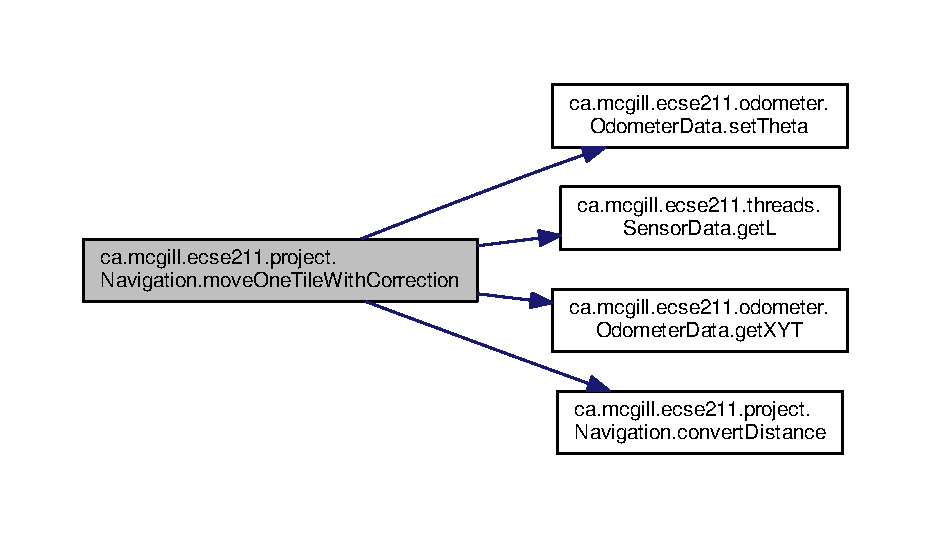
\includegraphics[width=350pt]{classca_1_1mcgill_1_1ecse211_1_1project_1_1_navigation_afbe677941e2bd44e35452e1eff508ae9_cgraph}
\end{center}
\end{figure}
Here is the caller graph for this function\+:
\nopagebreak
\begin{figure}[H]
\begin{center}
\leavevmode
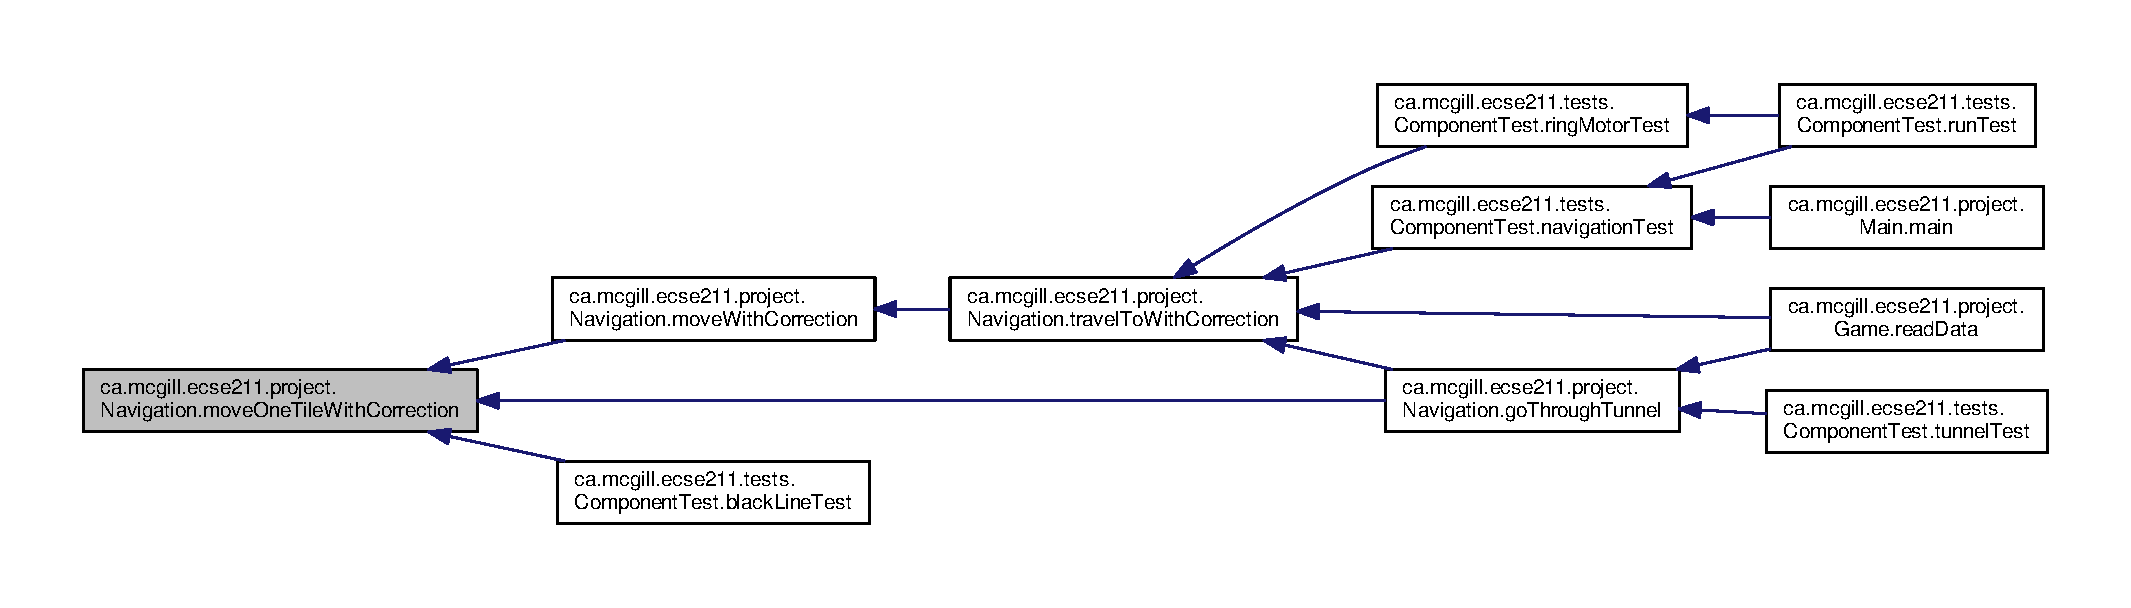
\includegraphics[width=350pt]{classca_1_1mcgill_1_1ecse211_1_1project_1_1_navigation_afbe677941e2bd44e35452e1eff508ae9_icgraph}
\end{center}
\end{figure}
\mbox{\Hypertarget{classca_1_1mcgill_1_1ecse211_1_1project_1_1_navigation_a48eeb9ae2da23664421e8da5642054c7}\label{classca_1_1mcgill_1_1ecse211_1_1project_1_1_navigation_a48eeb9ae2da23664421e8da5642054c7}} 
\index{ca\+::mcgill\+::ecse211\+::project\+::\+Navigation@{ca\+::mcgill\+::ecse211\+::project\+::\+Navigation}!move\+With\+Correction@{move\+With\+Correction}}
\index{move\+With\+Correction@{move\+With\+Correction}!ca\+::mcgill\+::ecse211\+::project\+::\+Navigation@{ca\+::mcgill\+::ecse211\+::project\+::\+Navigation}}
\subsubsection{\texorpdfstring{move\+With\+Correction()}{moveWithCorrection()}}
{\footnotesize\ttfamily synchronized void ca.\+mcgill.\+ecse211.\+project.\+Navigation.\+move\+With\+Correction (\begin{DoxyParamCaption}\item[{double}]{distance,  }\item[{double}]{theta }\end{DoxyParamCaption})}

Move a certain distance with correction along current direction (using coordinate system)


\begin{DoxyParams}{Parameters}
{\em distance} & distance to cover \\
\hline
{\em theta} & theta to be corrected each time \\
\hline
\end{DoxyParams}


Definition at line 228 of file Navigation.\+java.


\begin{DoxyCode}
228                                                                              \{
229     leftMotor.setSpeed(FORWARD\_SPEED);
230     rightMotor.setSpeed(FORWARD\_SPEED);
231 
232     \textcolor{comment}{// correct error of the distance}
233     \textcolor{keywordtype}{int} tiles = Math.abs((\textcolor{keywordtype}{int}) Math.round(distance));
234     \textcolor{keywordflow}{for} (\textcolor{keywordtype}{int} i = 0; i < tiles; i++) \{
235       \hyperlink{classca_1_1mcgill_1_1ecse211_1_1project_1_1_navigation_afbe677941e2bd44e35452e1eff508ae9}{moveOneTileWithCorrection}(theta);
236     \}
237   \}
\end{DoxyCode}
Here is the call graph for this function\+:
\nopagebreak
\begin{figure}[H]
\begin{center}
\leavevmode
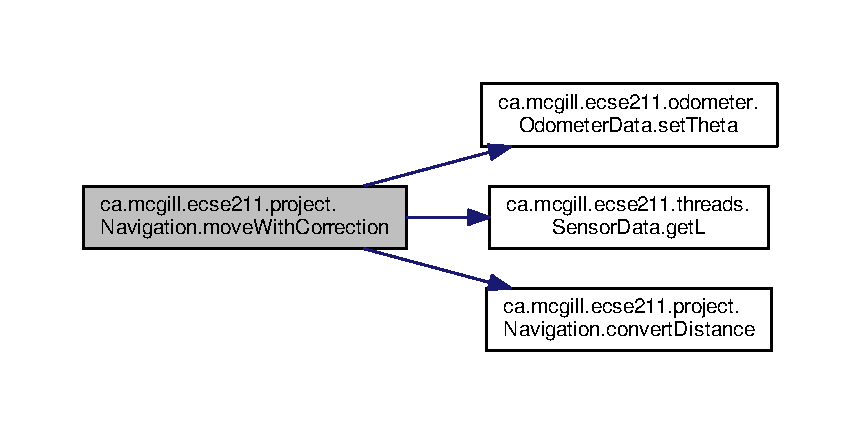
\includegraphics[width=350pt]{classca_1_1mcgill_1_1ecse211_1_1project_1_1_navigation_a48eeb9ae2da23664421e8da5642054c7_cgraph}
\end{center}
\end{figure}
Here is the caller graph for this function\+:
\nopagebreak
\begin{figure}[H]
\begin{center}
\leavevmode
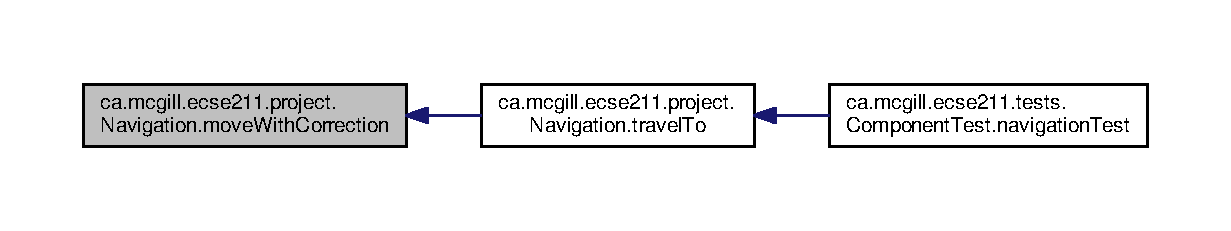
\includegraphics[width=350pt]{classca_1_1mcgill_1_1ecse211_1_1project_1_1_navigation_a48eeb9ae2da23664421e8da5642054c7_icgraph}
\end{center}
\end{figure}
\mbox{\Hypertarget{classca_1_1mcgill_1_1ecse211_1_1project_1_1_navigation_a1a808e665b8dd5b8e79b0580724d239c}\label{classca_1_1mcgill_1_1ecse211_1_1project_1_1_navigation_a1a808e665b8dd5b8e79b0580724d239c}} 
\index{ca\+::mcgill\+::ecse211\+::project\+::\+Navigation@{ca\+::mcgill\+::ecse211\+::project\+::\+Navigation}!search\+Ring\+Set@{search\+Ring\+Set}}
\index{search\+Ring\+Set@{search\+Ring\+Set}!ca\+::mcgill\+::ecse211\+::project\+::\+Navigation@{ca\+::mcgill\+::ecse211\+::project\+::\+Navigation}}
\subsubsection{\texorpdfstring{search\+Ring\+Set()}{searchRingSet()}}
{\footnotesize\ttfamily void ca.\+mcgill.\+ecse211.\+project.\+Navigation.\+search\+Ring\+Set (\begin{DoxyParamCaption}\item[{\hyperlink{classca_1_1mcgill_1_1ecse211_1_1project_1_1_ring_searcher}{Ring\+Searcher}}]{searcher,  }\item[{boolean}]{correct,  }\item[{boolean}]{reset }\end{DoxyParamCaption})}


\begin{DoxyItemize}
\item this method approaches the ring set by paying attention to the reading of us sensor, stops at the place when the robot can reach the ring
\end{DoxyItemize}


\begin{DoxyParams}{Parameters}
{\em searcher} & ring searcher \\
\hline
{\em correct} & whether correct the position when searching ring (cannot do this when at boundary) \\
\hline
{\em reset} & whether reset the rod motor to the original position \\
\hline
\end{DoxyParams}


Definition at line 540 of file Navigation.\+java.


\begin{DoxyCode}
540                                                                                    \{
541     \textcolor{comment}{// Go backward to detect the line and correct the rotation}
542     \textcolor{comment}{// leftMotor.setAcceleration(N\_ACCELERATION);}
543     \textcolor{comment}{// rightMotor.setAcceleration(N\_ACCELERATION);}
544     leftMotor.setSpeed(FORWARD\_SPEED);
545     rightMotor.setSpeed(FORWARD\_SPEED);
546     \textcolor{keywordflow}{try} \{
547       Thread.sleep(100);
548     \} \textcolor{keywordflow}{catch} (InterruptedException e) \{
549       \textcolor{comment}{// TODO Auto-generated catch block}
550       e.printStackTrace();
551     \}
552     \textcolor{keywordtype}{double} theta = odometer.\hyperlink{classca_1_1mcgill_1_1ecse211_1_1odometer_1_1_odometer_data_a8f40f0264c68f0cbed4fff1723ae7863}{getXYT}()[2];
553 
554     \textcolor{comment}{// if we do correction, we need to forward more (for the sensor distance)}
555     \textcolor{keywordflow}{if} (correct) \{
556       leftMotor.backward();
557       rightMotor.backward();
558       moveUntilLineDetection(\textcolor{keyword}{true});
559       \textcolor{comment}{// Forward for 3 cm (approach the ring set)}
560       \textcolor{comment}{//forward(FORWARD\_SPEED, 2.5 / Game.TILE);}
561     \} \textcolor{keywordflow}{else} \{
562       \textcolor{comment}{//forward(FORWARD\_SPEED, 2 / Game.TILE);}
563     \}
564     searcher.prepareRetrieve();
565     \textcolor{comment}{// rotate a little to the left to make sure that the sensor can detect the ring}
566     \textcolor{comment}{// detect the ring color and beep based on the color}
567     searcher.search(-165);
568     \textcolor{keywordflow}{if}(correct) \{
569       \hyperlink{classca_1_1mcgill_1_1ecse211_1_1project_1_1_navigation_a7c66610c5b7496ddb35d342ab2cd3f08}{forward}(FORWARD\_SPEED, 2.8 / Game.TILE);
570     \}\textcolor{keywordflow}{else} \{
571       \hyperlink{classca_1_1mcgill_1_1ecse211_1_1project_1_1_navigation_a7c66610c5b7496ddb35d342ab2cd3f08}{forward}(FORWARD\_SPEED, 3.8 / Game.TILE);
572     \}
573     searcher.detectColor();
574     searcher.search(-190);
575     searcher.detectColor();
576     
577     \textcolor{comment}{// rotate back}
578    \textcolor{comment}{// leftMotor.rotate(-LEFT\_MOTOR\_RING\_COR, false);}
579     \textcolor{comment}{// prepare for retrieving the ring}
580     searcher.finishSearch();
581     
582     rightMotor.rotate(-40, \textcolor{keyword}{false});
583     searcher.safeRod();
584     \textcolor{keywordflow}{if}(correct) \{
585       \hyperlink{classca_1_1mcgill_1_1ecse211_1_1project_1_1_navigation_a7c66610c5b7496ddb35d342ab2cd3f08}{forward}(FORWARD\_SPEED, 3.7 / Game.TILE);
586     \}\textcolor{keywordflow}{else} \{
587       \hyperlink{classca_1_1mcgill_1_1ecse211_1_1project_1_1_navigation_a7c66610c5b7496ddb35d342ab2cd3f08}{forward}(FORWARD\_SPEED, 2.7 / Game.TILE);
588     \}
589     \textcolor{comment}{// go back to original position}
590     rightMotor.rotate(70, \textcolor{keyword}{false});
591     searcher.retrieveRing();
592     \textcolor{comment}{// rotate the right motor to behind a little to make sure we can put the rod behind the ring}
593     \textcolor{comment}{//rightMotor.rotate(RIGHT\_MOTOR\_RING\_COR, false);}
594 
595     \textcolor{comment}{// go to the position where ring can be retrieved}
596 
597     \textcolor{comment}{// rotate a little to the left to make sure not influence the other ring}
598     rightMotor.rotate(-70, \textcolor{keyword}{false});
599 
600     \hyperlink{classca_1_1mcgill_1_1ecse211_1_1project_1_1_navigation_a7c66610c5b7496ddb35d342ab2cd3f08}{forward}(FORWARD\_SPEED, -6.5 / Game.TILE);
601     \textcolor{comment}{// go back to original position}
602     rightMotor.rotate(40+30, \textcolor{keyword}{false});
603 
604 \textcolor{comment}{//    if (correct) \{}
605 \textcolor{comment}{//      forward(FORWARD\_SPEED, -6.5 / Game.TILE);}
606 \textcolor{comment}{//    \} else \{}
607 \textcolor{comment}{//      forward(FORWARD\_SPEED, -6 / Game.TILE);}
608 \textcolor{comment}{//    \}}
609     \textcolor{comment}{//if (reset)}
610       \textcolor{comment}{//searcher.resetRodMotor();}
611   \}
\end{DoxyCode}
Here is the call graph for this function\+:
\nopagebreak
\begin{figure}[H]
\begin{center}
\leavevmode
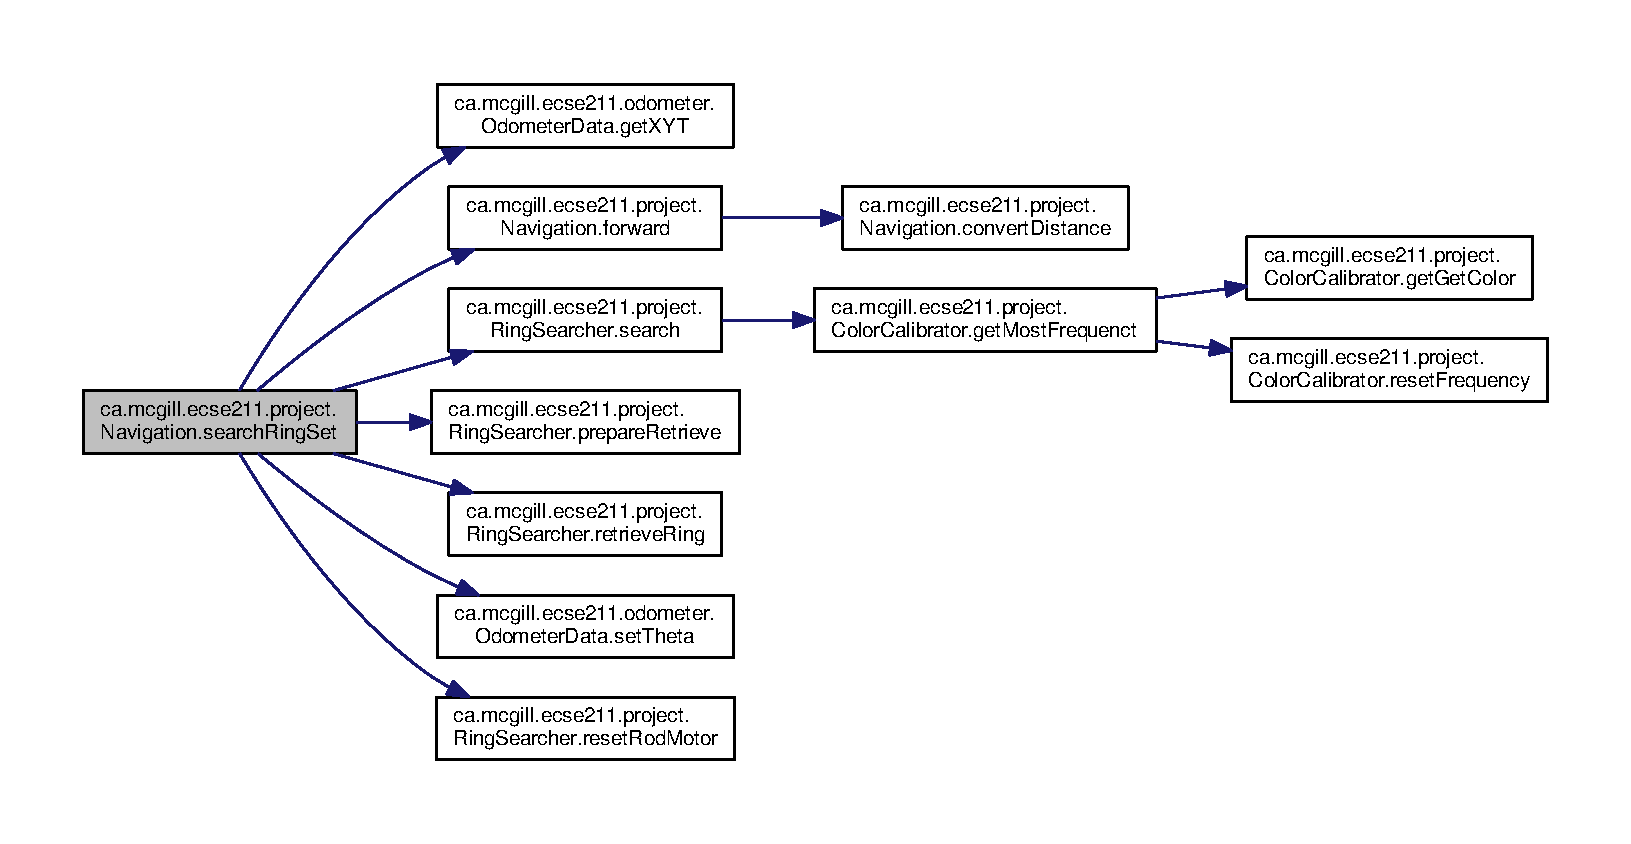
\includegraphics[width=350pt]{classca_1_1mcgill_1_1ecse211_1_1project_1_1_navigation_a1a808e665b8dd5b8e79b0580724d239c_cgraph}
\end{center}
\end{figure}
Here is the caller graph for this function\+:
\nopagebreak
\begin{figure}[H]
\begin{center}
\leavevmode
\includegraphics[width=350pt]{classca_1_1mcgill_1_1ecse211_1_1project_1_1_navigation_a1a808e665b8dd5b8e79b0580724d239c_icgraph}
\end{center}
\end{figure}
\mbox{\Hypertarget{classca_1_1mcgill_1_1ecse211_1_1project_1_1_navigation_ab01db7b8a871acd45e7dd16922abc15e}\label{classca_1_1mcgill_1_1ecse211_1_1project_1_1_navigation_ab01db7b8a871acd45e7dd16922abc15e}} 
\index{ca\+::mcgill\+::ecse211\+::project\+::\+Navigation@{ca\+::mcgill\+::ecse211\+::project\+::\+Navigation}!set\+Slow\+Acc@{set\+Slow\+Acc}}
\index{set\+Slow\+Acc@{set\+Slow\+Acc}!ca\+::mcgill\+::ecse211\+::project\+::\+Navigation@{ca\+::mcgill\+::ecse211\+::project\+::\+Navigation}}
\subsubsection{\texorpdfstring{set\+Slow\+Acc()}{setSlowAcc()}}
{\footnotesize\ttfamily void ca.\+mcgill.\+ecse211.\+project.\+Navigation.\+set\+Slow\+Acc (\begin{DoxyParamCaption}{ }\end{DoxyParamCaption})}



Definition at line 74 of file Navigation.\+java.


\begin{DoxyCode}
74                            \{
75     leftMotor.setAcceleration(N\_ACCELERATION);
76     rightMotor.setAcceleration(N\_ACCELERATION);
77   \}
\end{DoxyCode}
Here is the caller graph for this function\+:
\nopagebreak
\begin{figure}[H]
\begin{center}
\leavevmode
\includegraphics[width=350pt]{classca_1_1mcgill_1_1ecse211_1_1project_1_1_navigation_ab01db7b8a871acd45e7dd16922abc15e_icgraph}
\end{center}
\end{figure}
\mbox{\Hypertarget{classca_1_1mcgill_1_1ecse211_1_1project_1_1_navigation_ae8530d181ffd790ff9dea5eeab54b1a1}\label{classca_1_1mcgill_1_1ecse211_1_1project_1_1_navigation_ae8530d181ffd790ff9dea5eeab54b1a1}} 
\index{ca\+::mcgill\+::ecse211\+::project\+::\+Navigation@{ca\+::mcgill\+::ecse211\+::project\+::\+Navigation}!stop@{stop}}
\index{stop@{stop}!ca\+::mcgill\+::ecse211\+::project\+::\+Navigation@{ca\+::mcgill\+::ecse211\+::project\+::\+Navigation}}
\subsubsection{\texorpdfstring{stop()}{stop()}}
{\footnotesize\ttfamily void ca.\+mcgill.\+ecse211.\+project.\+Navigation.\+stop (\begin{DoxyParamCaption}{ }\end{DoxyParamCaption})}

Stop the motor 

Definition at line 645 of file Navigation.\+java.


\begin{DoxyCode}
645                      \{
646     leftMotor.stop(\textcolor{keyword}{true});
647     rightMotor.stop(\textcolor{keyword}{false});
648   \}
\end{DoxyCode}
\mbox{\Hypertarget{classca_1_1mcgill_1_1ecse211_1_1project_1_1_navigation_a3d8354490a2d8c36090d794c25d33421}\label{classca_1_1mcgill_1_1ecse211_1_1project_1_1_navigation_a3d8354490a2d8c36090d794c25d33421}} 
\index{ca\+::mcgill\+::ecse211\+::project\+::\+Navigation@{ca\+::mcgill\+::ecse211\+::project\+::\+Navigation}!travel\+To@{travel\+To}}
\index{travel\+To@{travel\+To}!ca\+::mcgill\+::ecse211\+::project\+::\+Navigation@{ca\+::mcgill\+::ecse211\+::project\+::\+Navigation}}
\subsubsection{\texorpdfstring{travel\+To()}{travelTo()}}
{\footnotesize\ttfamily void ca.\+mcgill.\+ecse211.\+project.\+Navigation.\+travel\+To (\begin{DoxyParamCaption}\item[{double}]{x,  }\item[{double}]{y,  }\item[{int}]{speed }\end{DoxyParamCaption})}

Travel to a point naively\+: by rotating the robot facing the point first and then go to the point


\begin{DoxyParams}{Parameters}
{\em x} & x coordinate of the point \\
\hline
{\em y} & y coordinate of the points \\
\hline
\end{DoxyParams}


Definition at line 101 of file Navigation.\+java.


\begin{DoxyCode}
101                                                       \{
102     \textcolor{keywordtype}{double} dX = x - odometer.\hyperlink{classca_1_1mcgill_1_1ecse211_1_1odometer_1_1_odometer_data_a8f40f0264c68f0cbed4fff1723ae7863}{getXYT}()[0];
103     \textcolor{keywordtype}{double} dY = y - odometer.\hyperlink{classca_1_1mcgill_1_1ecse211_1_1odometer_1_1_odometer_data_a8f40f0264c68f0cbed4fff1723ae7863}{getXYT}()[1];
104     \textcolor{keywordtype}{double} theta = \hyperlink{classca_1_1mcgill_1_1ecse211_1_1project_1_1_navigation_a4376e54162df8f123ca3b52e4fd2f38d}{calculateAngleTo}(x, y);
105 
106     \textcolor{comment}{// Euclidean distance calculation.}
107     \textcolor{keywordtype}{double} distance = Math.sqrt(Math.pow(dX, 2) + Math.pow(dY, 2));
108 
109     \hyperlink{classca_1_1mcgill_1_1ecse211_1_1project_1_1_navigation_a3bbe0645f2b3b3d0986b4a707fb5a00c}{turnTo}(Math.toDegrees(theta));
110     leftMotor.setSpeed(speed);
111     rightMotor.setSpeed(speed);
112     \textcolor{keywordflow}{try} \{
113       Thread.sleep(100);
114     \} \textcolor{keywordflow}{catch} (InterruptedException e) \{
115       \textcolor{comment}{// TODO Auto-generated catch block}
116       e.printStackTrace();
117     \}
118    
119 
120     leftMotor.rotate(\hyperlink{classca_1_1mcgill_1_1ecse211_1_1project_1_1_navigation_ac9e260bcd619ffa4820d7d0de7ea1c12}{convertDistance}(Game.WHEEL\_RAD, distance * Game.TILE), \textcolor{keyword}{true});
121     rightMotor.rotate(\hyperlink{classca_1_1mcgill_1_1ecse211_1_1project_1_1_navigation_ac9e260bcd619ffa4820d7d0de7ea1c12}{convertDistance}(Game.WHEEL\_RAD, distance * Game.TILE), \textcolor{keyword}{false});
122     
123   \}
\end{DoxyCode}
Here is the call graph for this function\+:
\nopagebreak
\begin{figure}[H]
\begin{center}
\leavevmode
\includegraphics[width=350pt]{classca_1_1mcgill_1_1ecse211_1_1project_1_1_navigation_a3d8354490a2d8c36090d794c25d33421_cgraph}
\end{center}
\end{figure}
Here is the caller graph for this function\+:
\nopagebreak
\begin{figure}[H]
\begin{center}
\leavevmode
\includegraphics[width=350pt]{classca_1_1mcgill_1_1ecse211_1_1project_1_1_navigation_a3d8354490a2d8c36090d794c25d33421_icgraph}
\end{center}
\end{figure}
\mbox{\Hypertarget{classca_1_1mcgill_1_1ecse211_1_1project_1_1_navigation_ae7230e905494002087416294f12cae6a}\label{classca_1_1mcgill_1_1ecse211_1_1project_1_1_navigation_ae7230e905494002087416294f12cae6a}} 
\index{ca\+::mcgill\+::ecse211\+::project\+::\+Navigation@{ca\+::mcgill\+::ecse211\+::project\+::\+Navigation}!travel\+To\+With\+Correction@{travel\+To\+With\+Correction}}
\index{travel\+To\+With\+Correction@{travel\+To\+With\+Correction}!ca\+::mcgill\+::ecse211\+::project\+::\+Navigation@{ca\+::mcgill\+::ecse211\+::project\+::\+Navigation}}
\subsubsection{\texorpdfstring{travel\+To\+With\+Correction()}{travelToWithCorrection()}}
{\footnotesize\ttfamily void ca.\+mcgill.\+ecse211.\+project.\+Navigation.\+travel\+To\+With\+Correction (\begin{DoxyParamCaption}\item[{int}]{x,  }\item[{int}]{y,  }\item[{boolean}]{avoid }\end{DoxyParamCaption})}

This method travel the robot to desired position by following the line (Always rotate 90 degree), along with a correction

When avoid=true, the nav thread will handle traveling. If you want to travel without avoidance, this is also possible. In this case, the method in the \hyperlink{classca_1_1mcgill_1_1ecse211_1_1project_1_1_navigation}{Navigation} class is used.


\begin{DoxyParams}{Parameters}
{\em x} & The x coordinate to travel to (in cm) \\
\hline
{\em y} & The y coordinate to travel to (in cm) \\
\hline
{\em avoid} & the robot will pay attention to the distance from ultrasonic sensor to avoid abstacle when navigating \\
\hline
\end{DoxyParams}


Definition at line 137 of file Navigation.\+java.


\begin{DoxyCode}
137                                                                   \{
138     \textcolor{keywordtype}{int} px = (int) Math.round(odometer.\hyperlink{classca_1_1mcgill_1_1ecse211_1_1odometer_1_1_odometer_data_a8f40f0264c68f0cbed4fff1723ae7863}{getXYT}()[0]);
139     \textcolor{keywordtype}{int} py = (int) Math.round(odometer.\hyperlink{classca_1_1mcgill_1_1ecse211_1_1odometer_1_1_odometer_data_a8f40f0264c68f0cbed4fff1723ae7863}{getXYT}()[1]);
140     \textcolor{keywordtype}{int}[] cur = \{px, py\};
141     \textcolor{keywordtype}{int}[] destination = \{x, y\};
142     ArrayList<Character> instruction = \textcolor{keyword}{new} ArrayList<Character>();
143 
144     \textcolor{comment}{// use path finder to find path based on different area the robot is at}
145     \textcolor{comment}{// OUT: instruction: contains a list of instruction for the robot to move to the destination}
146     \textcolor{keywordflow}{if} (GameParameters.getType(px, py) == GameParameters.AreaType.InStarting) \{
147       GameUtil.startingFinder.tryFindPath(cur, destination, instruction);
148     \} \textcolor{keywordflow}{else} \{
149       GameUtil.searchingFinder.tryFindPath(cur, destination, instruction);
150     \}
151 
152     \textcolor{comment}{// use the instruction modified by the pathFind to move to the destination}
153     \textcolor{keywordtype}{char} lastStep = \textcolor{charliteral}{' '};
154     \textcolor{keywordtype}{int} theta = 0;
155 
156     \textcolor{keywordflow}{while} (instruction.size() > 0) \{
157       \textcolor{keywordtype}{char} step = instruction.remove(instruction.size() - 1);
158       \textcolor{comment}{// if the step is different from the last one, rotate to corresponding rotation}
159       \textcolor{keywordflow}{if} (step != lastStep) \{
160         theta = charToRotation(step);
161         \hyperlink{classca_1_1mcgill_1_1ecse211_1_1project_1_1_navigation_a3bbe0645f2b3b3d0986b4a707fb5a00c}{turnTo}(theta);
162       \}
163 
164       \textcolor{comment}{// add a value to the robot traveled distance}
165       \textcolor{keywordflow}{if} (step == GameUtil.leftInstruction) \{
166         px--;
167       \} \textcolor{keywordflow}{else} \textcolor{keywordflow}{if} (step == GameUtil.rightInstruction) \{
168         px++;
169       \} \textcolor{keywordflow}{else} \textcolor{keywordflow}{if} (step == GameUtil.upInstruction) \{
170         py++;
171       \} \textcolor{keywordflow}{else} \{
172         py--;
173       \}
174       lastStep = step;
175 
176       \hyperlink{classca_1_1mcgill_1_1ecse211_1_1project_1_1_navigation_a48eeb9ae2da23664421e8da5642054c7}{moveWithCorrection}(1, theta);
177       \textcolor{comment}{// get the position of the robot}
178       \textcolor{keywordtype}{double}[] position = odometer.\hyperlink{classca_1_1mcgill_1_1ecse211_1_1odometer_1_1_odometer_data_a8f40f0264c68f0cbed4fff1723ae7863}{getXYT}();
179       \textcolor{keywordflow}{if} (Math.round(position[0]) == px && Math.round(position[1]) == py) \{
180         \textcolor{comment}{// this means that the robot is at the point, so set the position to the point}
181         odometer.\hyperlink{classca_1_1mcgill_1_1ecse211_1_1odometer_1_1_odometer_data_a2911d7215e47f3064defe016b46bfeef}{setX}(px);
182         odometer.\hyperlink{classca_1_1mcgill_1_1ecse211_1_1odometer_1_1_odometer_data_a82986438cd462e66520bc62bb4bd2b75}{setY}(py);
183       \} \textcolor{keywordflow}{else} \{
184         \textcolor{comment}{// otherwise some problem might happened and we are not at the desired point, push the}
185         \textcolor{comment}{// instruction back}
186         instruction.add(step);
187         \textcolor{comment}{// reset the added value to last point}
188         \textcolor{keywordflow}{if} (step == GameUtil.leftInstruction) \{
189           px++;
190         \} \textcolor{keywordflow}{else} \textcolor{keywordflow}{if} (step == GameUtil.rightInstruction) \{
191           px--;
192         \} \textcolor{keywordflow}{else} \textcolor{keywordflow}{if} (step == GameUtil.upInstruction) \{
193           py--;
194         \} \textcolor{keywordflow}{else} \{
195           py++;
196         \}
197       \}
198     \}
199   \}
\end{DoxyCode}
Here is the call graph for this function\+:
\nopagebreak
\begin{figure}[H]
\begin{center}
\leavevmode
\includegraphics[width=350pt]{classca_1_1mcgill_1_1ecse211_1_1project_1_1_navigation_ae7230e905494002087416294f12cae6a_cgraph}
\end{center}
\end{figure}
Here is the caller graph for this function\+:
\nopagebreak
\begin{figure}[H]
\begin{center}
\leavevmode
\includegraphics[width=350pt]{classca_1_1mcgill_1_1ecse211_1_1project_1_1_navigation_ae7230e905494002087416294f12cae6a_icgraph}
\end{center}
\end{figure}
\mbox{\Hypertarget{classca_1_1mcgill_1_1ecse211_1_1project_1_1_navigation_ad74286ad36d333bfaf57661837457b76}\label{classca_1_1mcgill_1_1ecse211_1_1project_1_1_navigation_ad74286ad36d333bfaf57661837457b76}} 
\index{ca\+::mcgill\+::ecse211\+::project\+::\+Navigation@{ca\+::mcgill\+::ecse211\+::project\+::\+Navigation}!turn@{turn}}
\index{turn@{turn}!ca\+::mcgill\+::ecse211\+::project\+::\+Navigation@{ca\+::mcgill\+::ecse211\+::project\+::\+Navigation}}
\subsubsection{\texorpdfstring{turn()}{turn()}}
{\footnotesize\ttfamily void ca.\+mcgill.\+ecse211.\+project.\+Navigation.\+turn (\begin{DoxyParamCaption}\item[{int}]{angle }\end{DoxyParamCaption})}

Rotate the robot by certain angle


\begin{DoxyParams}{Parameters}
{\em angle} & The angle to rotate our robot to \\
\hline
\end{DoxyParams}


Definition at line 618 of file Navigation.\+java.


\begin{DoxyCode}
618                               \{
619     leftMotor.rotate(convertAngle(Game.WHEEL\_RAD, Game.TRACK, angle), \textcolor{keyword}{true});
620     rightMotor.rotate(-convertAngle(Game.WHEEL\_RAD, Game.TRACK, angle), \textcolor{keyword}{false});
621   \}
\end{DoxyCode}
Here is the caller graph for this function\+:
\nopagebreak
\begin{figure}[H]
\begin{center}
\leavevmode
\includegraphics[width=350pt]{classca_1_1mcgill_1_1ecse211_1_1project_1_1_navigation_ad74286ad36d333bfaf57661837457b76_icgraph}
\end{center}
\end{figure}
\mbox{\Hypertarget{classca_1_1mcgill_1_1ecse211_1_1project_1_1_navigation_a3bbe0645f2b3b3d0986b4a707fb5a00c}\label{classca_1_1mcgill_1_1ecse211_1_1project_1_1_navigation_a3bbe0645f2b3b3d0986b4a707fb5a00c}} 
\index{ca\+::mcgill\+::ecse211\+::project\+::\+Navigation@{ca\+::mcgill\+::ecse211\+::project\+::\+Navigation}!turn\+To@{turn\+To}}
\index{turn\+To@{turn\+To}!ca\+::mcgill\+::ecse211\+::project\+::\+Navigation@{ca\+::mcgill\+::ecse211\+::project\+::\+Navigation}}
\subsubsection{\texorpdfstring{turn\+To()}{turnTo()}}
{\footnotesize\ttfamily synchronized void ca.\+mcgill.\+ecse211.\+project.\+Navigation.\+turn\+To (\begin{DoxyParamCaption}\item[{double}]{angle }\end{DoxyParamCaption})}

This method is where the logic for the odometer will run. Use the methods provided from the Odometer\+Data class to implement the odometer.


\begin{DoxyParams}{Parameters}
{\em angle} & The angle we want our robot to turn to (in degrees) \\
\hline
{\em async} & whether return instantaneously \\
\hline
\end{DoxyParams}


Definition at line 355 of file Navigation.\+java.


\begin{DoxyCode}
355                                                 \{
356     \textcolor{keywordtype}{double} dTheta;
357 
358     dTheta = angle - odometer.\hyperlink{classca_1_1mcgill_1_1ecse211_1_1odometer_1_1_odometer_data_a8f40f0264c68f0cbed4fff1723ae7863}{getXYT}()[2];
359     \textcolor{keywordflow}{if} (dTheta < 0)
360       dTheta += 360;
361 
362     \textcolor{comment}{// TURN RIGHT}
363     \textcolor{keywordflow}{if} (dTheta > 180) \{
364       leftMotor.setSpeed(ROTATE\_SPEED);
365       rightMotor.setSpeed(ROTATE\_SPEED);
366       \textcolor{keywordflow}{try} \{
367         Thread.sleep(100);
368       \} \textcolor{keywordflow}{catch} (InterruptedException e) \{
369         \textcolor{comment}{// TODO Auto-generated catch block}
370         e.printStackTrace();
371       \}
372       leftMotor.rotate(-convertAngle(Game.WHEEL\_RAD, Game.TRACK, 360 - dTheta), \textcolor{keyword}{true});
373       rightMotor.rotate(convertAngle(Game.WHEEL\_RAD, Game.TRACK, 360 - dTheta), \textcolor{keyword}{false});
374     \}
375     \textcolor{comment}{// TURN LEFT}
376     \textcolor{keywordflow}{else} \{
377       leftMotor.setSpeed(ROTATE\_SPEED);
378       rightMotor.setSpeed(ROTATE\_SPEED);
379       \textcolor{keywordflow}{try} \{
380         Thread.sleep(100);
381       \} \textcolor{keywordflow}{catch} (InterruptedException e) \{
382         \textcolor{comment}{// TODO Auto-generated catch block}
383         e.printStackTrace();
384       \}
385       leftMotor.rotate(convertAngle(Game.WHEEL\_RAD, Game.TRACK, dTheta), \textcolor{keyword}{true});
386       rightMotor.rotate(-convertAngle(Game.WHEEL\_RAD, Game.TRACK, dTheta), \textcolor{keyword}{false});
387     \}
388   \}
\end{DoxyCode}
Here is the call graph for this function\+:
\nopagebreak
\begin{figure}[H]
\begin{center}
\leavevmode
\includegraphics[width=350pt]{classca_1_1mcgill_1_1ecse211_1_1project_1_1_navigation_a3bbe0645f2b3b3d0986b4a707fb5a00c_cgraph}
\end{center}
\end{figure}
Here is the caller graph for this function\+:
\nopagebreak
\begin{figure}[H]
\begin{center}
\leavevmode
\includegraphics[width=350pt]{classca_1_1mcgill_1_1ecse211_1_1project_1_1_navigation_a3bbe0645f2b3b3d0986b4a707fb5a00c_icgraph}
\end{center}
\end{figure}


The documentation for this class was generated from the following file\+:\begin{DoxyCompactItemize}
\item 
/home/ccc/\+Final\+Project/src/ca/mcgill/ecse211/project/\hyperlink{_navigation_8java}{Navigation.\+java}\end{DoxyCompactItemize}

\hypertarget{classca_1_1mcgill_1_1ecse211_1_1odometer_1_1_odometer}{}\section{ca.\+mcgill.\+ecse211.\+odometer.\+Odometer Class Reference}
\label{classca_1_1mcgill_1_1ecse211_1_1odometer_1_1_odometer}\index{ca.\+mcgill.\+ecse211.\+odometer.\+Odometer@{ca.\+mcgill.\+ecse211.\+odometer.\+Odometer}}


Inheritance diagram for ca.\+mcgill.\+ecse211.\+odometer.\+Odometer\+:
\nopagebreak
\begin{figure}[H]
\begin{center}
\leavevmode
\includegraphics[width=298pt]{classca_1_1mcgill_1_1ecse211_1_1odometer_1_1_odometer__inherit__graph}
\end{center}
\end{figure}


Collaboration diagram for ca.\+mcgill.\+ecse211.\+odometer.\+Odometer\+:
\nopagebreak
\begin{figure}[H]
\begin{center}
\leavevmode
\includegraphics[width=298pt]{classca_1_1mcgill_1_1ecse211_1_1odometer_1_1_odometer__coll__graph}
\end{center}
\end{figure}
\subsection*{Public Member Functions}
\begin{DoxyCompactItemize}
\item 
void \hyperlink{classca_1_1mcgill_1_1ecse211_1_1odometer_1_1_odometer_af0ff4c5121973a8310cf986e25fa0d87}{run} ()
\end{DoxyCompactItemize}
\subsection*{Static Public Member Functions}
\begin{DoxyCompactItemize}
\item 
static synchronized \hyperlink{classca_1_1mcgill_1_1ecse211_1_1odometer_1_1_odometer}{Odometer} \hyperlink{classca_1_1mcgill_1_1ecse211_1_1odometer_1_1_odometer_a99171f11e34dea918fa9dd069d721439}{get\+Odometer} (E\+V3\+Large\+Regulated\+Motor left\+Motor, E\+V3\+Large\+Regulated\+Motor right\+Motor, final double T\+R\+A\+CK, final double W\+H\+E\+E\+L\+\_\+\+R\+AD)  throws Odometer\+Exceptions 
\item 
static synchronized \hyperlink{classca_1_1mcgill_1_1ecse211_1_1odometer_1_1_odometer}{Odometer} \hyperlink{classca_1_1mcgill_1_1ecse211_1_1odometer_1_1_odometer_a4e069b5a96cd43b29af0785244a99b51}{get\+Odometer} ()  throws Odometer\+Exceptions 
\end{DoxyCompactItemize}
\subsection*{Additional Inherited Members}


\subsection{Detailed Description}
This class implements odometry on our robot.

\begin{DoxyAuthor}{Author}
Caspar Cedro 

Percy Chen 

Patrick Erath 

Anssam Ghezala 

Susan Matuszewski 

Kamy Moussavi Kafi 
\end{DoxyAuthor}


Definition at line 26 of file Odometer.\+java.



\subsection{Member Function Documentation}
\mbox{\Hypertarget{classca_1_1mcgill_1_1ecse211_1_1odometer_1_1_odometer_a99171f11e34dea918fa9dd069d721439}\label{classca_1_1mcgill_1_1ecse211_1_1odometer_1_1_odometer_a99171f11e34dea918fa9dd069d721439}} 
\index{ca\+::mcgill\+::ecse211\+::odometer\+::\+Odometer@{ca\+::mcgill\+::ecse211\+::odometer\+::\+Odometer}!get\+Odometer@{get\+Odometer}}
\index{get\+Odometer@{get\+Odometer}!ca\+::mcgill\+::ecse211\+::odometer\+::\+Odometer@{ca\+::mcgill\+::ecse211\+::odometer\+::\+Odometer}}
\subsubsection{\texorpdfstring{get\+Odometer()}{getOdometer()}\hspace{0.1cm}{\footnotesize\ttfamily [1/2]}}
{\footnotesize\ttfamily static synchronized \hyperlink{classca_1_1mcgill_1_1ecse211_1_1odometer_1_1_odometer}{Odometer} ca.\+mcgill.\+ecse211.\+odometer.\+Odometer.\+get\+Odometer (\begin{DoxyParamCaption}\item[{E\+V3\+Large\+Regulated\+Motor}]{left\+Motor,  }\item[{E\+V3\+Large\+Regulated\+Motor}]{right\+Motor,  }\item[{final double}]{T\+R\+A\+CK,  }\item[{final double}]{W\+H\+E\+E\+L\+\_\+\+R\+AD }\end{DoxyParamCaption}) throws \hyperlink{classca_1_1mcgill_1_1ecse211_1_1odometer_1_1_odometer_exceptions}{Odometer\+Exceptions}\hspace{0.3cm}{\ttfamily [static]}}

This method is meant to ensure only one instance of the odometer is used throughout the code.


\begin{DoxyParams}{Parameters}
{\em left\+Motor} & The E\+V3\+Large\+Regulated\+Motor instance for our left motor \\
\hline
{\em right\+Motor} & The E\+V3\+Large\+Regulated\+Motor instance for our right motor \\
\hline
\end{DoxyParams}
\begin{DoxyReturn}{Returns}
new or existing \hyperlink{classca_1_1mcgill_1_1ecse211_1_1odometer_1_1_odometer}{Odometer} Object 
\end{DoxyReturn}

\begin{DoxyExceptions}{Exceptions}
{\em \hyperlink{classca_1_1mcgill_1_1ecse211_1_1odometer_1_1_odometer_exceptions}{Odometer\+Exceptions}} & \\
\hline
\end{DoxyExceptions}


Definition at line 79 of file Odometer.\+java.

Here is the caller graph for this function\+:
\nopagebreak
\begin{figure}[H]
\begin{center}
\leavevmode
\includegraphics[width=350pt]{classca_1_1mcgill_1_1ecse211_1_1odometer_1_1_odometer_a99171f11e34dea918fa9dd069d721439_icgraph}
\end{center}
\end{figure}
\mbox{\Hypertarget{classca_1_1mcgill_1_1ecse211_1_1odometer_1_1_odometer_a4e069b5a96cd43b29af0785244a99b51}\label{classca_1_1mcgill_1_1ecse211_1_1odometer_1_1_odometer_a4e069b5a96cd43b29af0785244a99b51}} 
\index{ca\+::mcgill\+::ecse211\+::odometer\+::\+Odometer@{ca\+::mcgill\+::ecse211\+::odometer\+::\+Odometer}!get\+Odometer@{get\+Odometer}}
\index{get\+Odometer@{get\+Odometer}!ca\+::mcgill\+::ecse211\+::odometer\+::\+Odometer@{ca\+::mcgill\+::ecse211\+::odometer\+::\+Odometer}}
\subsubsection{\texorpdfstring{get\+Odometer()}{getOdometer()}\hspace{0.1cm}{\footnotesize\ttfamily [2/2]}}
{\footnotesize\ttfamily static synchronized \hyperlink{classca_1_1mcgill_1_1ecse211_1_1odometer_1_1_odometer}{Odometer} ca.\+mcgill.\+ecse211.\+odometer.\+Odometer.\+get\+Odometer (\begin{DoxyParamCaption}{ }\end{DoxyParamCaption}) throws \hyperlink{classca_1_1mcgill_1_1ecse211_1_1odometer_1_1_odometer_exceptions}{Odometer\+Exceptions}\hspace{0.3cm}{\ttfamily [static]}}

This class is meant to return the existing \hyperlink{classca_1_1mcgill_1_1ecse211_1_1odometer_1_1_odometer}{Odometer} Object. It is meant to be used only if an odometer object has been created

\begin{DoxyReturn}{Returns}
error if no previous odometer exists 
\end{DoxyReturn}


Definition at line 96 of file Odometer.\+java.

\mbox{\Hypertarget{classca_1_1mcgill_1_1ecse211_1_1odometer_1_1_odometer_af0ff4c5121973a8310cf986e25fa0d87}\label{classca_1_1mcgill_1_1ecse211_1_1odometer_1_1_odometer_af0ff4c5121973a8310cf986e25fa0d87}} 
\index{ca\+::mcgill\+::ecse211\+::odometer\+::\+Odometer@{ca\+::mcgill\+::ecse211\+::odometer\+::\+Odometer}!run@{run}}
\index{run@{run}!ca\+::mcgill\+::ecse211\+::odometer\+::\+Odometer@{ca\+::mcgill\+::ecse211\+::odometer\+::\+Odometer}}
\subsubsection{\texorpdfstring{run()}{run()}}
{\footnotesize\ttfamily void ca.\+mcgill.\+ecse211.\+odometer.\+Odometer.\+run (\begin{DoxyParamCaption}{ }\end{DoxyParamCaption})}

This method is called when our \hyperlink{classca_1_1mcgill_1_1ecse211_1_1odometer_1_1_odometer}{Odometer} object is started as a thread and begins to keep track of motor rotations 

Definition at line 109 of file Odometer.\+java.

Here is the call graph for this function\+:
\nopagebreak
\begin{figure}[H]
\begin{center}
\leavevmode
\includegraphics[width=350pt]{classca_1_1mcgill_1_1ecse211_1_1odometer_1_1_odometer_af0ff4c5121973a8310cf986e25fa0d87_cgraph}
\end{center}
\end{figure}


The documentation for this class was generated from the following file\+:\begin{DoxyCompactItemize}
\item 
/home/ccc/\+Final\+Project/src/ca/mcgill/ecse211/odometer/Odometer.\+java\end{DoxyCompactItemize}

\hypertarget{classca_1_1mcgill_1_1ecse211_1_1odometer_1_1_odometer_data}{}\section{ca.\+mcgill.\+ecse211.\+odometer.\+Odometer\+Data Class Reference}
\label{classca_1_1mcgill_1_1ecse211_1_1odometer_1_1_odometer_data}\index{ca.\+mcgill.\+ecse211.\+odometer.\+Odometer\+Data@{ca.\+mcgill.\+ecse211.\+odometer.\+Odometer\+Data}}


Inheritance diagram for ca.\+mcgill.\+ecse211.\+odometer.\+Odometer\+Data\+:\nopagebreak
\begin{figure}[H]
\begin{center}
\leavevmode
\includegraphics[width=222pt]{classca_1_1mcgill_1_1ecse211_1_1odometer_1_1_odometer_data__inherit__graph}
\end{center}
\end{figure}
\subsection*{Public Member Functions}
\begin{DoxyCompactItemize}
\item 
double \mbox{[}$\,$\mbox{]} \hyperlink{classca_1_1mcgill_1_1ecse211_1_1odometer_1_1_odometer_data_a8f40f0264c68f0cbed4fff1723ae7863}{get\+X\+YT} ()
\item 
void \hyperlink{classca_1_1mcgill_1_1ecse211_1_1odometer_1_1_odometer_data_aaa06f190d634299fcb1b97a1891dad85}{update} (double dx, double dy, double dtheta)
\item 
void \hyperlink{classca_1_1mcgill_1_1ecse211_1_1odometer_1_1_odometer_data_a2ebc18a13aea6276122d9ef4ee100bb9}{set\+X\+YT} (double x, double y, double theta)
\item 
void \hyperlink{classca_1_1mcgill_1_1ecse211_1_1odometer_1_1_odometer_data_a2911d7215e47f3064defe016b46bfeef}{setX} (double x)
\item 
void \hyperlink{classca_1_1mcgill_1_1ecse211_1_1odometer_1_1_odometer_data_a82986438cd462e66520bc62bb4bd2b75}{setY} (double y)
\item 
void \hyperlink{classca_1_1mcgill_1_1ecse211_1_1odometer_1_1_odometer_data_a419b8f07c2c5374411c8e62298e9a402}{set\+Theta} (double theta)
\end{DoxyCompactItemize}
\subsection*{Static Public Member Functions}
\begin{DoxyCompactItemize}
\item 
static synchronized \hyperlink{classca_1_1mcgill_1_1ecse211_1_1odometer_1_1_odometer_data}{Odometer\+Data} \hyperlink{classca_1_1mcgill_1_1ecse211_1_1odometer_1_1_odometer_data_afff2d760dd1f861b580f3eacef37f1cc}{get\+Odometer\+Data} ()  throws Odometer\+Exceptions 
\end{DoxyCompactItemize}
\subsection*{Protected Member Functions}
\begin{DoxyCompactItemize}
\item 
\hyperlink{classca_1_1mcgill_1_1ecse211_1_1odometer_1_1_odometer_data_a91412854b75c41bf3af7c8892ec0fe87}{Odometer\+Data} ()
\end{DoxyCompactItemize}


\subsection{Detailed Description}
This class stores and provides thread safe access to data required used by the \hyperlink{classca_1_1mcgill_1_1ecse211_1_1odometer_1_1_odometer}{Odometer} classes.

\begin{DoxyAuthor}{Author}
Caspar Cedro 

Percy Chen 

Patrick Erath 

Anssam Ghezala 

Susan Matuszewski 

Kamy Moussavi Kafi 
\end{DoxyAuthor}


Definition at line 17 of file Odometer\+Data.\+java.



\subsection{Constructor \& Destructor Documentation}
\mbox{\Hypertarget{classca_1_1mcgill_1_1ecse211_1_1odometer_1_1_odometer_data_a91412854b75c41bf3af7c8892ec0fe87}\label{classca_1_1mcgill_1_1ecse211_1_1odometer_1_1_odometer_data_a91412854b75c41bf3af7c8892ec0fe87}} 
\index{ca\+::mcgill\+::ecse211\+::odometer\+::\+Odometer\+Data@{ca\+::mcgill\+::ecse211\+::odometer\+::\+Odometer\+Data}!Odometer\+Data@{Odometer\+Data}}
\index{Odometer\+Data@{Odometer\+Data}!ca\+::mcgill\+::ecse211\+::odometer\+::\+Odometer\+Data@{ca\+::mcgill\+::ecse211\+::odometer\+::\+Odometer\+Data}}
\subsubsection{\texorpdfstring{Odometer\+Data()}{OdometerData()}}
{\footnotesize\ttfamily ca.\+mcgill.\+ecse211.\+odometer.\+Odometer\+Data.\+Odometer\+Data (\begin{DoxyParamCaption}{ }\end{DoxyParamCaption})\hspace{0.3cm}{\ttfamily [protected]}}

This is the class constructor for the \hyperlink{classca_1_1mcgill_1_1ecse211_1_1odometer_1_1_odometer_data}{Odometer\+Data} class. It cannot be instantiated externally. A factory is used instead such that only one instance of this class is ever created. 

Definition at line 47 of file Odometer\+Data.\+java.


\begin{DoxyCode}
47                            \{
48     this.x = 0;
49     this.y = 0;
50     this.theta = 0;
51   \}
\end{DoxyCode}
Here is the caller graph for this function\+:\nopagebreak
\begin{figure}[H]
\begin{center}
\leavevmode
\includegraphics[width=350pt]{classca_1_1mcgill_1_1ecse211_1_1odometer_1_1_odometer_data_a91412854b75c41bf3af7c8892ec0fe87_icgraph}
\end{center}
\end{figure}


\subsection{Member Function Documentation}
\mbox{\Hypertarget{classca_1_1mcgill_1_1ecse211_1_1odometer_1_1_odometer_data_afff2d760dd1f861b580f3eacef37f1cc}\label{classca_1_1mcgill_1_1ecse211_1_1odometer_1_1_odometer_data_afff2d760dd1f861b580f3eacef37f1cc}} 
\index{ca\+::mcgill\+::ecse211\+::odometer\+::\+Odometer\+Data@{ca\+::mcgill\+::ecse211\+::odometer\+::\+Odometer\+Data}!get\+Odometer\+Data@{get\+Odometer\+Data}}
\index{get\+Odometer\+Data@{get\+Odometer\+Data}!ca\+::mcgill\+::ecse211\+::odometer\+::\+Odometer\+Data@{ca\+::mcgill\+::ecse211\+::odometer\+::\+Odometer\+Data}}
\subsubsection{\texorpdfstring{get\+Odometer\+Data()}{getOdometerData()}}
{\footnotesize\ttfamily static synchronized \hyperlink{classca_1_1mcgill_1_1ecse211_1_1odometer_1_1_odometer_data}{Odometer\+Data} ca.\+mcgill.\+ecse211.\+odometer.\+Odometer\+Data.\+get\+Odometer\+Data (\begin{DoxyParamCaption}{ }\end{DoxyParamCaption}) throws \hyperlink{classca_1_1mcgill_1_1ecse211_1_1odometer_1_1_odometer_exceptions}{Odometer\+Exceptions}\hspace{0.3cm}{\ttfamily [static]}}

This method returns an \hyperlink{classca_1_1mcgill_1_1ecse211_1_1odometer_1_1_odometer_data}{Odometer\+Data} instance and makes sure that only one instance is ever created.

\begin{DoxyReturn}{Returns}
An \hyperlink{classca_1_1mcgill_1_1ecse211_1_1odometer_1_1_odometer_data}{Odometer\+Data} object 
\end{DoxyReturn}

\begin{DoxyExceptions}{Exceptions}
{\em \hyperlink{classca_1_1mcgill_1_1ecse211_1_1odometer_1_1_odometer_exceptions}{Odometer\+Exceptions}} & \\
\hline
\end{DoxyExceptions}


Definition at line 60 of file Odometer\+Data.\+java.


\begin{DoxyCode}
60                                                                                       \{
61     \textcolor{keywordflow}{if} (odoData != null) \{ \textcolor{comment}{// Return existing object}
62       \textcolor{keywordflow}{return} odoData;
63     \} \textcolor{keywordflow}{else} \textcolor{keywordflow}{if} (numberOfIntances < MAX\_INSTANCES) \{
64       \textcolor{comment}{// create object and return it}
65       odoData = \textcolor{keyword}{new} \hyperlink{classca_1_1mcgill_1_1ecse211_1_1odometer_1_1_odometer_data_a91412854b75c41bf3af7c8892ec0fe87}{OdometerData}();
66       numberOfIntances += 1;
67       \textcolor{keywordflow}{return} odoData;
68     \} \textcolor{keywordflow}{else} \{
69       \textcolor{keywordflow}{throw} \textcolor{keyword}{new} OdometerExceptions(\textcolor{stringliteral}{"Only one intance of the Odometer can be created."});
70     \}
71   \}
\end{DoxyCode}
Here is the call graph for this function\+:\nopagebreak
\begin{figure}[H]
\begin{center}
\leavevmode
\includegraphics[width=350pt]{classca_1_1mcgill_1_1ecse211_1_1odometer_1_1_odometer_data_afff2d760dd1f861b580f3eacef37f1cc_cgraph}
\end{center}
\end{figure}
\mbox{\Hypertarget{classca_1_1mcgill_1_1ecse211_1_1odometer_1_1_odometer_data_a8f40f0264c68f0cbed4fff1723ae7863}\label{classca_1_1mcgill_1_1ecse211_1_1odometer_1_1_odometer_data_a8f40f0264c68f0cbed4fff1723ae7863}} 
\index{ca\+::mcgill\+::ecse211\+::odometer\+::\+Odometer\+Data@{ca\+::mcgill\+::ecse211\+::odometer\+::\+Odometer\+Data}!get\+X\+YT@{get\+X\+YT}}
\index{get\+X\+YT@{get\+X\+YT}!ca\+::mcgill\+::ecse211\+::odometer\+::\+Odometer\+Data@{ca\+::mcgill\+::ecse211\+::odometer\+::\+Odometer\+Data}}
\subsubsection{\texorpdfstring{get\+X\+Y\+T()}{getXYT()}}
{\footnotesize\ttfamily double \mbox{[}$\,$\mbox{]} ca.\+mcgill.\+ecse211.\+odometer.\+Odometer\+Data.\+get\+X\+YT (\begin{DoxyParamCaption}{ }\end{DoxyParamCaption})}

This method returns the \hyperlink{classca_1_1mcgill_1_1ecse211_1_1odometer_1_1_odometer}{Odometer} data. Writes the current position and orientation of the robot onto the odo\+Data array. odo\+Data\mbox{[}0\mbox{]} = x, odo\+Data\mbox{[}1\mbox{]} = y; odo\+Data\mbox{[}2\mbox{]} = theta;


\begin{DoxyParams}{Parameters}
{\em position} & the array to store the odometer data \\
\hline
\end{DoxyParams}
\begin{DoxyReturn}{Returns}
the odometer data. 
\end{DoxyReturn}


Definition at line 81 of file Odometer\+Data.\+java.


\begin{DoxyCode}
81                            \{
82     \textcolor{keywordtype}{double}[] position = \textcolor{keyword}{new} \textcolor{keywordtype}{double}[4];
83     lock.lock();
84     \textcolor{keywordflow}{try} \{
85       \textcolor{keywordflow}{while} (isReseting) \{ \textcolor{comment}{// If a reset operation is being executed, wait}
86         \textcolor{comment}{// until it is over.}
87         doneReseting.await(); \textcolor{comment}{// Using await() is lighter on the CPU}
88         \textcolor{comment}{// than simple busy wait.}
89       \}
90 
91       position[0] = x;
92       position[1] = y;
93       position[2] = theta;
94 
95     \} \textcolor{keywordflow}{catch} (InterruptedException e) \{
96       \textcolor{comment}{// Print exception to screen}
97       e.printStackTrace();
98     \} \textcolor{keywordflow}{finally} \{
99       lock.unlock();
100     \}
101 
102     \textcolor{keywordflow}{return} position;
103   \}
\end{DoxyCode}
Here is the caller graph for this function\+:\nopagebreak
\begin{figure}[H]
\begin{center}
\leavevmode
\includegraphics[width=350pt]{classca_1_1mcgill_1_1ecse211_1_1odometer_1_1_odometer_data_a8f40f0264c68f0cbed4fff1723ae7863_icgraph}
\end{center}
\end{figure}
\mbox{\Hypertarget{classca_1_1mcgill_1_1ecse211_1_1odometer_1_1_odometer_data_a419b8f07c2c5374411c8e62298e9a402}\label{classca_1_1mcgill_1_1ecse211_1_1odometer_1_1_odometer_data_a419b8f07c2c5374411c8e62298e9a402}} 
\index{ca\+::mcgill\+::ecse211\+::odometer\+::\+Odometer\+Data@{ca\+::mcgill\+::ecse211\+::odometer\+::\+Odometer\+Data}!set\+Theta@{set\+Theta}}
\index{set\+Theta@{set\+Theta}!ca\+::mcgill\+::ecse211\+::odometer\+::\+Odometer\+Data@{ca\+::mcgill\+::ecse211\+::odometer\+::\+Odometer\+Data}}
\subsubsection{\texorpdfstring{set\+Theta()}{setTheta()}}
{\footnotesize\ttfamily void ca.\+mcgill.\+ecse211.\+odometer.\+Odometer\+Data.\+set\+Theta (\begin{DoxyParamCaption}\item[{double}]{theta }\end{DoxyParamCaption})}

Overrides theta. Use for odometry correction.


\begin{DoxyParams}{Parameters}
{\em theta} & the value of theta \\
\hline
\end{DoxyParams}


Definition at line 194 of file Odometer\+Data.\+java.


\begin{DoxyCode}
194                                      \{
195     lock.lock();
196     isReseting = \textcolor{keyword}{true};
197     \textcolor{keywordflow}{try} \{
198       this.theta = theta;
199       isReseting = \textcolor{keyword}{false}; \textcolor{comment}{// Done reseting}
200       doneReseting.signalAll(); \textcolor{comment}{// Let the other threads know that you are}
201                                 \textcolor{comment}{// done reseting}
202     \} \textcolor{keywordflow}{finally} \{
203       lock.unlock();
204     \}
205   \}
\end{DoxyCode}
Here is the caller graph for this function\+:\nopagebreak
\begin{figure}[H]
\begin{center}
\leavevmode
\includegraphics[width=350pt]{classca_1_1mcgill_1_1ecse211_1_1odometer_1_1_odometer_data_a419b8f07c2c5374411c8e62298e9a402_icgraph}
\end{center}
\end{figure}
\mbox{\Hypertarget{classca_1_1mcgill_1_1ecse211_1_1odometer_1_1_odometer_data_a2911d7215e47f3064defe016b46bfeef}\label{classca_1_1mcgill_1_1ecse211_1_1odometer_1_1_odometer_data_a2911d7215e47f3064defe016b46bfeef}} 
\index{ca\+::mcgill\+::ecse211\+::odometer\+::\+Odometer\+Data@{ca\+::mcgill\+::ecse211\+::odometer\+::\+Odometer\+Data}!setX@{setX}}
\index{setX@{setX}!ca\+::mcgill\+::ecse211\+::odometer\+::\+Odometer\+Data@{ca\+::mcgill\+::ecse211\+::odometer\+::\+Odometer\+Data}}
\subsubsection{\texorpdfstring{set\+X()}{setX()}}
{\footnotesize\ttfamily void ca.\+mcgill.\+ecse211.\+odometer.\+Odometer\+Data.\+setX (\begin{DoxyParamCaption}\item[{double}]{x }\end{DoxyParamCaption})}

Overrides x. Use for odometry correction.


\begin{DoxyParams}{Parameters}
{\em x} & the value of x \\
\hline
\end{DoxyParams}


Definition at line 158 of file Odometer\+Data.\+java.


\begin{DoxyCode}
158                              \{
159     lock.lock();
160     isReseting = \textcolor{keyword}{true};
161     \textcolor{keywordflow}{try} \{
162       this.x = x;
163       isReseting = \textcolor{keyword}{false}; \textcolor{comment}{// Done reseting}
164       doneReseting.signalAll(); \textcolor{comment}{// Let the other threads know that you are}
165                                 \textcolor{comment}{// done reseting}
166     \} \textcolor{keywordflow}{finally} \{
167       lock.unlock();
168     \}
169   \}
\end{DoxyCode}
Here is the caller graph for this function\+:\nopagebreak
\begin{figure}[H]
\begin{center}
\leavevmode
\includegraphics[width=350pt]{classca_1_1mcgill_1_1ecse211_1_1odometer_1_1_odometer_data_a2911d7215e47f3064defe016b46bfeef_icgraph}
\end{center}
\end{figure}
\mbox{\Hypertarget{classca_1_1mcgill_1_1ecse211_1_1odometer_1_1_odometer_data_a2ebc18a13aea6276122d9ef4ee100bb9}\label{classca_1_1mcgill_1_1ecse211_1_1odometer_1_1_odometer_data_a2ebc18a13aea6276122d9ef4ee100bb9}} 
\index{ca\+::mcgill\+::ecse211\+::odometer\+::\+Odometer\+Data@{ca\+::mcgill\+::ecse211\+::odometer\+::\+Odometer\+Data}!set\+X\+YT@{set\+X\+YT}}
\index{set\+X\+YT@{set\+X\+YT}!ca\+::mcgill\+::ecse211\+::odometer\+::\+Odometer\+Data@{ca\+::mcgill\+::ecse211\+::odometer\+::\+Odometer\+Data}}
\subsubsection{\texorpdfstring{set\+X\+Y\+T()}{setXYT()}}
{\footnotesize\ttfamily void ca.\+mcgill.\+ecse211.\+odometer.\+Odometer\+Data.\+set\+X\+YT (\begin{DoxyParamCaption}\item[{double}]{x,  }\item[{double}]{y,  }\item[{double}]{theta }\end{DoxyParamCaption})}

Overrides the values of x, y and theta. Use for odometry correction.


\begin{DoxyParams}{Parameters}
{\em x} & the value of x \\
\hline
{\em y} & the value of y \\
\hline
{\em theta} & the value of theta \\
\hline
\end{DoxyParams}


Definition at line 138 of file Odometer\+Data.\+java.


\begin{DoxyCode}
138                                                        \{
139     lock.lock();
140     isReseting = \textcolor{keyword}{true};
141     \textcolor{keywordflow}{try} \{
142       this.x = x;
143       this.y = y;
144       this.theta = theta;
145       isReseting = \textcolor{keyword}{false}; \textcolor{comment}{// Done reseting}
146       doneReseting.signalAll(); \textcolor{comment}{// Let the other threads know that you are}
147                                 \textcolor{comment}{// done reseting}
148     \} \textcolor{keywordflow}{finally} \{
149       lock.unlock();
150     \}
151   \}
\end{DoxyCode}
Here is the caller graph for this function\+:\nopagebreak
\begin{figure}[H]
\begin{center}
\leavevmode
\includegraphics[width=350pt]{classca_1_1mcgill_1_1ecse211_1_1odometer_1_1_odometer_data_a2ebc18a13aea6276122d9ef4ee100bb9_icgraph}
\end{center}
\end{figure}
\mbox{\Hypertarget{classca_1_1mcgill_1_1ecse211_1_1odometer_1_1_odometer_data_a82986438cd462e66520bc62bb4bd2b75}\label{classca_1_1mcgill_1_1ecse211_1_1odometer_1_1_odometer_data_a82986438cd462e66520bc62bb4bd2b75}} 
\index{ca\+::mcgill\+::ecse211\+::odometer\+::\+Odometer\+Data@{ca\+::mcgill\+::ecse211\+::odometer\+::\+Odometer\+Data}!setY@{setY}}
\index{setY@{setY}!ca\+::mcgill\+::ecse211\+::odometer\+::\+Odometer\+Data@{ca\+::mcgill\+::ecse211\+::odometer\+::\+Odometer\+Data}}
\subsubsection{\texorpdfstring{set\+Y()}{setY()}}
{\footnotesize\ttfamily void ca.\+mcgill.\+ecse211.\+odometer.\+Odometer\+Data.\+setY (\begin{DoxyParamCaption}\item[{double}]{y }\end{DoxyParamCaption})}

Overrides y. Use for odometry correction.


\begin{DoxyParams}{Parameters}
{\em y} & the value of y \\
\hline
\end{DoxyParams}


Definition at line 176 of file Odometer\+Data.\+java.


\begin{DoxyCode}
176                              \{
177     lock.lock();
178     isReseting = \textcolor{keyword}{true};
179     \textcolor{keywordflow}{try} \{
180       this.y = y;
181       isReseting = \textcolor{keyword}{false}; \textcolor{comment}{// Done reseting}
182       doneReseting.signalAll(); \textcolor{comment}{// Let the other threads know that you are}
183                                 \textcolor{comment}{// done reseting}
184     \} \textcolor{keywordflow}{finally} \{
185       lock.unlock();
186     \}
187   \}
\end{DoxyCode}
Here is the caller graph for this function\+:\nopagebreak
\begin{figure}[H]
\begin{center}
\leavevmode
\includegraphics[width=350pt]{classca_1_1mcgill_1_1ecse211_1_1odometer_1_1_odometer_data_a82986438cd462e66520bc62bb4bd2b75_icgraph}
\end{center}
\end{figure}
\mbox{\Hypertarget{classca_1_1mcgill_1_1ecse211_1_1odometer_1_1_odometer_data_aaa06f190d634299fcb1b97a1891dad85}\label{classca_1_1mcgill_1_1ecse211_1_1odometer_1_1_odometer_data_aaa06f190d634299fcb1b97a1891dad85}} 
\index{ca\+::mcgill\+::ecse211\+::odometer\+::\+Odometer\+Data@{ca\+::mcgill\+::ecse211\+::odometer\+::\+Odometer\+Data}!update@{update}}
\index{update@{update}!ca\+::mcgill\+::ecse211\+::odometer\+::\+Odometer\+Data@{ca\+::mcgill\+::ecse211\+::odometer\+::\+Odometer\+Data}}
\subsubsection{\texorpdfstring{update()}{update()}}
{\footnotesize\ttfamily void ca.\+mcgill.\+ecse211.\+odometer.\+Odometer\+Data.\+update (\begin{DoxyParamCaption}\item[{double}]{dx,  }\item[{double}]{dy,  }\item[{double}]{dtheta }\end{DoxyParamCaption})}

Adds dx, dy and dtheta to the current values of x, y and theta, respectively. Useful for odometry.


\begin{DoxyParams}{Parameters}
{\em dx} & \\
\hline
{\em dy} & \\
\hline
{\em dtheta} & \\
\hline
\end{DoxyParams}


Definition at line 113 of file Odometer\+Data.\+java.


\begin{DoxyCode}
113                                                           \{
114     lock.lock();
115     isReseting = \textcolor{keyword}{true};
116     \textcolor{keywordflow}{try} \{
117       x += dx;
118       y += dy;
119       theta = (theta + (360 + dtheta) % 360) % 360; \textcolor{comment}{// keeps the updates}
120                                                     \textcolor{comment}{// within 360}
121                                                     \textcolor{comment}{// degrees}
122       isReseting = \textcolor{keyword}{false}; \textcolor{comment}{// Done reseting}
123       doneReseting.signalAll(); \textcolor{comment}{// Let the other threads know that you are}
124                                 \textcolor{comment}{// done reseting}
125     \} \textcolor{keywordflow}{finally} \{
126       lock.unlock();
127     \}
128 
129   \}
\end{DoxyCode}
Here is the caller graph for this function\+:\nopagebreak
\begin{figure}[H]
\begin{center}
\leavevmode
\includegraphics[width=350pt]{classca_1_1mcgill_1_1ecse211_1_1odometer_1_1_odometer_data_aaa06f190d634299fcb1b97a1891dad85_icgraph}
\end{center}
\end{figure}


The documentation for this class was generated from the following file\+:\begin{DoxyCompactItemize}
\item 
/home/ccc/\+Final\+Project/src/ca/mcgill/ecse211/odometer/\hyperlink{_odometer_data_8java}{Odometer\+Data.\+java}\end{DoxyCompactItemize}

\hypertarget{classca_1_1mcgill_1_1ecse211_1_1odometer_1_1_odometer_exceptions}{}\section{ca.\+mcgill.\+ecse211.\+odometer.\+Odometer\+Exceptions Class Reference}
\label{classca_1_1mcgill_1_1ecse211_1_1odometer_1_1_odometer_exceptions}\index{ca.\+mcgill.\+ecse211.\+odometer.\+Odometer\+Exceptions@{ca.\+mcgill.\+ecse211.\+odometer.\+Odometer\+Exceptions}}


Inheritance diagram for ca.\+mcgill.\+ecse211.\+odometer.\+Odometer\+Exceptions\+:
\nopagebreak
\begin{figure}[H]
\begin{center}
\leavevmode
\includegraphics[width=222pt]{classca_1_1mcgill_1_1ecse211_1_1odometer_1_1_odometer_exceptions__inherit__graph}
\end{center}
\end{figure}


Collaboration diagram for ca.\+mcgill.\+ecse211.\+odometer.\+Odometer\+Exceptions\+:
\nopagebreak
\begin{figure}[H]
\begin{center}
\leavevmode
\includegraphics[width=222pt]{classca_1_1mcgill_1_1ecse211_1_1odometer_1_1_odometer_exceptions__coll__graph}
\end{center}
\end{figure}
\subsection*{Public Member Functions}
\begin{DoxyCompactItemize}
\item 
\hyperlink{classca_1_1mcgill_1_1ecse211_1_1odometer_1_1_odometer_exceptions_a25aa31baebe4906716a920929f0284d2}{Odometer\+Exceptions} (String Error)
\end{DoxyCompactItemize}


\subsection{Detailed Description}
This class is used to handle errors regarding the singleton pattern used for the odometer and odometer\+Data

\begin{DoxyAuthor}{Author}
Caspar Cedro \& Patrick Erath 
\end{DoxyAuthor}


Definition at line 10 of file Odometer\+Exceptions.\+java.



\subsection{Constructor \& Destructor Documentation}
\mbox{\Hypertarget{classca_1_1mcgill_1_1ecse211_1_1odometer_1_1_odometer_exceptions_a25aa31baebe4906716a920929f0284d2}\label{classca_1_1mcgill_1_1ecse211_1_1odometer_1_1_odometer_exceptions_a25aa31baebe4906716a920929f0284d2}} 
\index{ca\+::mcgill\+::ecse211\+::odometer\+::\+Odometer\+Exceptions@{ca\+::mcgill\+::ecse211\+::odometer\+::\+Odometer\+Exceptions}!Odometer\+Exceptions@{Odometer\+Exceptions}}
\index{Odometer\+Exceptions@{Odometer\+Exceptions}!ca\+::mcgill\+::ecse211\+::odometer\+::\+Odometer\+Exceptions@{ca\+::mcgill\+::ecse211\+::odometer\+::\+Odometer\+Exceptions}}
\subsubsection{\texorpdfstring{Odometer\+Exceptions()}{OdometerExceptions()}}
{\footnotesize\ttfamily ca.\+mcgill.\+ecse211.\+odometer.\+Odometer\+Exceptions.\+Odometer\+Exceptions (\begin{DoxyParamCaption}\item[{String}]{Error }\end{DoxyParamCaption})}

This is an \hyperlink{classca_1_1mcgill_1_1ecse211_1_1odometer_1_1_odometer_exceptions}{Odometer\+Exceptions} class constructor that accepts a descriptive error message.


\begin{DoxyParams}{Parameters}
{\em Error} & a String that contains an error message \\
\hline
\end{DoxyParams}


Definition at line 16 of file Odometer\+Exceptions.\+java.



The documentation for this class was generated from the following file\+:\begin{DoxyCompactItemize}
\item 
/home/ccc/\+Eclipse-\/\+Workspace-\/\+Oxygen/\+Lab5-\/\+Search\+And\+Localize/src/ca/mcgill/ecse211/odometer/Odometer\+Exceptions.\+java\end{DoxyCompactItemize}

\hypertarget{classca_1_1mcgill_1_1ecse211_1_1odometer_1_1_odometry_correction}{}\section{ca.\+mcgill.\+ecse211.\+odometer.\+Odometry\+Correction Class Reference}
\label{classca_1_1mcgill_1_1ecse211_1_1odometer_1_1_odometry_correction}\index{ca.\+mcgill.\+ecse211.\+odometer.\+Odometry\+Correction@{ca.\+mcgill.\+ecse211.\+odometer.\+Odometry\+Correction}}


Inheritance diagram for ca.\+mcgill.\+ecse211.\+odometer.\+Odometry\+Correction\+:\nopagebreak
\begin{figure}[H]
\begin{center}
\leavevmode
\includegraphics[width=222pt]{classca_1_1mcgill_1_1ecse211_1_1odometer_1_1_odometry_correction__inherit__graph}
\end{center}
\end{figure}


Collaboration diagram for ca.\+mcgill.\+ecse211.\+odometer.\+Odometry\+Correction\+:\nopagebreak
\begin{figure}[H]
\begin{center}
\leavevmode
\includegraphics[width=222pt]{classca_1_1mcgill_1_1ecse211_1_1odometer_1_1_odometry_correction__coll__graph}
\end{center}
\end{figure}
\subsection*{Public Member Functions}
\begin{DoxyCompactItemize}
\item 
\hyperlink{classca_1_1mcgill_1_1ecse211_1_1odometer_1_1_odometry_correction_ad80b45e0bc4bf935494e075edcec739c}{Odometry\+Correction} ()  throws Odometer\+Exceptions 
\item 
void \hyperlink{classca_1_1mcgill_1_1ecse211_1_1odometer_1_1_odometry_correction_aad66a7030ac00f3a9cbe7bc33c25acbf}{run} ()
\item 
void \hyperlink{classca_1_1mcgill_1_1ecse211_1_1odometer_1_1_odometry_correction_a21a351682dc75060d6a5f15ad4775068}{do\+Correction} (double angle)
\end{DoxyCompactItemize}


\subsection{Detailed Description}
This class implements correction for the odometry on our robot using a light sensor.

\begin{DoxyAuthor}{Author}
Caspar Cedro 

Percy Chen 

Patrick Erath 

Anssam Ghezala 

Susan Matuszewski 

Kamy Moussavi Kafi 
\end{DoxyAuthor}


Definition at line 20 of file Odometry\+Correction.\+java.



\subsection{Constructor \& Destructor Documentation}
\mbox{\Hypertarget{classca_1_1mcgill_1_1ecse211_1_1odometer_1_1_odometry_correction_ad80b45e0bc4bf935494e075edcec739c}\label{classca_1_1mcgill_1_1ecse211_1_1odometer_1_1_odometry_correction_ad80b45e0bc4bf935494e075edcec739c}} 
\index{ca\+::mcgill\+::ecse211\+::odometer\+::\+Odometry\+Correction@{ca\+::mcgill\+::ecse211\+::odometer\+::\+Odometry\+Correction}!Odometry\+Correction@{Odometry\+Correction}}
\index{Odometry\+Correction@{Odometry\+Correction}!ca\+::mcgill\+::ecse211\+::odometer\+::\+Odometry\+Correction@{ca\+::mcgill\+::ecse211\+::odometer\+::\+Odometry\+Correction}}
\subsubsection{\texorpdfstring{Odometry\+Correction()}{OdometryCorrection()}}
{\footnotesize\ttfamily ca.\+mcgill.\+ecse211.\+odometer.\+Odometry\+Correction.\+Odometry\+Correction (\begin{DoxyParamCaption}{ }\end{DoxyParamCaption}) throws \hyperlink{classca_1_1mcgill_1_1ecse211_1_1odometer_1_1_odometer_exceptions}{Odometer\+Exceptions}}

This is the class constructor for the \hyperlink{classca_1_1mcgill_1_1ecse211_1_1odometer_1_1_odometry_correction}{Odometry\+Correction} class.


\begin{DoxyExceptions}{Exceptions}
{\em \hyperlink{classca_1_1mcgill_1_1ecse211_1_1odometer_1_1_odometer_exceptions}{Odometer\+Exceptions}} & \\
\hline
\end{DoxyExceptions}


Definition at line 35 of file Odometry\+Correction.\+java.


\begin{DoxyCode}
35                                                         \{
36     \textcolor{comment}{// Utilize the singleton Odometer object instance for thread safety.}
37     this.odometer = Odometer.\hyperlink{classca_1_1mcgill_1_1ecse211_1_1odometer_1_1_odometer_a99171f11e34dea918fa9dd069d721439}{getOdometer}();
38   \}
\end{DoxyCode}
Here is the call graph for this function\+:\nopagebreak
\begin{figure}[H]
\begin{center}
\leavevmode
\includegraphics[width=350pt]{classca_1_1mcgill_1_1ecse211_1_1odometer_1_1_odometry_correction_ad80b45e0bc4bf935494e075edcec739c_cgraph}
\end{center}
\end{figure}


\subsection{Member Function Documentation}
\mbox{\Hypertarget{classca_1_1mcgill_1_1ecse211_1_1odometer_1_1_odometry_correction_a21a351682dc75060d6a5f15ad4775068}\label{classca_1_1mcgill_1_1ecse211_1_1odometer_1_1_odometry_correction_a21a351682dc75060d6a5f15ad4775068}} 
\index{ca\+::mcgill\+::ecse211\+::odometer\+::\+Odometry\+Correction@{ca\+::mcgill\+::ecse211\+::odometer\+::\+Odometry\+Correction}!do\+Correction@{do\+Correction}}
\index{do\+Correction@{do\+Correction}!ca\+::mcgill\+::ecse211\+::odometer\+::\+Odometry\+Correction@{ca\+::mcgill\+::ecse211\+::odometer\+::\+Odometry\+Correction}}
\subsubsection{\texorpdfstring{do\+Correction()}{doCorrection()}}
{\footnotesize\ttfamily void ca.\+mcgill.\+ecse211.\+odometer.\+Odometry\+Correction.\+do\+Correction (\begin{DoxyParamCaption}\item[{double}]{angle }\end{DoxyParamCaption})}

This method corrects our robot\textquotesingle{}s \hyperlink{classca_1_1mcgill_1_1ecse211_1_1odometer_1_1_odometer}{Odometer} readings


\begin{DoxyParams}{Parameters}
{\em angle} & The current angle that the robot is facing \\
\hline
\end{DoxyParams}


Definition at line 95 of file Odometry\+Correction.\+java.


\begin{DoxyCode}
95                                          \{
96     \textcolor{keywordtype}{double}[] position = odometer.\hyperlink{classca_1_1mcgill_1_1ecse211_1_1odometer_1_1_odometer_data_a8f40f0264c68f0cbed4fff1723ae7863}{getXYT}();
97     \textcolor{comment}{// Check that our robot's angle is within certain bounds and correct odometer if required.}
98     \textcolor{keywordflow}{if} (angle < 5 || angle > 355) \{
99       \textcolor{keywordtype}{int} sensorCoor = (int) Math.round(position[1] - SENSOR\_DIS / Game.TILE);
100       odometer.\hyperlink{classca_1_1mcgill_1_1ecse211_1_1odometer_1_1_odometer_data_a82986438cd462e66520bc62bb4bd2b75}{setY}(sensorCoor + SENSOR\_DIS / Game.TILE);
101     \} \textcolor{keywordflow}{else} \textcolor{keywordflow}{if} (angle < 185 && angle > 175) \{
102       \textcolor{keywordtype}{int} sensorCoor = (int) Math.round(position[1] + SENSOR\_DIS / Game.TILE);
103       odometer.\hyperlink{classca_1_1mcgill_1_1ecse211_1_1odometer_1_1_odometer_data_a82986438cd462e66520bc62bb4bd2b75}{setY}(sensorCoor - SENSOR\_DIS / Game.TILE);
104     \} \textcolor{keywordflow}{else} \textcolor{keywordflow}{if} (angle < 95 && angle > 85) \{
105       \textcolor{keywordtype}{int} sensorCoor = (int) Math.round(position[0] - SENSOR\_DIS / Game.TILE);
106       odometer.\hyperlink{classca_1_1mcgill_1_1ecse211_1_1odometer_1_1_odometer_data_a2911d7215e47f3064defe016b46bfeef}{setX}(sensorCoor + SENSOR\_DIS / Game.TILE);
107     \}
108   \}
\end{DoxyCode}
Here is the call graph for this function\+:\nopagebreak
\begin{figure}[H]
\begin{center}
\leavevmode
\includegraphics[width=350pt]{classca_1_1mcgill_1_1ecse211_1_1odometer_1_1_odometry_correction_a21a351682dc75060d6a5f15ad4775068_cgraph}
\end{center}
\end{figure}
\mbox{\Hypertarget{classca_1_1mcgill_1_1ecse211_1_1odometer_1_1_odometry_correction_aad66a7030ac00f3a9cbe7bc33c25acbf}\label{classca_1_1mcgill_1_1ecse211_1_1odometer_1_1_odometry_correction_aad66a7030ac00f3a9cbe7bc33c25acbf}} 
\index{ca\+::mcgill\+::ecse211\+::odometer\+::\+Odometry\+Correction@{ca\+::mcgill\+::ecse211\+::odometer\+::\+Odometry\+Correction}!run@{run}}
\index{run@{run}!ca\+::mcgill\+::ecse211\+::odometer\+::\+Odometry\+Correction@{ca\+::mcgill\+::ecse211\+::odometer\+::\+Odometry\+Correction}}
\subsubsection{\texorpdfstring{run()}{run()}}
{\footnotesize\ttfamily void ca.\+mcgill.\+ecse211.\+odometer.\+Odometry\+Correction.\+run (\begin{DoxyParamCaption}{ }\end{DoxyParamCaption})}

This method is called when this \hyperlink{classca_1_1mcgill_1_1ecse211_1_1odometer_1_1_odometry_correction}{Odometry\+Correction} object instance is started as a thread. Functionality wise it will correct the rotation and position of the robot once a black line is detected.


\begin{DoxyExceptions}{Exceptions}
{\em \hyperlink{classca_1_1mcgill_1_1ecse211_1_1odometer_1_1_odometer_exceptions}{Odometer\+Exceptions}} & \\
\hline
\end{DoxyExceptions}


Definition at line 47 of file Odometry\+Correction.\+java.


\begin{DoxyCode}
47                     \{
48     \textcolor{keywordtype}{long} correctionStart, correctionEnd;
49     \textcolor{keywordtype}{boolean} onTopOfLine = \textcolor{keyword}{false};
50 
51     \textcolor{keywordflow}{while} (\textcolor{keyword}{true}) \{
52       correctionStart = System.currentTimeMillis();
53 
54       \textcolor{comment}{// Fetch the sample at offset 0}
55       myColorSample.fetchSample(sampleColor, 0);
56 
57       \textcolor{comment}{// Check if our light sensor has read a black line and is not already on top of one}
58       \textcolor{keywordflow}{if} (sampleColor[0] < LINE\_COLOR\_THRESHOLD && !onTopOfLine) \{
59 
60         \textcolor{comment}{// New black line detected}
61         Sound.beep();
62         onTopOfLine = \textcolor{keyword}{true};
63 
64         \textcolor{keywordtype}{double} x = odometer.\hyperlink{classca_1_1mcgill_1_1ecse211_1_1odometer_1_1_odometer_data_a8f40f0264c68f0cbed4fff1723ae7863}{getXYT}()[0];
65         \textcolor{keywordtype}{double} y = odometer.\hyperlink{classca_1_1mcgill_1_1ecse211_1_1odometer_1_1_odometer_data_a8f40f0264c68f0cbed4fff1723ae7863}{getXYT}()[1];
66 
67         \textcolor{keywordflow}{if} (Math.abs(x % TILE\_WIDTH) < Math.abs(y % TILE\_WIDTH)) \{
68           odometer.\hyperlink{classca_1_1mcgill_1_1ecse211_1_1odometer_1_1_odometer_data_a2911d7215e47f3064defe016b46bfeef}{setX}(Math.round(x / TILE\_WIDTH) * TILE\_WIDTH);
69         \} \textcolor{keywordflow}{else} \{
70           odometer.\hyperlink{classca_1_1mcgill_1_1ecse211_1_1odometer_1_1_odometer_data_a82986438cd462e66520bc62bb4bd2b75}{setY}(Math.round(y / TILE\_WIDTH) * TILE\_WIDTH);
71         \}
72 
73       \} \textcolor{keywordflow}{else} \textcolor{keywordflow}{if} (sampleColor[0] > LINE\_COLOR\_THRESHOLD) \{
74         \textcolor{comment}{// No longer on top of line, reset to false}
75         onTopOfLine = \textcolor{keyword}{false};
76       \}
77 
78       \textcolor{comment}{// this ensure the odometry correction occurs only once every period}
79       correctionEnd = System.currentTimeMillis();
80       \textcolor{keywordflow}{if} (correctionEnd - correctionStart < CORRECTION\_PERIOD) \{
81         \textcolor{keywordflow}{try} \{
82           Thread.sleep(CORRECTION\_PERIOD - (correctionEnd - correctionStart));
83         \} \textcolor{keywordflow}{catch} (InterruptedException e) \{
84           \textcolor{comment}{// there is nothing to be done here}
85         \}
86       \}
87     \}
88   \}
\end{DoxyCode}
Here is the call graph for this function\+:\nopagebreak
\begin{figure}[H]
\begin{center}
\leavevmode
\includegraphics[width=350pt]{classca_1_1mcgill_1_1ecse211_1_1odometer_1_1_odometry_correction_aad66a7030ac00f3a9cbe7bc33c25acbf_cgraph}
\end{center}
\end{figure}


The documentation for this class was generated from the following file\+:\begin{DoxyCompactItemize}
\item 
/home/ccc/\+Final\+Project/src/ca/mcgill/ecse211/odometer/\hyperlink{_odometry_correction_8java}{Odometry\+Correction.\+java}\end{DoxyCompactItemize}

\hypertarget{classca_1_1mcgill_1_1ecse211_1_1threads_1_1_r_g_b_poller}{}\section{ca.\+mcgill.\+ecse211.\+threads.\+R\+G\+B\+Poller Class Reference}
\label{classca_1_1mcgill_1_1ecse211_1_1threads_1_1_r_g_b_poller}\index{ca.\+mcgill.\+ecse211.\+threads.\+R\+G\+B\+Poller@{ca.\+mcgill.\+ecse211.\+threads.\+R\+G\+B\+Poller}}


Inheritance diagram for ca.\+mcgill.\+ecse211.\+threads.\+R\+G\+B\+Poller\+:\nopagebreak
\begin{figure}[H]
\begin{center}
\leavevmode
\includegraphics[width=214pt]{classca_1_1mcgill_1_1ecse211_1_1threads_1_1_r_g_b_poller__inherit__graph}
\end{center}
\end{figure}


Collaboration diagram for ca.\+mcgill.\+ecse211.\+threads.\+R\+G\+B\+Poller\+:\nopagebreak
\begin{figure}[H]
\begin{center}
\leavevmode
\includegraphics[width=350pt]{classca_1_1mcgill_1_1ecse211_1_1threads_1_1_r_g_b_poller__coll__graph}
\end{center}
\end{figure}
\subsection*{Public Member Functions}
\begin{DoxyCompactItemize}
\item 
\hyperlink{classca_1_1mcgill_1_1ecse211_1_1threads_1_1_r_g_b_poller_a7e23e2fe527b2ecbf4ddc8f988dd70a5}{R\+G\+B\+Poller} (Sample\+Provider \hyperlink{classca_1_1mcgill_1_1ecse211_1_1threads_1_1_light_poller_ab6a9cb770bbf71f586697633db1475ff}{us}\mbox{[}$\,$\mbox{]}, float\mbox{[}$\,$\mbox{]}\mbox{[}$\,$\mbox{]} us\+Data, \hyperlink{classca_1_1mcgill_1_1ecse211_1_1threads_1_1_sensor_data}{Sensor\+Data} \hyperlink{classca_1_1mcgill_1_1ecse211_1_1threads_1_1_light_poller_ab6a9050ced4f6940add4735c8872194a}{cont})  throws Odometer\+Exceptions 
\end{DoxyCompactItemize}
\subsection*{Protected Member Functions}
\begin{DoxyCompactItemize}
\item 
void \hyperlink{classca_1_1mcgill_1_1ecse211_1_1threads_1_1_r_g_b_poller_a96db4561c87136de5098497fe30356fe}{run\+Method} ()
\end{DoxyCompactItemize}
\subsection*{Additional Inherited Members}


\subsection{Detailed Description}
This class polls a light sensor that is used to detect colored rings.

\begin{DoxyAuthor}{Author}
Caspar Cedro 

Percy Chen 

Patrick Erath 

Anssam Ghezala 

Susan Matuszewski 

Kamy Moussavi Kafi 
\end{DoxyAuthor}


Definition at line 18 of file R\+G\+B\+Poller.\+java.



\subsection{Constructor \& Destructor Documentation}
\mbox{\Hypertarget{classca_1_1mcgill_1_1ecse211_1_1threads_1_1_r_g_b_poller_a7e23e2fe527b2ecbf4ddc8f988dd70a5}\label{classca_1_1mcgill_1_1ecse211_1_1threads_1_1_r_g_b_poller_a7e23e2fe527b2ecbf4ddc8f988dd70a5}} 
\index{ca\+::mcgill\+::ecse211\+::threads\+::\+R\+G\+B\+Poller@{ca\+::mcgill\+::ecse211\+::threads\+::\+R\+G\+B\+Poller}!R\+G\+B\+Poller@{R\+G\+B\+Poller}}
\index{R\+G\+B\+Poller@{R\+G\+B\+Poller}!ca\+::mcgill\+::ecse211\+::threads\+::\+R\+G\+B\+Poller@{ca\+::mcgill\+::ecse211\+::threads\+::\+R\+G\+B\+Poller}}
\subsubsection{\texorpdfstring{R\+G\+B\+Poller()}{RGBPoller()}}
{\footnotesize\ttfamily ca.\+mcgill.\+ecse211.\+threads.\+R\+G\+B\+Poller.\+R\+G\+B\+Poller (\begin{DoxyParamCaption}\item[{Sample\+Provider}]{us\mbox{[}$\,$\mbox{]},  }\item[{float}]{us\+Data\mbox{[}$\,$\mbox{]}\mbox{[}$\,$\mbox{]},  }\item[{\hyperlink{classca_1_1mcgill_1_1ecse211_1_1threads_1_1_sensor_data}{Sensor\+Data}}]{cont }\end{DoxyParamCaption}) throws \hyperlink{classca_1_1mcgill_1_1ecse211_1_1odometer_1_1_odometer_exceptions}{Odometer\+Exceptions}}

This constructor creates an instance of the \hyperlink{classca_1_1mcgill_1_1ecse211_1_1threads_1_1_r_g_b_poller}{R\+G\+B\+Poller} class to provide color data from an light sensor to our robot.


\begin{DoxyParams}{Parameters}
{\em us} & A Sample\+Provider class instance that helps us to store an array of ultrasonic sensor data. \\
\hline
{\em us\+Data} & An array to store light data. \\
\hline
{\em cont} & A \hyperlink{classca_1_1mcgill_1_1ecse211_1_1threads_1_1_sensor_data}{Sensor\+Data} object that is used to process color data. \\
\hline
\end{DoxyParams}

\begin{DoxyExceptions}{Exceptions}
{\em Odometer\+Exceptions} & \\
\hline
\end{DoxyExceptions}


Definition at line 30 of file R\+G\+B\+Poller.\+java.


\begin{DoxyCode}
30                                                                                                      \{
31     super(\hyperlink{classca_1_1mcgill_1_1ecse211_1_1threads_1_1_light_poller_ab6a9cb770bbf71f586697633db1475ff}{us}, usData, \hyperlink{classca_1_1mcgill_1_1ecse211_1_1threads_1_1_light_poller_ab6a9050ced4f6940add4735c8872194a}{cont});
32     \hyperlink{classca_1_1mcgill_1_1ecse211_1_1threads_1_1_thread_control_a92f4933511db42476e39956246bcf2fe}{isStarted} = \textcolor{keyword}{true};
33   \}
\end{DoxyCode}
Here is the call graph for this function\+:
\nopagebreak
\begin{figure}[H]
\begin{center}
\leavevmode
\includegraphics[width=350pt]{classca_1_1mcgill_1_1ecse211_1_1threads_1_1_r_g_b_poller_a7e23e2fe527b2ecbf4ddc8f988dd70a5_cgraph}
\end{center}
\end{figure}


\subsection{Member Function Documentation}
\mbox{\Hypertarget{classca_1_1mcgill_1_1ecse211_1_1threads_1_1_r_g_b_poller_a96db4561c87136de5098497fe30356fe}\label{classca_1_1mcgill_1_1ecse211_1_1threads_1_1_r_g_b_poller_a96db4561c87136de5098497fe30356fe}} 
\index{ca\+::mcgill\+::ecse211\+::threads\+::\+R\+G\+B\+Poller@{ca\+::mcgill\+::ecse211\+::threads\+::\+R\+G\+B\+Poller}!run\+Method@{run\+Method}}
\index{run\+Method@{run\+Method}!ca\+::mcgill\+::ecse211\+::threads\+::\+R\+G\+B\+Poller@{ca\+::mcgill\+::ecse211\+::threads\+::\+R\+G\+B\+Poller}}
\subsubsection{\texorpdfstring{run\+Method()}{runMethod()}}
{\footnotesize\ttfamily void ca.\+mcgill.\+ecse211.\+threads.\+R\+G\+B\+Poller.\+run\+Method (\begin{DoxyParamCaption}{ }\end{DoxyParamCaption})\hspace{0.3cm}{\ttfamily [protected]}}



Definition at line 36 of file R\+G\+B\+Poller.\+java.


\begin{DoxyCode}
36                              \{
37     \hyperlink{classca_1_1mcgill_1_1ecse211_1_1threads_1_1_light_poller_ab6a9cb770bbf71f586697633db1475ff}{us}[0].fetchSample(\hyperlink{classca_1_1mcgill_1_1ecse211_1_1threads_1_1_light_poller_a6cf53aecc3efc481f71d36341d2276c6}{lgData}[0], 0); \textcolor{comment}{// acquire data at offset 0}
38     \textcolor{comment}{// get RGB values from buffer, multiply by 100 for convenience and allow it to be cast to int}
39     \textcolor{keywordtype}{int} r = (int) (\hyperlink{classca_1_1mcgill_1_1ecse211_1_1threads_1_1_light_poller_a6cf53aecc3efc481f71d36341d2276c6}{lgData}[0][0] * 100); \textcolor{comment}{// extract from buffer, cast to int}
40     \textcolor{keywordtype}{int} g = (int) (\hyperlink{classca_1_1mcgill_1_1ecse211_1_1threads_1_1_light_poller_a6cf53aecc3efc481f71d36341d2276c6}{lgData}[0][1] * 100); \textcolor{comment}{// extract from buffer, cast to int}
41     \textcolor{keywordtype}{int} b = (int) (\hyperlink{classca_1_1mcgill_1_1ecse211_1_1threads_1_1_light_poller_a6cf53aecc3efc481f71d36341d2276c6}{lgData}[0][2] * 100); \textcolor{comment}{// extract from buffer, cast to int}
42     \hyperlink{classca_1_1mcgill_1_1ecse211_1_1threads_1_1_light_poller_ab6a9050ced4f6940add4735c8872194a}{cont}.\hyperlink{classca_1_1mcgill_1_1ecse211_1_1threads_1_1_sensor_data_a6ad23111ecd378099f0b4ed0b6d398bc}{setRGB}(r, g, b); \textcolor{comment}{// now take action depending on value}
43     \textcolor{keywordflow}{switch} (ColorCalibrator.getColor(r, g, b)) \{
44       \textcolor{keywordflow}{case} Orange:
45         ColorCalibrator.setFrequency(ColorCalibrator.Color.Orange);
46     \textcolor{comment}{//    System.out.println("orange");}
47         \textcolor{keywordflow}{break};
48       \textcolor{keywordflow}{case} Yellow:
49         ColorCalibrator.setFrequency(ColorCalibrator.Color.Yellow);
50      \textcolor{comment}{//   System.out.println("yellow");}
51         \textcolor{keywordflow}{break};
52       \textcolor{keywordflow}{case} Green:
53         ColorCalibrator.setFrequency(ColorCalibrator.Color.Green);
54      \textcolor{comment}{//   System.out.println("green");}
55         \textcolor{keywordflow}{break};
56       \textcolor{keywordflow}{case} Blue:
57         ColorCalibrator.setFrequency(ColorCalibrator.Color.Blue);
58     \textcolor{comment}{//    System.out.println("blue");}
59         \textcolor{keywordflow}{break};
60       \textcolor{keywordflow}{default}:
61         ColorCalibrator.setFrequency(ColorCalibrator.Color.Other);
62         \textcolor{keywordflow}{break};
63     \}
64     
65     
66   \}
\end{DoxyCode}
Here is the call graph for this function\+:
\nopagebreak
\begin{figure}[H]
\begin{center}
\leavevmode
\includegraphics[width=350pt]{classca_1_1mcgill_1_1ecse211_1_1threads_1_1_r_g_b_poller_a96db4561c87136de5098497fe30356fe_cgraph}
\end{center}
\end{figure}


The documentation for this class was generated from the following file\+:\begin{DoxyCompactItemize}
\item 
/home/ccc/\+Final\+Project/src/ca/mcgill/ecse211/threads/\hyperlink{_r_g_b_poller_8java}{R\+G\+B\+Poller.\+java}\end{DoxyCompactItemize}

\hypertarget{classca_1_1mcgill_1_1ecse211_1_1threads_1_1_ring_searcher}{}\section{ca.\+mcgill.\+ecse211.\+threads.\+Ring\+Searcher Class Reference}
\label{classca_1_1mcgill_1_1ecse211_1_1threads_1_1_ring_searcher}\index{ca.\+mcgill.\+ecse211.\+threads.\+Ring\+Searcher@{ca.\+mcgill.\+ecse211.\+threads.\+Ring\+Searcher}}


Inheritance diagram for ca.\+mcgill.\+ecse211.\+threads.\+Ring\+Searcher\+:
\nopagebreak
\begin{figure}[H]
\begin{center}
\leavevmode
\includegraphics[width=214pt]{classca_1_1mcgill_1_1ecse211_1_1threads_1_1_ring_searcher__inherit__graph}
\end{center}
\end{figure}


Collaboration diagram for ca.\+mcgill.\+ecse211.\+threads.\+Ring\+Searcher\+:
\nopagebreak
\begin{figure}[H]
\begin{center}
\leavevmode
\includegraphics[width=214pt]{classca_1_1mcgill_1_1ecse211_1_1threads_1_1_ring_searcher__coll__graph}
\end{center}
\end{figure}
\subsection*{Public Member Functions}
\begin{DoxyCompactItemize}
\item 
\hyperlink{classca_1_1mcgill_1_1ecse211_1_1threads_1_1_ring_searcher_a58fdaba16c2b961446d1474b76e66e49}{Ring\+Searcher} (E\+V3\+Large\+Regulated\+Motor storage\+Motor, E\+V3\+Medium\+Regulated\+Motor rod\+Motor)  throws Odometer\+Exceptions 
\item 
void \hyperlink{classca_1_1mcgill_1_1ecse211_1_1threads_1_1_ring_searcher_abd7a2651a7c5de76a018664c8bf327af}{retrieve\+Ring} ()
\end{DoxyCompactItemize}
\subsection*{Protected Member Functions}
\begin{DoxyCompactItemize}
\item 
\mbox{\Hypertarget{classca_1_1mcgill_1_1ecse211_1_1threads_1_1_ring_searcher_a2b03c700b5d232f5aef7c6acf439b7ea}\label{classca_1_1mcgill_1_1ecse211_1_1threads_1_1_ring_searcher_a2b03c700b5d232f5aef7c6acf439b7ea}} 
void {\bfseries run\+Method} ()
\end{DoxyCompactItemize}
\subsection*{Additional Inherited Members}


\subsection{Detailed Description}
This class helps our robot to search for rings on a grid itself as a thread will search and retrieve the rings

\begin{DoxyAuthor}{Author}
Caspar Cedro 

Percy Chen 

Patrick Erath 

Anssam Ghezala 

Susan Matuszewski 

Kamy Moussavi Kafi 
\end{DoxyAuthor}


Definition at line 20 of file Ring\+Searcher.\+java.



\subsection{Constructor \& Destructor Documentation}
\mbox{\Hypertarget{classca_1_1mcgill_1_1ecse211_1_1threads_1_1_ring_searcher_a58fdaba16c2b961446d1474b76e66e49}\label{classca_1_1mcgill_1_1ecse211_1_1threads_1_1_ring_searcher_a58fdaba16c2b961446d1474b76e66e49}} 
\index{ca\+::mcgill\+::ecse211\+::threads\+::\+Ring\+Searcher@{ca\+::mcgill\+::ecse211\+::threads\+::\+Ring\+Searcher}!Ring\+Searcher@{Ring\+Searcher}}
\index{Ring\+Searcher@{Ring\+Searcher}!ca\+::mcgill\+::ecse211\+::threads\+::\+Ring\+Searcher@{ca\+::mcgill\+::ecse211\+::threads\+::\+Ring\+Searcher}}
\subsubsection{\texorpdfstring{Ring\+Searcher()}{RingSearcher()}}
{\footnotesize\ttfamily ca.\+mcgill.\+ecse211.\+threads.\+Ring\+Searcher.\+Ring\+Searcher (\begin{DoxyParamCaption}\item[{E\+V3\+Large\+Regulated\+Motor}]{storage\+Motor,  }\item[{E\+V3\+Medium\+Regulated\+Motor}]{rod\+Motor }\end{DoxyParamCaption}) throws \hyperlink{classca_1_1mcgill_1_1ecse211_1_1odometer_1_1_odometer_exceptions}{Odometer\+Exceptions}}

This class provides method to check if there is a ring and if the ring is the color we want


\begin{DoxyParams}{Parameters}
{\em storagen\+Motor} & the motor to move the storage of the robot \\
\hline
{\em rod\+Motor} & the motor for the rod to collect the ring \\
\hline
\end{DoxyParams}

\begin{DoxyExceptions}{Exceptions}
{\em Odometer\+Exceptions} & \\
\hline
\end{DoxyExceptions}


Definition at line 36 of file Ring\+Searcher.\+java.

Here is the call graph for this function\+:
\nopagebreak
\begin{figure}[H]
\begin{center}
\leavevmode
\includegraphics[width=350pt]{classca_1_1mcgill_1_1ecse211_1_1threads_1_1_ring_searcher_a58fdaba16c2b961446d1474b76e66e49_cgraph}
\end{center}
\end{figure}


\subsection{Member Function Documentation}
\mbox{\Hypertarget{classca_1_1mcgill_1_1ecse211_1_1threads_1_1_ring_searcher_abd7a2651a7c5de76a018664c8bf327af}\label{classca_1_1mcgill_1_1ecse211_1_1threads_1_1_ring_searcher_abd7a2651a7c5de76a018664c8bf327af}} 
\index{ca\+::mcgill\+::ecse211\+::threads\+::\+Ring\+Searcher@{ca\+::mcgill\+::ecse211\+::threads\+::\+Ring\+Searcher}!retrieve\+Ring@{retrieve\+Ring}}
\index{retrieve\+Ring@{retrieve\+Ring}!ca\+::mcgill\+::ecse211\+::threads\+::\+Ring\+Searcher@{ca\+::mcgill\+::ecse211\+::threads\+::\+Ring\+Searcher}}
\subsubsection{\texorpdfstring{retrieve\+Ring()}{retrieveRing()}}
{\footnotesize\ttfamily void ca.\+mcgill.\+ecse211.\+threads.\+Ring\+Searcher.\+retrieve\+Ring (\begin{DoxyParamCaption}{ }\end{DoxyParamCaption})}

this method retrieve the searched ring 

Definition at line 74 of file Ring\+Searcher.\+java.



The documentation for this class was generated from the following file\+:\begin{DoxyCompactItemize}
\item 
/home/ccc/\+Final\+Project/src/ca/mcgill/ecse211/threads/Ring\+Searcher.\+java\end{DoxyCompactItemize}

\hypertarget{classca_1_1mcgill_1_1ecse211_1_1threads_1_1_sensor_data}{}\section{ca.\+mcgill.\+ecse211.\+threads.\+Sensor\+Data Class Reference}
\label{classca_1_1mcgill_1_1ecse211_1_1threads_1_1_sensor_data}\index{ca.\+mcgill.\+ecse211.\+threads.\+Sensor\+Data@{ca.\+mcgill.\+ecse211.\+threads.\+Sensor\+Data}}
\subsection*{Public Member Functions}
\begin{DoxyCompactItemize}
\item 
double \hyperlink{classca_1_1mcgill_1_1ecse211_1_1threads_1_1_sensor_data_a46cc30522719018a80f89624e0ce458f}{getD} ()
\item 
double \mbox{[}$\,$\mbox{]} \hyperlink{classca_1_1mcgill_1_1ecse211_1_1threads_1_1_sensor_data_a39eec50582f0e4bcff8a4669c48e1609}{getL} ()
\item 
int \mbox{[}$\,$\mbox{]} \hyperlink{classca_1_1mcgill_1_1ecse211_1_1threads_1_1_sensor_data_a76313564e284f5cdb66aefce4e595f3b}{get\+R\+GB} ()
\item 
double \hyperlink{classca_1_1mcgill_1_1ecse211_1_1threads_1_1_sensor_data_acc8f6cc56f39c8ea6b812cd8b135eca6}{getA} ()
\item 
void \hyperlink{classca_1_1mcgill_1_1ecse211_1_1threads_1_1_sensor_data_a2c1f8e625478b89aabe6e9911e482ef3}{setD} (double d)
\item 
void \hyperlink{classca_1_1mcgill_1_1ecse211_1_1threads_1_1_sensor_data_a35b1941d44e86b81eb7c625efbd3c8ba}{setA} (double a)
\item 
void \hyperlink{classca_1_1mcgill_1_1ecse211_1_1threads_1_1_sensor_data_a6ad23111ecd378099f0b4ed0b6d398bc}{set\+R\+GB} (int r, int g, int b)
\item 
void \hyperlink{classca_1_1mcgill_1_1ecse211_1_1threads_1_1_sensor_data_a1c2c38354fc5a66b4667e1d47ab6b20b}{setL} (double l, int id)
\end{DoxyCompactItemize}
\subsection*{Static Public Member Functions}
\begin{DoxyCompactItemize}
\item 
static synchronized \hyperlink{classca_1_1mcgill_1_1ecse211_1_1threads_1_1_sensor_data}{Sensor\+Data} \hyperlink{classca_1_1mcgill_1_1ecse211_1_1threads_1_1_sensor_data_a8260aba53b4474ca1275e4ce26157977}{get\+Sensor\+Data} ()  throws Odometer\+Exceptions 
\end{DoxyCompactItemize}
\subsection*{Protected Member Functions}
\begin{DoxyCompactItemize}
\item 
\hyperlink{classca_1_1mcgill_1_1ecse211_1_1threads_1_1_sensor_data_a11dcdc9c15184e05a9c84fc3958e26b6}{Sensor\+Data} ()
\end{DoxyCompactItemize}


\subsection{Detailed Description}
This class implements methods to manage data from our sensors

\begin{DoxyAuthor}{Author}
Caspar Cedro 

Percy Chen 

Patrick Erath 

Anssam Ghezala 

Susan Matuszewski 

Kamy Moussavi Kafi 
\end{DoxyAuthor}


Definition at line 17 of file Sensor\+Data.\+java.



\subsection{Constructor \& Destructor Documentation}
\mbox{\Hypertarget{classca_1_1mcgill_1_1ecse211_1_1threads_1_1_sensor_data_a11dcdc9c15184e05a9c84fc3958e26b6}\label{classca_1_1mcgill_1_1ecse211_1_1threads_1_1_sensor_data_a11dcdc9c15184e05a9c84fc3958e26b6}} 
\index{ca\+::mcgill\+::ecse211\+::threads\+::\+Sensor\+Data@{ca\+::mcgill\+::ecse211\+::threads\+::\+Sensor\+Data}!Sensor\+Data@{Sensor\+Data}}
\index{Sensor\+Data@{Sensor\+Data}!ca\+::mcgill\+::ecse211\+::threads\+::\+Sensor\+Data@{ca\+::mcgill\+::ecse211\+::threads\+::\+Sensor\+Data}}
\subsubsection{\texorpdfstring{Sensor\+Data()}{SensorData()}}
{\footnotesize\ttfamily ca.\+mcgill.\+ecse211.\+threads.\+Sensor\+Data.\+Sensor\+Data (\begin{DoxyParamCaption}{ }\end{DoxyParamCaption})\hspace{0.3cm}{\ttfamily [protected]}}

Default constructor. The constructor is private. A factory is used instead such that only one instance of this class is ever created. 

Definition at line 42 of file Sensor\+Data.\+java.

Here is the caller graph for this function\+:
\nopagebreak
\begin{figure}[H]
\begin{center}
\leavevmode
\includegraphics[width=350pt]{classca_1_1mcgill_1_1ecse211_1_1threads_1_1_sensor_data_a11dcdc9c15184e05a9c84fc3958e26b6_icgraph}
\end{center}
\end{figure}


\subsection{Member Function Documentation}
\mbox{\Hypertarget{classca_1_1mcgill_1_1ecse211_1_1threads_1_1_sensor_data_acc8f6cc56f39c8ea6b812cd8b135eca6}\label{classca_1_1mcgill_1_1ecse211_1_1threads_1_1_sensor_data_acc8f6cc56f39c8ea6b812cd8b135eca6}} 
\index{ca\+::mcgill\+::ecse211\+::threads\+::\+Sensor\+Data@{ca\+::mcgill\+::ecse211\+::threads\+::\+Sensor\+Data}!getA@{getA}}
\index{getA@{getA}!ca\+::mcgill\+::ecse211\+::threads\+::\+Sensor\+Data@{ca\+::mcgill\+::ecse211\+::threads\+::\+Sensor\+Data}}
\subsubsection{\texorpdfstring{get\+A()}{getA()}}
{\footnotesize\ttfamily double ca.\+mcgill.\+ecse211.\+threads.\+Sensor\+Data.\+getA (\begin{DoxyParamCaption}{ }\end{DoxyParamCaption})}

(deprecated, not using) This method returns the currently stored angle value from the gyro sensor

\begin{DoxyReturn}{Returns}
The current angle value 
\end{DoxyReturn}


Definition at line 119 of file Sensor\+Data.\+java.

Here is the caller graph for this function\+:
\nopagebreak
\begin{figure}[H]
\begin{center}
\leavevmode
\includegraphics[width=350pt]{classca_1_1mcgill_1_1ecse211_1_1threads_1_1_sensor_data_acc8f6cc56f39c8ea6b812cd8b135eca6_icgraph}
\end{center}
\end{figure}
\mbox{\Hypertarget{classca_1_1mcgill_1_1ecse211_1_1threads_1_1_sensor_data_a46cc30522719018a80f89624e0ce458f}\label{classca_1_1mcgill_1_1ecse211_1_1threads_1_1_sensor_data_a46cc30522719018a80f89624e0ce458f}} 
\index{ca\+::mcgill\+::ecse211\+::threads\+::\+Sensor\+Data@{ca\+::mcgill\+::ecse211\+::threads\+::\+Sensor\+Data}!getD@{getD}}
\index{getD@{getD}!ca\+::mcgill\+::ecse211\+::threads\+::\+Sensor\+Data@{ca\+::mcgill\+::ecse211\+::threads\+::\+Sensor\+Data}}
\subsubsection{\texorpdfstring{get\+D()}{getD()}}
{\footnotesize\ttfamily double ca.\+mcgill.\+ecse211.\+threads.\+Sensor\+Data.\+getD (\begin{DoxyParamCaption}{ }\end{DoxyParamCaption})}

Return the ultra\+Sonic distance data.

\begin{DoxyReturn}{Returns}
the sensor data. 
\end{DoxyReturn}


Definition at line 80 of file Sensor\+Data.\+java.

Here is the caller graph for this function\+:
\nopagebreak
\begin{figure}[H]
\begin{center}
\leavevmode
\includegraphics[width=350pt]{classca_1_1mcgill_1_1ecse211_1_1threads_1_1_sensor_data_a46cc30522719018a80f89624e0ce458f_icgraph}
\end{center}
\end{figure}
\mbox{\Hypertarget{classca_1_1mcgill_1_1ecse211_1_1threads_1_1_sensor_data_a39eec50582f0e4bcff8a4669c48e1609}\label{classca_1_1mcgill_1_1ecse211_1_1threads_1_1_sensor_data_a39eec50582f0e4bcff8a4669c48e1609}} 
\index{ca\+::mcgill\+::ecse211\+::threads\+::\+Sensor\+Data@{ca\+::mcgill\+::ecse211\+::threads\+::\+Sensor\+Data}!getL@{getL}}
\index{getL@{getL}!ca\+::mcgill\+::ecse211\+::threads\+::\+Sensor\+Data@{ca\+::mcgill\+::ecse211\+::threads\+::\+Sensor\+Data}}
\subsubsection{\texorpdfstring{get\+L()}{getL()}}
{\footnotesize\ttfamily double \mbox{[}$\,$\mbox{]} ca.\+mcgill.\+ecse211.\+threads.\+Sensor\+Data.\+getL (\begin{DoxyParamCaption}{ }\end{DoxyParamCaption})}

get the light value data from the two light sensors (protected by light\+Lock) \begin{DoxyReturn}{Returns}
\+: data from light sensor 
\end{DoxyReturn}


Definition at line 88 of file Sensor\+Data.\+java.

Here is the caller graph for this function\+:
\nopagebreak
\begin{figure}[H]
\begin{center}
\leavevmode
\includegraphics[width=350pt]{classca_1_1mcgill_1_1ecse211_1_1threads_1_1_sensor_data_a39eec50582f0e4bcff8a4669c48e1609_icgraph}
\end{center}
\end{figure}
\mbox{\Hypertarget{classca_1_1mcgill_1_1ecse211_1_1threads_1_1_sensor_data_a76313564e284f5cdb66aefce4e595f3b}\label{classca_1_1mcgill_1_1ecse211_1_1threads_1_1_sensor_data_a76313564e284f5cdb66aefce4e595f3b}} 
\index{ca\+::mcgill\+::ecse211\+::threads\+::\+Sensor\+Data@{ca\+::mcgill\+::ecse211\+::threads\+::\+Sensor\+Data}!get\+R\+GB@{get\+R\+GB}}
\index{get\+R\+GB@{get\+R\+GB}!ca\+::mcgill\+::ecse211\+::threads\+::\+Sensor\+Data@{ca\+::mcgill\+::ecse211\+::threads\+::\+Sensor\+Data}}
\subsubsection{\texorpdfstring{get\+R\+G\+B()}{getRGB()}}
{\footnotesize\ttfamily int \mbox{[}$\,$\mbox{]} ca.\+mcgill.\+ecse211.\+threads.\+Sensor\+Data.\+get\+R\+GB (\begin{DoxyParamCaption}{ }\end{DoxyParamCaption})}

get the rgb data for light sensor (protected by rgb lock)

\begin{DoxyReturn}{Returns}
\+: rgb data 
\end{DoxyReturn}


Definition at line 104 of file Sensor\+Data.\+java.

Here is the caller graph for this function\+:
\nopagebreak
\begin{figure}[H]
\begin{center}
\leavevmode
\includegraphics[width=350pt]{classca_1_1mcgill_1_1ecse211_1_1threads_1_1_sensor_data_a76313564e284f5cdb66aefce4e595f3b_icgraph}
\end{center}
\end{figure}
\mbox{\Hypertarget{classca_1_1mcgill_1_1ecse211_1_1threads_1_1_sensor_data_a8260aba53b4474ca1275e4ce26157977}\label{classca_1_1mcgill_1_1ecse211_1_1threads_1_1_sensor_data_a8260aba53b4474ca1275e4ce26157977}} 
\index{ca\+::mcgill\+::ecse211\+::threads\+::\+Sensor\+Data@{ca\+::mcgill\+::ecse211\+::threads\+::\+Sensor\+Data}!get\+Sensor\+Data@{get\+Sensor\+Data}}
\index{get\+Sensor\+Data@{get\+Sensor\+Data}!ca\+::mcgill\+::ecse211\+::threads\+::\+Sensor\+Data@{ca\+::mcgill\+::ecse211\+::threads\+::\+Sensor\+Data}}
\subsubsection{\texorpdfstring{get\+Sensor\+Data()}{getSensorData()}}
{\footnotesize\ttfamily static synchronized \hyperlink{classca_1_1mcgill_1_1ecse211_1_1threads_1_1_sensor_data}{Sensor\+Data} ca.\+mcgill.\+ecse211.\+threads.\+Sensor\+Data.\+get\+Sensor\+Data (\begin{DoxyParamCaption}{ }\end{DoxyParamCaption}) throws \hyperlink{classca_1_1mcgill_1_1ecse211_1_1odometer_1_1_odometer_exceptions}{Odometer\+Exceptions}\hspace{0.3cm}{\ttfamily [static]}}

Odometer\+Data factory. Returns an Odometer\+Data instance and makes sure that only one instance is ever created. If the user tries to instantiate multiple objects, the method throws a Multiple\+Odometer\+Data\+Exception.

\begin{DoxyReturn}{Returns}
An Odometer\+Data object 
\end{DoxyReturn}

\begin{DoxyExceptions}{Exceptions}
{\em Odometer\+Exceptions} & \\
\hline
\end{DoxyExceptions}


Definition at line 61 of file Sensor\+Data.\+java.

Here is the call graph for this function\+:
\nopagebreak
\begin{figure}[H]
\begin{center}
\leavevmode
\includegraphics[width=350pt]{classca_1_1mcgill_1_1ecse211_1_1threads_1_1_sensor_data_a8260aba53b4474ca1275e4ce26157977_cgraph}
\end{center}
\end{figure}
Here is the caller graph for this function\+:
\nopagebreak
\begin{figure}[H]
\begin{center}
\leavevmode
\includegraphics[width=350pt]{classca_1_1mcgill_1_1ecse211_1_1threads_1_1_sensor_data_a8260aba53b4474ca1275e4ce26157977_icgraph}
\end{center}
\end{figure}
\mbox{\Hypertarget{classca_1_1mcgill_1_1ecse211_1_1threads_1_1_sensor_data_a35b1941d44e86b81eb7c625efbd3c8ba}\label{classca_1_1mcgill_1_1ecse211_1_1threads_1_1_sensor_data_a35b1941d44e86b81eb7c625efbd3c8ba}} 
\index{ca\+::mcgill\+::ecse211\+::threads\+::\+Sensor\+Data@{ca\+::mcgill\+::ecse211\+::threads\+::\+Sensor\+Data}!setA@{setA}}
\index{setA@{setA}!ca\+::mcgill\+::ecse211\+::threads\+::\+Sensor\+Data@{ca\+::mcgill\+::ecse211\+::threads\+::\+Sensor\+Data}}
\subsubsection{\texorpdfstring{set\+A()}{setA()}}
{\footnotesize\ttfamily void ca.\+mcgill.\+ecse211.\+threads.\+Sensor\+Data.\+setA (\begin{DoxyParamCaption}\item[{double}]{a }\end{DoxyParamCaption})}

(deprecated not usings) This method overwrites the angle value.


\begin{DoxyParams}{Parameters}
{\em a} & The value to overwrite angle with \\
\hline
\end{DoxyParams}


Definition at line 138 of file Sensor\+Data.\+java.

Here is the caller graph for this function\+:
\nopagebreak
\begin{figure}[H]
\begin{center}
\leavevmode
\includegraphics[width=350pt]{classca_1_1mcgill_1_1ecse211_1_1threads_1_1_sensor_data_a35b1941d44e86b81eb7c625efbd3c8ba_icgraph}
\end{center}
\end{figure}
\mbox{\Hypertarget{classca_1_1mcgill_1_1ecse211_1_1threads_1_1_sensor_data_a2c1f8e625478b89aabe6e9911e482ef3}\label{classca_1_1mcgill_1_1ecse211_1_1threads_1_1_sensor_data_a2c1f8e625478b89aabe6e9911e482ef3}} 
\index{ca\+::mcgill\+::ecse211\+::threads\+::\+Sensor\+Data@{ca\+::mcgill\+::ecse211\+::threads\+::\+Sensor\+Data}!setD@{setD}}
\index{setD@{setD}!ca\+::mcgill\+::ecse211\+::threads\+::\+Sensor\+Data@{ca\+::mcgill\+::ecse211\+::threads\+::\+Sensor\+Data}}
\subsubsection{\texorpdfstring{set\+D()}{setD()}}
{\footnotesize\ttfamily void ca.\+mcgill.\+ecse211.\+threads.\+Sensor\+Data.\+setD (\begin{DoxyParamCaption}\item[{double}]{d }\end{DoxyParamCaption})}

This method overwrites the distance value. Use for ultrasonic sensor.


\begin{DoxyParams}{Parameters}
{\em d} & The value to overwrite distance with \\
\hline
\end{DoxyParams}


Definition at line 128 of file Sensor\+Data.\+java.

Here is the caller graph for this function\+:
\nopagebreak
\begin{figure}[H]
\begin{center}
\leavevmode
\includegraphics[width=350pt]{classca_1_1mcgill_1_1ecse211_1_1threads_1_1_sensor_data_a2c1f8e625478b89aabe6e9911e482ef3_icgraph}
\end{center}
\end{figure}
\mbox{\Hypertarget{classca_1_1mcgill_1_1ecse211_1_1threads_1_1_sensor_data_a1c2c38354fc5a66b4667e1d47ab6b20b}\label{classca_1_1mcgill_1_1ecse211_1_1threads_1_1_sensor_data_a1c2c38354fc5a66b4667e1d47ab6b20b}} 
\index{ca\+::mcgill\+::ecse211\+::threads\+::\+Sensor\+Data@{ca\+::mcgill\+::ecse211\+::threads\+::\+Sensor\+Data}!setL@{setL}}
\index{setL@{setL}!ca\+::mcgill\+::ecse211\+::threads\+::\+Sensor\+Data@{ca\+::mcgill\+::ecse211\+::threads\+::\+Sensor\+Data}}
\subsubsection{\texorpdfstring{set\+L()}{setL()}}
{\footnotesize\ttfamily void ca.\+mcgill.\+ecse211.\+threads.\+Sensor\+Data.\+setL (\begin{DoxyParamCaption}\item[{double}]{l,  }\item[{int}]{id }\end{DoxyParamCaption})}

This method overwrites the light value. (protected by light lock)


\begin{DoxyParams}{Parameters}
{\em l} & The value to overwrite the current light value with \\
\hline
\end{DoxyParams}


Definition at line 165 of file Sensor\+Data.\+java.

Here is the caller graph for this function\+:
\nopagebreak
\begin{figure}[H]
\begin{center}
\leavevmode
\includegraphics[width=350pt]{classca_1_1mcgill_1_1ecse211_1_1threads_1_1_sensor_data_a1c2c38354fc5a66b4667e1d47ab6b20b_icgraph}
\end{center}
\end{figure}
\mbox{\Hypertarget{classca_1_1mcgill_1_1ecse211_1_1threads_1_1_sensor_data_a6ad23111ecd378099f0b4ed0b6d398bc}\label{classca_1_1mcgill_1_1ecse211_1_1threads_1_1_sensor_data_a6ad23111ecd378099f0b4ed0b6d398bc}} 
\index{ca\+::mcgill\+::ecse211\+::threads\+::\+Sensor\+Data@{ca\+::mcgill\+::ecse211\+::threads\+::\+Sensor\+Data}!set\+R\+GB@{set\+R\+GB}}
\index{set\+R\+GB@{set\+R\+GB}!ca\+::mcgill\+::ecse211\+::threads\+::\+Sensor\+Data@{ca\+::mcgill\+::ecse211\+::threads\+::\+Sensor\+Data}}
\subsubsection{\texorpdfstring{set\+R\+G\+B()}{setRGB()}}
{\footnotesize\ttfamily void ca.\+mcgill.\+ecse211.\+threads.\+Sensor\+Data.\+set\+R\+GB (\begin{DoxyParamCaption}\item[{int}]{r,  }\item[{int}]{g,  }\item[{int}]{b }\end{DoxyParamCaption})}

set rgb data for color sensor (protected by rgb lock)


\begin{DoxyParams}{Parameters}
{\em r} & red value \\
\hline
{\em g} & green value \\
\hline
{\em b} & blue value \\
\hline
\end{DoxyParams}


Definition at line 149 of file Sensor\+Data.\+java.

Here is the caller graph for this function\+:
\nopagebreak
\begin{figure}[H]
\begin{center}
\leavevmode
\includegraphics[width=350pt]{classca_1_1mcgill_1_1ecse211_1_1threads_1_1_sensor_data_a6ad23111ecd378099f0b4ed0b6d398bc_icgraph}
\end{center}
\end{figure}


The documentation for this class was generated from the following file\+:\begin{DoxyCompactItemize}
\item 
/home/ccc/\+Final\+Project/src/ca/mcgill/ecse211/threads/Sensor\+Data.\+java\end{DoxyCompactItemize}

\hypertarget{enumca_1_1mcgill_1_1ecse211_1_1project_1_1_game_1_1_status}{}\section{ca.\+mcgill.\+ecse211.\+project.\+Game.\+Status Enum Reference}
\label{enumca_1_1mcgill_1_1ecse211_1_1project_1_1_game_1_1_status}\index{ca.\+mcgill.\+ecse211.\+project.\+Game.\+Status@{ca.\+mcgill.\+ecse211.\+project.\+Game.\+Status}}
\subsection*{Public Attributes}
\begin{DoxyCompactItemize}
\item 
\hyperlink{enumca_1_1mcgill_1_1ecse211_1_1project_1_1_game_1_1_status_a4ee6ac6711e6f0f96cfbe832f260c89f}{Idle}
\item 
\hyperlink{enumca_1_1mcgill_1_1ecse211_1_1project_1_1_game_1_1_status_a25cbd0accfe5929018d9f5e6664f0ea7}{Localization}
\item 
\hyperlink{enumca_1_1mcgill_1_1ecse211_1_1project_1_1_game_1_1_status_a1d354aa5f3c05a88b5635633b9f7224e}{Navigation\+Safe}
\item 
\hyperlink{enumca_1_1mcgill_1_1ecse211_1_1project_1_1_game_1_1_status_a3a948816e04ceb3fc752be54f504fb1c}{Navigation\+Search}
\item 
\hyperlink{enumca_1_1mcgill_1_1ecse211_1_1project_1_1_game_1_1_status_a6cb7397203bf9fa47c9486ede1e8fd6d}{Ring\+Search}
\end{DoxyCompactItemize}


\subsection{Detailed Description}


Definition at line 40 of file Game.\+java.



\subsection{Member Data Documentation}
\mbox{\Hypertarget{enumca_1_1mcgill_1_1ecse211_1_1project_1_1_game_1_1_status_a4ee6ac6711e6f0f96cfbe832f260c89f}\label{enumca_1_1mcgill_1_1ecse211_1_1project_1_1_game_1_1_status_a4ee6ac6711e6f0f96cfbe832f260c89f}} 
\index{ca\+::mcgill\+::ecse211\+::project\+::\+Game\+::\+Status@{ca\+::mcgill\+::ecse211\+::project\+::\+Game\+::\+Status}!Idle@{Idle}}
\index{Idle@{Idle}!ca\+::mcgill\+::ecse211\+::project\+::\+Game\+::\+Status@{ca\+::mcgill\+::ecse211\+::project\+::\+Game\+::\+Status}}
\subsubsection{\texorpdfstring{Idle}{Idle}}
{\footnotesize\ttfamily ca.\+mcgill.\+ecse211.\+project.\+Game.\+Status.\+Idle}



Definition at line 41 of file Game.\+java.

\mbox{\Hypertarget{enumca_1_1mcgill_1_1ecse211_1_1project_1_1_game_1_1_status_a25cbd0accfe5929018d9f5e6664f0ea7}\label{enumca_1_1mcgill_1_1ecse211_1_1project_1_1_game_1_1_status_a25cbd0accfe5929018d9f5e6664f0ea7}} 
\index{ca\+::mcgill\+::ecse211\+::project\+::\+Game\+::\+Status@{ca\+::mcgill\+::ecse211\+::project\+::\+Game\+::\+Status}!Localization@{Localization}}
\index{Localization@{Localization}!ca\+::mcgill\+::ecse211\+::project\+::\+Game\+::\+Status@{ca\+::mcgill\+::ecse211\+::project\+::\+Game\+::\+Status}}
\subsubsection{\texorpdfstring{Localization}{Localization}}
{\footnotesize\ttfamily ca.\+mcgill.\+ecse211.\+project.\+Game.\+Status.\+Localization}



Definition at line 41 of file Game.\+java.

\mbox{\Hypertarget{enumca_1_1mcgill_1_1ecse211_1_1project_1_1_game_1_1_status_a1d354aa5f3c05a88b5635633b9f7224e}\label{enumca_1_1mcgill_1_1ecse211_1_1project_1_1_game_1_1_status_a1d354aa5f3c05a88b5635633b9f7224e}} 
\index{ca\+::mcgill\+::ecse211\+::project\+::\+Game\+::\+Status@{ca\+::mcgill\+::ecse211\+::project\+::\+Game\+::\+Status}!Navigation\+Safe@{Navigation\+Safe}}
\index{Navigation\+Safe@{Navigation\+Safe}!ca\+::mcgill\+::ecse211\+::project\+::\+Game\+::\+Status@{ca\+::mcgill\+::ecse211\+::project\+::\+Game\+::\+Status}}
\subsubsection{\texorpdfstring{Navigation\+Safe}{NavigationSafe}}
{\footnotesize\ttfamily ca.\+mcgill.\+ecse211.\+project.\+Game.\+Status.\+Navigation\+Safe}



Definition at line 41 of file Game.\+java.

\mbox{\Hypertarget{enumca_1_1mcgill_1_1ecse211_1_1project_1_1_game_1_1_status_a3a948816e04ceb3fc752be54f504fb1c}\label{enumca_1_1mcgill_1_1ecse211_1_1project_1_1_game_1_1_status_a3a948816e04ceb3fc752be54f504fb1c}} 
\index{ca\+::mcgill\+::ecse211\+::project\+::\+Game\+::\+Status@{ca\+::mcgill\+::ecse211\+::project\+::\+Game\+::\+Status}!Navigation\+Search@{Navigation\+Search}}
\index{Navigation\+Search@{Navigation\+Search}!ca\+::mcgill\+::ecse211\+::project\+::\+Game\+::\+Status@{ca\+::mcgill\+::ecse211\+::project\+::\+Game\+::\+Status}}
\subsubsection{\texorpdfstring{Navigation\+Search}{NavigationSearch}}
{\footnotesize\ttfamily ca.\+mcgill.\+ecse211.\+project.\+Game.\+Status.\+Navigation\+Search}



Definition at line 41 of file Game.\+java.

\mbox{\Hypertarget{enumca_1_1mcgill_1_1ecse211_1_1project_1_1_game_1_1_status_a6cb7397203bf9fa47c9486ede1e8fd6d}\label{enumca_1_1mcgill_1_1ecse211_1_1project_1_1_game_1_1_status_a6cb7397203bf9fa47c9486ede1e8fd6d}} 
\index{ca\+::mcgill\+::ecse211\+::project\+::\+Game\+::\+Status@{ca\+::mcgill\+::ecse211\+::project\+::\+Game\+::\+Status}!Ring\+Search@{Ring\+Search}}
\index{Ring\+Search@{Ring\+Search}!ca\+::mcgill\+::ecse211\+::project\+::\+Game\+::\+Status@{ca\+::mcgill\+::ecse211\+::project\+::\+Game\+::\+Status}}
\subsubsection{\texorpdfstring{Ring\+Search}{RingSearch}}
{\footnotesize\ttfamily ca.\+mcgill.\+ecse211.\+project.\+Game.\+Status.\+Ring\+Search}



Definition at line 41 of file Game.\+java.



The documentation for this enum was generated from the following file\+:\begin{DoxyCompactItemize}
\item 
/home/ccc/\+Final\+Project/src/ca/mcgill/ecse211/project/\hyperlink{_game_8java}{Game.\+java}\end{DoxyCompactItemize}

\hypertarget{classca_1_1mcgill_1_1ecse211_1_1threads_1_1_thread_control}{}\section{ca.\+mcgill.\+ecse211.\+threads.\+Thread\+Control Class Reference}
\label{classca_1_1mcgill_1_1ecse211_1_1threads_1_1_thread_control}\index{ca.\+mcgill.\+ecse211.\+threads.\+Thread\+Control@{ca.\+mcgill.\+ecse211.\+threads.\+Thread\+Control}}


Inheritance diagram for ca.\+mcgill.\+ecse211.\+threads.\+Thread\+Control\+:\nopagebreak
\begin{figure}[H]
\begin{center}
\leavevmode
\includegraphics[width=350pt]{classca_1_1mcgill_1_1ecse211_1_1threads_1_1_thread_control__inherit__graph}
\end{center}
\end{figure}


Collaboration diagram for ca.\+mcgill.\+ecse211.\+threads.\+Thread\+Control\+:\nopagebreak
\begin{figure}[H]
\begin{center}
\leavevmode
\includegraphics[width=214pt]{classca_1_1mcgill_1_1ecse211_1_1threads_1_1_thread_control__coll__graph}
\end{center}
\end{figure}
\subsection*{Public Member Functions}
\begin{DoxyCompactItemize}
\item 
synchronized void \hyperlink{classca_1_1mcgill_1_1ecse211_1_1threads_1_1_thread_control_a03e743000ea2c37080427565e8ec5f35}{run} ()
\item 
synchronized boolean \hyperlink{classca_1_1mcgill_1_1ecse211_1_1threads_1_1_thread_control_a92f4933511db42476e39956246bcf2fe}{is\+Started} ()
\item 
synchronized void \hyperlink{classca_1_1mcgill_1_1ecse211_1_1threads_1_1_thread_control_a16221cdc4ccf637b190934549c708e1f}{set\+Start} (boolean start)
\item 
void \hyperlink{classca_1_1mcgill_1_1ecse211_1_1threads_1_1_thread_control_a6a25ccb2d8916b8e6cc4b3bb0e9d2ed7}{wait\+For\+This\+Thread} ()
\item 
boolean \hyperlink{classca_1_1mcgill_1_1ecse211_1_1threads_1_1_thread_control_a9c3896500e86e402b8019e1be6500621}{should\+Wait} ()
\item 
void \hyperlink{classca_1_1mcgill_1_1ecse211_1_1threads_1_1_thread_control_a7759a6f52b56e15cb37cd25ea31c93c1}{set\+Wait} (boolean \hyperlink{classca_1_1mcgill_1_1ecse211_1_1threads_1_1_thread_control_a8252930dab1b067da64cf2afae4fc630}{should\+Wait})
\end{DoxyCompactItemize}
\subsection*{Protected Member Functions}
\begin{DoxyCompactItemize}
\item 
abstract void \hyperlink{classca_1_1mcgill_1_1ecse211_1_1threads_1_1_thread_control_a2959c54bdb6c62c9d5569cdf3ccf2418}{run\+Method} ()
\end{DoxyCompactItemize}
\subsection*{Protected Attributes}
\begin{DoxyCompactItemize}
\item 
boolean \hyperlink{classca_1_1mcgill_1_1ecse211_1_1threads_1_1_thread_control_abb0ba2385c212f3d0d8435267d882536}{is\+Started}
\item 
Object \hyperlink{classca_1_1mcgill_1_1ecse211_1_1threads_1_1_thread_control_ab20c44ff2dafab8981c42fa8bf634dfc}{lock\+Object} = new Object()
\item 
boolean \hyperlink{classca_1_1mcgill_1_1ecse211_1_1threads_1_1_thread_control_a8252930dab1b067da64cf2afae4fc630}{should\+Wait}
\end{DoxyCompactItemize}
\subsection*{Static Protected Attributes}
\begin{DoxyCompactItemize}
\item 
static int \hyperlink{classca_1_1mcgill_1_1ecse211_1_1threads_1_1_thread_control_a395cfe1d73b3ef14da0830ed0a499f82}{W\+A\+I\+T\+\_\+\+T\+I\+ME} = 100
\end{DoxyCompactItemize}


\subsection{Detailed Description}
class for thread control with pause and restart functionality 

Definition at line 7 of file Thread\+Control.\+java.



\subsection{Member Function Documentation}
\mbox{\Hypertarget{classca_1_1mcgill_1_1ecse211_1_1threads_1_1_thread_control_a92f4933511db42476e39956246bcf2fe}\label{classca_1_1mcgill_1_1ecse211_1_1threads_1_1_thread_control_a92f4933511db42476e39956246bcf2fe}} 
\index{ca\+::mcgill\+::ecse211\+::threads\+::\+Thread\+Control@{ca\+::mcgill\+::ecse211\+::threads\+::\+Thread\+Control}!is\+Started@{is\+Started}}
\index{is\+Started@{is\+Started}!ca\+::mcgill\+::ecse211\+::threads\+::\+Thread\+Control@{ca\+::mcgill\+::ecse211\+::threads\+::\+Thread\+Control}}
\subsubsection{\texorpdfstring{is\+Started()}{isStarted()}}
{\footnotesize\ttfamily synchronized boolean ca.\+mcgill.\+ecse211.\+threads.\+Thread\+Control.\+is\+Started (\begin{DoxyParamCaption}{ }\end{DoxyParamCaption})}

check if this poller thread is running \begin{DoxyReturn}{Returns}
\+: true if the thread is running, false if the thread is paused 
\end{DoxyReturn}


Definition at line 36 of file Thread\+Control.\+java.


\begin{DoxyCode}
36                                           \{
37     \textcolor{keywordflow}{return} this.\hyperlink{classca_1_1mcgill_1_1ecse211_1_1threads_1_1_thread_control_a92f4933511db42476e39956246bcf2fe}{isStarted};
38   \}
\end{DoxyCode}
Here is the caller graph for this function\+:\nopagebreak
\begin{figure}[H]
\begin{center}
\leavevmode
\includegraphics[width=350pt]{classca_1_1mcgill_1_1ecse211_1_1threads_1_1_thread_control_a92f4933511db42476e39956246bcf2fe_icgraph}
\end{center}
\end{figure}
\mbox{\Hypertarget{classca_1_1mcgill_1_1ecse211_1_1threads_1_1_thread_control_a03e743000ea2c37080427565e8ec5f35}\label{classca_1_1mcgill_1_1ecse211_1_1threads_1_1_thread_control_a03e743000ea2c37080427565e8ec5f35}} 
\index{ca\+::mcgill\+::ecse211\+::threads\+::\+Thread\+Control@{ca\+::mcgill\+::ecse211\+::threads\+::\+Thread\+Control}!run@{run}}
\index{run@{run}!ca\+::mcgill\+::ecse211\+::threads\+::\+Thread\+Control@{ca\+::mcgill\+::ecse211\+::threads\+::\+Thread\+Control}}
\subsubsection{\texorpdfstring{run()}{run()}}
{\footnotesize\ttfamily synchronized void ca.\+mcgill.\+ecse211.\+threads.\+Thread\+Control.\+run (\begin{DoxyParamCaption}{ }\end{DoxyParamCaption})}

run method implemented from Runnable class, this run method implements the functionality to pause and restart the thread 

Definition at line 17 of file Thread\+Control.\+java.


\begin{DoxyCode}
17                                  \{
18     \textcolor{keywordflow}{try} \{
19       \textcolor{keywordflow}{while} (\textcolor{keyword}{true}) \{
20         \textcolor{keywordflow}{if} (!\hyperlink{classca_1_1mcgill_1_1ecse211_1_1threads_1_1_thread_control_a92f4933511db42476e39956246bcf2fe}{isStarted}) \{
21           wait();
22         \} \textcolor{keywordflow}{else} \{
23           \hyperlink{classca_1_1mcgill_1_1ecse211_1_1threads_1_1_thread_control_a2959c54bdb6c62c9d5569cdf3ccf2418}{runMethod}();
24           wait(\hyperlink{classca_1_1mcgill_1_1ecse211_1_1threads_1_1_thread_control_a395cfe1d73b3ef14da0830ed0a499f82}{WAIT\_TIME});
25         \}
26       \}
27     \} \textcolor{keywordflow}{catch} (InterruptedException e) \{
28       e.printStackTrace();
29     \}
30   \}
\end{DoxyCode}
Here is the call graph for this function\+:\nopagebreak
\begin{figure}[H]
\begin{center}
\leavevmode
\includegraphics[width=350pt]{classca_1_1mcgill_1_1ecse211_1_1threads_1_1_thread_control_a03e743000ea2c37080427565e8ec5f35_cgraph}
\end{center}
\end{figure}
\mbox{\Hypertarget{classca_1_1mcgill_1_1ecse211_1_1threads_1_1_thread_control_a2959c54bdb6c62c9d5569cdf3ccf2418}\label{classca_1_1mcgill_1_1ecse211_1_1threads_1_1_thread_control_a2959c54bdb6c62c9d5569cdf3ccf2418}} 
\index{ca\+::mcgill\+::ecse211\+::threads\+::\+Thread\+Control@{ca\+::mcgill\+::ecse211\+::threads\+::\+Thread\+Control}!run\+Method@{run\+Method}}
\index{run\+Method@{run\+Method}!ca\+::mcgill\+::ecse211\+::threads\+::\+Thread\+Control@{ca\+::mcgill\+::ecse211\+::threads\+::\+Thread\+Control}}
\subsubsection{\texorpdfstring{run\+Method()}{runMethod()}}
{\footnotesize\ttfamily abstract void ca.\+mcgill.\+ecse211.\+threads.\+Thread\+Control.\+run\+Method (\begin{DoxyParamCaption}{ }\end{DoxyParamCaption})\hspace{0.3cm}{\ttfamily [abstract]}, {\ttfamily [protected]}}

Here is the caller graph for this function\+:\nopagebreak
\begin{figure}[H]
\begin{center}
\leavevmode
\includegraphics[width=350pt]{classca_1_1mcgill_1_1ecse211_1_1threads_1_1_thread_control_a2959c54bdb6c62c9d5569cdf3ccf2418_icgraph}
\end{center}
\end{figure}
\mbox{\Hypertarget{classca_1_1mcgill_1_1ecse211_1_1threads_1_1_thread_control_a16221cdc4ccf637b190934549c708e1f}\label{classca_1_1mcgill_1_1ecse211_1_1threads_1_1_thread_control_a16221cdc4ccf637b190934549c708e1f}} 
\index{ca\+::mcgill\+::ecse211\+::threads\+::\+Thread\+Control@{ca\+::mcgill\+::ecse211\+::threads\+::\+Thread\+Control}!set\+Start@{set\+Start}}
\index{set\+Start@{set\+Start}!ca\+::mcgill\+::ecse211\+::threads\+::\+Thread\+Control@{ca\+::mcgill\+::ecse211\+::threads\+::\+Thread\+Control}}
\subsubsection{\texorpdfstring{set\+Start()}{setStart()}}
{\footnotesize\ttfamily synchronized void ca.\+mcgill.\+ecse211.\+threads.\+Thread\+Control.\+set\+Start (\begin{DoxyParamCaption}\item[{boolean}]{start }\end{DoxyParamCaption})}

start a paused thread or stop a runing thread 
\begin{DoxyParams}{Parameters}
{\em start} & \\
\hline
\end{DoxyParams}


Definition at line 44 of file Thread\+Control.\+java.


\begin{DoxyCode}
44                                                    \{
45     \hyperlink{classca_1_1mcgill_1_1ecse211_1_1threads_1_1_thread_control_a92f4933511db42476e39956246bcf2fe}{isStarted} = start;
46     notify();
47   \}
\end{DoxyCode}
Here is the caller graph for this function\+:\nopagebreak
\begin{figure}[H]
\begin{center}
\leavevmode
\includegraphics[width=350pt]{classca_1_1mcgill_1_1ecse211_1_1threads_1_1_thread_control_a16221cdc4ccf637b190934549c708e1f_icgraph}
\end{center}
\end{figure}
\mbox{\Hypertarget{classca_1_1mcgill_1_1ecse211_1_1threads_1_1_thread_control_a7759a6f52b56e15cb37cd25ea31c93c1}\label{classca_1_1mcgill_1_1ecse211_1_1threads_1_1_thread_control_a7759a6f52b56e15cb37cd25ea31c93c1}} 
\index{ca\+::mcgill\+::ecse211\+::threads\+::\+Thread\+Control@{ca\+::mcgill\+::ecse211\+::threads\+::\+Thread\+Control}!set\+Wait@{set\+Wait}}
\index{set\+Wait@{set\+Wait}!ca\+::mcgill\+::ecse211\+::threads\+::\+Thread\+Control@{ca\+::mcgill\+::ecse211\+::threads\+::\+Thread\+Control}}
\subsubsection{\texorpdfstring{set\+Wait()}{setWait()}}
{\footnotesize\ttfamily void ca.\+mcgill.\+ecse211.\+threads.\+Thread\+Control.\+set\+Wait (\begin{DoxyParamCaption}\item[{boolean}]{should\+Wait }\end{DoxyParamCaption})}

set if other thread should\+Wait for this thread 
\begin{DoxyParams}{Parameters}
{\em should\+Wait} & \\
\hline
\end{DoxyParams}


Definition at line 77 of file Thread\+Control.\+java.


\begin{DoxyCode}
77                                           \{
78     \textcolor{keyword}{synchronized}(\hyperlink{classca_1_1mcgill_1_1ecse211_1_1threads_1_1_thread_control_ab20c44ff2dafab8981c42fa8bf634dfc}{lockObject}) \{
79       this.\hyperlink{classca_1_1mcgill_1_1ecse211_1_1threads_1_1_thread_control_a9c3896500e86e402b8019e1be6500621}{shouldWait} = \hyperlink{classca_1_1mcgill_1_1ecse211_1_1threads_1_1_thread_control_a9c3896500e86e402b8019e1be6500621}{shouldWait};
80       
81       \textcolor{keywordflow}{if}(!\hyperlink{classca_1_1mcgill_1_1ecse211_1_1threads_1_1_thread_control_a9c3896500e86e402b8019e1be6500621}{shouldWait}) \hyperlink{classca_1_1mcgill_1_1ecse211_1_1threads_1_1_thread_control_ab20c44ff2dafab8981c42fa8bf634dfc}{lockObject}.notifyAll();
82     \}
83   \}
\end{DoxyCode}
Here is the call graph for this function\+:\nopagebreak
\begin{figure}[H]
\begin{center}
\leavevmode
\includegraphics[width=350pt]{classca_1_1mcgill_1_1ecse211_1_1threads_1_1_thread_control_a7759a6f52b56e15cb37cd25ea31c93c1_cgraph}
\end{center}
\end{figure}
\mbox{\Hypertarget{classca_1_1mcgill_1_1ecse211_1_1threads_1_1_thread_control_a9c3896500e86e402b8019e1be6500621}\label{classca_1_1mcgill_1_1ecse211_1_1threads_1_1_thread_control_a9c3896500e86e402b8019e1be6500621}} 
\index{ca\+::mcgill\+::ecse211\+::threads\+::\+Thread\+Control@{ca\+::mcgill\+::ecse211\+::threads\+::\+Thread\+Control}!should\+Wait@{should\+Wait}}
\index{should\+Wait@{should\+Wait}!ca\+::mcgill\+::ecse211\+::threads\+::\+Thread\+Control@{ca\+::mcgill\+::ecse211\+::threads\+::\+Thread\+Control}}
\subsubsection{\texorpdfstring{should\+Wait()}{shouldWait()}}
{\footnotesize\ttfamily boolean ca.\+mcgill.\+ecse211.\+threads.\+Thread\+Control.\+should\+Wait (\begin{DoxyParamCaption}{ }\end{DoxyParamCaption})}

get should\+Wait for this thread \begin{DoxyReturn}{Returns}
\+: should\+Wait 
\end{DoxyReturn}


Definition at line 67 of file Thread\+Control.\+java.


\begin{DoxyCode}
67                               \{
68     \textcolor{keyword}{synchronized}(\hyperlink{classca_1_1mcgill_1_1ecse211_1_1threads_1_1_thread_control_ab20c44ff2dafab8981c42fa8bf634dfc}{lockObject}) \{
69       \textcolor{keywordflow}{return} \hyperlink{classca_1_1mcgill_1_1ecse211_1_1threads_1_1_thread_control_a9c3896500e86e402b8019e1be6500621}{shouldWait};
70     \}
71   \}
\end{DoxyCode}
Here is the caller graph for this function\+:\nopagebreak
\begin{figure}[H]
\begin{center}
\leavevmode
\includegraphics[width=350pt]{classca_1_1mcgill_1_1ecse211_1_1threads_1_1_thread_control_a9c3896500e86e402b8019e1be6500621_icgraph}
\end{center}
\end{figure}
\mbox{\Hypertarget{classca_1_1mcgill_1_1ecse211_1_1threads_1_1_thread_control_a6a25ccb2d8916b8e6cc4b3bb0e9d2ed7}\label{classca_1_1mcgill_1_1ecse211_1_1threads_1_1_thread_control_a6a25ccb2d8916b8e6cc4b3bb0e9d2ed7}} 
\index{ca\+::mcgill\+::ecse211\+::threads\+::\+Thread\+Control@{ca\+::mcgill\+::ecse211\+::threads\+::\+Thread\+Control}!wait\+For\+This\+Thread@{wait\+For\+This\+Thread}}
\index{wait\+For\+This\+Thread@{wait\+For\+This\+Thread}!ca\+::mcgill\+::ecse211\+::threads\+::\+Thread\+Control@{ca\+::mcgill\+::ecse211\+::threads\+::\+Thread\+Control}}
\subsubsection{\texorpdfstring{wait\+For\+This\+Thread()}{waitForThisThread()}}
{\footnotesize\ttfamily void ca.\+mcgill.\+ecse211.\+threads.\+Thread\+Control.\+wait\+For\+This\+Thread (\begin{DoxyParamCaption}{ }\end{DoxyParamCaption})}

wait for this thread until should\+Wait is false 

Definition at line 52 of file Thread\+Control.\+java.


\begin{DoxyCode}
52                                   \{
53     \textcolor{keyword}{synchronized}(\hyperlink{classca_1_1mcgill_1_1ecse211_1_1threads_1_1_thread_control_ab20c44ff2dafab8981c42fa8bf634dfc}{lockObject}) \{
54       \textcolor{keywordflow}{try} \{
55         \hyperlink{classca_1_1mcgill_1_1ecse211_1_1threads_1_1_thread_control_ab20c44ff2dafab8981c42fa8bf634dfc}{lockObject}.wait();
56       \} \textcolor{keywordflow}{catch} (InterruptedException e) \{
57         \textcolor{comment}{// TODO Auto-generated catch block}
58         e.printStackTrace();
59       \}
60     \}
61   \}
\end{DoxyCode}


\subsection{Member Data Documentation}
\mbox{\Hypertarget{classca_1_1mcgill_1_1ecse211_1_1threads_1_1_thread_control_abb0ba2385c212f3d0d8435267d882536}\label{classca_1_1mcgill_1_1ecse211_1_1threads_1_1_thread_control_abb0ba2385c212f3d0d8435267d882536}} 
\index{ca\+::mcgill\+::ecse211\+::threads\+::\+Thread\+Control@{ca\+::mcgill\+::ecse211\+::threads\+::\+Thread\+Control}!is\+Started@{is\+Started}}
\index{is\+Started@{is\+Started}!ca\+::mcgill\+::ecse211\+::threads\+::\+Thread\+Control@{ca\+::mcgill\+::ecse211\+::threads\+::\+Thread\+Control}}
\subsubsection{\texorpdfstring{is\+Started}{isStarted}}
{\footnotesize\ttfamily boolean ca.\+mcgill.\+ecse211.\+threads.\+Thread\+Control.\+is\+Started\hspace{0.3cm}{\ttfamily [protected]}}



Definition at line 9 of file Thread\+Control.\+java.

\mbox{\Hypertarget{classca_1_1mcgill_1_1ecse211_1_1threads_1_1_thread_control_ab20c44ff2dafab8981c42fa8bf634dfc}\label{classca_1_1mcgill_1_1ecse211_1_1threads_1_1_thread_control_ab20c44ff2dafab8981c42fa8bf634dfc}} 
\index{ca\+::mcgill\+::ecse211\+::threads\+::\+Thread\+Control@{ca\+::mcgill\+::ecse211\+::threads\+::\+Thread\+Control}!lock\+Object@{lock\+Object}}
\index{lock\+Object@{lock\+Object}!ca\+::mcgill\+::ecse211\+::threads\+::\+Thread\+Control@{ca\+::mcgill\+::ecse211\+::threads\+::\+Thread\+Control}}
\subsubsection{\texorpdfstring{lock\+Object}{lockObject}}
{\footnotesize\ttfamily Object ca.\+mcgill.\+ecse211.\+threads.\+Thread\+Control.\+lock\+Object = new Object()\hspace{0.3cm}{\ttfamily [protected]}}



Definition at line 10 of file Thread\+Control.\+java.

\mbox{\Hypertarget{classca_1_1mcgill_1_1ecse211_1_1threads_1_1_thread_control_a8252930dab1b067da64cf2afae4fc630}\label{classca_1_1mcgill_1_1ecse211_1_1threads_1_1_thread_control_a8252930dab1b067da64cf2afae4fc630}} 
\index{ca\+::mcgill\+::ecse211\+::threads\+::\+Thread\+Control@{ca\+::mcgill\+::ecse211\+::threads\+::\+Thread\+Control}!should\+Wait@{should\+Wait}}
\index{should\+Wait@{should\+Wait}!ca\+::mcgill\+::ecse211\+::threads\+::\+Thread\+Control@{ca\+::mcgill\+::ecse211\+::threads\+::\+Thread\+Control}}
\subsubsection{\texorpdfstring{should\+Wait}{shouldWait}}
{\footnotesize\ttfamily boolean ca.\+mcgill.\+ecse211.\+threads.\+Thread\+Control.\+should\+Wait\hspace{0.3cm}{\ttfamily [protected]}}



Definition at line 11 of file Thread\+Control.\+java.

\mbox{\Hypertarget{classca_1_1mcgill_1_1ecse211_1_1threads_1_1_thread_control_a395cfe1d73b3ef14da0830ed0a499f82}\label{classca_1_1mcgill_1_1ecse211_1_1threads_1_1_thread_control_a395cfe1d73b3ef14da0830ed0a499f82}} 
\index{ca\+::mcgill\+::ecse211\+::threads\+::\+Thread\+Control@{ca\+::mcgill\+::ecse211\+::threads\+::\+Thread\+Control}!W\+A\+I\+T\+\_\+\+T\+I\+ME@{W\+A\+I\+T\+\_\+\+T\+I\+ME}}
\index{W\+A\+I\+T\+\_\+\+T\+I\+ME@{W\+A\+I\+T\+\_\+\+T\+I\+ME}!ca\+::mcgill\+::ecse211\+::threads\+::\+Thread\+Control@{ca\+::mcgill\+::ecse211\+::threads\+::\+Thread\+Control}}
\subsubsection{\texorpdfstring{W\+A\+I\+T\+\_\+\+T\+I\+ME}{WAIT\_TIME}}
{\footnotesize\ttfamily int ca.\+mcgill.\+ecse211.\+threads.\+Thread\+Control.\+W\+A\+I\+T\+\_\+\+T\+I\+ME = 100\hspace{0.3cm}{\ttfamily [static]}, {\ttfamily [protected]}}



Definition at line 8 of file Thread\+Control.\+java.



The documentation for this class was generated from the following file\+:\begin{DoxyCompactItemize}
\item 
/home/ccc/\+Final\+Project/src/ca/mcgill/ecse211/threads/\hyperlink{_thread_control_8java}{Thread\+Control.\+java}\end{DoxyCompactItemize}

\hypertarget{enumca_1_1mcgill_1_1ecse211_1_1tests_1_1_component_test_1_1_type}{}\section{ca.\+mcgill.\+ecse211.\+tests.\+Component\+Test.\+Type Enum Reference}
\label{enumca_1_1mcgill_1_1ecse211_1_1tests_1_1_component_test_1_1_type}\index{ca.\+mcgill.\+ecse211.\+tests.\+Component\+Test.\+Type@{ca.\+mcgill.\+ecse211.\+tests.\+Component\+Test.\+Type}}
\subsection*{Public Attributes}
\begin{DoxyCompactItemize}
\item 
\hyperlink{enumca_1_1mcgill_1_1ecse211_1_1tests_1_1_component_test_1_1_type_a70ec62ab2b745dd99e291459279910ea}{Navigation}
\item 
\hyperlink{enumca_1_1mcgill_1_1ecse211_1_1tests_1_1_component_test_1_1_type_acdc93de9366f2e6710c7f2fc0e4478c3}{Localization}
\item 
\hyperlink{enumca_1_1mcgill_1_1ecse211_1_1tests_1_1_component_test_1_1_type_acb88d74b8bd35b190f8b1b05730c213a}{Ultrasonic\+Sensor}
\item 
\hyperlink{enumca_1_1mcgill_1_1ecse211_1_1tests_1_1_component_test_1_1_type_aa8c9262ad5014cd52ecce2eec6604510}{Light\+Sensor}
\item 
\hyperlink{enumca_1_1mcgill_1_1ecse211_1_1tests_1_1_component_test_1_1_type_ab118eac94e0b37e6871a4c9a788c675e}{Ring\+Detection}
\end{DoxyCompactItemize}


\subsection{Detailed Description}


Definition at line 28 of file Component\+Test.\+java.



\subsection{Member Data Documentation}
\mbox{\Hypertarget{enumca_1_1mcgill_1_1ecse211_1_1tests_1_1_component_test_1_1_type_aa8c9262ad5014cd52ecce2eec6604510}\label{enumca_1_1mcgill_1_1ecse211_1_1tests_1_1_component_test_1_1_type_aa8c9262ad5014cd52ecce2eec6604510}} 
\index{ca\+::mcgill\+::ecse211\+::tests\+::\+Component\+Test\+::\+Type@{ca\+::mcgill\+::ecse211\+::tests\+::\+Component\+Test\+::\+Type}!Light\+Sensor@{Light\+Sensor}}
\index{Light\+Sensor@{Light\+Sensor}!ca\+::mcgill\+::ecse211\+::tests\+::\+Component\+Test\+::\+Type@{ca\+::mcgill\+::ecse211\+::tests\+::\+Component\+Test\+::\+Type}}
\subsubsection{\texorpdfstring{Light\+Sensor}{LightSensor}}
{\footnotesize\ttfamily ca.\+mcgill.\+ecse211.\+tests.\+Component\+Test.\+Type.\+Light\+Sensor}



Definition at line 29 of file Component\+Test.\+java.

\mbox{\Hypertarget{enumca_1_1mcgill_1_1ecse211_1_1tests_1_1_component_test_1_1_type_acdc93de9366f2e6710c7f2fc0e4478c3}\label{enumca_1_1mcgill_1_1ecse211_1_1tests_1_1_component_test_1_1_type_acdc93de9366f2e6710c7f2fc0e4478c3}} 
\index{ca\+::mcgill\+::ecse211\+::tests\+::\+Component\+Test\+::\+Type@{ca\+::mcgill\+::ecse211\+::tests\+::\+Component\+Test\+::\+Type}!Localization@{Localization}}
\index{Localization@{Localization}!ca\+::mcgill\+::ecse211\+::tests\+::\+Component\+Test\+::\+Type@{ca\+::mcgill\+::ecse211\+::tests\+::\+Component\+Test\+::\+Type}}
\subsubsection{\texorpdfstring{Localization}{Localization}}
{\footnotesize\ttfamily ca.\+mcgill.\+ecse211.\+tests.\+Component\+Test.\+Type.\+Localization}



Definition at line 29 of file Component\+Test.\+java.

\mbox{\Hypertarget{enumca_1_1mcgill_1_1ecse211_1_1tests_1_1_component_test_1_1_type_a70ec62ab2b745dd99e291459279910ea}\label{enumca_1_1mcgill_1_1ecse211_1_1tests_1_1_component_test_1_1_type_a70ec62ab2b745dd99e291459279910ea}} 
\index{ca\+::mcgill\+::ecse211\+::tests\+::\+Component\+Test\+::\+Type@{ca\+::mcgill\+::ecse211\+::tests\+::\+Component\+Test\+::\+Type}!Navigation@{Navigation}}
\index{Navigation@{Navigation}!ca\+::mcgill\+::ecse211\+::tests\+::\+Component\+Test\+::\+Type@{ca\+::mcgill\+::ecse211\+::tests\+::\+Component\+Test\+::\+Type}}
\subsubsection{\texorpdfstring{Navigation}{Navigation}}
{\footnotesize\ttfamily ca.\+mcgill.\+ecse211.\+tests.\+Component\+Test.\+Type.\+Navigation}



Definition at line 29 of file Component\+Test.\+java.

\mbox{\Hypertarget{enumca_1_1mcgill_1_1ecse211_1_1tests_1_1_component_test_1_1_type_ab118eac94e0b37e6871a4c9a788c675e}\label{enumca_1_1mcgill_1_1ecse211_1_1tests_1_1_component_test_1_1_type_ab118eac94e0b37e6871a4c9a788c675e}} 
\index{ca\+::mcgill\+::ecse211\+::tests\+::\+Component\+Test\+::\+Type@{ca\+::mcgill\+::ecse211\+::tests\+::\+Component\+Test\+::\+Type}!Ring\+Detection@{Ring\+Detection}}
\index{Ring\+Detection@{Ring\+Detection}!ca\+::mcgill\+::ecse211\+::tests\+::\+Component\+Test\+::\+Type@{ca\+::mcgill\+::ecse211\+::tests\+::\+Component\+Test\+::\+Type}}
\subsubsection{\texorpdfstring{Ring\+Detection}{RingDetection}}
{\footnotesize\ttfamily ca.\+mcgill.\+ecse211.\+tests.\+Component\+Test.\+Type.\+Ring\+Detection}



Definition at line 29 of file Component\+Test.\+java.

\mbox{\Hypertarget{enumca_1_1mcgill_1_1ecse211_1_1tests_1_1_component_test_1_1_type_acb88d74b8bd35b190f8b1b05730c213a}\label{enumca_1_1mcgill_1_1ecse211_1_1tests_1_1_component_test_1_1_type_acb88d74b8bd35b190f8b1b05730c213a}} 
\index{ca\+::mcgill\+::ecse211\+::tests\+::\+Component\+Test\+::\+Type@{ca\+::mcgill\+::ecse211\+::tests\+::\+Component\+Test\+::\+Type}!Ultrasonic\+Sensor@{Ultrasonic\+Sensor}}
\index{Ultrasonic\+Sensor@{Ultrasonic\+Sensor}!ca\+::mcgill\+::ecse211\+::tests\+::\+Component\+Test\+::\+Type@{ca\+::mcgill\+::ecse211\+::tests\+::\+Component\+Test\+::\+Type}}
\subsubsection{\texorpdfstring{Ultrasonic\+Sensor}{UltrasonicSensor}}
{\footnotesize\ttfamily ca.\+mcgill.\+ecse211.\+tests.\+Component\+Test.\+Type.\+Ultrasonic\+Sensor}



Definition at line 29 of file Component\+Test.\+java.



The documentation for this enum was generated from the following file\+:\begin{DoxyCompactItemize}
\item 
/home/ccc/\+Final\+Project/src/ca/mcgill/ecse211/tests/\hyperlink{_component_test_8java}{Component\+Test.\+java}\end{DoxyCompactItemize}

\hypertarget{classca_1_1mcgill_1_1ecse211_1_1localization_1_1_ultrasonic_localizer}{}\section{ca.\+mcgill.\+ecse211.\+localization.\+Ultrasonic\+Localizer Class Reference}
\label{classca_1_1mcgill_1_1ecse211_1_1localization_1_1_ultrasonic_localizer}\index{ca.\+mcgill.\+ecse211.\+localization.\+Ultrasonic\+Localizer@{ca.\+mcgill.\+ecse211.\+localization.\+Ultrasonic\+Localizer}}
\subsection*{Public Member Functions}
\begin{DoxyCompactItemize}
\item 
\hyperlink{classca_1_1mcgill_1_1ecse211_1_1localization_1_1_ultrasonic_localizer_a3603202cdb5035c4e4164933b0aebeec}{Ultrasonic\+Localizer} (\hyperlink{classca_1_1mcgill_1_1ecse211_1_1project_1_1_navigation}{Navigation} nav, E\+V3\+Large\+Regulated\+Motor left\+Motor, E\+V3\+Large\+Regulated\+Motor right\+Motor)  throws Odometer\+Exceptions 
\item 
void \hyperlink{classca_1_1mcgill_1_1ecse211_1_1localization_1_1_ultrasonic_localizer_ab78196997d7409aec0c35603686989ad}{localize} (int button\+Choice)
\end{DoxyCompactItemize}


\subsection{Detailed Description}
This class helps our robot to localize itself using the ultrasonic sensor

\begin{DoxyAuthor}{Author}
Caspar Cedro 

Percy Chen 

Patrick Erath 

Anssam Ghezala 

Susan Matuszewski 

Kamy Moussavi Kafi 
\end{DoxyAuthor}


Definition at line 21 of file Ultrasonic\+Localizer.\+java.



\subsection{Constructor \& Destructor Documentation}
\mbox{\Hypertarget{classca_1_1mcgill_1_1ecse211_1_1localization_1_1_ultrasonic_localizer_a3603202cdb5035c4e4164933b0aebeec}\label{classca_1_1mcgill_1_1ecse211_1_1localization_1_1_ultrasonic_localizer_a3603202cdb5035c4e4164933b0aebeec}} 
\index{ca\+::mcgill\+::ecse211\+::localization\+::\+Ultrasonic\+Localizer@{ca\+::mcgill\+::ecse211\+::localization\+::\+Ultrasonic\+Localizer}!Ultrasonic\+Localizer@{Ultrasonic\+Localizer}}
\index{Ultrasonic\+Localizer@{Ultrasonic\+Localizer}!ca\+::mcgill\+::ecse211\+::localization\+::\+Ultrasonic\+Localizer@{ca\+::mcgill\+::ecse211\+::localization\+::\+Ultrasonic\+Localizer}}
\subsubsection{\texorpdfstring{Ultrasonic\+Localizer()}{UltrasonicLocalizer()}}
{\footnotesize\ttfamily ca.\+mcgill.\+ecse211.\+localization.\+Ultrasonic\+Localizer.\+Ultrasonic\+Localizer (\begin{DoxyParamCaption}\item[{\hyperlink{classca_1_1mcgill_1_1ecse211_1_1project_1_1_navigation}{Navigation}}]{nav,  }\item[{E\+V3\+Large\+Regulated\+Motor}]{left\+Motor,  }\item[{E\+V3\+Large\+Regulated\+Motor}]{right\+Motor }\end{DoxyParamCaption}) throws \hyperlink{classca_1_1mcgill_1_1ecse211_1_1odometer_1_1_odometer_exceptions}{Odometer\+Exceptions}}

This is the class constructor for a class that helps to localize our robot with an ultrasonic sensor


\begin{DoxyParams}{Parameters}
{\em left\+Motor} & A E\+V3\+Large\+Regulared\+Motor object instance that allows control of the left motor \\
\hline
{\em right\+Motor} & A E\+V3\+Large\+Regulared\+Motor object instance that allows control of the right motor \\
\hline
\end{DoxyParams}

\begin{DoxyExceptions}{Exceptions}
{\em Odometer\+Exceptions} & \\
\hline
\end{DoxyExceptions}


Definition at line 43 of file Ultrasonic\+Localizer.\+java.


\begin{DoxyCode}
44                                                                    \{
45     this.odometer = Odometer.\hyperlink{classca_1_1mcgill_1_1ecse211_1_1odometer_1_1_odometer_a99171f11e34dea918fa9dd069d721439}{getOdometer}();
46     this.data = SensorData.\hyperlink{classca_1_1mcgill_1_1ecse211_1_1threads_1_1_sensor_data_a8260aba53b4474ca1275e4ce26157977}{getSensorData}();
47     this.navigation = nav;
48     this.leftMotor = leftMotor;
49     this.rightMotor = rightMotor;
50   \}
\end{DoxyCode}
Here is the call graph for this function\+:\nopagebreak
\begin{figure}[H]
\begin{center}
\leavevmode
\includegraphics[width=350pt]{classca_1_1mcgill_1_1ecse211_1_1localization_1_1_ultrasonic_localizer_a3603202cdb5035c4e4164933b0aebeec_cgraph}
\end{center}
\end{figure}


\subsection{Member Function Documentation}
\mbox{\Hypertarget{classca_1_1mcgill_1_1ecse211_1_1localization_1_1_ultrasonic_localizer_ab78196997d7409aec0c35603686989ad}\label{classca_1_1mcgill_1_1ecse211_1_1localization_1_1_ultrasonic_localizer_ab78196997d7409aec0c35603686989ad}} 
\index{ca\+::mcgill\+::ecse211\+::localization\+::\+Ultrasonic\+Localizer@{ca\+::mcgill\+::ecse211\+::localization\+::\+Ultrasonic\+Localizer}!localize@{localize}}
\index{localize@{localize}!ca\+::mcgill\+::ecse211\+::localization\+::\+Ultrasonic\+Localizer@{ca\+::mcgill\+::ecse211\+::localization\+::\+Ultrasonic\+Localizer}}
\subsubsection{\texorpdfstring{localize()}{localize()}}
{\footnotesize\ttfamily void ca.\+mcgill.\+ecse211.\+localization.\+Ultrasonic\+Localizer.\+localize (\begin{DoxyParamCaption}\item[{int}]{button\+Choice }\end{DoxyParamCaption})}

Wrapper for rising\+Edge or falling edge methods. Left or Right button option.


\begin{DoxyParams}{Parameters}
{\em button\+Choice} & The left or right button on the E\+V3 brick \\
\hline
\end{DoxyParams}


Definition at line 57 of file Ultrasonic\+Localizer.\+java.


\begin{DoxyCode}
57                                          \{
58     \textcolor{keywordflow}{if} (buttonChoice == Button.ID\_RIGHT) \{
59       risingEdge();
60     \} \textcolor{keywordflow}{else} \{
61       fallingEdge();
62     \}
63   \}
\end{DoxyCode}
Here is the call graph for this function\+:\nopagebreak
\begin{figure}[H]
\begin{center}
\leavevmode
\includegraphics[width=350pt]{classca_1_1mcgill_1_1ecse211_1_1localization_1_1_ultrasonic_localizer_ab78196997d7409aec0c35603686989ad_cgraph}
\end{center}
\end{figure}
Here is the caller graph for this function\+:
\nopagebreak
\begin{figure}[H]
\begin{center}
\leavevmode
\includegraphics[width=350pt]{classca_1_1mcgill_1_1ecse211_1_1localization_1_1_ultrasonic_localizer_ab78196997d7409aec0c35603686989ad_icgraph}
\end{center}
\end{figure}


The documentation for this class was generated from the following file\+:\begin{DoxyCompactItemize}
\item 
/home/ccc/\+Final\+Project/src/ca/mcgill/ecse211/localization/\hyperlink{_ultrasonic_localizer_8java}{Ultrasonic\+Localizer.\+java}\end{DoxyCompactItemize}

\hypertarget{classca_1_1mcgill_1_1ecse211_1_1threads_1_1_ultrasonic_poller}{}\section{ca.\+mcgill.\+ecse211.\+threads.\+Ultrasonic\+Poller Class Reference}
\label{classca_1_1mcgill_1_1ecse211_1_1threads_1_1_ultrasonic_poller}\index{ca.\+mcgill.\+ecse211.\+threads.\+Ultrasonic\+Poller@{ca.\+mcgill.\+ecse211.\+threads.\+Ultrasonic\+Poller}}


Inheritance diagram for ca.\+mcgill.\+ecse211.\+threads.\+Ultrasonic\+Poller\+:\nopagebreak
\begin{figure}[H]
\begin{center}
\leavevmode
\includegraphics[width=214pt]{classca_1_1mcgill_1_1ecse211_1_1threads_1_1_ultrasonic_poller__inherit__graph}
\end{center}
\end{figure}


Collaboration diagram for ca.\+mcgill.\+ecse211.\+threads.\+Ultrasonic\+Poller\+:\nopagebreak
\begin{figure}[H]
\begin{center}
\leavevmode
\includegraphics[width=214pt]{classca_1_1mcgill_1_1ecse211_1_1threads_1_1_ultrasonic_poller__coll__graph}
\end{center}
\end{figure}
\subsection*{Public Member Functions}
\begin{DoxyCompactItemize}
\item 
\hyperlink{classca_1_1mcgill_1_1ecse211_1_1threads_1_1_ultrasonic_poller_ac561f5d04e2b655a4509de8453c0cd07}{Ultrasonic\+Poller} (Sample\+Provider us, float\mbox{[}$\,$\mbox{]} us\+Data, \hyperlink{classca_1_1mcgill_1_1ecse211_1_1threads_1_1_sensor_data}{Sensor\+Data} cont)
\end{DoxyCompactItemize}
\subsection*{Protected Member Functions}
\begin{DoxyCompactItemize}
\item 
void \hyperlink{classca_1_1mcgill_1_1ecse211_1_1threads_1_1_ultrasonic_poller_a8e6a84342aedc1b72741dbc2e80148c4}{run\+Method} ()
\end{DoxyCompactItemize}
\subsection*{Additional Inherited Members}


\subsection{Detailed Description}
This class implements the Ultrasonic Sensor Poller for our Wall Follower.

Control of the wall follower is applied periodically by the \hyperlink{classca_1_1mcgill_1_1ecse211_1_1threads_1_1_ultrasonic_poller}{Ultrasonic\+Poller} thread. The while loop at the bottom executes in a loop. Assuming that the us.\+fetch\+Sample, and cont.\+process\+U\+S\+Data methods operate in about 20mS, and that the thread sleeps for 50 mS at the end of each loop, then one cycle through the loop is approximately 70 mS. This corresponds to a sampling rate of 1/70mS or about 14 Hz.

\begin{DoxyAuthor}{Author}
Caspar Cedro 

Percy Chen 

Patrick Erath 

Anssam Ghezala 

Susan Matuszewski 

Kamy Moussavi Kafi 
\end{DoxyAuthor}


Definition at line 21 of file Ultrasonic\+Poller.\+java.



\subsection{Constructor \& Destructor Documentation}
\mbox{\Hypertarget{classca_1_1mcgill_1_1ecse211_1_1threads_1_1_ultrasonic_poller_ac561f5d04e2b655a4509de8453c0cd07}\label{classca_1_1mcgill_1_1ecse211_1_1threads_1_1_ultrasonic_poller_ac561f5d04e2b655a4509de8453c0cd07}} 
\index{ca\+::mcgill\+::ecse211\+::threads\+::\+Ultrasonic\+Poller@{ca\+::mcgill\+::ecse211\+::threads\+::\+Ultrasonic\+Poller}!Ultrasonic\+Poller@{Ultrasonic\+Poller}}
\index{Ultrasonic\+Poller@{Ultrasonic\+Poller}!ca\+::mcgill\+::ecse211\+::threads\+::\+Ultrasonic\+Poller@{ca\+::mcgill\+::ecse211\+::threads\+::\+Ultrasonic\+Poller}}
\subsubsection{\texorpdfstring{Ultrasonic\+Poller()}{UltrasonicPoller()}}
{\footnotesize\ttfamily ca.\+mcgill.\+ecse211.\+threads.\+Ultrasonic\+Poller.\+Ultrasonic\+Poller (\begin{DoxyParamCaption}\item[{Sample\+Provider}]{us,  }\item[{float \mbox{[}$\,$\mbox{]}}]{us\+Data,  }\item[{\hyperlink{classca_1_1mcgill_1_1ecse211_1_1threads_1_1_sensor_data}{Sensor\+Data}}]{cont }\end{DoxyParamCaption})}

This constructor creates an instance of the \hyperlink{classca_1_1mcgill_1_1ecse211_1_1threads_1_1_ultrasonic_poller}{Ultrasonic\+Poller} class to provide distance data from an ultrasonic sensor to our Wall Follower.


\begin{DoxyParams}{Parameters}
{\em us} & a Sample\+Provider class instance that helps us to store an array of ultrasonic sensor data. \\
\hline
{\em us\+Data} & an array of distance data to be used by our Wall Follower\textquotesingle{}s Ultrasonic\+Controllers. \\
\hline
{\em cont} & a Bang\+Bang\+Controller or P\+Controller instance that has accumulated distance data stored in us\+Data passed to it. \\
\hline
\end{DoxyParams}


Definition at line 37 of file Ultrasonic\+Poller.\+java.


\begin{DoxyCode}
37                                                                               \{
38     this.us = us;
39     this.cont = cont;
40     this.usData = usData;
41     \hyperlink{classca_1_1mcgill_1_1ecse211_1_1threads_1_1_thread_control_a92f4933511db42476e39956246bcf2fe}{isStarted} = \textcolor{keyword}{true};
42   \}
\end{DoxyCode}
Here is the call graph for this function\+:\nopagebreak
\begin{figure}[H]
\begin{center}
\leavevmode
\includegraphics[width=350pt]{classca_1_1mcgill_1_1ecse211_1_1threads_1_1_ultrasonic_poller_ac561f5d04e2b655a4509de8453c0cd07_cgraph}
\end{center}
\end{figure}


\subsection{Member Function Documentation}
\mbox{\Hypertarget{classca_1_1mcgill_1_1ecse211_1_1threads_1_1_ultrasonic_poller_a8e6a84342aedc1b72741dbc2e80148c4}\label{classca_1_1mcgill_1_1ecse211_1_1threads_1_1_ultrasonic_poller_a8e6a84342aedc1b72741dbc2e80148c4}} 
\index{ca\+::mcgill\+::ecse211\+::threads\+::\+Ultrasonic\+Poller@{ca\+::mcgill\+::ecse211\+::threads\+::\+Ultrasonic\+Poller}!run\+Method@{run\+Method}}
\index{run\+Method@{run\+Method}!ca\+::mcgill\+::ecse211\+::threads\+::\+Ultrasonic\+Poller@{ca\+::mcgill\+::ecse211\+::threads\+::\+Ultrasonic\+Poller}}
\subsubsection{\texorpdfstring{run\+Method()}{runMethod()}}
{\footnotesize\ttfamily void ca.\+mcgill.\+ecse211.\+threads.\+Ultrasonic\+Poller.\+run\+Method (\begin{DoxyParamCaption}{ }\end{DoxyParamCaption})\hspace{0.3cm}{\ttfamily [protected]}}

get us sensor data 

Definition at line 47 of file Ultrasonic\+Poller.\+java.


\begin{DoxyCode}
47                              \{
48     us.fetchSample(usData, 0); \textcolor{comment}{// acquire data}
49     \textcolor{comment}{// get distance from buffer, multiply by 100 for convenience and allow it to be cast to}
50     \textcolor{comment}{// int}
51     \textcolor{keywordtype}{int} distance = (int) (usData[0] * 100.0);
52 
53     cont.\hyperlink{classca_1_1mcgill_1_1ecse211_1_1threads_1_1_sensor_data_a2c1f8e625478b89aabe6e9911e482ef3}{setD}(distance); \textcolor{comment}{// now take action depending on value}
54   \}
\end{DoxyCode}
Here is the call graph for this function\+:\nopagebreak
\begin{figure}[H]
\begin{center}
\leavevmode
\includegraphics[width=350pt]{classca_1_1mcgill_1_1ecse211_1_1threads_1_1_ultrasonic_poller_a8e6a84342aedc1b72741dbc2e80148c4_cgraph}
\end{center}
\end{figure}


The documentation for this class was generated from the following file\+:\begin{DoxyCompactItemize}
\item 
/home/ccc/\+Final\+Project/src/ca/mcgill/ecse211/threads/\hyperlink{_ultrasonic_poller_8java}{Ultrasonic\+Poller.\+java}\end{DoxyCompactItemize}

\hypertarget{classca_1_1mcgill_1_1ecse211_1_1project_1_1_wi_fi}{}\section{ca.\+mcgill.\+ecse211.\+project.\+Wi\+Fi Class Reference}
\label{classca_1_1mcgill_1_1ecse211_1_1project_1_1_wi_fi}\index{ca.\+mcgill.\+ecse211.\+project.\+Wi\+Fi@{ca.\+mcgill.\+ecse211.\+project.\+Wi\+Fi}}
\subsection*{Public Member Functions}
\begin{DoxyCompactItemize}
\item 
\hyperlink{classca_1_1mcgill_1_1ecse211_1_1project_1_1_wi_fi_a0f404abcbaaf147bce3479f6d6e9015a}{Wi\+Fi} ()
\item 
void \hyperlink{classca_1_1mcgill_1_1ecse211_1_1project_1_1_wi_fi_aa40dba958b0bb4cc8cb5aeae636e3b08}{read\+Data} ()
\end{DoxyCompactItemize}


\subsection{Detailed Description}
This class implements the ability to receive game parameters over \hyperlink{classca_1_1mcgill_1_1ecse211_1_1project_1_1_wi_fi}{Wi\+Fi}

\begin{DoxyAuthor}{Author}
Caspar Cedro 

Percy Chen 

Patrick Erath 

Anssam Ghezala 

Susan Matuszewski 

Kamy Moussavi Kafi 
\end{DoxyAuthor}


Definition at line 13 of file Wi\+Fi.\+java.



\subsection{Constructor \& Destructor Documentation}
\mbox{\Hypertarget{classca_1_1mcgill_1_1ecse211_1_1project_1_1_wi_fi_a0f404abcbaaf147bce3479f6d6e9015a}\label{classca_1_1mcgill_1_1ecse211_1_1project_1_1_wi_fi_a0f404abcbaaf147bce3479f6d6e9015a}} 
\index{ca\+::mcgill\+::ecse211\+::project\+::\+Wi\+Fi@{ca\+::mcgill\+::ecse211\+::project\+::\+Wi\+Fi}!Wi\+Fi@{Wi\+Fi}}
\index{Wi\+Fi@{Wi\+Fi}!ca\+::mcgill\+::ecse211\+::project\+::\+Wi\+Fi@{ca\+::mcgill\+::ecse211\+::project\+::\+Wi\+Fi}}
\subsubsection{\texorpdfstring{Wi\+Fi()}{WiFi()}}
{\footnotesize\ttfamily ca.\+mcgill.\+ecse211.\+project.\+Wi\+Fi.\+Wi\+Fi (\begin{DoxyParamCaption}{ }\end{DoxyParamCaption})}

Constructs a \hyperlink{classca_1_1mcgill_1_1ecse211_1_1project_1_1_wi_fi}{Wi\+Fi} class instance 

Definition at line 17 of file Wi\+Fi.\+java.



\subsection{Member Function Documentation}
\mbox{\Hypertarget{classca_1_1mcgill_1_1ecse211_1_1project_1_1_wi_fi_aa40dba958b0bb4cc8cb5aeae636e3b08}\label{classca_1_1mcgill_1_1ecse211_1_1project_1_1_wi_fi_aa40dba958b0bb4cc8cb5aeae636e3b08}} 
\index{ca\+::mcgill\+::ecse211\+::project\+::\+Wi\+Fi@{ca\+::mcgill\+::ecse211\+::project\+::\+Wi\+Fi}!read\+Data@{read\+Data}}
\index{read\+Data@{read\+Data}!ca\+::mcgill\+::ecse211\+::project\+::\+Wi\+Fi@{ca\+::mcgill\+::ecse211\+::project\+::\+Wi\+Fi}}
\subsubsection{\texorpdfstring{read\+Data()}{readData()}}
{\footnotesize\ttfamily void ca.\+mcgill.\+ecse211.\+project.\+Wi\+Fi.\+read\+Data (\begin{DoxyParamCaption}{ }\end{DoxyParamCaption})}

(Not Implemented) read data from wifi 

Definition at line 24 of file Wi\+Fi.\+java.



The documentation for this class was generated from the following file\+:\begin{DoxyCompactItemize}
\item 
/home/ccc/\+Final\+Project/src/ca/mcgill/ecse211/project/Wi\+Fi.\+java\end{DoxyCompactItemize}

\chapter{File Documentation}
\hypertarget{_main_01_page_8md}{}\section{Main Page.\+md File Reference}
\label{_main_01_page_8md}\index{Main Page.\+md@{Main Page.\+md}}

\hypertarget{_light_localizer_8java}{}\section{/home/ccc/\+Final\+Project/src/ca/mcgill/ecse211/localization/\+Light\+Localizer.java File Reference}
\label{_light_localizer_8java}\index{/home/ccc/\+Final\+Project/src/ca/mcgill/ecse211/localization/\+Light\+Localizer.\+java@{/home/ccc/\+Final\+Project/src/ca/mcgill/ecse211/localization/\+Light\+Localizer.\+java}}
\subsection*{Classes}
\begin{DoxyCompactItemize}
\item 
class \hyperlink{classca_1_1mcgill_1_1ecse211_1_1localization_1_1_light_localizer}{ca.\+mcgill.\+ecse211.\+localization.\+Light\+Localizer}
\end{DoxyCompactItemize}
\subsection*{Packages}
\begin{DoxyCompactItemize}
\item 
package \hyperlink{namespaceca_1_1mcgill_1_1ecse211_1_1localization}{ca.\+mcgill.\+ecse211.\+localization}
\end{DoxyCompactItemize}

\hypertarget{_ultrasonic_localizer_8java}{}\section{/home/ccc/\+Final\+Project/src/ca/mcgill/ecse211/localization/\+Ultrasonic\+Localizer.java File Reference}
\label{_ultrasonic_localizer_8java}\index{/home/ccc/\+Final\+Project/src/ca/mcgill/ecse211/localization/\+Ultrasonic\+Localizer.\+java@{/home/ccc/\+Final\+Project/src/ca/mcgill/ecse211/localization/\+Ultrasonic\+Localizer.\+java}}
\subsection*{Classes}
\begin{DoxyCompactItemize}
\item 
class \hyperlink{classca_1_1mcgill_1_1ecse211_1_1localization_1_1_ultrasonic_localizer}{ca.\+mcgill.\+ecse211.\+localization.\+Ultrasonic\+Localizer}
\end{DoxyCompactItemize}
\subsection*{Packages}
\begin{DoxyCompactItemize}
\item 
package \hyperlink{namespaceca_1_1mcgill_1_1ecse211_1_1localization}{ca.\+mcgill.\+ecse211.\+localization}
\end{DoxyCompactItemize}

\hypertarget{_odometer_8java}{}\section{/home/ccc/\+Final\+Project/src/ca/mcgill/ecse211/odometer/\+Odometer.java File Reference}
\label{_odometer_8java}\index{/home/ccc/\+Final\+Project/src/ca/mcgill/ecse211/odometer/\+Odometer.\+java@{/home/ccc/\+Final\+Project/src/ca/mcgill/ecse211/odometer/\+Odometer.\+java}}
\subsection*{Classes}
\begin{DoxyCompactItemize}
\item 
class \hyperlink{classca_1_1mcgill_1_1ecse211_1_1odometer_1_1_odometer}{ca.\+mcgill.\+ecse211.\+odometer.\+Odometer}
\end{DoxyCompactItemize}
\subsection*{Packages}
\begin{DoxyCompactItemize}
\item 
package \hyperlink{namespaceca_1_1mcgill_1_1ecse211_1_1odometer}{ca.\+mcgill.\+ecse211.\+odometer}
\end{DoxyCompactItemize}

\hypertarget{_odometer_data_8java}{}\section{/home/ccc/\+Final\+Project/src/ca/mcgill/ecse211/odometer/\+Odometer\+Data.java File Reference}
\label{_odometer_data_8java}\index{/home/ccc/\+Final\+Project/src/ca/mcgill/ecse211/odometer/\+Odometer\+Data.\+java@{/home/ccc/\+Final\+Project/src/ca/mcgill/ecse211/odometer/\+Odometer\+Data.\+java}}
\subsection*{Classes}
\begin{DoxyCompactItemize}
\item 
class \hyperlink{classca_1_1mcgill_1_1ecse211_1_1odometer_1_1_odometer_data}{ca.\+mcgill.\+ecse211.\+odometer.\+Odometer\+Data}
\end{DoxyCompactItemize}
\subsection*{Packages}
\begin{DoxyCompactItemize}
\item 
package \hyperlink{namespaceca_1_1mcgill_1_1ecse211_1_1odometer}{ca.\+mcgill.\+ecse211.\+odometer}
\end{DoxyCompactItemize}

\hypertarget{_odometer_exceptions_8java}{}\section{/home/ccc/\+Final\+Project/src/ca/mcgill/ecse211/odometer/\+Odometer\+Exceptions.java File Reference}
\label{_odometer_exceptions_8java}\index{/home/ccc/\+Final\+Project/src/ca/mcgill/ecse211/odometer/\+Odometer\+Exceptions.\+java@{/home/ccc/\+Final\+Project/src/ca/mcgill/ecse211/odometer/\+Odometer\+Exceptions.\+java}}
\subsection*{Classes}
\begin{DoxyCompactItemize}
\item 
class \hyperlink{classca_1_1mcgill_1_1ecse211_1_1odometer_1_1_odometer_exceptions}{ca.\+mcgill.\+ecse211.\+odometer.\+Odometer\+Exceptions}
\end{DoxyCompactItemize}
\subsection*{Packages}
\begin{DoxyCompactItemize}
\item 
package \hyperlink{namespaceca_1_1mcgill_1_1ecse211_1_1odometer}{ca.\+mcgill.\+ecse211.\+odometer}
\end{DoxyCompactItemize}

\hypertarget{_odometry_correction_8java}{}\section{/home/ccc/\+Final\+Project/src/ca/mcgill/ecse211/odometer/\+Odometry\+Correction.java File Reference}
\label{_odometry_correction_8java}\index{/home/ccc/\+Final\+Project/src/ca/mcgill/ecse211/odometer/\+Odometry\+Correction.\+java@{/home/ccc/\+Final\+Project/src/ca/mcgill/ecse211/odometer/\+Odometry\+Correction.\+java}}
\subsection*{Classes}
\begin{DoxyCompactItemize}
\item 
class \hyperlink{classca_1_1mcgill_1_1ecse211_1_1odometer_1_1_odometry_correction}{ca.\+mcgill.\+ecse211.\+odometer.\+Odometry\+Correction}
\end{DoxyCompactItemize}
\subsection*{Packages}
\begin{DoxyCompactItemize}
\item 
package \hyperlink{namespaceca_1_1mcgill_1_1ecse211_1_1odometer}{ca.\+mcgill.\+ecse211.\+odometer}
\end{DoxyCompactItemize}

\hypertarget{_color_calibrator_8java}{}\section{/home/ccc/\+Final\+Project/src/ca/mcgill/ecse211/project/\+Color\+Calibrator.java File Reference}
\label{_color_calibrator_8java}\index{/home/ccc/\+Final\+Project/src/ca/mcgill/ecse211/project/\+Color\+Calibrator.\+java@{/home/ccc/\+Final\+Project/src/ca/mcgill/ecse211/project/\+Color\+Calibrator.\+java}}
\subsection*{Classes}
\begin{DoxyCompactItemize}
\item 
class \hyperlink{classca_1_1mcgill_1_1ecse211_1_1project_1_1_color_calibrator}{ca.\+mcgill.\+ecse211.\+project.\+Color\+Calibrator}
\item 
enum {\bfseries ca.\+mcgill.\+ecse211.\+project.\+Color\+Calibrator.\+Color}
\end{DoxyCompactItemize}
\subsection*{Packages}
\begin{DoxyCompactItemize}
\item 
package \hyperlink{namespaceca_1_1mcgill_1_1ecse211_1_1project}{ca.\+mcgill.\+ecse211.\+project}
\end{DoxyCompactItemize}

\hypertarget{_display_8java}{}\section{/home/ccc/\+Final\+Project/src/ca/mcgill/ecse211/project/\+Display.java File Reference}
\label{_display_8java}\index{/home/ccc/\+Final\+Project/src/ca/mcgill/ecse211/project/\+Display.\+java@{/home/ccc/\+Final\+Project/src/ca/mcgill/ecse211/project/\+Display.\+java}}
\subsection*{Classes}
\begin{DoxyCompactItemize}
\item 
class \hyperlink{classca_1_1mcgill_1_1ecse211_1_1project_1_1_display}{ca.\+mcgill.\+ecse211.\+project.\+Display}
\end{DoxyCompactItemize}
\subsection*{Packages}
\begin{DoxyCompactItemize}
\item 
package \hyperlink{namespaceca_1_1mcgill_1_1ecse211_1_1project}{ca.\+mcgill.\+ecse211.\+project}
\end{DoxyCompactItemize}

\hypertarget{_game_8java}{}\section{/home/ccc/\+Final\+Project/src/ca/mcgill/ecse211/project/\+Game.java File Reference}
\label{_game_8java}\index{/home/ccc/\+Final\+Project/src/ca/mcgill/ecse211/project/\+Game.\+java@{/home/ccc/\+Final\+Project/src/ca/mcgill/ecse211/project/\+Game.\+java}}
\subsection*{Classes}
\begin{DoxyCompactItemize}
\item 
enum \hyperlink{enumca_1_1mcgill_1_1ecse211_1_1project_1_1_game}{ca.\+mcgill.\+ecse211.\+project.\+Game}
\item 
enum \hyperlink{enumca_1_1mcgill_1_1ecse211_1_1project_1_1_game_1_1_status}{ca.\+mcgill.\+ecse211.\+project.\+Game.\+Status}
\end{DoxyCompactItemize}
\subsection*{Packages}
\begin{DoxyCompactItemize}
\item 
package \hyperlink{namespaceca_1_1mcgill_1_1ecse211_1_1project}{ca.\+mcgill.\+ecse211.\+project}
\end{DoxyCompactItemize}

\hypertarget{_game_parameters_8java}{}\section{/home/ccc/\+Final\+Project/src/ca/mcgill/ecse211/project/\+Game\+Parameters.java File Reference}
\label{_game_parameters_8java}\index{/home/ccc/\+Final\+Project/src/ca/mcgill/ecse211/project/\+Game\+Parameters.\+java@{/home/ccc/\+Final\+Project/src/ca/mcgill/ecse211/project/\+Game\+Parameters.\+java}}
\subsection*{Classes}
\begin{DoxyCompactItemize}
\item 
class \hyperlink{classca_1_1mcgill_1_1ecse211_1_1project_1_1_game_parameters}{ca.\+mcgill.\+ecse211.\+project.\+Game\+Parameters}
\item 
enum \hyperlink{enumca_1_1mcgill_1_1ecse211_1_1project_1_1_game_parameters_1_1_area_type}{ca.\+mcgill.\+ecse211.\+project.\+Game\+Parameters.\+Area\+Type}
\end{DoxyCompactItemize}
\subsection*{Packages}
\begin{DoxyCompactItemize}
\item 
package \hyperlink{namespaceca_1_1mcgill_1_1ecse211_1_1project}{ca.\+mcgill.\+ecse211.\+project}
\end{DoxyCompactItemize}

\hypertarget{_main_8java}{}\section{/home/ccc/\+Final\+Project/src/ca/mcgill/ecse211/project/\+Main.java File Reference}
\label{_main_8java}\index{/home/ccc/\+Final\+Project/src/ca/mcgill/ecse211/project/\+Main.\+java@{/home/ccc/\+Final\+Project/src/ca/mcgill/ecse211/project/\+Main.\+java}}
\subsection*{Classes}
\begin{DoxyCompactItemize}
\item 
class \hyperlink{classca_1_1mcgill_1_1ecse211_1_1project_1_1_main}{ca.\+mcgill.\+ecse211.\+project.\+Main}
\end{DoxyCompactItemize}
\subsection*{Packages}
\begin{DoxyCompactItemize}
\item 
package \hyperlink{namespaceca_1_1mcgill_1_1ecse211_1_1project}{ca.\+mcgill.\+ecse211.\+project}
\end{DoxyCompactItemize}

\hypertarget{_navigation_8java}{}\section{/home/ccc/\+Final\+Project/src/ca/mcgill/ecse211/project/\+Navigation.java File Reference}
\label{_navigation_8java}\index{/home/ccc/\+Final\+Project/src/ca/mcgill/ecse211/project/\+Navigation.\+java@{/home/ccc/\+Final\+Project/src/ca/mcgill/ecse211/project/\+Navigation.\+java}}
\subsection*{Classes}
\begin{DoxyCompactItemize}
\item 
class \hyperlink{classca_1_1mcgill_1_1ecse211_1_1project_1_1_navigation}{ca.\+mcgill.\+ecse211.\+project.\+Navigation}
\end{DoxyCompactItemize}
\subsection*{Packages}
\begin{DoxyCompactItemize}
\item 
package \hyperlink{namespaceca_1_1mcgill_1_1ecse211_1_1project}{ca.\+mcgill.\+ecse211.\+project}
\end{DoxyCompactItemize}

\hypertarget{_wi_fi_8java}{}\section{/home/ccc/\+Final\+Project/src/ca/mcgill/ecse211/project/\+Wi\+Fi.java File Reference}
\label{_wi_fi_8java}\index{/home/ccc/\+Final\+Project/src/ca/mcgill/ecse211/project/\+Wi\+Fi.\+java@{/home/ccc/\+Final\+Project/src/ca/mcgill/ecse211/project/\+Wi\+Fi.\+java}}
\subsection*{Classes}
\begin{DoxyCompactItemize}
\item 
class \hyperlink{classca_1_1mcgill_1_1ecse211_1_1project_1_1_wi_fi}{ca.\+mcgill.\+ecse211.\+project.\+Wi\+Fi}
\end{DoxyCompactItemize}
\subsection*{Packages}
\begin{DoxyCompactItemize}
\item 
package \hyperlink{namespaceca_1_1mcgill_1_1ecse211_1_1project}{ca.\+mcgill.\+ecse211.\+project}
\end{DoxyCompactItemize}

\hypertarget{_component_test_8java}{}\section{/home/ccc/\+Final\+Project/src/ca/mcgill/ecse211/tests/\+Component\+Test.java File Reference}
\label{_component_test_8java}\index{/home/ccc/\+Final\+Project/src/ca/mcgill/ecse211/tests/\+Component\+Test.\+java@{/home/ccc/\+Final\+Project/src/ca/mcgill/ecse211/tests/\+Component\+Test.\+java}}
\subsection*{Classes}
\begin{DoxyCompactItemize}
\item 
enum \hyperlink{enumca_1_1mcgill_1_1ecse211_1_1tests_1_1_component_test}{ca.\+mcgill.\+ecse211.\+tests.\+Component\+Test}
\item 
enum \hyperlink{enumca_1_1mcgill_1_1ecse211_1_1tests_1_1_component_test_1_1_type}{ca.\+mcgill.\+ecse211.\+tests.\+Component\+Test.\+Type}
\end{DoxyCompactItemize}
\subsection*{Packages}
\begin{DoxyCompactItemize}
\item 
package \hyperlink{namespaceca_1_1mcgill_1_1ecse211_1_1tests}{ca.\+mcgill.\+ecse211.\+tests}
\end{DoxyCompactItemize}

\hypertarget{_gyro_poller_8java}{}\section{/home/ccc/\+Final\+Project/src/ca/mcgill/ecse211/threads/\+Gyro\+Poller.java File Reference}
\label{_gyro_poller_8java}\index{/home/ccc/\+Final\+Project/src/ca/mcgill/ecse211/threads/\+Gyro\+Poller.\+java@{/home/ccc/\+Final\+Project/src/ca/mcgill/ecse211/threads/\+Gyro\+Poller.\+java}}
\subsection*{Classes}
\begin{DoxyCompactItemize}
\item 
class \hyperlink{classca_1_1mcgill_1_1ecse211_1_1threads_1_1_gyro_poller}{ca.\+mcgill.\+ecse211.\+threads.\+Gyro\+Poller}
\end{DoxyCompactItemize}
\subsection*{Packages}
\begin{DoxyCompactItemize}
\item 
package \hyperlink{namespaceca_1_1mcgill_1_1ecse211_1_1threads}{ca.\+mcgill.\+ecse211.\+threads}
\end{DoxyCompactItemize}

\hypertarget{_light_poller_8java}{}\section{/home/ccc/\+Final\+Project/src/ca/mcgill/ecse211/threads/\+Light\+Poller.java File Reference}
\label{_light_poller_8java}\index{/home/ccc/\+Final\+Project/src/ca/mcgill/ecse211/threads/\+Light\+Poller.\+java@{/home/ccc/\+Final\+Project/src/ca/mcgill/ecse211/threads/\+Light\+Poller.\+java}}
\subsection*{Classes}
\begin{DoxyCompactItemize}
\item 
class \hyperlink{classca_1_1mcgill_1_1ecse211_1_1threads_1_1_light_poller}{ca.\+mcgill.\+ecse211.\+threads.\+Light\+Poller}
\end{DoxyCompactItemize}
\subsection*{Packages}
\begin{DoxyCompactItemize}
\item 
package \hyperlink{namespaceca_1_1mcgill_1_1ecse211_1_1threads}{ca.\+mcgill.\+ecse211.\+threads}
\end{DoxyCompactItemize}

\hypertarget{_r_g_b_poller_8java}{}\section{/home/ccc/\+Final\+Project/src/ca/mcgill/ecse211/threads/\+R\+G\+B\+Poller.java File Reference}
\label{_r_g_b_poller_8java}\index{/home/ccc/\+Final\+Project/src/ca/mcgill/ecse211/threads/\+R\+G\+B\+Poller.\+java@{/home/ccc/\+Final\+Project/src/ca/mcgill/ecse211/threads/\+R\+G\+B\+Poller.\+java}}
\subsection*{Classes}
\begin{DoxyCompactItemize}
\item 
class \hyperlink{classca_1_1mcgill_1_1ecse211_1_1threads_1_1_r_g_b_poller}{ca.\+mcgill.\+ecse211.\+threads.\+R\+G\+B\+Poller}
\end{DoxyCompactItemize}
\subsection*{Packages}
\begin{DoxyCompactItemize}
\item 
package \hyperlink{namespaceca_1_1mcgill_1_1ecse211_1_1threads}{ca.\+mcgill.\+ecse211.\+threads}
\end{DoxyCompactItemize}

\hypertarget{_ring_searcher_8java}{}\section{/home/ccc/\+Final\+Project/src/ca/mcgill/ecse211/project/\+Ring\+Searcher.java File Reference}
\label{_ring_searcher_8java}\index{/home/ccc/\+Final\+Project/src/ca/mcgill/ecse211/project/\+Ring\+Searcher.\+java@{/home/ccc/\+Final\+Project/src/ca/mcgill/ecse211/project/\+Ring\+Searcher.\+java}}
\subsection*{Classes}
\begin{DoxyCompactItemize}
\item 
class \hyperlink{classca_1_1mcgill_1_1ecse211_1_1project_1_1_ring_searcher}{ca.\+mcgill.\+ecse211.\+project.\+Ring\+Searcher}
\end{DoxyCompactItemize}
\subsection*{Packages}
\begin{DoxyCompactItemize}
\item 
package \hyperlink{namespaceca_1_1mcgill_1_1ecse211_1_1project}{ca.\+mcgill.\+ecse211.\+project}
\end{DoxyCompactItemize}

\hypertarget{_sensor_data_8java}{}\section{/home/ccc/\+Final\+Project/src/ca/mcgill/ecse211/threads/\+Sensor\+Data.java File Reference}
\label{_sensor_data_8java}\index{/home/ccc/\+Final\+Project/src/ca/mcgill/ecse211/threads/\+Sensor\+Data.\+java@{/home/ccc/\+Final\+Project/src/ca/mcgill/ecse211/threads/\+Sensor\+Data.\+java}}
\subsection*{Classes}
\begin{DoxyCompactItemize}
\item 
class \hyperlink{classca_1_1mcgill_1_1ecse211_1_1threads_1_1_sensor_data}{ca.\+mcgill.\+ecse211.\+threads.\+Sensor\+Data}
\end{DoxyCompactItemize}
\subsection*{Packages}
\begin{DoxyCompactItemize}
\item 
package \hyperlink{namespaceca_1_1mcgill_1_1ecse211_1_1threads}{ca.\+mcgill.\+ecse211.\+threads}
\end{DoxyCompactItemize}

\hypertarget{_thread_control_8java}{}\section{/home/ccc/\+Final\+Project/src/ca/mcgill/ecse211/threads/\+Thread\+Control.java File Reference}
\label{_thread_control_8java}\index{/home/ccc/\+Final\+Project/src/ca/mcgill/ecse211/threads/\+Thread\+Control.\+java@{/home/ccc/\+Final\+Project/src/ca/mcgill/ecse211/threads/\+Thread\+Control.\+java}}
\subsection*{Classes}
\begin{DoxyCompactItemize}
\item 
class \hyperlink{classca_1_1mcgill_1_1ecse211_1_1threads_1_1_thread_control}{ca.\+mcgill.\+ecse211.\+threads.\+Thread\+Control}
\end{DoxyCompactItemize}
\subsection*{Packages}
\begin{DoxyCompactItemize}
\item 
package \hyperlink{namespaceca_1_1mcgill_1_1ecse211_1_1threads}{ca.\+mcgill.\+ecse211.\+threads}
\end{DoxyCompactItemize}

\hypertarget{_ultrasonic_poller_8java}{}\section{/home/ccc/\+Final\+Project/src/ca/mcgill/ecse211/threads/\+Ultrasonic\+Poller.java File Reference}
\label{_ultrasonic_poller_8java}\index{/home/ccc/\+Final\+Project/src/ca/mcgill/ecse211/threads/\+Ultrasonic\+Poller.\+java@{/home/ccc/\+Final\+Project/src/ca/mcgill/ecse211/threads/\+Ultrasonic\+Poller.\+java}}
\subsection*{Classes}
\begin{DoxyCompactItemize}
\item 
class \hyperlink{classca_1_1mcgill_1_1ecse211_1_1threads_1_1_ultrasonic_poller}{ca.\+mcgill.\+ecse211.\+threads.\+Ultrasonic\+Poller}
\end{DoxyCompactItemize}
\subsection*{Packages}
\begin{DoxyCompactItemize}
\item 
package \hyperlink{namespaceca_1_1mcgill_1_1ecse211_1_1threads}{ca.\+mcgill.\+ecse211.\+threads}
\end{DoxyCompactItemize}

%--- End generated contents ---

% Index
\backmatter
\newpage
\phantomsection
\clearemptydoublepage
\addcontentsline{toc}{chapter}{Index}
\printindex

\end{document}
